% 高一84_东昌中学_10月月考.tex
%   —— 高一上数学“2026-2027 年东昌中学高一上 10 月月考”（讲评版）
% 试卷版：xelatex 高一84_东昌中学_10月月考.tex
% 答案版：xelatex "\def\isanswer{1}% 高一84_东昌中学_10月月考.tex
%   —— 高一上数学“2026-2027 年东昌中学高一上 10 月月考”（讲评版）
% 试卷版：xelatex 高一84_东昌中学_10月月考.tex
% 答案版：xelatex "\def\isanswer{1}% 高一84_东昌中学_10月月考.tex
%   —— 高一上数学“2026-2027 年东昌中学高一上 10 月月考”（讲评版）
% 试卷版：xelatex 高一84_东昌中学_10月月考.tex
% 答案版：xelatex "\def\isanswer{1}% 高一84_东昌中学_10月月考.tex
%   —— 高一上数学“2026-2027 年东昌中学高一上 10 月月考”（讲评版）
% 试卷版：xelatex 高一84_东昌中学_10月月考.tex
% 答案版：xelatex "\def\isanswer{1}\input{高一84_东昌中学_10月月考.tex}"
% 紧凑版：xelatex "\def\iscompact{1}\input{高一84_东昌中学_10月月考.tex}"
%
% 原始材料：微信公众号“魔都数学加油站”文章，连载“27学年高一84”；
% 原文标题“27学年高一84——2026-2027年上海市东昌中学高一上10月月考”；
% 原文链接：https://mp.weixin.qq.com/s/PErsjO3N5RsMuJC69IGbrw。
% 页面标注发布时间 2026-10-26 20:15（上海）。
% 正文为 12 张 PNG 页（`原图/高一84_东昌中学_10月月考/01..12.png`），
% 尺寸混排（第 1—8 页为 4762×6735，第 9—12 页为 2560×3620），均按页序读取。
%
% 篇幅与题号：原卷自第 3 题起编号（第 1、2 题不在原文内）。填空题 3—12（10 题）、
% 选择题 13—16（4 题）、解答题 17—21（5 题），共 19 题。
%
% 讲评版：19 题全部印【解析】，本稿不另提 \ans{}；选择题答案在解析末句“故选 D／C／D”。
% 第 13 题的答案“C”原卷直接印在题干括号内（“（\ C\ ）”），本稿按 高一37 第 13 题／
% 高一63 第 14 题成例括号留空、另提 \ans{$C$}（该题无【解析】段）。
%
% 副标题：原卷未印副标题。本稿按内容标作“集合与常用逻辑用语、不等式”。
%
% 与原卷的排版差异：
%   ① 原卷每题下直接印【解析】，本稿按全稿惯例将解析置于答案版；
%   ② 原卷未印副标题，本稿补出；填空横线统一排 \blankline[4.4em]；
%   ③ 原卷数集记号排斜体 $R$、$Z$、$N$，本稿按全稿惯例改用 $\R$、$\Z$、$\N$；
%   ④ 第 17—21 题的子问用行内“（1）（2）（3）”段，解析中的子问标号用 \stepm；
%   ⑤ 解答题按惯例加 \ansspace；选择题括号排 \mbox{（\quad）}；
%   ⑥ 第 9 题题干右侧有一幅韦恩图，裁自原图（第 2 页）后去粉色水印、转灰度，
%      三版都出（属题干）。
%
% 行数核对：逐题数 \step/\stepm 条数，合计 157 条（Q3：2；Q4：2；Q5：3；Q6：2；
% Q7：3；Q8：6；Q9：3；Q10：4；Q11：9；Q12：17；Q14：6；Q15：3；Q16：19；
% Q17：6；Q18：10；Q19：15；Q20：24；Q21：23）；第 13 题无解析，只提 \ans{}，
% 不计入 \step 账。原卷解析的换行按语意合并，未逐行强拆。
%
\documentclass[a4paper,11pt]{article}
\usepackage{common}

\begin{document}

\examtitlest[4]{2026--2027 年东昌中学高一上 10 月月考}{集合与常用逻辑用语、不等式}

\bigsec{一、填空题}

\begin{enumerate}
\setcounter{enumi}{2}

\item 若 $a\in\R$，则“$a=2$”是“$(a-1)(a-2)=0$”的\blankline[3.6em]条件（填“充分不必要”、“必要
不充分”、“充要”、“既不充分又不必要”的一个）.

\ifanswer
\solbegin
\step{$a=2\Rightarrow(a-1)(a-2)=0$，而 $(a-1)(a-2)=0$ 不能推出 $a=2$，}
\step{故“$a=2$”是“$(a-1)(a-2)=0$”的充分不必要条件.}
\solend
\fi

\item 已知集合 $M=\{(x,y)\mid y=x^2\}$，$N=\{(x,y)\mid y=1\}$，则 $M\cap N=\blankline[4.4em]$.

\ifanswer
\solbegin
\step{集合 $M=\{(x,y)\mid y=x^2\}$，$N=\{(x,y)\mid y=1\}$，}
\step{当 $y=1$ 时，$x=\pm1$，则 $M\cap N=\{(-1,1),(1,1)\}$.}
\solend
\fi

\item 已知集合 $A=\{x\mid x^2+ax+4=0\}$，若 $A$ 有且只有一个非空子集，则实数 $a=\blankline[4.4em]$.

\ifanswer
\solbegin
\step{因为集合 $A$ 有且只有一个非空子集，所以集合 $A$ 中只有一个元素，}
\step{所以一元二次方程 $x^2+ax+4=0$ 有两个相等的解，}
\step{所以 $\Delta=a^2-4\times4=0$，解得 $a=\pm4$.}
\solend
\fi

\item 已知 $A=(-\infty,a]$，$B=(-\infty,3)$，且 $x\in A$ 是 $x\in B$ 的充分不必要条件，则 $a$ 的取值范围
是\blankline[4.4em].

\ifanswer
\solbegin
\step{$A=(-\infty,a]$，$B=(-\infty,3)$，且 $x\in A$ 是 $x\in B$ 的充分不必要条件，}
\step{则 $A\subset B$，则 $a<3$，即 $a$ 的取值范围为 $(-\infty,3)$.}
\solend
\fi

\item 不等式 $\dfrac{3x-1}{x-2}\leqslant1$ 的解集为\blankline[4.4em].

\ifanswer
\solbegin
\step{由 $\dfrac{3x-1}{x-2}\leqslant1$，得 $\dfrac{3x-1}{x-2}-1=\dfrac{3x-1-(x-2)}{x-2}=\dfrac{2x+1}{x-2}\leqslant0$，}
\step{则 $\begin{cases}(2x+1)(x-2)\leqslant0\\ x-2\neq0\end{cases}$，解得 $-\dfrac12\leqslant x<2$，}
\step{则不等式 $\dfrac{3x-1}{x-2}\leqslant1$ 的解集为 $\left[-\dfrac12,2\right)$.}
\solend
\fi

\item 已知关于 $x$ 的一元二次方程 $x^2-2mx+(3m+1)=0$ 的两个实数根为 $x_1$、$x_2$，且
$x_1^2+x_2^2=16$，则实数 $m$ 的值为\blankline[4.4em].

\ifanswer
\solbegin
\step{由韦达定理，得 $x_1+x_2=2m$，$x_1x_2=3m+1$，}
\step{$x_1^2+x_2^2=(x_1+x_2)^2-2x_1x_2=4m^2-6m-2$，}
\step{由 $x_1^2+x_2^2=16$，得 $4m^2-6m-2=16$，即 $2m^2-3m-9=0$，}
\step{解得 $m=3$ 或 $m=-\dfrac32$，}
\step{检验判别式 $\Delta=4m^2-12m-4$，当 $m=3$ 时，$\Delta=-4<0$，舍去；}
\step{当 $m=-\dfrac32$ 时，$\Delta=23>0$，符合条件，故 $m=-\dfrac32$.}
\solend
\fi

\item 已知全集 $U=\{x\mid1\leqslant x\leqslant10,\,x\in\N\}$，集合 $A=\{x\mid x^2-3<4,\,x\in\N,\,x>0\}$，
$B=\{2,4\}$，则图中阴影部分表示的集合的非空真子集个数为\blankline[4.4em].

\needvspace{9\baselineskip}
\begin{center}
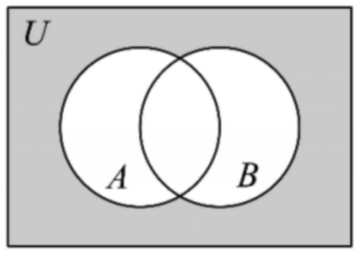
\includegraphics[width=0.20\textwidth]{figures/gao84_q9_venn.png}
\end{center}

\ifanswer
\solbegin
\step{$U=\{1,2,3,4,5,6,7,8,9,10\}$，$A=\{1,2\}$，$B=\{2,4\}$.}
\step{图中阴影部分表示的集合为 $\overline{A\cup B}=\{3,5,6,7,8,9,10\}$，共 $7$ 个元素，}
\step{其非空真子集的个数为 $2^7-2=126$.}
\solend
\fi

\item 若不等式 $ax^2-5x+c<0$ 的解集是 $(2,3)$，则不等式 $cx^2+5x+a\geqslant0$ 的解集是\blankline[4.4em].

\ifanswer
\solbegin
\step{若不等式 $ax^2-5x+c<0$ 的解集是 $(2,3)$，则 $a>0$ 且 $\begin{cases}\dfrac5a=5\\[2pt] \dfrac ca=6\end{cases}$，}
\step{则 $a=1$，$c=6$，}
\step{则不等式 $cx^2+5x+a\geqslant0$ 可化为 $6x^2+5x+1\geqslant0$，则 $x\leqslant-\dfrac12$ 或 $x\geqslant-\dfrac13$，}
\step{则不等式的解集为 $\left(-\infty,-\dfrac12\right]\cup\left[-\dfrac13,+\infty\right)$.}
\solend
\fi

\item 若关于 $x$ 的方程 $mx^2+2x+2=0$ 至少有一个负实根，则实数 $m$ 的取值范围是\blankline[4.4em].

\ifanswer
\solbegin
\step{①当 $m=0$ 时，方程为 $2x+2=0$，有一个负根，满足题意，}
\step{②当 $m\neq0$ 时，关于 $x$ 的方程 $mx^2+2x+2=0$ 至少有一个负根，}
\step{设根为 $x_1$、$x_2$，}
\step{当 $\Delta=4-8m=0$ 时，即 $m=\dfrac12$ 时，方程为 $\dfrac12x^2+2x+1=0$，}
\step{解得 $x=-2$，满足题意，}
\step{当 $\Delta=4-8m>0$，即 $m<\dfrac12$ 时，且 $m\neq0$ 时，}
\step{若有一个负根，则 $x_1x_2=\dfrac2m<0$，解得 $m<0$，}
\step{若有两个负根，则 $\begin{cases}x_1+x_2=-\dfrac2m<0\\[2pt] x_1x_2=\dfrac2m>0\end{cases}$，解得 $0<m<\dfrac12$，}
\step{综上所述，则实数 $m$ 的取值范围是 $\left(-\infty,\dfrac12\right]$.}
\solend
\fi

\item 设集合 $S$、$T$ 都至少含有两个元素，且 $S$、$T$ 同时满足：条件 1：对任意 $x$、$y\in S$，若
$x\neq y$，则 $x+y\in T$；条件 2：对任意 $x$、$y\in T$，若 $x\neq y$，则 $x-y\in S$. 给出下列说法：

①若 $S$ 只有 $2$ 个元素，则这 $2$ 个元素互为相反数；

②若 $S$ 只有 $2$ 个元素，则 $S\cup T$ 必有 $3$ 个元素；

③若 $S$ 只有 $2$ 个元素，则 $S\cup T$ 可能有 $4$ 个元素；

④存在含有 $3$ 个元素的集合 $S$，满足 $S\cup T$ 有 $4$ 个元素.

其中所有正确说法的序号是\blankline[4.4em].

\ifanswer
\solbegin
\step{对于①：由条件 2 得 $x-y\in S$，$y-x\in S$，且 $x-y\neq y-x$，}
\step{所以若 $S$ 只有 $2$ 个元素，则这 $2$ 个元素互为相反数，故①正确；}
\step{对于④：若 $S$ 有 $3$ 个元素，不妨设 $S=\{a,b,c\}$，其中 $a<b<c$，}
\step{则 $\{a+b,b+c,c+a\}\subseteq T$，所以 $c-a$、$c-b$、$b-a$、$a-c$、$b-c$、$a-b\in S$，}
\step{而 $c-a$ 与 $c-b$ 为两个互不相等的正数，$a-c$ 与 $a-b$ 为两个互不相等的负数，}
\step{故集合 $S$ 中至少有 $4$ 个元素，与 $S=\{a,b,c\}$ 有 $3$ 个元素矛盾，故④错误.}
\step{对于②③：若 $S$ 有 $2$ 个元素，由①得集合 $S$ 中的 $2$ 个元素必为相反数，}
\step{故可设 $S=\{a,-a\}(a\neq0)$. 由条件 1 得 $0\in T$，}
\step{由于集合 $T$ 中至少有 $2$ 个元素，故至少还有另外一个元素 $m\in T$.}
\step{当集合 $T$ 只有 $2$ 个元素时即 $T=\{0,m\}$，由条件 1 得 $-m\in S$，则 $m=\pm a$，}
\step{$T=\{0,a\}$ 或 $T=\{0,-a\}$，故 $S\cup T=\{0,a,-a\}$.}
\step{当集合 $T$ 有多于 $2$ 个元素时，不妨设 $T=\{0,m,n\}$，}
\step{则 $m$、$n$、$-m$、$-n$、$m-n$、$n-m\in S$，由于 $m$、$n\neq0$，}
\step{所以 $m\neq m-n$，$n\neq n-m$，又 $m\neq n$，}
\step{故集合 $S$ 至少有 $3$ 个元素，与 $S$ 中只有两个元素矛盾.}
\step{综上，$S\cup T=\{0,a,-a\}$，故②正确，③错误.}
\step{故正确的是①②.}
\solend
\fi

\end{enumerate}

\bigsec{二、选择题}

\begin{enumerate}
\setcounter{enumi}{12}

\item 用反证法证明命题：“若 $x+y>2$，则 $x>1$ 或 $y>1$”时，应假设\mbox{（\quad）}

\keepwithprev
A. $x\leqslant1$ 或 $y\leqslant1$\qquad B. 若 $x>1$ 或 $y>1$

C. $x\leqslant1$ 且 $y\leqslant1$\qquad D. 若 $x>1$ 且 $y>1$

\ifanswer
\ans{$C$}
\fi

\item 下列命题中，为真命题的是\mbox{（\quad）}

\keepwithprev
A. 若 $a>b$，则 $a^2>b^2$\qquad B. 若 $a>b$，$c>d$，则 $ac>bd$

C. 若 $a>b$，则 $\dfrac1a<\dfrac1b$\qquad D. 若 $ac^2>bc^2$，则 $a>b$

\ifanswer
\solbegin
\step{对于 $A$，当 $a=-1$，$b=-2$ 时，$a^2<b^2$，故 $A$ 错误；}
\step{对于 $B$，当 $a=-1$，$b=-2$，$c=-1$，$d=-2$ 时，$ac<bd$，故 $B$ 错误；}
\step{对于 $C$，当 $a=1$，$b=-2$ 时，$\dfrac1a>\dfrac1b$，故 $C$ 错误；}
\step{对于 $D$，因为 $ac^2-bc^2=(a-b)c^2>0$，所以 $a-b>0$，$c^2>0$，则 $a>b$，}
\step{故 $D$ 正确.}
\step{故选 $D$.}
\solend
\fi

\item 现有一级小麦 $m\,\mathrm{kg}$，二级小麦 $n\,\mathrm{kg}$，某粮食收购站有两种收购方案. 方案一：分两个
等级收购小麦，一级小麦 $a$ 元$/\mathrm{kg}$，二级小麦 $b$ 元$/\mathrm{kg}\,(b<a)$；方案二：以方案一两种价
格的平均数收购. 收购方式更加优惠的是\mbox{（\quad）}

\keepwithprev
A. 方案一\qquad B. 方案二\qquad C. 同样优惠\qquad D. 以上均有可能

\ifanswer
\solbegin
\step{方案一收购的平均价格为 $\dfrac{ma+nb}{m+n}$，方案二收购的平均价格为 $\dfrac{a+b}2$；}
\step{所以 $\dfrac{ma+nb}{m+n}-\dfrac{a+b}2=\dfrac{(a-b)(m-n)}{2(m+n)}$ ①，}
\step{$a-b>0$，$m-n$ 的正负性不确定，故①式的正负性不确定，故选 $D$.}
\solend
\fi

\item 用 $C(A)$ 表示非空集合 $A$ 中的元素个数. 对于集合 $A$、$B$，定义

$A*B=\begin{cases}C(A)-C(B),&C(A)\geqslant C(B)\\ C(B)-C(A),&C(A)<C(B)\end{cases}$，若 $A=\{0,1\}$，

$B=\{x\mid(x^2-ax)(x^2+ax+2)=0\}$，设实数 $a$ 的所有可能取值组成的集合是 $S$，则下列选
项不正确的是\mbox{（\quad）}

\keepwithprev
A. $C(B)$ 的可能值为 $1$，$2$，$3$，$4$

B. 若 $A*B=2$，则 $a$ 的取值范围为 $(-\infty,-2\sqrt2)\cup(2\sqrt2,+\infty)$

C. 若 $A*B=1$，则 $C(S)=3$

D. 若 $A*B=0$，则 $a$ 的取值范围为 $(-2\sqrt2,2\sqrt2)$

\ifanswer
\solbegin
\step{对于集合 $B$，当 $a=0$ 时，方程 $x^2(x^2+2)=0$ 的解为 $x=0$，$C(B)=1$，}
\step{当 $a\neq0$ 时，$x^2-ax=0$ 或 $x^2+ax+2=0$，}
\step{其中 $x^2-ax=0$ 的解为 $x_1=0$，$x_2=a$，}
\step{若 $\Delta=a^2-8>0$，即 $a>2\sqrt2$ 或 $a<-2\sqrt2$，}
\step{方程 $x^2+ax+2=0$ 有两个不相等的实数根，此时 $C(B)=4$；}
\step{若 $\Delta=a^2-8=0$，即 $a=2\sqrt2$ 或 $-2\sqrt2$，}
\step{方程 $x^2+ax+2=0$ 有两个相等的实数根，此时 $C(B)=3$；}
\step{若 $\Delta=a^2-8<0$，即 $-2\sqrt2<a<0$ 或 $0<a<2\sqrt2$，}
\step{方程 $x^2+ax+2=0$ 无实数根，此时 $C(B)=2$；}
\step{所以 $C(B)$ 的可能值为 $1$，$2$，$3$，$4$，故 $A$ 正确；}
\step{若 $A*B=2$，且 $C(A)=2$，则 $C(B)=4$，}
\step{则 $a$ 的取值范围 $(-\infty,-2\sqrt2)\cup(2\sqrt2,+\infty)$，故 $B$ 正确；}
\step{若 $A*B=1$，且 $C(A)=2$，则 $C(B)=1$ 或 $3$，}
\step{当 $C(B)=1$ 时，$a=0$，}
\step{当 $C(B)=3$ 时，$a=2\sqrt2$ 或 $-2\sqrt2$，此时集合 $S=\{0,-2\sqrt2,2\sqrt2\}$，}
\step{则 $C(S)=3$，故 $C$ 正确；}
\step{若 $A*B=0$，且 $C(A)=2$，则 $C(B)=2$，}
\step{由此可得 $a$ 的取值范围为 $(-2\sqrt2,0)\cup(0,2\sqrt2)$，故 $D$ 不正确；}
\step{故选 $D$.}
\solend
\fi

\end{enumerate}

\bigsec{三、解答题}

\begin{enumerate}
\setcounter{enumi}{16}

\item 已知集合 $A=\{x\mid-3<x\leqslant4\}$，集合 $B=\{x\mid k+1\leqslant x\leqslant2k-1\}$.

（1）当 $k=3$ 时，求 $A\cup B$、$\overline A\cap B$；

（2）若 $B\subseteq A$，求 $k$ 的取值范围.

\ansspace*[10]

\ifanswer
\solbegin
\stepm{（1）}{当 $k=3$ 时，$B=\{x\mid4\leqslant x\leqslant5\}$，又 $A=\{x\mid-3<x\leqslant4\}$，}
\step{所以 $\overline A=\{x\mid x\leqslant-3$ 或 $x>4\}$，}
\step{所以 $A\cup B=\{x\mid-3<x\leqslant5\}$，$\overline A\cap B=\{x\mid4<x\leqslant5\}$.}
\stepm{（2）}{①当 $B=\varnothing$，即 $k+1>2k-1$ 时，$k<2$，满足 $B\subseteq A$.}
\step{②当 $B\neq\varnothing$ 时，由 $B\subseteq A$ 得 $\begin{cases}k+1\leqslant2k-1\\ k+1>-3\\ 2k-1\leqslant4\end{cases}$，解得 $2\leqslant k\leqslant\dfrac52$，}
\step{综合①②得 $k$ 的取值范围 $\left\{k\mid k\leqslant\dfrac52\right\}$.}
\solend
\fi

\item 设集合 $A=\{x\mid x^2-3x+2=0\}$，$B=\{x\mid x^2+2(a+1)x+a^2-5=0\}$.

（1）若 $A\cap B=\{2\}$，求实数 $a$ 的值；

（2）若集合 $B$ 中有两个元素 $x_1,x_2$，求 $\lvert x_1-x_2\rvert$（用 $a$ 表示）.

\ansspace*[10]

\ifanswer
\solbegin
\stepm{（1）}{由题意得 $A=\{x\mid x^2-3x+2=0\}=\{1,2\}$，因为 $A\cap B=\{2\}$，所以 $2\in B$，}
\step{所以 $2^2+4(a+1)+a^2-5=0$ 即 $4+4a+4+a^2-5=0$，}
\step{化简得 $a^2+4a+3=0$，即 $(a+3)(a+1)=0$，解得 $a=-3$ 或 $a=-1$，}
\step{检验：当 $a=-3$ 时，$B=\{x\mid x^2-4x+4=0\}=\{2\}$，满足 $A\cap B=\{2\}$，}
\step{当 $a=-1$ 时，$B=\{x\mid x^2-4=0\}=\{-2,2\}$，满足 $A\cap B=\{2\}$，}
\step{所以 $a=-3$ 或 $a=-1$.}
\stepm{（2）}{因为 $B$ 中有两个元素 $x_1,x_2$，所以 $x^2+2(a+1)x+(a^2-5)=0$ 有两个根，}
\step{所以 $\Delta=4(a+1)^2-4(a^2-5)=8a+24>0$，}
\step{且 $x_1+x_2=-2(a+1)$，$x_1x_2=a^2-5$，}
\step{所以 $\lvert x_1-x_2\rvert=\sqrt{(x_1+x_2)^2-4x_1x_2}=\sqrt{4(a+1)^2-4(a^2-5)}=\sqrt{8a+24}$.}
\solend
\fi

\item 已知关于 $x$ 的不等式 $\dfrac{ax-2}{1+x}>0$.

（1）若 $x=-a$ 时，不等式成立，求实数 $a$ 的取值范围；

（2）若 $a$ 为实数，解关于 $x$ 的不等式：$\dfrac{ax-2}{1+x}>0$.

\ansspace*[12]

\ifanswer
\solbegin
\stepm{（1）}{因为 $x=-a$ 时，不等式成立，}
\step{所以 $\dfrac{-a^2-2}{1-a}>0\Rightarrow\dfrac{a^2+2}{a-1}>0\Rightarrow a-1>0\Rightarrow a>1$，}
\step{所以实数 $a$ 的取值范围为 $(1,+\infty)$.}
\stepm{（2）}{$\dfrac{ax-2}{1+x}>0\Rightarrow(ax-2)(x+1)>0$，}
\step{当 $a=0$ 时，$-2(x+1)>0$，解得 $x<-1$.}
\step{当 $a>0$ 时，$(ax-2)(x+1)>0$，解得 $x>\dfrac2a$ 或 $x<-1$.}
\step{当 $a<0$ 时，不等式 $(ax-2)(x+1)>0$ 可化为 $\left(x-\dfrac2a\right)(x+1)<0$，}
\step{当 $\dfrac2a>-1$，即 $a<-2$ 时，解得 $-1<x<\dfrac2a$；}
\step{当 $\dfrac2a<-1$，即 $-2<a<0$ 时，解得 $\dfrac2a<x<-1$；}
\step{当 $\dfrac2a=-1$，即 $a=-2$ 时，解集为 $\varnothing$.}
\step{综上，当 $a<-2$ 时，不等式的解集为 $\left(-1,\dfrac2a\right)$；}
\step{当 $a=-2$ 时，不等式的解集为 $\varnothing$；}
\step{当 $-2<a<0$ 时，不等式的解集为 $\left(\dfrac2a,-1\right)$；}
\step{当 $a=0$ 时，不等式的解集为 $(-\infty,-1)$；}
\step{当 $a>0$ 时，不等式的解集为 $(-\infty,-1)\cup\left(\dfrac2a,+\infty\right)$.}
\solend
\fi

\item 已知关于 $x$ 的不等式 $(k^2-2k-3)x^2+(k+1)x+1>0\,(k\in\R)$ 的解集为 $M$；

（1）若存在实数 $a$，使得 $M=(-\infty,a)\cup(a,+\infty)$，求 $k$ 的值；

（2）若 $M=\R$，求 $k$ 的取值范围；

（3）是否存在实数 $k$，满足：“对于任意 $n\in\N$，$n>0$，都有 $n\in M$；对于任意
$m\in\Z$，$m<0$，都有 $m\notin M$”，若存在，求出 $k$ 的值，若不存在，说明理由.

\ansspace*[13]

\ifanswer
\solbegin
\stepm{（1）}{记 $f(x)=(k^2-2k-3)x^2+(k+1)x+1$.}
\step{$M=(-\infty,a)\cup(a,+\infty)$ 表示 $f(x)>0$ 对一切 $x\neq a$ 成立，且 $f(a)=0$，}
\step{故需二次项系数大于 $0$ 且 $\Delta=0$.}
\step{由 $\Delta=(k+1)^2-4(k^2-2k-3)=-3k^2+10k+13=0$ 得 $k=\dfrac{13}3$ 或 $k=-1$.}
\step{当 $k=\dfrac{13}3$ 时，二次项系数 $\dfrac{64}9>0$，$f(x)=\dfrac{64}9\left(x+\dfrac38\right)^2$，符合；}
\step{当 $k=-1$ 时二次项系数为 $0$，$f(x)=1>0$，$M=\R$，不符合. 故 $k=\dfrac{13}3$.}
\stepm{（2）}{$M=\R$ 即 $f(x)>0$ 对一切 $x\in\R$ 恒成立.}
\step{①当 $k^2-2k-3>0$（即 $k<-1$ 或 $k>3$）时，需 $\Delta<0$，}
\step{即 $-3k^2+10k+13<0$，得 $k<-1$ 或 $k>\dfrac{13}3$，故 $k<-1$ 或 $k>\dfrac{13}3$；}
\step{②当 $k^2-2k-3=0$ 时，$k=3$ 得 $f(x)=4x+1$ 不恒正，不符合题意，}
\step{舍去，}
\step{当 $k=-1$ 得 $f(x)=1>0$ 恒成立，符合题意；}
\step{③当 $k^2-2k-3<0$ 时，抛物线开口向下，不能恒正.}
\step{综上，$k\leqslant-1$ 或 $k>\dfrac{13}3$.}
\stepm{（3）}{存在，$k=3$，理由如下，}
\step{由题意得解集 $M=(t,+\infty)$，$t\in[-1,1)$；}
\step{当 $k^2-2k-3=0$ 时，解得 $k=3$ 或 $k=-1$，}
\step{$k=3$ 时，不等式的解集为 $\left(-\dfrac14,+\infty\right)$，满足条件；}
\step{$k=-1$ 时，$1>0$ 恒成立，不满足条件；}
\step{当 $k^2-2k-3>0$ 时，}
\step{此时对应的一元二次不等式的解集形式不是 $(t,+\infty)$ 的形式，不满足条件；}
\step{当 $k^2-2k-3<0$ 时，}
\step{此时对应的一元二次不等式的解集形式不是 $(t,+\infty)$ 的形式，不满足条件；}
\step{综上，满足条件 $k$ 的值为 $3$.}
\solend
\fi

\item 已知有限集 $A=\{a_1,a_2,\cdots,a_n\}\,(n\geqslant2,n\in\N)$，如果 $A$ 中元素 $a_i\,(i=1,2,3,\cdots,n)$ 满足
$a_1+a_2+a_3+\cdots+a_n=a_1\times a_2\times\cdots\times a_n$，就称 $A$ 为“和积平衡集”.

（1）判断集合 $\{-1+\sqrt3,-1-\sqrt3\}$ 是否为“和积平衡集”；

（2）若 $a_1$、$a_2$ 是两个不同的正数，且 $\{a_1,a_2\}$ 是“和积平衡集”，写出以 $a_1$、$a_2$ 为根的一
个一元二次方程（系数可用 $a_1$、$a_2$ 表示），并证明 $a_1$、$a_2$ 至少有一个大于 $2$；

（3）若 $a_i\in\Z$ 且 $a_i>0$，求所有符合条件的“和积平衡集”.

\ansspace*[14]

\ifanswer
\solbegin
\stepm{（1）}{对于集合 $\{-1+\sqrt3,-1-\sqrt3\}$，}
\step{因为 $(-1+\sqrt3)+(-1-\sqrt3)=-2$，$(-1+\sqrt3)\times(-1-\sqrt3)=-2$，}
\step{所以满足 $a_1+a_2=a_1\times a_2$，满足题意，}
\step{所以集合 $\{-1+\sqrt3,-1-\sqrt3\}$ 是和积平衡集.}
\stepm{（2）}{以 $a_1$、$a_2$ 为根的一个一元二次方程可为 $x^2-(a_1+a_2)x+a_1\cdot a_2=0$，}
\step{因为 $a_1$、$a_2$ 是两个不同的正数，且 $\{a_1,a_2\}$ 是和积平衡集，}
\step{所以 $a_1+a_2=a_1\cdot a_2$，}
\step{又 $a_1$ 和 $a_2$ 为 $x^2-(a_1+a_2)x+a_1\cdot a_2=0$ 的两个不同的正根，}
\step{所以 $\Delta=(a_1+a_2)^2-4a_1a_2=(a_1+a_2)^2-4(a_1+a_2)>0$，}
\step{又 $a_1+a_2>0$，则 $a_1+a_2>4$，}
\step{若 $a_1$、$a_2$ 都小于等于 $2$，则 $a_1+a_2\leqslant4$，矛盾，}
\step{所以 $a_1$、$a_2$ 至少有一个大于 $2$；}
\stepm{（3）}{设 $A$ 中的 $a_1<a_2<a_3<\cdots<a_n$，且 $a_i\in\N^*$，}
\step{由 $a_1+a_2+a_3+\cdots+a_n=a_1\times a_2\times\cdots\times a_n$，得 $n=2$ 时明显不满足，}
\step{所以 $n\geqslant3$，故 $a_1\times a_2\times\cdots\times a_n=a_1+a_2+a_3+\cdots+a_n\leqslant na_n$，}
\step{所以 $a_1\times a_2\times\cdots\times a_{n-1}\leqslant n$，}
\step{当 $n=3$ 时，$a_1\times a_2\leqslant3$，$a_i\in\N^*$，只能有 $a_1=1$，$a_2=2$，}
\step{由 $a_1+a_2+a_3=a_1\times a_2\times a_3$，得 $a_3=3$，此时的和积平衡集为 $\{1,2,3\}$，}
\step{当 $n\geqslant4$ 时，$a_1\times a_2\times\cdots\times a_{n-1}\geqslant(n-1)(n-2)\times\cdots\times2\times1\geqslant(n-1)(n-2)$，}
\step{又 $(n-1)(n-2)-n=n^2-4n+2=n(n-4)+2>0$，即 $(n-1)(n-2)>n$，}
\step{即 $a_1\times a_2\times\cdots\times a_{n-1}>n$，与 $a_1\times a_2\times\cdots\times a_{n-1}\leqslant n$ 矛盾，}
\step{所以 $n\geqslant4$ 不满足条件，}
\step{所以符合条件的和积平衡集有且只有 $n=3$，此时的和积平衡集为 $\{1,2,3\}$.}
\solend
\fi

\end{enumerate}

\end{document}
"
% 紧凑版：xelatex "\def\iscompact{1}% 高一84_东昌中学_10月月考.tex
%   —— 高一上数学“2026-2027 年东昌中学高一上 10 月月考”（讲评版）
% 试卷版：xelatex 高一84_东昌中学_10月月考.tex
% 答案版：xelatex "\def\isanswer{1}\input{高一84_东昌中学_10月月考.tex}"
% 紧凑版：xelatex "\def\iscompact{1}\input{高一84_东昌中学_10月月考.tex}"
%
% 原始材料：微信公众号“魔都数学加油站”文章，连载“27学年高一84”；
% 原文标题“27学年高一84——2026-2027年上海市东昌中学高一上10月月考”；
% 原文链接：https://mp.weixin.qq.com/s/PErsjO3N5RsMuJC69IGbrw。
% 页面标注发布时间 2026-10-26 20:15（上海）。
% 正文为 12 张 PNG 页（`原图/高一84_东昌中学_10月月考/01..12.png`），
% 尺寸混排（第 1—8 页为 4762×6735，第 9—12 页为 2560×3620），均按页序读取。
%
% 篇幅与题号：原卷自第 3 题起编号（第 1、2 题不在原文内）。填空题 3—12（10 题）、
% 选择题 13—16（4 题）、解答题 17—21（5 题），共 19 题。
%
% 讲评版：19 题全部印【解析】，本稿不另提 \ans{}；选择题答案在解析末句“故选 D／C／D”。
% 第 13 题的答案“C”原卷直接印在题干括号内（“（\ C\ ）”），本稿按 高一37 第 13 题／
% 高一63 第 14 题成例括号留空、另提 \ans{$C$}（该题无【解析】段）。
%
% 副标题：原卷未印副标题。本稿按内容标作“集合与常用逻辑用语、不等式”。
%
% 与原卷的排版差异：
%   ① 原卷每题下直接印【解析】，本稿按全稿惯例将解析置于答案版；
%   ② 原卷未印副标题，本稿补出；填空横线统一排 \blankline[4.4em]；
%   ③ 原卷数集记号排斜体 $R$、$Z$、$N$，本稿按全稿惯例改用 $\R$、$\Z$、$\N$；
%   ④ 第 17—21 题的子问用行内“（1）（2）（3）”段，解析中的子问标号用 \stepm；
%   ⑤ 解答题按惯例加 \ansspace；选择题括号排 \mbox{（\quad）}；
%   ⑥ 第 9 题题干右侧有一幅韦恩图，裁自原图（第 2 页）后去粉色水印、转灰度，
%      三版都出（属题干）。
%
% 行数核对：逐题数 \step/\stepm 条数，合计 157 条（Q3：2；Q4：2；Q5：3；Q6：2；
% Q7：3；Q8：6；Q9：3；Q10：4；Q11：9；Q12：17；Q14：6；Q15：3；Q16：19；
% Q17：6；Q18：10；Q19：15；Q20：24；Q21：23）；第 13 题无解析，只提 \ans{}，
% 不计入 \step 账。原卷解析的换行按语意合并，未逐行强拆。
%
\documentclass[a4paper,11pt]{article}
\usepackage{common}

\begin{document}

\examtitlest[4]{2026--2027 年东昌中学高一上 10 月月考}{集合与常用逻辑用语、不等式}

\bigsec{一、填空题}

\begin{enumerate}
\setcounter{enumi}{2}

\item 若 $a\in\R$，则“$a=2$”是“$(a-1)(a-2)=0$”的\blankline[3.6em]条件（填“充分不必要”、“必要
不充分”、“充要”、“既不充分又不必要”的一个）.

\ifanswer
\solbegin
\step{$a=2\Rightarrow(a-1)(a-2)=0$，而 $(a-1)(a-2)=0$ 不能推出 $a=2$，}
\step{故“$a=2$”是“$(a-1)(a-2)=0$”的充分不必要条件.}
\solend
\fi

\item 已知集合 $M=\{(x,y)\mid y=x^2\}$，$N=\{(x,y)\mid y=1\}$，则 $M\cap N=\blankline[4.4em]$.

\ifanswer
\solbegin
\step{集合 $M=\{(x,y)\mid y=x^2\}$，$N=\{(x,y)\mid y=1\}$，}
\step{当 $y=1$ 时，$x=\pm1$，则 $M\cap N=\{(-1,1),(1,1)\}$.}
\solend
\fi

\item 已知集合 $A=\{x\mid x^2+ax+4=0\}$，若 $A$ 有且只有一个非空子集，则实数 $a=\blankline[4.4em]$.

\ifanswer
\solbegin
\step{因为集合 $A$ 有且只有一个非空子集，所以集合 $A$ 中只有一个元素，}
\step{所以一元二次方程 $x^2+ax+4=0$ 有两个相等的解，}
\step{所以 $\Delta=a^2-4\times4=0$，解得 $a=\pm4$.}
\solend
\fi

\item 已知 $A=(-\infty,a]$，$B=(-\infty,3)$，且 $x\in A$ 是 $x\in B$ 的充分不必要条件，则 $a$ 的取值范围
是\blankline[4.4em].

\ifanswer
\solbegin
\step{$A=(-\infty,a]$，$B=(-\infty,3)$，且 $x\in A$ 是 $x\in B$ 的充分不必要条件，}
\step{则 $A\subset B$，则 $a<3$，即 $a$ 的取值范围为 $(-\infty,3)$.}
\solend
\fi

\item 不等式 $\dfrac{3x-1}{x-2}\leqslant1$ 的解集为\blankline[4.4em].

\ifanswer
\solbegin
\step{由 $\dfrac{3x-1}{x-2}\leqslant1$，得 $\dfrac{3x-1}{x-2}-1=\dfrac{3x-1-(x-2)}{x-2}=\dfrac{2x+1}{x-2}\leqslant0$，}
\step{则 $\begin{cases}(2x+1)(x-2)\leqslant0\\ x-2\neq0\end{cases}$，解得 $-\dfrac12\leqslant x<2$，}
\step{则不等式 $\dfrac{3x-1}{x-2}\leqslant1$ 的解集为 $\left[-\dfrac12,2\right)$.}
\solend
\fi

\item 已知关于 $x$ 的一元二次方程 $x^2-2mx+(3m+1)=0$ 的两个实数根为 $x_1$、$x_2$，且
$x_1^2+x_2^2=16$，则实数 $m$ 的值为\blankline[4.4em].

\ifanswer
\solbegin
\step{由韦达定理，得 $x_1+x_2=2m$，$x_1x_2=3m+1$，}
\step{$x_1^2+x_2^2=(x_1+x_2)^2-2x_1x_2=4m^2-6m-2$，}
\step{由 $x_1^2+x_2^2=16$，得 $4m^2-6m-2=16$，即 $2m^2-3m-9=0$，}
\step{解得 $m=3$ 或 $m=-\dfrac32$，}
\step{检验判别式 $\Delta=4m^2-12m-4$，当 $m=3$ 时，$\Delta=-4<0$，舍去；}
\step{当 $m=-\dfrac32$ 时，$\Delta=23>0$，符合条件，故 $m=-\dfrac32$.}
\solend
\fi

\item 已知全集 $U=\{x\mid1\leqslant x\leqslant10,\,x\in\N\}$，集合 $A=\{x\mid x^2-3<4,\,x\in\N,\,x>0\}$，
$B=\{2,4\}$，则图中阴影部分表示的集合的非空真子集个数为\blankline[4.4em].

\needvspace{9\baselineskip}
\begin{center}
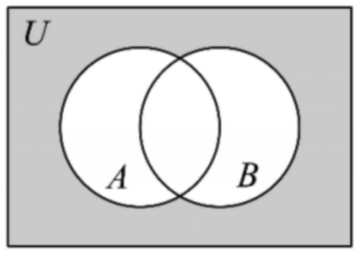
\includegraphics[width=0.20\textwidth]{figures/gao84_q9_venn.png}
\end{center}

\ifanswer
\solbegin
\step{$U=\{1,2,3,4,5,6,7,8,9,10\}$，$A=\{1,2\}$，$B=\{2,4\}$.}
\step{图中阴影部分表示的集合为 $\overline{A\cup B}=\{3,5,6,7,8,9,10\}$，共 $7$ 个元素，}
\step{其非空真子集的个数为 $2^7-2=126$.}
\solend
\fi

\item 若不等式 $ax^2-5x+c<0$ 的解集是 $(2,3)$，则不等式 $cx^2+5x+a\geqslant0$ 的解集是\blankline[4.4em].

\ifanswer
\solbegin
\step{若不等式 $ax^2-5x+c<0$ 的解集是 $(2,3)$，则 $a>0$ 且 $\begin{cases}\dfrac5a=5\\[2pt] \dfrac ca=6\end{cases}$，}
\step{则 $a=1$，$c=6$，}
\step{则不等式 $cx^2+5x+a\geqslant0$ 可化为 $6x^2+5x+1\geqslant0$，则 $x\leqslant-\dfrac12$ 或 $x\geqslant-\dfrac13$，}
\step{则不等式的解集为 $\left(-\infty,-\dfrac12\right]\cup\left[-\dfrac13,+\infty\right)$.}
\solend
\fi

\item 若关于 $x$ 的方程 $mx^2+2x+2=0$ 至少有一个负实根，则实数 $m$ 的取值范围是\blankline[4.4em].

\ifanswer
\solbegin
\step{①当 $m=0$ 时，方程为 $2x+2=0$，有一个负根，满足题意，}
\step{②当 $m\neq0$ 时，关于 $x$ 的方程 $mx^2+2x+2=0$ 至少有一个负根，}
\step{设根为 $x_1$、$x_2$，}
\step{当 $\Delta=4-8m=0$ 时，即 $m=\dfrac12$ 时，方程为 $\dfrac12x^2+2x+1=0$，}
\step{解得 $x=-2$，满足题意，}
\step{当 $\Delta=4-8m>0$，即 $m<\dfrac12$ 时，且 $m\neq0$ 时，}
\step{若有一个负根，则 $x_1x_2=\dfrac2m<0$，解得 $m<0$，}
\step{若有两个负根，则 $\begin{cases}x_1+x_2=-\dfrac2m<0\\[2pt] x_1x_2=\dfrac2m>0\end{cases}$，解得 $0<m<\dfrac12$，}
\step{综上所述，则实数 $m$ 的取值范围是 $\left(-\infty,\dfrac12\right]$.}
\solend
\fi

\item 设集合 $S$、$T$ 都至少含有两个元素，且 $S$、$T$ 同时满足：条件 1：对任意 $x$、$y\in S$，若
$x\neq y$，则 $x+y\in T$；条件 2：对任意 $x$、$y\in T$，若 $x\neq y$，则 $x-y\in S$. 给出下列说法：

①若 $S$ 只有 $2$ 个元素，则这 $2$ 个元素互为相反数；

②若 $S$ 只有 $2$ 个元素，则 $S\cup T$ 必有 $3$ 个元素；

③若 $S$ 只有 $2$ 个元素，则 $S\cup T$ 可能有 $4$ 个元素；

④存在含有 $3$ 个元素的集合 $S$，满足 $S\cup T$ 有 $4$ 个元素.

其中所有正确说法的序号是\blankline[4.4em].

\ifanswer
\solbegin
\step{对于①：由条件 2 得 $x-y\in S$，$y-x\in S$，且 $x-y\neq y-x$，}
\step{所以若 $S$ 只有 $2$ 个元素，则这 $2$ 个元素互为相反数，故①正确；}
\step{对于④：若 $S$ 有 $3$ 个元素，不妨设 $S=\{a,b,c\}$，其中 $a<b<c$，}
\step{则 $\{a+b,b+c,c+a\}\subseteq T$，所以 $c-a$、$c-b$、$b-a$、$a-c$、$b-c$、$a-b\in S$，}
\step{而 $c-a$ 与 $c-b$ 为两个互不相等的正数，$a-c$ 与 $a-b$ 为两个互不相等的负数，}
\step{故集合 $S$ 中至少有 $4$ 个元素，与 $S=\{a,b,c\}$ 有 $3$ 个元素矛盾，故④错误.}
\step{对于②③：若 $S$ 有 $2$ 个元素，由①得集合 $S$ 中的 $2$ 个元素必为相反数，}
\step{故可设 $S=\{a,-a\}(a\neq0)$. 由条件 1 得 $0\in T$，}
\step{由于集合 $T$ 中至少有 $2$ 个元素，故至少还有另外一个元素 $m\in T$.}
\step{当集合 $T$ 只有 $2$ 个元素时即 $T=\{0,m\}$，由条件 1 得 $-m\in S$，则 $m=\pm a$，}
\step{$T=\{0,a\}$ 或 $T=\{0,-a\}$，故 $S\cup T=\{0,a,-a\}$.}
\step{当集合 $T$ 有多于 $2$ 个元素时，不妨设 $T=\{0,m,n\}$，}
\step{则 $m$、$n$、$-m$、$-n$、$m-n$、$n-m\in S$，由于 $m$、$n\neq0$，}
\step{所以 $m\neq m-n$，$n\neq n-m$，又 $m\neq n$，}
\step{故集合 $S$ 至少有 $3$ 个元素，与 $S$ 中只有两个元素矛盾.}
\step{综上，$S\cup T=\{0,a,-a\}$，故②正确，③错误.}
\step{故正确的是①②.}
\solend
\fi

\end{enumerate}

\bigsec{二、选择题}

\begin{enumerate}
\setcounter{enumi}{12}

\item 用反证法证明命题：“若 $x+y>2$，则 $x>1$ 或 $y>1$”时，应假设\mbox{（\quad）}

\keepwithprev
A. $x\leqslant1$ 或 $y\leqslant1$\qquad B. 若 $x>1$ 或 $y>1$

C. $x\leqslant1$ 且 $y\leqslant1$\qquad D. 若 $x>1$ 且 $y>1$

\ifanswer
\ans{$C$}
\fi

\item 下列命题中，为真命题的是\mbox{（\quad）}

\keepwithprev
A. 若 $a>b$，则 $a^2>b^2$\qquad B. 若 $a>b$，$c>d$，则 $ac>bd$

C. 若 $a>b$，则 $\dfrac1a<\dfrac1b$\qquad D. 若 $ac^2>bc^2$，则 $a>b$

\ifanswer
\solbegin
\step{对于 $A$，当 $a=-1$，$b=-2$ 时，$a^2<b^2$，故 $A$ 错误；}
\step{对于 $B$，当 $a=-1$，$b=-2$，$c=-1$，$d=-2$ 时，$ac<bd$，故 $B$ 错误；}
\step{对于 $C$，当 $a=1$，$b=-2$ 时，$\dfrac1a>\dfrac1b$，故 $C$ 错误；}
\step{对于 $D$，因为 $ac^2-bc^2=(a-b)c^2>0$，所以 $a-b>0$，$c^2>0$，则 $a>b$，}
\step{故 $D$ 正确.}
\step{故选 $D$.}
\solend
\fi

\item 现有一级小麦 $m\,\mathrm{kg}$，二级小麦 $n\,\mathrm{kg}$，某粮食收购站有两种收购方案. 方案一：分两个
等级收购小麦，一级小麦 $a$ 元$/\mathrm{kg}$，二级小麦 $b$ 元$/\mathrm{kg}\,(b<a)$；方案二：以方案一两种价
格的平均数收购. 收购方式更加优惠的是\mbox{（\quad）}

\keepwithprev
A. 方案一\qquad B. 方案二\qquad C. 同样优惠\qquad D. 以上均有可能

\ifanswer
\solbegin
\step{方案一收购的平均价格为 $\dfrac{ma+nb}{m+n}$，方案二收购的平均价格为 $\dfrac{a+b}2$；}
\step{所以 $\dfrac{ma+nb}{m+n}-\dfrac{a+b}2=\dfrac{(a-b)(m-n)}{2(m+n)}$ ①，}
\step{$a-b>0$，$m-n$ 的正负性不确定，故①式的正负性不确定，故选 $D$.}
\solend
\fi

\item 用 $C(A)$ 表示非空集合 $A$ 中的元素个数. 对于集合 $A$、$B$，定义

$A*B=\begin{cases}C(A)-C(B),&C(A)\geqslant C(B)\\ C(B)-C(A),&C(A)<C(B)\end{cases}$，若 $A=\{0,1\}$，

$B=\{x\mid(x^2-ax)(x^2+ax+2)=0\}$，设实数 $a$ 的所有可能取值组成的集合是 $S$，则下列选
项不正确的是\mbox{（\quad）}

\keepwithprev
A. $C(B)$ 的可能值为 $1$，$2$，$3$，$4$

B. 若 $A*B=2$，则 $a$ 的取值范围为 $(-\infty,-2\sqrt2)\cup(2\sqrt2,+\infty)$

C. 若 $A*B=1$，则 $C(S)=3$

D. 若 $A*B=0$，则 $a$ 的取值范围为 $(-2\sqrt2,2\sqrt2)$

\ifanswer
\solbegin
\step{对于集合 $B$，当 $a=0$ 时，方程 $x^2(x^2+2)=0$ 的解为 $x=0$，$C(B)=1$，}
\step{当 $a\neq0$ 时，$x^2-ax=0$ 或 $x^2+ax+2=0$，}
\step{其中 $x^2-ax=0$ 的解为 $x_1=0$，$x_2=a$，}
\step{若 $\Delta=a^2-8>0$，即 $a>2\sqrt2$ 或 $a<-2\sqrt2$，}
\step{方程 $x^2+ax+2=0$ 有两个不相等的实数根，此时 $C(B)=4$；}
\step{若 $\Delta=a^2-8=0$，即 $a=2\sqrt2$ 或 $-2\sqrt2$，}
\step{方程 $x^2+ax+2=0$ 有两个相等的实数根，此时 $C(B)=3$；}
\step{若 $\Delta=a^2-8<0$，即 $-2\sqrt2<a<0$ 或 $0<a<2\sqrt2$，}
\step{方程 $x^2+ax+2=0$ 无实数根，此时 $C(B)=2$；}
\step{所以 $C(B)$ 的可能值为 $1$，$2$，$3$，$4$，故 $A$ 正确；}
\step{若 $A*B=2$，且 $C(A)=2$，则 $C(B)=4$，}
\step{则 $a$ 的取值范围 $(-\infty,-2\sqrt2)\cup(2\sqrt2,+\infty)$，故 $B$ 正确；}
\step{若 $A*B=1$，且 $C(A)=2$，则 $C(B)=1$ 或 $3$，}
\step{当 $C(B)=1$ 时，$a=0$，}
\step{当 $C(B)=3$ 时，$a=2\sqrt2$ 或 $-2\sqrt2$，此时集合 $S=\{0,-2\sqrt2,2\sqrt2\}$，}
\step{则 $C(S)=3$，故 $C$ 正确；}
\step{若 $A*B=0$，且 $C(A)=2$，则 $C(B)=2$，}
\step{由此可得 $a$ 的取值范围为 $(-2\sqrt2,0)\cup(0,2\sqrt2)$，故 $D$ 不正确；}
\step{故选 $D$.}
\solend
\fi

\end{enumerate}

\bigsec{三、解答题}

\begin{enumerate}
\setcounter{enumi}{16}

\item 已知集合 $A=\{x\mid-3<x\leqslant4\}$，集合 $B=\{x\mid k+1\leqslant x\leqslant2k-1\}$.

（1）当 $k=3$ 时，求 $A\cup B$、$\overline A\cap B$；

（2）若 $B\subseteq A$，求 $k$ 的取值范围.

\ansspace*[10]

\ifanswer
\solbegin
\stepm{（1）}{当 $k=3$ 时，$B=\{x\mid4\leqslant x\leqslant5\}$，又 $A=\{x\mid-3<x\leqslant4\}$，}
\step{所以 $\overline A=\{x\mid x\leqslant-3$ 或 $x>4\}$，}
\step{所以 $A\cup B=\{x\mid-3<x\leqslant5\}$，$\overline A\cap B=\{x\mid4<x\leqslant5\}$.}
\stepm{（2）}{①当 $B=\varnothing$，即 $k+1>2k-1$ 时，$k<2$，满足 $B\subseteq A$.}
\step{②当 $B\neq\varnothing$ 时，由 $B\subseteq A$ 得 $\begin{cases}k+1\leqslant2k-1\\ k+1>-3\\ 2k-1\leqslant4\end{cases}$，解得 $2\leqslant k\leqslant\dfrac52$，}
\step{综合①②得 $k$ 的取值范围 $\left\{k\mid k\leqslant\dfrac52\right\}$.}
\solend
\fi

\item 设集合 $A=\{x\mid x^2-3x+2=0\}$，$B=\{x\mid x^2+2(a+1)x+a^2-5=0\}$.

（1）若 $A\cap B=\{2\}$，求实数 $a$ 的值；

（2）若集合 $B$ 中有两个元素 $x_1,x_2$，求 $\lvert x_1-x_2\rvert$（用 $a$ 表示）.

\ansspace*[10]

\ifanswer
\solbegin
\stepm{（1）}{由题意得 $A=\{x\mid x^2-3x+2=0\}=\{1,2\}$，因为 $A\cap B=\{2\}$，所以 $2\in B$，}
\step{所以 $2^2+4(a+1)+a^2-5=0$ 即 $4+4a+4+a^2-5=0$，}
\step{化简得 $a^2+4a+3=0$，即 $(a+3)(a+1)=0$，解得 $a=-3$ 或 $a=-1$，}
\step{检验：当 $a=-3$ 时，$B=\{x\mid x^2-4x+4=0\}=\{2\}$，满足 $A\cap B=\{2\}$，}
\step{当 $a=-1$ 时，$B=\{x\mid x^2-4=0\}=\{-2,2\}$，满足 $A\cap B=\{2\}$，}
\step{所以 $a=-3$ 或 $a=-1$.}
\stepm{（2）}{因为 $B$ 中有两个元素 $x_1,x_2$，所以 $x^2+2(a+1)x+(a^2-5)=0$ 有两个根，}
\step{所以 $\Delta=4(a+1)^2-4(a^2-5)=8a+24>0$，}
\step{且 $x_1+x_2=-2(a+1)$，$x_1x_2=a^2-5$，}
\step{所以 $\lvert x_1-x_2\rvert=\sqrt{(x_1+x_2)^2-4x_1x_2}=\sqrt{4(a+1)^2-4(a^2-5)}=\sqrt{8a+24}$.}
\solend
\fi

\item 已知关于 $x$ 的不等式 $\dfrac{ax-2}{1+x}>0$.

（1）若 $x=-a$ 时，不等式成立，求实数 $a$ 的取值范围；

（2）若 $a$ 为实数，解关于 $x$ 的不等式：$\dfrac{ax-2}{1+x}>0$.

\ansspace*[12]

\ifanswer
\solbegin
\stepm{（1）}{因为 $x=-a$ 时，不等式成立，}
\step{所以 $\dfrac{-a^2-2}{1-a}>0\Rightarrow\dfrac{a^2+2}{a-1}>0\Rightarrow a-1>0\Rightarrow a>1$，}
\step{所以实数 $a$ 的取值范围为 $(1,+\infty)$.}
\stepm{（2）}{$\dfrac{ax-2}{1+x}>0\Rightarrow(ax-2)(x+1)>0$，}
\step{当 $a=0$ 时，$-2(x+1)>0$，解得 $x<-1$.}
\step{当 $a>0$ 时，$(ax-2)(x+1)>0$，解得 $x>\dfrac2a$ 或 $x<-1$.}
\step{当 $a<0$ 时，不等式 $(ax-2)(x+1)>0$ 可化为 $\left(x-\dfrac2a\right)(x+1)<0$，}
\step{当 $\dfrac2a>-1$，即 $a<-2$ 时，解得 $-1<x<\dfrac2a$；}
\step{当 $\dfrac2a<-1$，即 $-2<a<0$ 时，解得 $\dfrac2a<x<-1$；}
\step{当 $\dfrac2a=-1$，即 $a=-2$ 时，解集为 $\varnothing$.}
\step{综上，当 $a<-2$ 时，不等式的解集为 $\left(-1,\dfrac2a\right)$；}
\step{当 $a=-2$ 时，不等式的解集为 $\varnothing$；}
\step{当 $-2<a<0$ 时，不等式的解集为 $\left(\dfrac2a,-1\right)$；}
\step{当 $a=0$ 时，不等式的解集为 $(-\infty,-1)$；}
\step{当 $a>0$ 时，不等式的解集为 $(-\infty,-1)\cup\left(\dfrac2a,+\infty\right)$.}
\solend
\fi

\item 已知关于 $x$ 的不等式 $(k^2-2k-3)x^2+(k+1)x+1>0\,(k\in\R)$ 的解集为 $M$；

（1）若存在实数 $a$，使得 $M=(-\infty,a)\cup(a,+\infty)$，求 $k$ 的值；

（2）若 $M=\R$，求 $k$ 的取值范围；

（3）是否存在实数 $k$，满足：“对于任意 $n\in\N$，$n>0$，都有 $n\in M$；对于任意
$m\in\Z$，$m<0$，都有 $m\notin M$”，若存在，求出 $k$ 的值，若不存在，说明理由.

\ansspace*[13]

\ifanswer
\solbegin
\stepm{（1）}{记 $f(x)=(k^2-2k-3)x^2+(k+1)x+1$.}
\step{$M=(-\infty,a)\cup(a,+\infty)$ 表示 $f(x)>0$ 对一切 $x\neq a$ 成立，且 $f(a)=0$，}
\step{故需二次项系数大于 $0$ 且 $\Delta=0$.}
\step{由 $\Delta=(k+1)^2-4(k^2-2k-3)=-3k^2+10k+13=0$ 得 $k=\dfrac{13}3$ 或 $k=-1$.}
\step{当 $k=\dfrac{13}3$ 时，二次项系数 $\dfrac{64}9>0$，$f(x)=\dfrac{64}9\left(x+\dfrac38\right)^2$，符合；}
\step{当 $k=-1$ 时二次项系数为 $0$，$f(x)=1>0$，$M=\R$，不符合. 故 $k=\dfrac{13}3$.}
\stepm{（2）}{$M=\R$ 即 $f(x)>0$ 对一切 $x\in\R$ 恒成立.}
\step{①当 $k^2-2k-3>0$（即 $k<-1$ 或 $k>3$）时，需 $\Delta<0$，}
\step{即 $-3k^2+10k+13<0$，得 $k<-1$ 或 $k>\dfrac{13}3$，故 $k<-1$ 或 $k>\dfrac{13}3$；}
\step{②当 $k^2-2k-3=0$ 时，$k=3$ 得 $f(x)=4x+1$ 不恒正，不符合题意，}
\step{舍去，}
\step{当 $k=-1$ 得 $f(x)=1>0$ 恒成立，符合题意；}
\step{③当 $k^2-2k-3<0$ 时，抛物线开口向下，不能恒正.}
\step{综上，$k\leqslant-1$ 或 $k>\dfrac{13}3$.}
\stepm{（3）}{存在，$k=3$，理由如下，}
\step{由题意得解集 $M=(t,+\infty)$，$t\in[-1,1)$；}
\step{当 $k^2-2k-3=0$ 时，解得 $k=3$ 或 $k=-1$，}
\step{$k=3$ 时，不等式的解集为 $\left(-\dfrac14,+\infty\right)$，满足条件；}
\step{$k=-1$ 时，$1>0$ 恒成立，不满足条件；}
\step{当 $k^2-2k-3>0$ 时，}
\step{此时对应的一元二次不等式的解集形式不是 $(t,+\infty)$ 的形式，不满足条件；}
\step{当 $k^2-2k-3<0$ 时，}
\step{此时对应的一元二次不等式的解集形式不是 $(t,+\infty)$ 的形式，不满足条件；}
\step{综上，满足条件 $k$ 的值为 $3$.}
\solend
\fi

\item 已知有限集 $A=\{a_1,a_2,\cdots,a_n\}\,(n\geqslant2,n\in\N)$，如果 $A$ 中元素 $a_i\,(i=1,2,3,\cdots,n)$ 满足
$a_1+a_2+a_3+\cdots+a_n=a_1\times a_2\times\cdots\times a_n$，就称 $A$ 为“和积平衡集”.

（1）判断集合 $\{-1+\sqrt3,-1-\sqrt3\}$ 是否为“和积平衡集”；

（2）若 $a_1$、$a_2$ 是两个不同的正数，且 $\{a_1,a_2\}$ 是“和积平衡集”，写出以 $a_1$、$a_2$ 为根的一
个一元二次方程（系数可用 $a_1$、$a_2$ 表示），并证明 $a_1$、$a_2$ 至少有一个大于 $2$；

（3）若 $a_i\in\Z$ 且 $a_i>0$，求所有符合条件的“和积平衡集”.

\ansspace*[14]

\ifanswer
\solbegin
\stepm{（1）}{对于集合 $\{-1+\sqrt3,-1-\sqrt3\}$，}
\step{因为 $(-1+\sqrt3)+(-1-\sqrt3)=-2$，$(-1+\sqrt3)\times(-1-\sqrt3)=-2$，}
\step{所以满足 $a_1+a_2=a_1\times a_2$，满足题意，}
\step{所以集合 $\{-1+\sqrt3,-1-\sqrt3\}$ 是和积平衡集.}
\stepm{（2）}{以 $a_1$、$a_2$ 为根的一个一元二次方程可为 $x^2-(a_1+a_2)x+a_1\cdot a_2=0$，}
\step{因为 $a_1$、$a_2$ 是两个不同的正数，且 $\{a_1,a_2\}$ 是和积平衡集，}
\step{所以 $a_1+a_2=a_1\cdot a_2$，}
\step{又 $a_1$ 和 $a_2$ 为 $x^2-(a_1+a_2)x+a_1\cdot a_2=0$ 的两个不同的正根，}
\step{所以 $\Delta=(a_1+a_2)^2-4a_1a_2=(a_1+a_2)^2-4(a_1+a_2)>0$，}
\step{又 $a_1+a_2>0$，则 $a_1+a_2>4$，}
\step{若 $a_1$、$a_2$ 都小于等于 $2$，则 $a_1+a_2\leqslant4$，矛盾，}
\step{所以 $a_1$、$a_2$ 至少有一个大于 $2$；}
\stepm{（3）}{设 $A$ 中的 $a_1<a_2<a_3<\cdots<a_n$，且 $a_i\in\N^*$，}
\step{由 $a_1+a_2+a_3+\cdots+a_n=a_1\times a_2\times\cdots\times a_n$，得 $n=2$ 时明显不满足，}
\step{所以 $n\geqslant3$，故 $a_1\times a_2\times\cdots\times a_n=a_1+a_2+a_3+\cdots+a_n\leqslant na_n$，}
\step{所以 $a_1\times a_2\times\cdots\times a_{n-1}\leqslant n$，}
\step{当 $n=3$ 时，$a_1\times a_2\leqslant3$，$a_i\in\N^*$，只能有 $a_1=1$，$a_2=2$，}
\step{由 $a_1+a_2+a_3=a_1\times a_2\times a_3$，得 $a_3=3$，此时的和积平衡集为 $\{1,2,3\}$，}
\step{当 $n\geqslant4$ 时，$a_1\times a_2\times\cdots\times a_{n-1}\geqslant(n-1)(n-2)\times\cdots\times2\times1\geqslant(n-1)(n-2)$，}
\step{又 $(n-1)(n-2)-n=n^2-4n+2=n(n-4)+2>0$，即 $(n-1)(n-2)>n$，}
\step{即 $a_1\times a_2\times\cdots\times a_{n-1}>n$，与 $a_1\times a_2\times\cdots\times a_{n-1}\leqslant n$ 矛盾，}
\step{所以 $n\geqslant4$ 不满足条件，}
\step{所以符合条件的和积平衡集有且只有 $n=3$，此时的和积平衡集为 $\{1,2,3\}$.}
\solend
\fi

\end{enumerate}

\end{document}
"
%
% 原始材料：微信公众号“魔都数学加油站”文章，连载“27学年高一84”；
% 原文标题“27学年高一84——2026-2027年上海市东昌中学高一上10月月考”；
% 原文链接：https://mp.weixin.qq.com/s/PErsjO3N5RsMuJC69IGbrw。
% 页面标注发布时间 2026-10-26 20:15（上海）。
% 正文为 12 张 PNG 页（`原图/高一84_东昌中学_10月月考/01..12.png`），
% 尺寸混排（第 1—8 页为 4762×6735，第 9—12 页为 2560×3620），均按页序读取。
%
% 篇幅与题号：原卷自第 3 题起编号（第 1、2 题不在原文内）。填空题 3—12（10 题）、
% 选择题 13—16（4 题）、解答题 17—21（5 题），共 19 题。
%
% 讲评版：19 题全部印【解析】，本稿不另提 \ans{}；选择题答案在解析末句“故选 D／C／D”。
% 第 13 题的答案“C”原卷直接印在题干括号内（“（\ C\ ）”），本稿按 高一37 第 13 题／
% 高一63 第 14 题成例括号留空、另提 \ans{$C$}（该题无【解析】段）。
%
% 副标题：原卷未印副标题。本稿按内容标作“集合与常用逻辑用语、不等式”。
%
% 与原卷的排版差异：
%   ① 原卷每题下直接印【解析】，本稿按全稿惯例将解析置于答案版；
%   ② 原卷未印副标题，本稿补出；填空横线统一排 \blankline[4.4em]；
%   ③ 原卷数集记号排斜体 $R$、$Z$、$N$，本稿按全稿惯例改用 $\R$、$\Z$、$\N$；
%   ④ 第 17—21 题的子问用行内“（1）（2）（3）”段，解析中的子问标号用 \stepm；
%   ⑤ 解答题按惯例加 \ansspace；选择题括号排 \mbox{（\quad）}；
%   ⑥ 第 9 题题干右侧有一幅韦恩图，裁自原图（第 2 页）后去粉色水印、转灰度，
%      三版都出（属题干）。
%
% 行数核对：逐题数 \step/\stepm 条数，合计 157 条（Q3：2；Q4：2；Q5：3；Q6：2；
% Q7：3；Q8：6；Q9：3；Q10：4；Q11：9；Q12：17；Q14：6；Q15：3；Q16：19；
% Q17：6；Q18：10；Q19：15；Q20：24；Q21：23）；第 13 题无解析，只提 \ans{}，
% 不计入 \step 账。原卷解析的换行按语意合并，未逐行强拆。
%
\documentclass[a4paper,11pt]{article}
\usepackage{common}

\begin{document}

\examtitlest[4]{2026--2027 年东昌中学高一上 10 月月考}{集合与常用逻辑用语、不等式}

\bigsec{一、填空题}

\begin{enumerate}
\setcounter{enumi}{2}

\item 若 $a\in\R$，则“$a=2$”是“$(a-1)(a-2)=0$”的\blankline[3.6em]条件（填“充分不必要”、“必要
不充分”、“充要”、“既不充分又不必要”的一个）.

\ifanswer
\solbegin
\step{$a=2\Rightarrow(a-1)(a-2)=0$，而 $(a-1)(a-2)=0$ 不能推出 $a=2$，}
\step{故“$a=2$”是“$(a-1)(a-2)=0$”的充分不必要条件.}
\solend
\fi

\item 已知集合 $M=\{(x,y)\mid y=x^2\}$，$N=\{(x,y)\mid y=1\}$，则 $M\cap N=\blankline[4.4em]$.

\ifanswer
\solbegin
\step{集合 $M=\{(x,y)\mid y=x^2\}$，$N=\{(x,y)\mid y=1\}$，}
\step{当 $y=1$ 时，$x=\pm1$，则 $M\cap N=\{(-1,1),(1,1)\}$.}
\solend
\fi

\item 已知集合 $A=\{x\mid x^2+ax+4=0\}$，若 $A$ 有且只有一个非空子集，则实数 $a=\blankline[4.4em]$.

\ifanswer
\solbegin
\step{因为集合 $A$ 有且只有一个非空子集，所以集合 $A$ 中只有一个元素，}
\step{所以一元二次方程 $x^2+ax+4=0$ 有两个相等的解，}
\step{所以 $\Delta=a^2-4\times4=0$，解得 $a=\pm4$.}
\solend
\fi

\item 已知 $A=(-\infty,a]$，$B=(-\infty,3)$，且 $x\in A$ 是 $x\in B$ 的充分不必要条件，则 $a$ 的取值范围
是\blankline[4.4em].

\ifanswer
\solbegin
\step{$A=(-\infty,a]$，$B=(-\infty,3)$，且 $x\in A$ 是 $x\in B$ 的充分不必要条件，}
\step{则 $A\subset B$，则 $a<3$，即 $a$ 的取值范围为 $(-\infty,3)$.}
\solend
\fi

\item 不等式 $\dfrac{3x-1}{x-2}\leqslant1$ 的解集为\blankline[4.4em].

\ifanswer
\solbegin
\step{由 $\dfrac{3x-1}{x-2}\leqslant1$，得 $\dfrac{3x-1}{x-2}-1=\dfrac{3x-1-(x-2)}{x-2}=\dfrac{2x+1}{x-2}\leqslant0$，}
\step{则 $\begin{cases}(2x+1)(x-2)\leqslant0\\ x-2\neq0\end{cases}$，解得 $-\dfrac12\leqslant x<2$，}
\step{则不等式 $\dfrac{3x-1}{x-2}\leqslant1$ 的解集为 $\left[-\dfrac12,2\right)$.}
\solend
\fi

\item 已知关于 $x$ 的一元二次方程 $x^2-2mx+(3m+1)=0$ 的两个实数根为 $x_1$、$x_2$，且
$x_1^2+x_2^2=16$，则实数 $m$ 的值为\blankline[4.4em].

\ifanswer
\solbegin
\step{由韦达定理，得 $x_1+x_2=2m$，$x_1x_2=3m+1$，}
\step{$x_1^2+x_2^2=(x_1+x_2)^2-2x_1x_2=4m^2-6m-2$，}
\step{由 $x_1^2+x_2^2=16$，得 $4m^2-6m-2=16$，即 $2m^2-3m-9=0$，}
\step{解得 $m=3$ 或 $m=-\dfrac32$，}
\step{检验判别式 $\Delta=4m^2-12m-4$，当 $m=3$ 时，$\Delta=-4<0$，舍去；}
\step{当 $m=-\dfrac32$ 时，$\Delta=23>0$，符合条件，故 $m=-\dfrac32$.}
\solend
\fi

\item 已知全集 $U=\{x\mid1\leqslant x\leqslant10,\,x\in\N\}$，集合 $A=\{x\mid x^2-3<4,\,x\in\N,\,x>0\}$，
$B=\{2,4\}$，则图中阴影部分表示的集合的非空真子集个数为\blankline[4.4em].

\needvspace{9\baselineskip}
\begin{center}
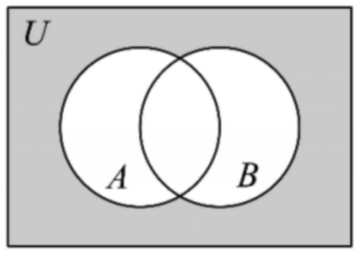
\includegraphics[width=0.20\textwidth]{figures/gao84_q9_venn.png}
\end{center}

\ifanswer
\solbegin
\step{$U=\{1,2,3,4,5,6,7,8,9,10\}$，$A=\{1,2\}$，$B=\{2,4\}$.}
\step{图中阴影部分表示的集合为 $\overline{A\cup B}=\{3,5,6,7,8,9,10\}$，共 $7$ 个元素，}
\step{其非空真子集的个数为 $2^7-2=126$.}
\solend
\fi

\item 若不等式 $ax^2-5x+c<0$ 的解集是 $(2,3)$，则不等式 $cx^2+5x+a\geqslant0$ 的解集是\blankline[4.4em].

\ifanswer
\solbegin
\step{若不等式 $ax^2-5x+c<0$ 的解集是 $(2,3)$，则 $a>0$ 且 $\begin{cases}\dfrac5a=5\\[2pt] \dfrac ca=6\end{cases}$，}
\step{则 $a=1$，$c=6$，}
\step{则不等式 $cx^2+5x+a\geqslant0$ 可化为 $6x^2+5x+1\geqslant0$，则 $x\leqslant-\dfrac12$ 或 $x\geqslant-\dfrac13$，}
\step{则不等式的解集为 $\left(-\infty,-\dfrac12\right]\cup\left[-\dfrac13,+\infty\right)$.}
\solend
\fi

\item 若关于 $x$ 的方程 $mx^2+2x+2=0$ 至少有一个负实根，则实数 $m$ 的取值范围是\blankline[4.4em].

\ifanswer
\solbegin
\step{①当 $m=0$ 时，方程为 $2x+2=0$，有一个负根，满足题意，}
\step{②当 $m\neq0$ 时，关于 $x$ 的方程 $mx^2+2x+2=0$ 至少有一个负根，}
\step{设根为 $x_1$、$x_2$，}
\step{当 $\Delta=4-8m=0$ 时，即 $m=\dfrac12$ 时，方程为 $\dfrac12x^2+2x+1=0$，}
\step{解得 $x=-2$，满足题意，}
\step{当 $\Delta=4-8m>0$，即 $m<\dfrac12$ 时，且 $m\neq0$ 时，}
\step{若有一个负根，则 $x_1x_2=\dfrac2m<0$，解得 $m<0$，}
\step{若有两个负根，则 $\begin{cases}x_1+x_2=-\dfrac2m<0\\[2pt] x_1x_2=\dfrac2m>0\end{cases}$，解得 $0<m<\dfrac12$，}
\step{综上所述，则实数 $m$ 的取值范围是 $\left(-\infty,\dfrac12\right]$.}
\solend
\fi

\item 设集合 $S$、$T$ 都至少含有两个元素，且 $S$、$T$ 同时满足：条件 1：对任意 $x$、$y\in S$，若
$x\neq y$，则 $x+y\in T$；条件 2：对任意 $x$、$y\in T$，若 $x\neq y$，则 $x-y\in S$. 给出下列说法：

①若 $S$ 只有 $2$ 个元素，则这 $2$ 个元素互为相反数；

②若 $S$ 只有 $2$ 个元素，则 $S\cup T$ 必有 $3$ 个元素；

③若 $S$ 只有 $2$ 个元素，则 $S\cup T$ 可能有 $4$ 个元素；

④存在含有 $3$ 个元素的集合 $S$，满足 $S\cup T$ 有 $4$ 个元素.

其中所有正确说法的序号是\blankline[4.4em].

\ifanswer
\solbegin
\step{对于①：由条件 2 得 $x-y\in S$，$y-x\in S$，且 $x-y\neq y-x$，}
\step{所以若 $S$ 只有 $2$ 个元素，则这 $2$ 个元素互为相反数，故①正确；}
\step{对于④：若 $S$ 有 $3$ 个元素，不妨设 $S=\{a,b,c\}$，其中 $a<b<c$，}
\step{则 $\{a+b,b+c,c+a\}\subseteq T$，所以 $c-a$、$c-b$、$b-a$、$a-c$、$b-c$、$a-b\in S$，}
\step{而 $c-a$ 与 $c-b$ 为两个互不相等的正数，$a-c$ 与 $a-b$ 为两个互不相等的负数，}
\step{故集合 $S$ 中至少有 $4$ 个元素，与 $S=\{a,b,c\}$ 有 $3$ 个元素矛盾，故④错误.}
\step{对于②③：若 $S$ 有 $2$ 个元素，由①得集合 $S$ 中的 $2$ 个元素必为相反数，}
\step{故可设 $S=\{a,-a\}(a\neq0)$. 由条件 1 得 $0\in T$，}
\step{由于集合 $T$ 中至少有 $2$ 个元素，故至少还有另外一个元素 $m\in T$.}
\step{当集合 $T$ 只有 $2$ 个元素时即 $T=\{0,m\}$，由条件 1 得 $-m\in S$，则 $m=\pm a$，}
\step{$T=\{0,a\}$ 或 $T=\{0,-a\}$，故 $S\cup T=\{0,a,-a\}$.}
\step{当集合 $T$ 有多于 $2$ 个元素时，不妨设 $T=\{0,m,n\}$，}
\step{则 $m$、$n$、$-m$、$-n$、$m-n$、$n-m\in S$，由于 $m$、$n\neq0$，}
\step{所以 $m\neq m-n$，$n\neq n-m$，又 $m\neq n$，}
\step{故集合 $S$ 至少有 $3$ 个元素，与 $S$ 中只有两个元素矛盾.}
\step{综上，$S\cup T=\{0,a,-a\}$，故②正确，③错误.}
\step{故正确的是①②.}
\solend
\fi

\end{enumerate}

\bigsec{二、选择题}

\begin{enumerate}
\setcounter{enumi}{12}

\item 用反证法证明命题：“若 $x+y>2$，则 $x>1$ 或 $y>1$”时，应假设\mbox{（\quad）}

\keepwithprev
A. $x\leqslant1$ 或 $y\leqslant1$\qquad B. 若 $x>1$ 或 $y>1$

C. $x\leqslant1$ 且 $y\leqslant1$\qquad D. 若 $x>1$ 且 $y>1$

\ifanswer
\ans{$C$}
\fi

\item 下列命题中，为真命题的是\mbox{（\quad）}

\keepwithprev
A. 若 $a>b$，则 $a^2>b^2$\qquad B. 若 $a>b$，$c>d$，则 $ac>bd$

C. 若 $a>b$，则 $\dfrac1a<\dfrac1b$\qquad D. 若 $ac^2>bc^2$，则 $a>b$

\ifanswer
\solbegin
\step{对于 $A$，当 $a=-1$，$b=-2$ 时，$a^2<b^2$，故 $A$ 错误；}
\step{对于 $B$，当 $a=-1$，$b=-2$，$c=-1$，$d=-2$ 时，$ac<bd$，故 $B$ 错误；}
\step{对于 $C$，当 $a=1$，$b=-2$ 时，$\dfrac1a>\dfrac1b$，故 $C$ 错误；}
\step{对于 $D$，因为 $ac^2-bc^2=(a-b)c^2>0$，所以 $a-b>0$，$c^2>0$，则 $a>b$，}
\step{故 $D$ 正确.}
\step{故选 $D$.}
\solend
\fi

\item 现有一级小麦 $m\,\mathrm{kg}$，二级小麦 $n\,\mathrm{kg}$，某粮食收购站有两种收购方案. 方案一：分两个
等级收购小麦，一级小麦 $a$ 元$/\mathrm{kg}$，二级小麦 $b$ 元$/\mathrm{kg}\,(b<a)$；方案二：以方案一两种价
格的平均数收购. 收购方式更加优惠的是\mbox{（\quad）}

\keepwithprev
A. 方案一\qquad B. 方案二\qquad C. 同样优惠\qquad D. 以上均有可能

\ifanswer
\solbegin
\step{方案一收购的平均价格为 $\dfrac{ma+nb}{m+n}$，方案二收购的平均价格为 $\dfrac{a+b}2$；}
\step{所以 $\dfrac{ma+nb}{m+n}-\dfrac{a+b}2=\dfrac{(a-b)(m-n)}{2(m+n)}$ ①，}
\step{$a-b>0$，$m-n$ 的正负性不确定，故①式的正负性不确定，故选 $D$.}
\solend
\fi

\item 用 $C(A)$ 表示非空集合 $A$ 中的元素个数. 对于集合 $A$、$B$，定义

$A*B=\begin{cases}C(A)-C(B),&C(A)\geqslant C(B)\\ C(B)-C(A),&C(A)<C(B)\end{cases}$，若 $A=\{0,1\}$，

$B=\{x\mid(x^2-ax)(x^2+ax+2)=0\}$，设实数 $a$ 的所有可能取值组成的集合是 $S$，则下列选
项不正确的是\mbox{（\quad）}

\keepwithprev
A. $C(B)$ 的可能值为 $1$，$2$，$3$，$4$

B. 若 $A*B=2$，则 $a$ 的取值范围为 $(-\infty,-2\sqrt2)\cup(2\sqrt2,+\infty)$

C. 若 $A*B=1$，则 $C(S)=3$

D. 若 $A*B=0$，则 $a$ 的取值范围为 $(-2\sqrt2,2\sqrt2)$

\ifanswer
\solbegin
\step{对于集合 $B$，当 $a=0$ 时，方程 $x^2(x^2+2)=0$ 的解为 $x=0$，$C(B)=1$，}
\step{当 $a\neq0$ 时，$x^2-ax=0$ 或 $x^2+ax+2=0$，}
\step{其中 $x^2-ax=0$ 的解为 $x_1=0$，$x_2=a$，}
\step{若 $\Delta=a^2-8>0$，即 $a>2\sqrt2$ 或 $a<-2\sqrt2$，}
\step{方程 $x^2+ax+2=0$ 有两个不相等的实数根，此时 $C(B)=4$；}
\step{若 $\Delta=a^2-8=0$，即 $a=2\sqrt2$ 或 $-2\sqrt2$，}
\step{方程 $x^2+ax+2=0$ 有两个相等的实数根，此时 $C(B)=3$；}
\step{若 $\Delta=a^2-8<0$，即 $-2\sqrt2<a<0$ 或 $0<a<2\sqrt2$，}
\step{方程 $x^2+ax+2=0$ 无实数根，此时 $C(B)=2$；}
\step{所以 $C(B)$ 的可能值为 $1$，$2$，$3$，$4$，故 $A$ 正确；}
\step{若 $A*B=2$，且 $C(A)=2$，则 $C(B)=4$，}
\step{则 $a$ 的取值范围 $(-\infty,-2\sqrt2)\cup(2\sqrt2,+\infty)$，故 $B$ 正确；}
\step{若 $A*B=1$，且 $C(A)=2$，则 $C(B)=1$ 或 $3$，}
\step{当 $C(B)=1$ 时，$a=0$，}
\step{当 $C(B)=3$ 时，$a=2\sqrt2$ 或 $-2\sqrt2$，此时集合 $S=\{0,-2\sqrt2,2\sqrt2\}$，}
\step{则 $C(S)=3$，故 $C$ 正确；}
\step{若 $A*B=0$，且 $C(A)=2$，则 $C(B)=2$，}
\step{由此可得 $a$ 的取值范围为 $(-2\sqrt2,0)\cup(0,2\sqrt2)$，故 $D$ 不正确；}
\step{故选 $D$.}
\solend
\fi

\end{enumerate}

\bigsec{三、解答题}

\begin{enumerate}
\setcounter{enumi}{16}

\item 已知集合 $A=\{x\mid-3<x\leqslant4\}$，集合 $B=\{x\mid k+1\leqslant x\leqslant2k-1\}$.

（1）当 $k=3$ 时，求 $A\cup B$、$\overline A\cap B$；

（2）若 $B\subseteq A$，求 $k$ 的取值范围.

\ansspace*[10]

\ifanswer
\solbegin
\stepm{（1）}{当 $k=3$ 时，$B=\{x\mid4\leqslant x\leqslant5\}$，又 $A=\{x\mid-3<x\leqslant4\}$，}
\step{所以 $\overline A=\{x\mid x\leqslant-3$ 或 $x>4\}$，}
\step{所以 $A\cup B=\{x\mid-3<x\leqslant5\}$，$\overline A\cap B=\{x\mid4<x\leqslant5\}$.}
\stepm{（2）}{①当 $B=\varnothing$，即 $k+1>2k-1$ 时，$k<2$，满足 $B\subseteq A$.}
\step{②当 $B\neq\varnothing$ 时，由 $B\subseteq A$ 得 $\begin{cases}k+1\leqslant2k-1\\ k+1>-3\\ 2k-1\leqslant4\end{cases}$，解得 $2\leqslant k\leqslant\dfrac52$，}
\step{综合①②得 $k$ 的取值范围 $\left\{k\mid k\leqslant\dfrac52\right\}$.}
\solend
\fi

\item 设集合 $A=\{x\mid x^2-3x+2=0\}$，$B=\{x\mid x^2+2(a+1)x+a^2-5=0\}$.

（1）若 $A\cap B=\{2\}$，求实数 $a$ 的值；

（2）若集合 $B$ 中有两个元素 $x_1,x_2$，求 $\lvert x_1-x_2\rvert$（用 $a$ 表示）.

\ansspace*[10]

\ifanswer
\solbegin
\stepm{（1）}{由题意得 $A=\{x\mid x^2-3x+2=0\}=\{1,2\}$，因为 $A\cap B=\{2\}$，所以 $2\in B$，}
\step{所以 $2^2+4(a+1)+a^2-5=0$ 即 $4+4a+4+a^2-5=0$，}
\step{化简得 $a^2+4a+3=0$，即 $(a+3)(a+1)=0$，解得 $a=-3$ 或 $a=-1$，}
\step{检验：当 $a=-3$ 时，$B=\{x\mid x^2-4x+4=0\}=\{2\}$，满足 $A\cap B=\{2\}$，}
\step{当 $a=-1$ 时，$B=\{x\mid x^2-4=0\}=\{-2,2\}$，满足 $A\cap B=\{2\}$，}
\step{所以 $a=-3$ 或 $a=-1$.}
\stepm{（2）}{因为 $B$ 中有两个元素 $x_1,x_2$，所以 $x^2+2(a+1)x+(a^2-5)=0$ 有两个根，}
\step{所以 $\Delta=4(a+1)^2-4(a^2-5)=8a+24>0$，}
\step{且 $x_1+x_2=-2(a+1)$，$x_1x_2=a^2-5$，}
\step{所以 $\lvert x_1-x_2\rvert=\sqrt{(x_1+x_2)^2-4x_1x_2}=\sqrt{4(a+1)^2-4(a^2-5)}=\sqrt{8a+24}$.}
\solend
\fi

\item 已知关于 $x$ 的不等式 $\dfrac{ax-2}{1+x}>0$.

（1）若 $x=-a$ 时，不等式成立，求实数 $a$ 的取值范围；

（2）若 $a$ 为实数，解关于 $x$ 的不等式：$\dfrac{ax-2}{1+x}>0$.

\ansspace*[12]

\ifanswer
\solbegin
\stepm{（1）}{因为 $x=-a$ 时，不等式成立，}
\step{所以 $\dfrac{-a^2-2}{1-a}>0\Rightarrow\dfrac{a^2+2}{a-1}>0\Rightarrow a-1>0\Rightarrow a>1$，}
\step{所以实数 $a$ 的取值范围为 $(1,+\infty)$.}
\stepm{（2）}{$\dfrac{ax-2}{1+x}>0\Rightarrow(ax-2)(x+1)>0$，}
\step{当 $a=0$ 时，$-2(x+1)>0$，解得 $x<-1$.}
\step{当 $a>0$ 时，$(ax-2)(x+1)>0$，解得 $x>\dfrac2a$ 或 $x<-1$.}
\step{当 $a<0$ 时，不等式 $(ax-2)(x+1)>0$ 可化为 $\left(x-\dfrac2a\right)(x+1)<0$，}
\step{当 $\dfrac2a>-1$，即 $a<-2$ 时，解得 $-1<x<\dfrac2a$；}
\step{当 $\dfrac2a<-1$，即 $-2<a<0$ 时，解得 $\dfrac2a<x<-1$；}
\step{当 $\dfrac2a=-1$，即 $a=-2$ 时，解集为 $\varnothing$.}
\step{综上，当 $a<-2$ 时，不等式的解集为 $\left(-1,\dfrac2a\right)$；}
\step{当 $a=-2$ 时，不等式的解集为 $\varnothing$；}
\step{当 $-2<a<0$ 时，不等式的解集为 $\left(\dfrac2a,-1\right)$；}
\step{当 $a=0$ 时，不等式的解集为 $(-\infty,-1)$；}
\step{当 $a>0$ 时，不等式的解集为 $(-\infty,-1)\cup\left(\dfrac2a,+\infty\right)$.}
\solend
\fi

\item 已知关于 $x$ 的不等式 $(k^2-2k-3)x^2+(k+1)x+1>0\,(k\in\R)$ 的解集为 $M$；

（1）若存在实数 $a$，使得 $M=(-\infty,a)\cup(a,+\infty)$，求 $k$ 的值；

（2）若 $M=\R$，求 $k$ 的取值范围；

（3）是否存在实数 $k$，满足：“对于任意 $n\in\N$，$n>0$，都有 $n\in M$；对于任意
$m\in\Z$，$m<0$，都有 $m\notin M$”，若存在，求出 $k$ 的值，若不存在，说明理由.

\ansspace*[13]

\ifanswer
\solbegin
\stepm{（1）}{记 $f(x)=(k^2-2k-3)x^2+(k+1)x+1$.}
\step{$M=(-\infty,a)\cup(a,+\infty)$ 表示 $f(x)>0$ 对一切 $x\neq a$ 成立，且 $f(a)=0$，}
\step{故需二次项系数大于 $0$ 且 $\Delta=0$.}
\step{由 $\Delta=(k+1)^2-4(k^2-2k-3)=-3k^2+10k+13=0$ 得 $k=\dfrac{13}3$ 或 $k=-1$.}
\step{当 $k=\dfrac{13}3$ 时，二次项系数 $\dfrac{64}9>0$，$f(x)=\dfrac{64}9\left(x+\dfrac38\right)^2$，符合；}
\step{当 $k=-1$ 时二次项系数为 $0$，$f(x)=1>0$，$M=\R$，不符合. 故 $k=\dfrac{13}3$.}
\stepm{（2）}{$M=\R$ 即 $f(x)>0$ 对一切 $x\in\R$ 恒成立.}
\step{①当 $k^2-2k-3>0$（即 $k<-1$ 或 $k>3$）时，需 $\Delta<0$，}
\step{即 $-3k^2+10k+13<0$，得 $k<-1$ 或 $k>\dfrac{13}3$，故 $k<-1$ 或 $k>\dfrac{13}3$；}
\step{②当 $k^2-2k-3=0$ 时，$k=3$ 得 $f(x)=4x+1$ 不恒正，不符合题意，}
\step{舍去，}
\step{当 $k=-1$ 得 $f(x)=1>0$ 恒成立，符合题意；}
\step{③当 $k^2-2k-3<0$ 时，抛物线开口向下，不能恒正.}
\step{综上，$k\leqslant-1$ 或 $k>\dfrac{13}3$.}
\stepm{（3）}{存在，$k=3$，理由如下，}
\step{由题意得解集 $M=(t,+\infty)$，$t\in[-1,1)$；}
\step{当 $k^2-2k-3=0$ 时，解得 $k=3$ 或 $k=-1$，}
\step{$k=3$ 时，不等式的解集为 $\left(-\dfrac14,+\infty\right)$，满足条件；}
\step{$k=-1$ 时，$1>0$ 恒成立，不满足条件；}
\step{当 $k^2-2k-3>0$ 时，}
\step{此时对应的一元二次不等式的解集形式不是 $(t,+\infty)$ 的形式，不满足条件；}
\step{当 $k^2-2k-3<0$ 时，}
\step{此时对应的一元二次不等式的解集形式不是 $(t,+\infty)$ 的形式，不满足条件；}
\step{综上，满足条件 $k$ 的值为 $3$.}
\solend
\fi

\item 已知有限集 $A=\{a_1,a_2,\cdots,a_n\}\,(n\geqslant2,n\in\N)$，如果 $A$ 中元素 $a_i\,(i=1,2,3,\cdots,n)$ 满足
$a_1+a_2+a_3+\cdots+a_n=a_1\times a_2\times\cdots\times a_n$，就称 $A$ 为“和积平衡集”.

（1）判断集合 $\{-1+\sqrt3,-1-\sqrt3\}$ 是否为“和积平衡集”；

（2）若 $a_1$、$a_2$ 是两个不同的正数，且 $\{a_1,a_2\}$ 是“和积平衡集”，写出以 $a_1$、$a_2$ 为根的一
个一元二次方程（系数可用 $a_1$、$a_2$ 表示），并证明 $a_1$、$a_2$ 至少有一个大于 $2$；

（3）若 $a_i\in\Z$ 且 $a_i>0$，求所有符合条件的“和积平衡集”.

\ansspace*[14]

\ifanswer
\solbegin
\stepm{（1）}{对于集合 $\{-1+\sqrt3,-1-\sqrt3\}$，}
\step{因为 $(-1+\sqrt3)+(-1-\sqrt3)=-2$，$(-1+\sqrt3)\times(-1-\sqrt3)=-2$，}
\step{所以满足 $a_1+a_2=a_1\times a_2$，满足题意，}
\step{所以集合 $\{-1+\sqrt3,-1-\sqrt3\}$ 是和积平衡集.}
\stepm{（2）}{以 $a_1$、$a_2$ 为根的一个一元二次方程可为 $x^2-(a_1+a_2)x+a_1\cdot a_2=0$，}
\step{因为 $a_1$、$a_2$ 是两个不同的正数，且 $\{a_1,a_2\}$ 是和积平衡集，}
\step{所以 $a_1+a_2=a_1\cdot a_2$，}
\step{又 $a_1$ 和 $a_2$ 为 $x^2-(a_1+a_2)x+a_1\cdot a_2=0$ 的两个不同的正根，}
\step{所以 $\Delta=(a_1+a_2)^2-4a_1a_2=(a_1+a_2)^2-4(a_1+a_2)>0$，}
\step{又 $a_1+a_2>0$，则 $a_1+a_2>4$，}
\step{若 $a_1$、$a_2$ 都小于等于 $2$，则 $a_1+a_2\leqslant4$，矛盾，}
\step{所以 $a_1$、$a_2$ 至少有一个大于 $2$；}
\stepm{（3）}{设 $A$ 中的 $a_1<a_2<a_3<\cdots<a_n$，且 $a_i\in\N^*$，}
\step{由 $a_1+a_2+a_3+\cdots+a_n=a_1\times a_2\times\cdots\times a_n$，得 $n=2$ 时明显不满足，}
\step{所以 $n\geqslant3$，故 $a_1\times a_2\times\cdots\times a_n=a_1+a_2+a_3+\cdots+a_n\leqslant na_n$，}
\step{所以 $a_1\times a_2\times\cdots\times a_{n-1}\leqslant n$，}
\step{当 $n=3$ 时，$a_1\times a_2\leqslant3$，$a_i\in\N^*$，只能有 $a_1=1$，$a_2=2$，}
\step{由 $a_1+a_2+a_3=a_1\times a_2\times a_3$，得 $a_3=3$，此时的和积平衡集为 $\{1,2,3\}$，}
\step{当 $n\geqslant4$ 时，$a_1\times a_2\times\cdots\times a_{n-1}\geqslant(n-1)(n-2)\times\cdots\times2\times1\geqslant(n-1)(n-2)$，}
\step{又 $(n-1)(n-2)-n=n^2-4n+2=n(n-4)+2>0$，即 $(n-1)(n-2)>n$，}
\step{即 $a_1\times a_2\times\cdots\times a_{n-1}>n$，与 $a_1\times a_2\times\cdots\times a_{n-1}\leqslant n$ 矛盾，}
\step{所以 $n\geqslant4$ 不满足条件，}
\step{所以符合条件的和积平衡集有且只有 $n=3$，此时的和积平衡集为 $\{1,2,3\}$.}
\solend
\fi

\end{enumerate}

\end{document}
"
% 紧凑版：xelatex "\def\iscompact{1}% 高一84_东昌中学_10月月考.tex
%   —— 高一上数学“2026-2027 年东昌中学高一上 10 月月考”（讲评版）
% 试卷版：xelatex 高一84_东昌中学_10月月考.tex
% 答案版：xelatex "\def\isanswer{1}% 高一84_东昌中学_10月月考.tex
%   —— 高一上数学“2026-2027 年东昌中学高一上 10 月月考”（讲评版）
% 试卷版：xelatex 高一84_东昌中学_10月月考.tex
% 答案版：xelatex "\def\isanswer{1}\input{高一84_东昌中学_10月月考.tex}"
% 紧凑版：xelatex "\def\iscompact{1}\input{高一84_东昌中学_10月月考.tex}"
%
% 原始材料：微信公众号“魔都数学加油站”文章，连载“27学年高一84”；
% 原文标题“27学年高一84——2026-2027年上海市东昌中学高一上10月月考”；
% 原文链接：https://mp.weixin.qq.com/s/PErsjO3N5RsMuJC69IGbrw。
% 页面标注发布时间 2026-10-26 20:15（上海）。
% 正文为 12 张 PNG 页（`原图/高一84_东昌中学_10月月考/01..12.png`），
% 尺寸混排（第 1—8 页为 4762×6735，第 9—12 页为 2560×3620），均按页序读取。
%
% 篇幅与题号：原卷自第 3 题起编号（第 1、2 题不在原文内）。填空题 3—12（10 题）、
% 选择题 13—16（4 题）、解答题 17—21（5 题），共 19 题。
%
% 讲评版：19 题全部印【解析】，本稿不另提 \ans{}；选择题答案在解析末句“故选 D／C／D”。
% 第 13 题的答案“C”原卷直接印在题干括号内（“（\ C\ ）”），本稿按 高一37 第 13 题／
% 高一63 第 14 题成例括号留空、另提 \ans{$C$}（该题无【解析】段）。
%
% 副标题：原卷未印副标题。本稿按内容标作“集合与常用逻辑用语、不等式”。
%
% 与原卷的排版差异：
%   ① 原卷每题下直接印【解析】，本稿按全稿惯例将解析置于答案版；
%   ② 原卷未印副标题，本稿补出；填空横线统一排 \blankline[4.4em]；
%   ③ 原卷数集记号排斜体 $R$、$Z$、$N$，本稿按全稿惯例改用 $\R$、$\Z$、$\N$；
%   ④ 第 17—21 题的子问用行内“（1）（2）（3）”段，解析中的子问标号用 \stepm；
%   ⑤ 解答题按惯例加 \ansspace；选择题括号排 \mbox{（\quad）}；
%   ⑥ 第 9 题题干右侧有一幅韦恩图，裁自原图（第 2 页）后去粉色水印、转灰度，
%      三版都出（属题干）。
%
% 行数核对：逐题数 \step/\stepm 条数，合计 157 条（Q3：2；Q4：2；Q5：3；Q6：2；
% Q7：3；Q8：6；Q9：3；Q10：4；Q11：9；Q12：17；Q14：6；Q15：3；Q16：19；
% Q17：6；Q18：10；Q19：15；Q20：24；Q21：23）；第 13 题无解析，只提 \ans{}，
% 不计入 \step 账。原卷解析的换行按语意合并，未逐行强拆。
%
\documentclass[a4paper,11pt]{article}
\usepackage{common}

\begin{document}

\examtitlest[4]{2026--2027 年东昌中学高一上 10 月月考}{集合与常用逻辑用语、不等式}

\bigsec{一、填空题}

\begin{enumerate}
\setcounter{enumi}{2}

\item 若 $a\in\R$，则“$a=2$”是“$(a-1)(a-2)=0$”的\blankline[3.6em]条件（填“充分不必要”、“必要
不充分”、“充要”、“既不充分又不必要”的一个）.

\ifanswer
\solbegin
\step{$a=2\Rightarrow(a-1)(a-2)=0$，而 $(a-1)(a-2)=0$ 不能推出 $a=2$，}
\step{故“$a=2$”是“$(a-1)(a-2)=0$”的充分不必要条件.}
\solend
\fi

\item 已知集合 $M=\{(x,y)\mid y=x^2\}$，$N=\{(x,y)\mid y=1\}$，则 $M\cap N=\blankline[4.4em]$.

\ifanswer
\solbegin
\step{集合 $M=\{(x,y)\mid y=x^2\}$，$N=\{(x,y)\mid y=1\}$，}
\step{当 $y=1$ 时，$x=\pm1$，则 $M\cap N=\{(-1,1),(1,1)\}$.}
\solend
\fi

\item 已知集合 $A=\{x\mid x^2+ax+4=0\}$，若 $A$ 有且只有一个非空子集，则实数 $a=\blankline[4.4em]$.

\ifanswer
\solbegin
\step{因为集合 $A$ 有且只有一个非空子集，所以集合 $A$ 中只有一个元素，}
\step{所以一元二次方程 $x^2+ax+4=0$ 有两个相等的解，}
\step{所以 $\Delta=a^2-4\times4=0$，解得 $a=\pm4$.}
\solend
\fi

\item 已知 $A=(-\infty,a]$，$B=(-\infty,3)$，且 $x\in A$ 是 $x\in B$ 的充分不必要条件，则 $a$ 的取值范围
是\blankline[4.4em].

\ifanswer
\solbegin
\step{$A=(-\infty,a]$，$B=(-\infty,3)$，且 $x\in A$ 是 $x\in B$ 的充分不必要条件，}
\step{则 $A\subset B$，则 $a<3$，即 $a$ 的取值范围为 $(-\infty,3)$.}
\solend
\fi

\item 不等式 $\dfrac{3x-1}{x-2}\leqslant1$ 的解集为\blankline[4.4em].

\ifanswer
\solbegin
\step{由 $\dfrac{3x-1}{x-2}\leqslant1$，得 $\dfrac{3x-1}{x-2}-1=\dfrac{3x-1-(x-2)}{x-2}=\dfrac{2x+1}{x-2}\leqslant0$，}
\step{则 $\begin{cases}(2x+1)(x-2)\leqslant0\\ x-2\neq0\end{cases}$，解得 $-\dfrac12\leqslant x<2$，}
\step{则不等式 $\dfrac{3x-1}{x-2}\leqslant1$ 的解集为 $\left[-\dfrac12,2\right)$.}
\solend
\fi

\item 已知关于 $x$ 的一元二次方程 $x^2-2mx+(3m+1)=0$ 的两个实数根为 $x_1$、$x_2$，且
$x_1^2+x_2^2=16$，则实数 $m$ 的值为\blankline[4.4em].

\ifanswer
\solbegin
\step{由韦达定理，得 $x_1+x_2=2m$，$x_1x_2=3m+1$，}
\step{$x_1^2+x_2^2=(x_1+x_2)^2-2x_1x_2=4m^2-6m-2$，}
\step{由 $x_1^2+x_2^2=16$，得 $4m^2-6m-2=16$，即 $2m^2-3m-9=0$，}
\step{解得 $m=3$ 或 $m=-\dfrac32$，}
\step{检验判别式 $\Delta=4m^2-12m-4$，当 $m=3$ 时，$\Delta=-4<0$，舍去；}
\step{当 $m=-\dfrac32$ 时，$\Delta=23>0$，符合条件，故 $m=-\dfrac32$.}
\solend
\fi

\item 已知全集 $U=\{x\mid1\leqslant x\leqslant10,\,x\in\N\}$，集合 $A=\{x\mid x^2-3<4,\,x\in\N,\,x>0\}$，
$B=\{2,4\}$，则图中阴影部分表示的集合的非空真子集个数为\blankline[4.4em].

\needvspace{9\baselineskip}
\begin{center}
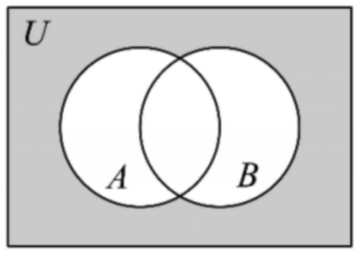
\includegraphics[width=0.20\textwidth]{figures/gao84_q9_venn.png}
\end{center}

\ifanswer
\solbegin
\step{$U=\{1,2,3,4,5,6,7,8,9,10\}$，$A=\{1,2\}$，$B=\{2,4\}$.}
\step{图中阴影部分表示的集合为 $\overline{A\cup B}=\{3,5,6,7,8,9,10\}$，共 $7$ 个元素，}
\step{其非空真子集的个数为 $2^7-2=126$.}
\solend
\fi

\item 若不等式 $ax^2-5x+c<0$ 的解集是 $(2,3)$，则不等式 $cx^2+5x+a\geqslant0$ 的解集是\blankline[4.4em].

\ifanswer
\solbegin
\step{若不等式 $ax^2-5x+c<0$ 的解集是 $(2,3)$，则 $a>0$ 且 $\begin{cases}\dfrac5a=5\\[2pt] \dfrac ca=6\end{cases}$，}
\step{则 $a=1$，$c=6$，}
\step{则不等式 $cx^2+5x+a\geqslant0$ 可化为 $6x^2+5x+1\geqslant0$，则 $x\leqslant-\dfrac12$ 或 $x\geqslant-\dfrac13$，}
\step{则不等式的解集为 $\left(-\infty,-\dfrac12\right]\cup\left[-\dfrac13,+\infty\right)$.}
\solend
\fi

\item 若关于 $x$ 的方程 $mx^2+2x+2=0$ 至少有一个负实根，则实数 $m$ 的取值范围是\blankline[4.4em].

\ifanswer
\solbegin
\step{①当 $m=0$ 时，方程为 $2x+2=0$，有一个负根，满足题意，}
\step{②当 $m\neq0$ 时，关于 $x$ 的方程 $mx^2+2x+2=0$ 至少有一个负根，}
\step{设根为 $x_1$、$x_2$，}
\step{当 $\Delta=4-8m=0$ 时，即 $m=\dfrac12$ 时，方程为 $\dfrac12x^2+2x+1=0$，}
\step{解得 $x=-2$，满足题意，}
\step{当 $\Delta=4-8m>0$，即 $m<\dfrac12$ 时，且 $m\neq0$ 时，}
\step{若有一个负根，则 $x_1x_2=\dfrac2m<0$，解得 $m<0$，}
\step{若有两个负根，则 $\begin{cases}x_1+x_2=-\dfrac2m<0\\[2pt] x_1x_2=\dfrac2m>0\end{cases}$，解得 $0<m<\dfrac12$，}
\step{综上所述，则实数 $m$ 的取值范围是 $\left(-\infty,\dfrac12\right]$.}
\solend
\fi

\item 设集合 $S$、$T$ 都至少含有两个元素，且 $S$、$T$ 同时满足：条件 1：对任意 $x$、$y\in S$，若
$x\neq y$，则 $x+y\in T$；条件 2：对任意 $x$、$y\in T$，若 $x\neq y$，则 $x-y\in S$. 给出下列说法：

①若 $S$ 只有 $2$ 个元素，则这 $2$ 个元素互为相反数；

②若 $S$ 只有 $2$ 个元素，则 $S\cup T$ 必有 $3$ 个元素；

③若 $S$ 只有 $2$ 个元素，则 $S\cup T$ 可能有 $4$ 个元素；

④存在含有 $3$ 个元素的集合 $S$，满足 $S\cup T$ 有 $4$ 个元素.

其中所有正确说法的序号是\blankline[4.4em].

\ifanswer
\solbegin
\step{对于①：由条件 2 得 $x-y\in S$，$y-x\in S$，且 $x-y\neq y-x$，}
\step{所以若 $S$ 只有 $2$ 个元素，则这 $2$ 个元素互为相反数，故①正确；}
\step{对于④：若 $S$ 有 $3$ 个元素，不妨设 $S=\{a,b,c\}$，其中 $a<b<c$，}
\step{则 $\{a+b,b+c,c+a\}\subseteq T$，所以 $c-a$、$c-b$、$b-a$、$a-c$、$b-c$、$a-b\in S$，}
\step{而 $c-a$ 与 $c-b$ 为两个互不相等的正数，$a-c$ 与 $a-b$ 为两个互不相等的负数，}
\step{故集合 $S$ 中至少有 $4$ 个元素，与 $S=\{a,b,c\}$ 有 $3$ 个元素矛盾，故④错误.}
\step{对于②③：若 $S$ 有 $2$ 个元素，由①得集合 $S$ 中的 $2$ 个元素必为相反数，}
\step{故可设 $S=\{a,-a\}(a\neq0)$. 由条件 1 得 $0\in T$，}
\step{由于集合 $T$ 中至少有 $2$ 个元素，故至少还有另外一个元素 $m\in T$.}
\step{当集合 $T$ 只有 $2$ 个元素时即 $T=\{0,m\}$，由条件 1 得 $-m\in S$，则 $m=\pm a$，}
\step{$T=\{0,a\}$ 或 $T=\{0,-a\}$，故 $S\cup T=\{0,a,-a\}$.}
\step{当集合 $T$ 有多于 $2$ 个元素时，不妨设 $T=\{0,m,n\}$，}
\step{则 $m$、$n$、$-m$、$-n$、$m-n$、$n-m\in S$，由于 $m$、$n\neq0$，}
\step{所以 $m\neq m-n$，$n\neq n-m$，又 $m\neq n$，}
\step{故集合 $S$ 至少有 $3$ 个元素，与 $S$ 中只有两个元素矛盾.}
\step{综上，$S\cup T=\{0,a,-a\}$，故②正确，③错误.}
\step{故正确的是①②.}
\solend
\fi

\end{enumerate}

\bigsec{二、选择题}

\begin{enumerate}
\setcounter{enumi}{12}

\item 用反证法证明命题：“若 $x+y>2$，则 $x>1$ 或 $y>1$”时，应假设\mbox{（\quad）}

\keepwithprev
A. $x\leqslant1$ 或 $y\leqslant1$\qquad B. 若 $x>1$ 或 $y>1$

C. $x\leqslant1$ 且 $y\leqslant1$\qquad D. 若 $x>1$ 且 $y>1$

\ifanswer
\ans{$C$}
\fi

\item 下列命题中，为真命题的是\mbox{（\quad）}

\keepwithprev
A. 若 $a>b$，则 $a^2>b^2$\qquad B. 若 $a>b$，$c>d$，则 $ac>bd$

C. 若 $a>b$，则 $\dfrac1a<\dfrac1b$\qquad D. 若 $ac^2>bc^2$，则 $a>b$

\ifanswer
\solbegin
\step{对于 $A$，当 $a=-1$，$b=-2$ 时，$a^2<b^2$，故 $A$ 错误；}
\step{对于 $B$，当 $a=-1$，$b=-2$，$c=-1$，$d=-2$ 时，$ac<bd$，故 $B$ 错误；}
\step{对于 $C$，当 $a=1$，$b=-2$ 时，$\dfrac1a>\dfrac1b$，故 $C$ 错误；}
\step{对于 $D$，因为 $ac^2-bc^2=(a-b)c^2>0$，所以 $a-b>0$，$c^2>0$，则 $a>b$，}
\step{故 $D$ 正确.}
\step{故选 $D$.}
\solend
\fi

\item 现有一级小麦 $m\,\mathrm{kg}$，二级小麦 $n\,\mathrm{kg}$，某粮食收购站有两种收购方案. 方案一：分两个
等级收购小麦，一级小麦 $a$ 元$/\mathrm{kg}$，二级小麦 $b$ 元$/\mathrm{kg}\,(b<a)$；方案二：以方案一两种价
格的平均数收购. 收购方式更加优惠的是\mbox{（\quad）}

\keepwithprev
A. 方案一\qquad B. 方案二\qquad C. 同样优惠\qquad D. 以上均有可能

\ifanswer
\solbegin
\step{方案一收购的平均价格为 $\dfrac{ma+nb}{m+n}$，方案二收购的平均价格为 $\dfrac{a+b}2$；}
\step{所以 $\dfrac{ma+nb}{m+n}-\dfrac{a+b}2=\dfrac{(a-b)(m-n)}{2(m+n)}$ ①，}
\step{$a-b>0$，$m-n$ 的正负性不确定，故①式的正负性不确定，故选 $D$.}
\solend
\fi

\item 用 $C(A)$ 表示非空集合 $A$ 中的元素个数. 对于集合 $A$、$B$，定义

$A*B=\begin{cases}C(A)-C(B),&C(A)\geqslant C(B)\\ C(B)-C(A),&C(A)<C(B)\end{cases}$，若 $A=\{0,1\}$，

$B=\{x\mid(x^2-ax)(x^2+ax+2)=0\}$，设实数 $a$ 的所有可能取值组成的集合是 $S$，则下列选
项不正确的是\mbox{（\quad）}

\keepwithprev
A. $C(B)$ 的可能值为 $1$，$2$，$3$，$4$

B. 若 $A*B=2$，则 $a$ 的取值范围为 $(-\infty,-2\sqrt2)\cup(2\sqrt2,+\infty)$

C. 若 $A*B=1$，则 $C(S)=3$

D. 若 $A*B=0$，则 $a$ 的取值范围为 $(-2\sqrt2,2\sqrt2)$

\ifanswer
\solbegin
\step{对于集合 $B$，当 $a=0$ 时，方程 $x^2(x^2+2)=0$ 的解为 $x=0$，$C(B)=1$，}
\step{当 $a\neq0$ 时，$x^2-ax=0$ 或 $x^2+ax+2=0$，}
\step{其中 $x^2-ax=0$ 的解为 $x_1=0$，$x_2=a$，}
\step{若 $\Delta=a^2-8>0$，即 $a>2\sqrt2$ 或 $a<-2\sqrt2$，}
\step{方程 $x^2+ax+2=0$ 有两个不相等的实数根，此时 $C(B)=4$；}
\step{若 $\Delta=a^2-8=0$，即 $a=2\sqrt2$ 或 $-2\sqrt2$，}
\step{方程 $x^2+ax+2=0$ 有两个相等的实数根，此时 $C(B)=3$；}
\step{若 $\Delta=a^2-8<0$，即 $-2\sqrt2<a<0$ 或 $0<a<2\sqrt2$，}
\step{方程 $x^2+ax+2=0$ 无实数根，此时 $C(B)=2$；}
\step{所以 $C(B)$ 的可能值为 $1$，$2$，$3$，$4$，故 $A$ 正确；}
\step{若 $A*B=2$，且 $C(A)=2$，则 $C(B)=4$，}
\step{则 $a$ 的取值范围 $(-\infty,-2\sqrt2)\cup(2\sqrt2,+\infty)$，故 $B$ 正确；}
\step{若 $A*B=1$，且 $C(A)=2$，则 $C(B)=1$ 或 $3$，}
\step{当 $C(B)=1$ 时，$a=0$，}
\step{当 $C(B)=3$ 时，$a=2\sqrt2$ 或 $-2\sqrt2$，此时集合 $S=\{0,-2\sqrt2,2\sqrt2\}$，}
\step{则 $C(S)=3$，故 $C$ 正确；}
\step{若 $A*B=0$，且 $C(A)=2$，则 $C(B)=2$，}
\step{由此可得 $a$ 的取值范围为 $(-2\sqrt2,0)\cup(0,2\sqrt2)$，故 $D$ 不正确；}
\step{故选 $D$.}
\solend
\fi

\end{enumerate}

\bigsec{三、解答题}

\begin{enumerate}
\setcounter{enumi}{16}

\item 已知集合 $A=\{x\mid-3<x\leqslant4\}$，集合 $B=\{x\mid k+1\leqslant x\leqslant2k-1\}$.

（1）当 $k=3$ 时，求 $A\cup B$、$\overline A\cap B$；

（2）若 $B\subseteq A$，求 $k$ 的取值范围.

\ansspace*[10]

\ifanswer
\solbegin
\stepm{（1）}{当 $k=3$ 时，$B=\{x\mid4\leqslant x\leqslant5\}$，又 $A=\{x\mid-3<x\leqslant4\}$，}
\step{所以 $\overline A=\{x\mid x\leqslant-3$ 或 $x>4\}$，}
\step{所以 $A\cup B=\{x\mid-3<x\leqslant5\}$，$\overline A\cap B=\{x\mid4<x\leqslant5\}$.}
\stepm{（2）}{①当 $B=\varnothing$，即 $k+1>2k-1$ 时，$k<2$，满足 $B\subseteq A$.}
\step{②当 $B\neq\varnothing$ 时，由 $B\subseteq A$ 得 $\begin{cases}k+1\leqslant2k-1\\ k+1>-3\\ 2k-1\leqslant4\end{cases}$，解得 $2\leqslant k\leqslant\dfrac52$，}
\step{综合①②得 $k$ 的取值范围 $\left\{k\mid k\leqslant\dfrac52\right\}$.}
\solend
\fi

\item 设集合 $A=\{x\mid x^2-3x+2=0\}$，$B=\{x\mid x^2+2(a+1)x+a^2-5=0\}$.

（1）若 $A\cap B=\{2\}$，求实数 $a$ 的值；

（2）若集合 $B$ 中有两个元素 $x_1,x_2$，求 $\lvert x_1-x_2\rvert$（用 $a$ 表示）.

\ansspace*[10]

\ifanswer
\solbegin
\stepm{（1）}{由题意得 $A=\{x\mid x^2-3x+2=0\}=\{1,2\}$，因为 $A\cap B=\{2\}$，所以 $2\in B$，}
\step{所以 $2^2+4(a+1)+a^2-5=0$ 即 $4+4a+4+a^2-5=0$，}
\step{化简得 $a^2+4a+3=0$，即 $(a+3)(a+1)=0$，解得 $a=-3$ 或 $a=-1$，}
\step{检验：当 $a=-3$ 时，$B=\{x\mid x^2-4x+4=0\}=\{2\}$，满足 $A\cap B=\{2\}$，}
\step{当 $a=-1$ 时，$B=\{x\mid x^2-4=0\}=\{-2,2\}$，满足 $A\cap B=\{2\}$，}
\step{所以 $a=-3$ 或 $a=-1$.}
\stepm{（2）}{因为 $B$ 中有两个元素 $x_1,x_2$，所以 $x^2+2(a+1)x+(a^2-5)=0$ 有两个根，}
\step{所以 $\Delta=4(a+1)^2-4(a^2-5)=8a+24>0$，}
\step{且 $x_1+x_2=-2(a+1)$，$x_1x_2=a^2-5$，}
\step{所以 $\lvert x_1-x_2\rvert=\sqrt{(x_1+x_2)^2-4x_1x_2}=\sqrt{4(a+1)^2-4(a^2-5)}=\sqrt{8a+24}$.}
\solend
\fi

\item 已知关于 $x$ 的不等式 $\dfrac{ax-2}{1+x}>0$.

（1）若 $x=-a$ 时，不等式成立，求实数 $a$ 的取值范围；

（2）若 $a$ 为实数，解关于 $x$ 的不等式：$\dfrac{ax-2}{1+x}>0$.

\ansspace*[12]

\ifanswer
\solbegin
\stepm{（1）}{因为 $x=-a$ 时，不等式成立，}
\step{所以 $\dfrac{-a^2-2}{1-a}>0\Rightarrow\dfrac{a^2+2}{a-1}>0\Rightarrow a-1>0\Rightarrow a>1$，}
\step{所以实数 $a$ 的取值范围为 $(1,+\infty)$.}
\stepm{（2）}{$\dfrac{ax-2}{1+x}>0\Rightarrow(ax-2)(x+1)>0$，}
\step{当 $a=0$ 时，$-2(x+1)>0$，解得 $x<-1$.}
\step{当 $a>0$ 时，$(ax-2)(x+1)>0$，解得 $x>\dfrac2a$ 或 $x<-1$.}
\step{当 $a<0$ 时，不等式 $(ax-2)(x+1)>0$ 可化为 $\left(x-\dfrac2a\right)(x+1)<0$，}
\step{当 $\dfrac2a>-1$，即 $a<-2$ 时，解得 $-1<x<\dfrac2a$；}
\step{当 $\dfrac2a<-1$，即 $-2<a<0$ 时，解得 $\dfrac2a<x<-1$；}
\step{当 $\dfrac2a=-1$，即 $a=-2$ 时，解集为 $\varnothing$.}
\step{综上，当 $a<-2$ 时，不等式的解集为 $\left(-1,\dfrac2a\right)$；}
\step{当 $a=-2$ 时，不等式的解集为 $\varnothing$；}
\step{当 $-2<a<0$ 时，不等式的解集为 $\left(\dfrac2a,-1\right)$；}
\step{当 $a=0$ 时，不等式的解集为 $(-\infty,-1)$；}
\step{当 $a>0$ 时，不等式的解集为 $(-\infty,-1)\cup\left(\dfrac2a,+\infty\right)$.}
\solend
\fi

\item 已知关于 $x$ 的不等式 $(k^2-2k-3)x^2+(k+1)x+1>0\,(k\in\R)$ 的解集为 $M$；

（1）若存在实数 $a$，使得 $M=(-\infty,a)\cup(a,+\infty)$，求 $k$ 的值；

（2）若 $M=\R$，求 $k$ 的取值范围；

（3）是否存在实数 $k$，满足：“对于任意 $n\in\N$，$n>0$，都有 $n\in M$；对于任意
$m\in\Z$，$m<0$，都有 $m\notin M$”，若存在，求出 $k$ 的值，若不存在，说明理由.

\ansspace*[13]

\ifanswer
\solbegin
\stepm{（1）}{记 $f(x)=(k^2-2k-3)x^2+(k+1)x+1$.}
\step{$M=(-\infty,a)\cup(a,+\infty)$ 表示 $f(x)>0$ 对一切 $x\neq a$ 成立，且 $f(a)=0$，}
\step{故需二次项系数大于 $0$ 且 $\Delta=0$.}
\step{由 $\Delta=(k+1)^2-4(k^2-2k-3)=-3k^2+10k+13=0$ 得 $k=\dfrac{13}3$ 或 $k=-1$.}
\step{当 $k=\dfrac{13}3$ 时，二次项系数 $\dfrac{64}9>0$，$f(x)=\dfrac{64}9\left(x+\dfrac38\right)^2$，符合；}
\step{当 $k=-1$ 时二次项系数为 $0$，$f(x)=1>0$，$M=\R$，不符合. 故 $k=\dfrac{13}3$.}
\stepm{（2）}{$M=\R$ 即 $f(x)>0$ 对一切 $x\in\R$ 恒成立.}
\step{①当 $k^2-2k-3>0$（即 $k<-1$ 或 $k>3$）时，需 $\Delta<0$，}
\step{即 $-3k^2+10k+13<0$，得 $k<-1$ 或 $k>\dfrac{13}3$，故 $k<-1$ 或 $k>\dfrac{13}3$；}
\step{②当 $k^2-2k-3=0$ 时，$k=3$ 得 $f(x)=4x+1$ 不恒正，不符合题意，}
\step{舍去，}
\step{当 $k=-1$ 得 $f(x)=1>0$ 恒成立，符合题意；}
\step{③当 $k^2-2k-3<0$ 时，抛物线开口向下，不能恒正.}
\step{综上，$k\leqslant-1$ 或 $k>\dfrac{13}3$.}
\stepm{（3）}{存在，$k=3$，理由如下，}
\step{由题意得解集 $M=(t,+\infty)$，$t\in[-1,1)$；}
\step{当 $k^2-2k-3=0$ 时，解得 $k=3$ 或 $k=-1$，}
\step{$k=3$ 时，不等式的解集为 $\left(-\dfrac14,+\infty\right)$，满足条件；}
\step{$k=-1$ 时，$1>0$ 恒成立，不满足条件；}
\step{当 $k^2-2k-3>0$ 时，}
\step{此时对应的一元二次不等式的解集形式不是 $(t,+\infty)$ 的形式，不满足条件；}
\step{当 $k^2-2k-3<0$ 时，}
\step{此时对应的一元二次不等式的解集形式不是 $(t,+\infty)$ 的形式，不满足条件；}
\step{综上，满足条件 $k$ 的值为 $3$.}
\solend
\fi

\item 已知有限集 $A=\{a_1,a_2,\cdots,a_n\}\,(n\geqslant2,n\in\N)$，如果 $A$ 中元素 $a_i\,(i=1,2,3,\cdots,n)$ 满足
$a_1+a_2+a_3+\cdots+a_n=a_1\times a_2\times\cdots\times a_n$，就称 $A$ 为“和积平衡集”.

（1）判断集合 $\{-1+\sqrt3,-1-\sqrt3\}$ 是否为“和积平衡集”；

（2）若 $a_1$、$a_2$ 是两个不同的正数，且 $\{a_1,a_2\}$ 是“和积平衡集”，写出以 $a_1$、$a_2$ 为根的一
个一元二次方程（系数可用 $a_1$、$a_2$ 表示），并证明 $a_1$、$a_2$ 至少有一个大于 $2$；

（3）若 $a_i\in\Z$ 且 $a_i>0$，求所有符合条件的“和积平衡集”.

\ansspace*[14]

\ifanswer
\solbegin
\stepm{（1）}{对于集合 $\{-1+\sqrt3,-1-\sqrt3\}$，}
\step{因为 $(-1+\sqrt3)+(-1-\sqrt3)=-2$，$(-1+\sqrt3)\times(-1-\sqrt3)=-2$，}
\step{所以满足 $a_1+a_2=a_1\times a_2$，满足题意，}
\step{所以集合 $\{-1+\sqrt3,-1-\sqrt3\}$ 是和积平衡集.}
\stepm{（2）}{以 $a_1$、$a_2$ 为根的一个一元二次方程可为 $x^2-(a_1+a_2)x+a_1\cdot a_2=0$，}
\step{因为 $a_1$、$a_2$ 是两个不同的正数，且 $\{a_1,a_2\}$ 是和积平衡集，}
\step{所以 $a_1+a_2=a_1\cdot a_2$，}
\step{又 $a_1$ 和 $a_2$ 为 $x^2-(a_1+a_2)x+a_1\cdot a_2=0$ 的两个不同的正根，}
\step{所以 $\Delta=(a_1+a_2)^2-4a_1a_2=(a_1+a_2)^2-4(a_1+a_2)>0$，}
\step{又 $a_1+a_2>0$，则 $a_1+a_2>4$，}
\step{若 $a_1$、$a_2$ 都小于等于 $2$，则 $a_1+a_2\leqslant4$，矛盾，}
\step{所以 $a_1$、$a_2$ 至少有一个大于 $2$；}
\stepm{（3）}{设 $A$ 中的 $a_1<a_2<a_3<\cdots<a_n$，且 $a_i\in\N^*$，}
\step{由 $a_1+a_2+a_3+\cdots+a_n=a_1\times a_2\times\cdots\times a_n$，得 $n=2$ 时明显不满足，}
\step{所以 $n\geqslant3$，故 $a_1\times a_2\times\cdots\times a_n=a_1+a_2+a_3+\cdots+a_n\leqslant na_n$，}
\step{所以 $a_1\times a_2\times\cdots\times a_{n-1}\leqslant n$，}
\step{当 $n=3$ 时，$a_1\times a_2\leqslant3$，$a_i\in\N^*$，只能有 $a_1=1$，$a_2=2$，}
\step{由 $a_1+a_2+a_3=a_1\times a_2\times a_3$，得 $a_3=3$，此时的和积平衡集为 $\{1,2,3\}$，}
\step{当 $n\geqslant4$ 时，$a_1\times a_2\times\cdots\times a_{n-1}\geqslant(n-1)(n-2)\times\cdots\times2\times1\geqslant(n-1)(n-2)$，}
\step{又 $(n-1)(n-2)-n=n^2-4n+2=n(n-4)+2>0$，即 $(n-1)(n-2)>n$，}
\step{即 $a_1\times a_2\times\cdots\times a_{n-1}>n$，与 $a_1\times a_2\times\cdots\times a_{n-1}\leqslant n$ 矛盾，}
\step{所以 $n\geqslant4$ 不满足条件，}
\step{所以符合条件的和积平衡集有且只有 $n=3$，此时的和积平衡集为 $\{1,2,3\}$.}
\solend
\fi

\end{enumerate}

\end{document}
"
% 紧凑版：xelatex "\def\iscompact{1}% 高一84_东昌中学_10月月考.tex
%   —— 高一上数学“2026-2027 年东昌中学高一上 10 月月考”（讲评版）
% 试卷版：xelatex 高一84_东昌中学_10月月考.tex
% 答案版：xelatex "\def\isanswer{1}\input{高一84_东昌中学_10月月考.tex}"
% 紧凑版：xelatex "\def\iscompact{1}\input{高一84_东昌中学_10月月考.tex}"
%
% 原始材料：微信公众号“魔都数学加油站”文章，连载“27学年高一84”；
% 原文标题“27学年高一84——2026-2027年上海市东昌中学高一上10月月考”；
% 原文链接：https://mp.weixin.qq.com/s/PErsjO3N5RsMuJC69IGbrw。
% 页面标注发布时间 2026-10-26 20:15（上海）。
% 正文为 12 张 PNG 页（`原图/高一84_东昌中学_10月月考/01..12.png`），
% 尺寸混排（第 1—8 页为 4762×6735，第 9—12 页为 2560×3620），均按页序读取。
%
% 篇幅与题号：原卷自第 3 题起编号（第 1、2 题不在原文内）。填空题 3—12（10 题）、
% 选择题 13—16（4 题）、解答题 17—21（5 题），共 19 题。
%
% 讲评版：19 题全部印【解析】，本稿不另提 \ans{}；选择题答案在解析末句“故选 D／C／D”。
% 第 13 题的答案“C”原卷直接印在题干括号内（“（\ C\ ）”），本稿按 高一37 第 13 题／
% 高一63 第 14 题成例括号留空、另提 \ans{$C$}（该题无【解析】段）。
%
% 副标题：原卷未印副标题。本稿按内容标作“集合与常用逻辑用语、不等式”。
%
% 与原卷的排版差异：
%   ① 原卷每题下直接印【解析】，本稿按全稿惯例将解析置于答案版；
%   ② 原卷未印副标题，本稿补出；填空横线统一排 \blankline[4.4em]；
%   ③ 原卷数集记号排斜体 $R$、$Z$、$N$，本稿按全稿惯例改用 $\R$、$\Z$、$\N$；
%   ④ 第 17—21 题的子问用行内“（1）（2）（3）”段，解析中的子问标号用 \stepm；
%   ⑤ 解答题按惯例加 \ansspace；选择题括号排 \mbox{（\quad）}；
%   ⑥ 第 9 题题干右侧有一幅韦恩图，裁自原图（第 2 页）后去粉色水印、转灰度，
%      三版都出（属题干）。
%
% 行数核对：逐题数 \step/\stepm 条数，合计 157 条（Q3：2；Q4：2；Q5：3；Q6：2；
% Q7：3；Q8：6；Q9：3；Q10：4；Q11：9；Q12：17；Q14：6；Q15：3；Q16：19；
% Q17：6；Q18：10；Q19：15；Q20：24；Q21：23）；第 13 题无解析，只提 \ans{}，
% 不计入 \step 账。原卷解析的换行按语意合并，未逐行强拆。
%
\documentclass[a4paper,11pt]{article}
\usepackage{common}

\begin{document}

\examtitlest[4]{2026--2027 年东昌中学高一上 10 月月考}{集合与常用逻辑用语、不等式}

\bigsec{一、填空题}

\begin{enumerate}
\setcounter{enumi}{2}

\item 若 $a\in\R$，则“$a=2$”是“$(a-1)(a-2)=0$”的\blankline[3.6em]条件（填“充分不必要”、“必要
不充分”、“充要”、“既不充分又不必要”的一个）.

\ifanswer
\solbegin
\step{$a=2\Rightarrow(a-1)(a-2)=0$，而 $(a-1)(a-2)=0$ 不能推出 $a=2$，}
\step{故“$a=2$”是“$(a-1)(a-2)=0$”的充分不必要条件.}
\solend
\fi

\item 已知集合 $M=\{(x,y)\mid y=x^2\}$，$N=\{(x,y)\mid y=1\}$，则 $M\cap N=\blankline[4.4em]$.

\ifanswer
\solbegin
\step{集合 $M=\{(x,y)\mid y=x^2\}$，$N=\{(x,y)\mid y=1\}$，}
\step{当 $y=1$ 时，$x=\pm1$，则 $M\cap N=\{(-1,1),(1,1)\}$.}
\solend
\fi

\item 已知集合 $A=\{x\mid x^2+ax+4=0\}$，若 $A$ 有且只有一个非空子集，则实数 $a=\blankline[4.4em]$.

\ifanswer
\solbegin
\step{因为集合 $A$ 有且只有一个非空子集，所以集合 $A$ 中只有一个元素，}
\step{所以一元二次方程 $x^2+ax+4=0$ 有两个相等的解，}
\step{所以 $\Delta=a^2-4\times4=0$，解得 $a=\pm4$.}
\solend
\fi

\item 已知 $A=(-\infty,a]$，$B=(-\infty,3)$，且 $x\in A$ 是 $x\in B$ 的充分不必要条件，则 $a$ 的取值范围
是\blankline[4.4em].

\ifanswer
\solbegin
\step{$A=(-\infty,a]$，$B=(-\infty,3)$，且 $x\in A$ 是 $x\in B$ 的充分不必要条件，}
\step{则 $A\subset B$，则 $a<3$，即 $a$ 的取值范围为 $(-\infty,3)$.}
\solend
\fi

\item 不等式 $\dfrac{3x-1}{x-2}\leqslant1$ 的解集为\blankline[4.4em].

\ifanswer
\solbegin
\step{由 $\dfrac{3x-1}{x-2}\leqslant1$，得 $\dfrac{3x-1}{x-2}-1=\dfrac{3x-1-(x-2)}{x-2}=\dfrac{2x+1}{x-2}\leqslant0$，}
\step{则 $\begin{cases}(2x+1)(x-2)\leqslant0\\ x-2\neq0\end{cases}$，解得 $-\dfrac12\leqslant x<2$，}
\step{则不等式 $\dfrac{3x-1}{x-2}\leqslant1$ 的解集为 $\left[-\dfrac12,2\right)$.}
\solend
\fi

\item 已知关于 $x$ 的一元二次方程 $x^2-2mx+(3m+1)=0$ 的两个实数根为 $x_1$、$x_2$，且
$x_1^2+x_2^2=16$，则实数 $m$ 的值为\blankline[4.4em].

\ifanswer
\solbegin
\step{由韦达定理，得 $x_1+x_2=2m$，$x_1x_2=3m+1$，}
\step{$x_1^2+x_2^2=(x_1+x_2)^2-2x_1x_2=4m^2-6m-2$，}
\step{由 $x_1^2+x_2^2=16$，得 $4m^2-6m-2=16$，即 $2m^2-3m-9=0$，}
\step{解得 $m=3$ 或 $m=-\dfrac32$，}
\step{检验判别式 $\Delta=4m^2-12m-4$，当 $m=3$ 时，$\Delta=-4<0$，舍去；}
\step{当 $m=-\dfrac32$ 时，$\Delta=23>0$，符合条件，故 $m=-\dfrac32$.}
\solend
\fi

\item 已知全集 $U=\{x\mid1\leqslant x\leqslant10,\,x\in\N\}$，集合 $A=\{x\mid x^2-3<4,\,x\in\N,\,x>0\}$，
$B=\{2,4\}$，则图中阴影部分表示的集合的非空真子集个数为\blankline[4.4em].

\needvspace{9\baselineskip}
\begin{center}
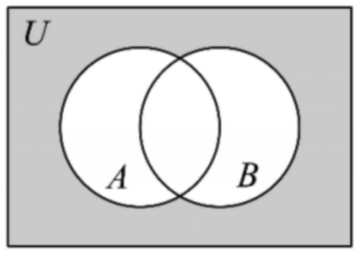
\includegraphics[width=0.20\textwidth]{figures/gao84_q9_venn.png}
\end{center}

\ifanswer
\solbegin
\step{$U=\{1,2,3,4,5,6,7,8,9,10\}$，$A=\{1,2\}$，$B=\{2,4\}$.}
\step{图中阴影部分表示的集合为 $\overline{A\cup B}=\{3,5,6,7,8,9,10\}$，共 $7$ 个元素，}
\step{其非空真子集的个数为 $2^7-2=126$.}
\solend
\fi

\item 若不等式 $ax^2-5x+c<0$ 的解集是 $(2,3)$，则不等式 $cx^2+5x+a\geqslant0$ 的解集是\blankline[4.4em].

\ifanswer
\solbegin
\step{若不等式 $ax^2-5x+c<0$ 的解集是 $(2,3)$，则 $a>0$ 且 $\begin{cases}\dfrac5a=5\\[2pt] \dfrac ca=6\end{cases}$，}
\step{则 $a=1$，$c=6$，}
\step{则不等式 $cx^2+5x+a\geqslant0$ 可化为 $6x^2+5x+1\geqslant0$，则 $x\leqslant-\dfrac12$ 或 $x\geqslant-\dfrac13$，}
\step{则不等式的解集为 $\left(-\infty,-\dfrac12\right]\cup\left[-\dfrac13,+\infty\right)$.}
\solend
\fi

\item 若关于 $x$ 的方程 $mx^2+2x+2=0$ 至少有一个负实根，则实数 $m$ 的取值范围是\blankline[4.4em].

\ifanswer
\solbegin
\step{①当 $m=0$ 时，方程为 $2x+2=0$，有一个负根，满足题意，}
\step{②当 $m\neq0$ 时，关于 $x$ 的方程 $mx^2+2x+2=0$ 至少有一个负根，}
\step{设根为 $x_1$、$x_2$，}
\step{当 $\Delta=4-8m=0$ 时，即 $m=\dfrac12$ 时，方程为 $\dfrac12x^2+2x+1=0$，}
\step{解得 $x=-2$，满足题意，}
\step{当 $\Delta=4-8m>0$，即 $m<\dfrac12$ 时，且 $m\neq0$ 时，}
\step{若有一个负根，则 $x_1x_2=\dfrac2m<0$，解得 $m<0$，}
\step{若有两个负根，则 $\begin{cases}x_1+x_2=-\dfrac2m<0\\[2pt] x_1x_2=\dfrac2m>0\end{cases}$，解得 $0<m<\dfrac12$，}
\step{综上所述，则实数 $m$ 的取值范围是 $\left(-\infty,\dfrac12\right]$.}
\solend
\fi

\item 设集合 $S$、$T$ 都至少含有两个元素，且 $S$、$T$ 同时满足：条件 1：对任意 $x$、$y\in S$，若
$x\neq y$，则 $x+y\in T$；条件 2：对任意 $x$、$y\in T$，若 $x\neq y$，则 $x-y\in S$. 给出下列说法：

①若 $S$ 只有 $2$ 个元素，则这 $2$ 个元素互为相反数；

②若 $S$ 只有 $2$ 个元素，则 $S\cup T$ 必有 $3$ 个元素；

③若 $S$ 只有 $2$ 个元素，则 $S\cup T$ 可能有 $4$ 个元素；

④存在含有 $3$ 个元素的集合 $S$，满足 $S\cup T$ 有 $4$ 个元素.

其中所有正确说法的序号是\blankline[4.4em].

\ifanswer
\solbegin
\step{对于①：由条件 2 得 $x-y\in S$，$y-x\in S$，且 $x-y\neq y-x$，}
\step{所以若 $S$ 只有 $2$ 个元素，则这 $2$ 个元素互为相反数，故①正确；}
\step{对于④：若 $S$ 有 $3$ 个元素，不妨设 $S=\{a,b,c\}$，其中 $a<b<c$，}
\step{则 $\{a+b,b+c,c+a\}\subseteq T$，所以 $c-a$、$c-b$、$b-a$、$a-c$、$b-c$、$a-b\in S$，}
\step{而 $c-a$ 与 $c-b$ 为两个互不相等的正数，$a-c$ 与 $a-b$ 为两个互不相等的负数，}
\step{故集合 $S$ 中至少有 $4$ 个元素，与 $S=\{a,b,c\}$ 有 $3$ 个元素矛盾，故④错误.}
\step{对于②③：若 $S$ 有 $2$ 个元素，由①得集合 $S$ 中的 $2$ 个元素必为相反数，}
\step{故可设 $S=\{a,-a\}(a\neq0)$. 由条件 1 得 $0\in T$，}
\step{由于集合 $T$ 中至少有 $2$ 个元素，故至少还有另外一个元素 $m\in T$.}
\step{当集合 $T$ 只有 $2$ 个元素时即 $T=\{0,m\}$，由条件 1 得 $-m\in S$，则 $m=\pm a$，}
\step{$T=\{0,a\}$ 或 $T=\{0,-a\}$，故 $S\cup T=\{0,a,-a\}$.}
\step{当集合 $T$ 有多于 $2$ 个元素时，不妨设 $T=\{0,m,n\}$，}
\step{则 $m$、$n$、$-m$、$-n$、$m-n$、$n-m\in S$，由于 $m$、$n\neq0$，}
\step{所以 $m\neq m-n$，$n\neq n-m$，又 $m\neq n$，}
\step{故集合 $S$ 至少有 $3$ 个元素，与 $S$ 中只有两个元素矛盾.}
\step{综上，$S\cup T=\{0,a,-a\}$，故②正确，③错误.}
\step{故正确的是①②.}
\solend
\fi

\end{enumerate}

\bigsec{二、选择题}

\begin{enumerate}
\setcounter{enumi}{12}

\item 用反证法证明命题：“若 $x+y>2$，则 $x>1$ 或 $y>1$”时，应假设\mbox{（\quad）}

\keepwithprev
A. $x\leqslant1$ 或 $y\leqslant1$\qquad B. 若 $x>1$ 或 $y>1$

C. $x\leqslant1$ 且 $y\leqslant1$\qquad D. 若 $x>1$ 且 $y>1$

\ifanswer
\ans{$C$}
\fi

\item 下列命题中，为真命题的是\mbox{（\quad）}

\keepwithprev
A. 若 $a>b$，则 $a^2>b^2$\qquad B. 若 $a>b$，$c>d$，则 $ac>bd$

C. 若 $a>b$，则 $\dfrac1a<\dfrac1b$\qquad D. 若 $ac^2>bc^2$，则 $a>b$

\ifanswer
\solbegin
\step{对于 $A$，当 $a=-1$，$b=-2$ 时，$a^2<b^2$，故 $A$ 错误；}
\step{对于 $B$，当 $a=-1$，$b=-2$，$c=-1$，$d=-2$ 时，$ac<bd$，故 $B$ 错误；}
\step{对于 $C$，当 $a=1$，$b=-2$ 时，$\dfrac1a>\dfrac1b$，故 $C$ 错误；}
\step{对于 $D$，因为 $ac^2-bc^2=(a-b)c^2>0$，所以 $a-b>0$，$c^2>0$，则 $a>b$，}
\step{故 $D$ 正确.}
\step{故选 $D$.}
\solend
\fi

\item 现有一级小麦 $m\,\mathrm{kg}$，二级小麦 $n\,\mathrm{kg}$，某粮食收购站有两种收购方案. 方案一：分两个
等级收购小麦，一级小麦 $a$ 元$/\mathrm{kg}$，二级小麦 $b$ 元$/\mathrm{kg}\,(b<a)$；方案二：以方案一两种价
格的平均数收购. 收购方式更加优惠的是\mbox{（\quad）}

\keepwithprev
A. 方案一\qquad B. 方案二\qquad C. 同样优惠\qquad D. 以上均有可能

\ifanswer
\solbegin
\step{方案一收购的平均价格为 $\dfrac{ma+nb}{m+n}$，方案二收购的平均价格为 $\dfrac{a+b}2$；}
\step{所以 $\dfrac{ma+nb}{m+n}-\dfrac{a+b}2=\dfrac{(a-b)(m-n)}{2(m+n)}$ ①，}
\step{$a-b>0$，$m-n$ 的正负性不确定，故①式的正负性不确定，故选 $D$.}
\solend
\fi

\item 用 $C(A)$ 表示非空集合 $A$ 中的元素个数. 对于集合 $A$、$B$，定义

$A*B=\begin{cases}C(A)-C(B),&C(A)\geqslant C(B)\\ C(B)-C(A),&C(A)<C(B)\end{cases}$，若 $A=\{0,1\}$，

$B=\{x\mid(x^2-ax)(x^2+ax+2)=0\}$，设实数 $a$ 的所有可能取值组成的集合是 $S$，则下列选
项不正确的是\mbox{（\quad）}

\keepwithprev
A. $C(B)$ 的可能值为 $1$，$2$，$3$，$4$

B. 若 $A*B=2$，则 $a$ 的取值范围为 $(-\infty,-2\sqrt2)\cup(2\sqrt2,+\infty)$

C. 若 $A*B=1$，则 $C(S)=3$

D. 若 $A*B=0$，则 $a$ 的取值范围为 $(-2\sqrt2,2\sqrt2)$

\ifanswer
\solbegin
\step{对于集合 $B$，当 $a=0$ 时，方程 $x^2(x^2+2)=0$ 的解为 $x=0$，$C(B)=1$，}
\step{当 $a\neq0$ 时，$x^2-ax=0$ 或 $x^2+ax+2=0$，}
\step{其中 $x^2-ax=0$ 的解为 $x_1=0$，$x_2=a$，}
\step{若 $\Delta=a^2-8>0$，即 $a>2\sqrt2$ 或 $a<-2\sqrt2$，}
\step{方程 $x^2+ax+2=0$ 有两个不相等的实数根，此时 $C(B)=4$；}
\step{若 $\Delta=a^2-8=0$，即 $a=2\sqrt2$ 或 $-2\sqrt2$，}
\step{方程 $x^2+ax+2=0$ 有两个相等的实数根，此时 $C(B)=3$；}
\step{若 $\Delta=a^2-8<0$，即 $-2\sqrt2<a<0$ 或 $0<a<2\sqrt2$，}
\step{方程 $x^2+ax+2=0$ 无实数根，此时 $C(B)=2$；}
\step{所以 $C(B)$ 的可能值为 $1$，$2$，$3$，$4$，故 $A$ 正确；}
\step{若 $A*B=2$，且 $C(A)=2$，则 $C(B)=4$，}
\step{则 $a$ 的取值范围 $(-\infty,-2\sqrt2)\cup(2\sqrt2,+\infty)$，故 $B$ 正确；}
\step{若 $A*B=1$，且 $C(A)=2$，则 $C(B)=1$ 或 $3$，}
\step{当 $C(B)=1$ 时，$a=0$，}
\step{当 $C(B)=3$ 时，$a=2\sqrt2$ 或 $-2\sqrt2$，此时集合 $S=\{0,-2\sqrt2,2\sqrt2\}$，}
\step{则 $C(S)=3$，故 $C$ 正确；}
\step{若 $A*B=0$，且 $C(A)=2$，则 $C(B)=2$，}
\step{由此可得 $a$ 的取值范围为 $(-2\sqrt2,0)\cup(0,2\sqrt2)$，故 $D$ 不正确；}
\step{故选 $D$.}
\solend
\fi

\end{enumerate}

\bigsec{三、解答题}

\begin{enumerate}
\setcounter{enumi}{16}

\item 已知集合 $A=\{x\mid-3<x\leqslant4\}$，集合 $B=\{x\mid k+1\leqslant x\leqslant2k-1\}$.

（1）当 $k=3$ 时，求 $A\cup B$、$\overline A\cap B$；

（2）若 $B\subseteq A$，求 $k$ 的取值范围.

\ansspace*[10]

\ifanswer
\solbegin
\stepm{（1）}{当 $k=3$ 时，$B=\{x\mid4\leqslant x\leqslant5\}$，又 $A=\{x\mid-3<x\leqslant4\}$，}
\step{所以 $\overline A=\{x\mid x\leqslant-3$ 或 $x>4\}$，}
\step{所以 $A\cup B=\{x\mid-3<x\leqslant5\}$，$\overline A\cap B=\{x\mid4<x\leqslant5\}$.}
\stepm{（2）}{①当 $B=\varnothing$，即 $k+1>2k-1$ 时，$k<2$，满足 $B\subseteq A$.}
\step{②当 $B\neq\varnothing$ 时，由 $B\subseteq A$ 得 $\begin{cases}k+1\leqslant2k-1\\ k+1>-3\\ 2k-1\leqslant4\end{cases}$，解得 $2\leqslant k\leqslant\dfrac52$，}
\step{综合①②得 $k$ 的取值范围 $\left\{k\mid k\leqslant\dfrac52\right\}$.}
\solend
\fi

\item 设集合 $A=\{x\mid x^2-3x+2=0\}$，$B=\{x\mid x^2+2(a+1)x+a^2-5=0\}$.

（1）若 $A\cap B=\{2\}$，求实数 $a$ 的值；

（2）若集合 $B$ 中有两个元素 $x_1,x_2$，求 $\lvert x_1-x_2\rvert$（用 $a$ 表示）.

\ansspace*[10]

\ifanswer
\solbegin
\stepm{（1）}{由题意得 $A=\{x\mid x^2-3x+2=0\}=\{1,2\}$，因为 $A\cap B=\{2\}$，所以 $2\in B$，}
\step{所以 $2^2+4(a+1)+a^2-5=0$ 即 $4+4a+4+a^2-5=0$，}
\step{化简得 $a^2+4a+3=0$，即 $(a+3)(a+1)=0$，解得 $a=-3$ 或 $a=-1$，}
\step{检验：当 $a=-3$ 时，$B=\{x\mid x^2-4x+4=0\}=\{2\}$，满足 $A\cap B=\{2\}$，}
\step{当 $a=-1$ 时，$B=\{x\mid x^2-4=0\}=\{-2,2\}$，满足 $A\cap B=\{2\}$，}
\step{所以 $a=-3$ 或 $a=-1$.}
\stepm{（2）}{因为 $B$ 中有两个元素 $x_1,x_2$，所以 $x^2+2(a+1)x+(a^2-5)=0$ 有两个根，}
\step{所以 $\Delta=4(a+1)^2-4(a^2-5)=8a+24>0$，}
\step{且 $x_1+x_2=-2(a+1)$，$x_1x_2=a^2-5$，}
\step{所以 $\lvert x_1-x_2\rvert=\sqrt{(x_1+x_2)^2-4x_1x_2}=\sqrt{4(a+1)^2-4(a^2-5)}=\sqrt{8a+24}$.}
\solend
\fi

\item 已知关于 $x$ 的不等式 $\dfrac{ax-2}{1+x}>0$.

（1）若 $x=-a$ 时，不等式成立，求实数 $a$ 的取值范围；

（2）若 $a$ 为实数，解关于 $x$ 的不等式：$\dfrac{ax-2}{1+x}>0$.

\ansspace*[12]

\ifanswer
\solbegin
\stepm{（1）}{因为 $x=-a$ 时，不等式成立，}
\step{所以 $\dfrac{-a^2-2}{1-a}>0\Rightarrow\dfrac{a^2+2}{a-1}>0\Rightarrow a-1>0\Rightarrow a>1$，}
\step{所以实数 $a$ 的取值范围为 $(1,+\infty)$.}
\stepm{（2）}{$\dfrac{ax-2}{1+x}>0\Rightarrow(ax-2)(x+1)>0$，}
\step{当 $a=0$ 时，$-2(x+1)>0$，解得 $x<-1$.}
\step{当 $a>0$ 时，$(ax-2)(x+1)>0$，解得 $x>\dfrac2a$ 或 $x<-1$.}
\step{当 $a<0$ 时，不等式 $(ax-2)(x+1)>0$ 可化为 $\left(x-\dfrac2a\right)(x+1)<0$，}
\step{当 $\dfrac2a>-1$，即 $a<-2$ 时，解得 $-1<x<\dfrac2a$；}
\step{当 $\dfrac2a<-1$，即 $-2<a<0$ 时，解得 $\dfrac2a<x<-1$；}
\step{当 $\dfrac2a=-1$，即 $a=-2$ 时，解集为 $\varnothing$.}
\step{综上，当 $a<-2$ 时，不等式的解集为 $\left(-1,\dfrac2a\right)$；}
\step{当 $a=-2$ 时，不等式的解集为 $\varnothing$；}
\step{当 $-2<a<0$ 时，不等式的解集为 $\left(\dfrac2a,-1\right)$；}
\step{当 $a=0$ 时，不等式的解集为 $(-\infty,-1)$；}
\step{当 $a>0$ 时，不等式的解集为 $(-\infty,-1)\cup\left(\dfrac2a,+\infty\right)$.}
\solend
\fi

\item 已知关于 $x$ 的不等式 $(k^2-2k-3)x^2+(k+1)x+1>0\,(k\in\R)$ 的解集为 $M$；

（1）若存在实数 $a$，使得 $M=(-\infty,a)\cup(a,+\infty)$，求 $k$ 的值；

（2）若 $M=\R$，求 $k$ 的取值范围；

（3）是否存在实数 $k$，满足：“对于任意 $n\in\N$，$n>0$，都有 $n\in M$；对于任意
$m\in\Z$，$m<0$，都有 $m\notin M$”，若存在，求出 $k$ 的值，若不存在，说明理由.

\ansspace*[13]

\ifanswer
\solbegin
\stepm{（1）}{记 $f(x)=(k^2-2k-3)x^2+(k+1)x+1$.}
\step{$M=(-\infty,a)\cup(a,+\infty)$ 表示 $f(x)>0$ 对一切 $x\neq a$ 成立，且 $f(a)=0$，}
\step{故需二次项系数大于 $0$ 且 $\Delta=0$.}
\step{由 $\Delta=(k+1)^2-4(k^2-2k-3)=-3k^2+10k+13=0$ 得 $k=\dfrac{13}3$ 或 $k=-1$.}
\step{当 $k=\dfrac{13}3$ 时，二次项系数 $\dfrac{64}9>0$，$f(x)=\dfrac{64}9\left(x+\dfrac38\right)^2$，符合；}
\step{当 $k=-1$ 时二次项系数为 $0$，$f(x)=1>0$，$M=\R$，不符合. 故 $k=\dfrac{13}3$.}
\stepm{（2）}{$M=\R$ 即 $f(x)>0$ 对一切 $x\in\R$ 恒成立.}
\step{①当 $k^2-2k-3>0$（即 $k<-1$ 或 $k>3$）时，需 $\Delta<0$，}
\step{即 $-3k^2+10k+13<0$，得 $k<-1$ 或 $k>\dfrac{13}3$，故 $k<-1$ 或 $k>\dfrac{13}3$；}
\step{②当 $k^2-2k-3=0$ 时，$k=3$ 得 $f(x)=4x+1$ 不恒正，不符合题意，}
\step{舍去，}
\step{当 $k=-1$ 得 $f(x)=1>0$ 恒成立，符合题意；}
\step{③当 $k^2-2k-3<0$ 时，抛物线开口向下，不能恒正.}
\step{综上，$k\leqslant-1$ 或 $k>\dfrac{13}3$.}
\stepm{（3）}{存在，$k=3$，理由如下，}
\step{由题意得解集 $M=(t,+\infty)$，$t\in[-1,1)$；}
\step{当 $k^2-2k-3=0$ 时，解得 $k=3$ 或 $k=-1$，}
\step{$k=3$ 时，不等式的解集为 $\left(-\dfrac14,+\infty\right)$，满足条件；}
\step{$k=-1$ 时，$1>0$ 恒成立，不满足条件；}
\step{当 $k^2-2k-3>0$ 时，}
\step{此时对应的一元二次不等式的解集形式不是 $(t,+\infty)$ 的形式，不满足条件；}
\step{当 $k^2-2k-3<0$ 时，}
\step{此时对应的一元二次不等式的解集形式不是 $(t,+\infty)$ 的形式，不满足条件；}
\step{综上，满足条件 $k$ 的值为 $3$.}
\solend
\fi

\item 已知有限集 $A=\{a_1,a_2,\cdots,a_n\}\,(n\geqslant2,n\in\N)$，如果 $A$ 中元素 $a_i\,(i=1,2,3,\cdots,n)$ 满足
$a_1+a_2+a_3+\cdots+a_n=a_1\times a_2\times\cdots\times a_n$，就称 $A$ 为“和积平衡集”.

（1）判断集合 $\{-1+\sqrt3,-1-\sqrt3\}$ 是否为“和积平衡集”；

（2）若 $a_1$、$a_2$ 是两个不同的正数，且 $\{a_1,a_2\}$ 是“和积平衡集”，写出以 $a_1$、$a_2$ 为根的一
个一元二次方程（系数可用 $a_1$、$a_2$ 表示），并证明 $a_1$、$a_2$ 至少有一个大于 $2$；

（3）若 $a_i\in\Z$ 且 $a_i>0$，求所有符合条件的“和积平衡集”.

\ansspace*[14]

\ifanswer
\solbegin
\stepm{（1）}{对于集合 $\{-1+\sqrt3,-1-\sqrt3\}$，}
\step{因为 $(-1+\sqrt3)+(-1-\sqrt3)=-2$，$(-1+\sqrt3)\times(-1-\sqrt3)=-2$，}
\step{所以满足 $a_1+a_2=a_1\times a_2$，满足题意，}
\step{所以集合 $\{-1+\sqrt3,-1-\sqrt3\}$ 是和积平衡集.}
\stepm{（2）}{以 $a_1$、$a_2$ 为根的一个一元二次方程可为 $x^2-(a_1+a_2)x+a_1\cdot a_2=0$，}
\step{因为 $a_1$、$a_2$ 是两个不同的正数，且 $\{a_1,a_2\}$ 是和积平衡集，}
\step{所以 $a_1+a_2=a_1\cdot a_2$，}
\step{又 $a_1$ 和 $a_2$ 为 $x^2-(a_1+a_2)x+a_1\cdot a_2=0$ 的两个不同的正根，}
\step{所以 $\Delta=(a_1+a_2)^2-4a_1a_2=(a_1+a_2)^2-4(a_1+a_2)>0$，}
\step{又 $a_1+a_2>0$，则 $a_1+a_2>4$，}
\step{若 $a_1$、$a_2$ 都小于等于 $2$，则 $a_1+a_2\leqslant4$，矛盾，}
\step{所以 $a_1$、$a_2$ 至少有一个大于 $2$；}
\stepm{（3）}{设 $A$ 中的 $a_1<a_2<a_3<\cdots<a_n$，且 $a_i\in\N^*$，}
\step{由 $a_1+a_2+a_3+\cdots+a_n=a_1\times a_2\times\cdots\times a_n$，得 $n=2$ 时明显不满足，}
\step{所以 $n\geqslant3$，故 $a_1\times a_2\times\cdots\times a_n=a_1+a_2+a_3+\cdots+a_n\leqslant na_n$，}
\step{所以 $a_1\times a_2\times\cdots\times a_{n-1}\leqslant n$，}
\step{当 $n=3$ 时，$a_1\times a_2\leqslant3$，$a_i\in\N^*$，只能有 $a_1=1$，$a_2=2$，}
\step{由 $a_1+a_2+a_3=a_1\times a_2\times a_3$，得 $a_3=3$，此时的和积平衡集为 $\{1,2,3\}$，}
\step{当 $n\geqslant4$ 时，$a_1\times a_2\times\cdots\times a_{n-1}\geqslant(n-1)(n-2)\times\cdots\times2\times1\geqslant(n-1)(n-2)$，}
\step{又 $(n-1)(n-2)-n=n^2-4n+2=n(n-4)+2>0$，即 $(n-1)(n-2)>n$，}
\step{即 $a_1\times a_2\times\cdots\times a_{n-1}>n$，与 $a_1\times a_2\times\cdots\times a_{n-1}\leqslant n$ 矛盾，}
\step{所以 $n\geqslant4$ 不满足条件，}
\step{所以符合条件的和积平衡集有且只有 $n=3$，此时的和积平衡集为 $\{1,2,3\}$.}
\solend
\fi

\end{enumerate}

\end{document}
"
%
% 原始材料：微信公众号“魔都数学加油站”文章，连载“27学年高一84”；
% 原文标题“27学年高一84——2026-2027年上海市东昌中学高一上10月月考”；
% 原文链接：https://mp.weixin.qq.com/s/PErsjO3N5RsMuJC69IGbrw。
% 页面标注发布时间 2026-10-26 20:15（上海）。
% 正文为 12 张 PNG 页（`原图/高一84_东昌中学_10月月考/01..12.png`），
% 尺寸混排（第 1—8 页为 4762×6735，第 9—12 页为 2560×3620），均按页序读取。
%
% 篇幅与题号：原卷自第 3 题起编号（第 1、2 题不在原文内）。填空题 3—12（10 题）、
% 选择题 13—16（4 题）、解答题 17—21（5 题），共 19 题。
%
% 讲评版：19 题全部印【解析】，本稿不另提 \ans{}；选择题答案在解析末句“故选 D／C／D”。
% 第 13 题的答案“C”原卷直接印在题干括号内（“（\ C\ ）”），本稿按 高一37 第 13 题／
% 高一63 第 14 题成例括号留空、另提 \ans{$C$}（该题无【解析】段）。
%
% 副标题：原卷未印副标题。本稿按内容标作“集合与常用逻辑用语、不等式”。
%
% 与原卷的排版差异：
%   ① 原卷每题下直接印【解析】，本稿按全稿惯例将解析置于答案版；
%   ② 原卷未印副标题，本稿补出；填空横线统一排 \blankline[4.4em]；
%   ③ 原卷数集记号排斜体 $R$、$Z$、$N$，本稿按全稿惯例改用 $\R$、$\Z$、$\N$；
%   ④ 第 17—21 题的子问用行内“（1）（2）（3）”段，解析中的子问标号用 \stepm；
%   ⑤ 解答题按惯例加 \ansspace；选择题括号排 \mbox{（\quad）}；
%   ⑥ 第 9 题题干右侧有一幅韦恩图，裁自原图（第 2 页）后去粉色水印、转灰度，
%      三版都出（属题干）。
%
% 行数核对：逐题数 \step/\stepm 条数，合计 157 条（Q3：2；Q4：2；Q5：3；Q6：2；
% Q7：3；Q8：6；Q9：3；Q10：4；Q11：9；Q12：17；Q14：6；Q15：3；Q16：19；
% Q17：6；Q18：10；Q19：15；Q20：24；Q21：23）；第 13 题无解析，只提 \ans{}，
% 不计入 \step 账。原卷解析的换行按语意合并，未逐行强拆。
%
\documentclass[a4paper,11pt]{article}
\usepackage{common}

\begin{document}

\examtitlest[4]{2026--2027 年东昌中学高一上 10 月月考}{集合与常用逻辑用语、不等式}

\bigsec{一、填空题}

\begin{enumerate}
\setcounter{enumi}{2}

\item 若 $a\in\R$，则“$a=2$”是“$(a-1)(a-2)=0$”的\blankline[3.6em]条件（填“充分不必要”、“必要
不充分”、“充要”、“既不充分又不必要”的一个）.

\ifanswer
\solbegin
\step{$a=2\Rightarrow(a-1)(a-2)=0$，而 $(a-1)(a-2)=0$ 不能推出 $a=2$，}
\step{故“$a=2$”是“$(a-1)(a-2)=0$”的充分不必要条件.}
\solend
\fi

\item 已知集合 $M=\{(x,y)\mid y=x^2\}$，$N=\{(x,y)\mid y=1\}$，则 $M\cap N=\blankline[4.4em]$.

\ifanswer
\solbegin
\step{集合 $M=\{(x,y)\mid y=x^2\}$，$N=\{(x,y)\mid y=1\}$，}
\step{当 $y=1$ 时，$x=\pm1$，则 $M\cap N=\{(-1,1),(1,1)\}$.}
\solend
\fi

\item 已知集合 $A=\{x\mid x^2+ax+4=0\}$，若 $A$ 有且只有一个非空子集，则实数 $a=\blankline[4.4em]$.

\ifanswer
\solbegin
\step{因为集合 $A$ 有且只有一个非空子集，所以集合 $A$ 中只有一个元素，}
\step{所以一元二次方程 $x^2+ax+4=0$ 有两个相等的解，}
\step{所以 $\Delta=a^2-4\times4=0$，解得 $a=\pm4$.}
\solend
\fi

\item 已知 $A=(-\infty,a]$，$B=(-\infty,3)$，且 $x\in A$ 是 $x\in B$ 的充分不必要条件，则 $a$ 的取值范围
是\blankline[4.4em].

\ifanswer
\solbegin
\step{$A=(-\infty,a]$，$B=(-\infty,3)$，且 $x\in A$ 是 $x\in B$ 的充分不必要条件，}
\step{则 $A\subset B$，则 $a<3$，即 $a$ 的取值范围为 $(-\infty,3)$.}
\solend
\fi

\item 不等式 $\dfrac{3x-1}{x-2}\leqslant1$ 的解集为\blankline[4.4em].

\ifanswer
\solbegin
\step{由 $\dfrac{3x-1}{x-2}\leqslant1$，得 $\dfrac{3x-1}{x-2}-1=\dfrac{3x-1-(x-2)}{x-2}=\dfrac{2x+1}{x-2}\leqslant0$，}
\step{则 $\begin{cases}(2x+1)(x-2)\leqslant0\\ x-2\neq0\end{cases}$，解得 $-\dfrac12\leqslant x<2$，}
\step{则不等式 $\dfrac{3x-1}{x-2}\leqslant1$ 的解集为 $\left[-\dfrac12,2\right)$.}
\solend
\fi

\item 已知关于 $x$ 的一元二次方程 $x^2-2mx+(3m+1)=0$ 的两个实数根为 $x_1$、$x_2$，且
$x_1^2+x_2^2=16$，则实数 $m$ 的值为\blankline[4.4em].

\ifanswer
\solbegin
\step{由韦达定理，得 $x_1+x_2=2m$，$x_1x_2=3m+1$，}
\step{$x_1^2+x_2^2=(x_1+x_2)^2-2x_1x_2=4m^2-6m-2$，}
\step{由 $x_1^2+x_2^2=16$，得 $4m^2-6m-2=16$，即 $2m^2-3m-9=0$，}
\step{解得 $m=3$ 或 $m=-\dfrac32$，}
\step{检验判别式 $\Delta=4m^2-12m-4$，当 $m=3$ 时，$\Delta=-4<0$，舍去；}
\step{当 $m=-\dfrac32$ 时，$\Delta=23>0$，符合条件，故 $m=-\dfrac32$.}
\solend
\fi

\item 已知全集 $U=\{x\mid1\leqslant x\leqslant10,\,x\in\N\}$，集合 $A=\{x\mid x^2-3<4,\,x\in\N,\,x>0\}$，
$B=\{2,4\}$，则图中阴影部分表示的集合的非空真子集个数为\blankline[4.4em].

\needvspace{9\baselineskip}
\begin{center}
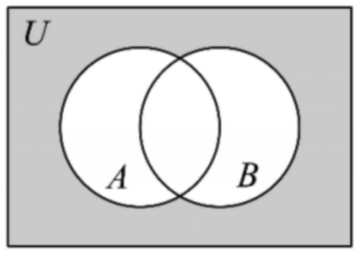
\includegraphics[width=0.20\textwidth]{figures/gao84_q9_venn.png}
\end{center}

\ifanswer
\solbegin
\step{$U=\{1,2,3,4,5,6,7,8,9,10\}$，$A=\{1,2\}$，$B=\{2,4\}$.}
\step{图中阴影部分表示的集合为 $\overline{A\cup B}=\{3,5,6,7,8,9,10\}$，共 $7$ 个元素，}
\step{其非空真子集的个数为 $2^7-2=126$.}
\solend
\fi

\item 若不等式 $ax^2-5x+c<0$ 的解集是 $(2,3)$，则不等式 $cx^2+5x+a\geqslant0$ 的解集是\blankline[4.4em].

\ifanswer
\solbegin
\step{若不等式 $ax^2-5x+c<0$ 的解集是 $(2,3)$，则 $a>0$ 且 $\begin{cases}\dfrac5a=5\\[2pt] \dfrac ca=6\end{cases}$，}
\step{则 $a=1$，$c=6$，}
\step{则不等式 $cx^2+5x+a\geqslant0$ 可化为 $6x^2+5x+1\geqslant0$，则 $x\leqslant-\dfrac12$ 或 $x\geqslant-\dfrac13$，}
\step{则不等式的解集为 $\left(-\infty,-\dfrac12\right]\cup\left[-\dfrac13,+\infty\right)$.}
\solend
\fi

\item 若关于 $x$ 的方程 $mx^2+2x+2=0$ 至少有一个负实根，则实数 $m$ 的取值范围是\blankline[4.4em].

\ifanswer
\solbegin
\step{①当 $m=0$ 时，方程为 $2x+2=0$，有一个负根，满足题意，}
\step{②当 $m\neq0$ 时，关于 $x$ 的方程 $mx^2+2x+2=0$ 至少有一个负根，}
\step{设根为 $x_1$、$x_2$，}
\step{当 $\Delta=4-8m=0$ 时，即 $m=\dfrac12$ 时，方程为 $\dfrac12x^2+2x+1=0$，}
\step{解得 $x=-2$，满足题意，}
\step{当 $\Delta=4-8m>0$，即 $m<\dfrac12$ 时，且 $m\neq0$ 时，}
\step{若有一个负根，则 $x_1x_2=\dfrac2m<0$，解得 $m<0$，}
\step{若有两个负根，则 $\begin{cases}x_1+x_2=-\dfrac2m<0\\[2pt] x_1x_2=\dfrac2m>0\end{cases}$，解得 $0<m<\dfrac12$，}
\step{综上所述，则实数 $m$ 的取值范围是 $\left(-\infty,\dfrac12\right]$.}
\solend
\fi

\item 设集合 $S$、$T$ 都至少含有两个元素，且 $S$、$T$ 同时满足：条件 1：对任意 $x$、$y\in S$，若
$x\neq y$，则 $x+y\in T$；条件 2：对任意 $x$、$y\in T$，若 $x\neq y$，则 $x-y\in S$. 给出下列说法：

①若 $S$ 只有 $2$ 个元素，则这 $2$ 个元素互为相反数；

②若 $S$ 只有 $2$ 个元素，则 $S\cup T$ 必有 $3$ 个元素；

③若 $S$ 只有 $2$ 个元素，则 $S\cup T$ 可能有 $4$ 个元素；

④存在含有 $3$ 个元素的集合 $S$，满足 $S\cup T$ 有 $4$ 个元素.

其中所有正确说法的序号是\blankline[4.4em].

\ifanswer
\solbegin
\step{对于①：由条件 2 得 $x-y\in S$，$y-x\in S$，且 $x-y\neq y-x$，}
\step{所以若 $S$ 只有 $2$ 个元素，则这 $2$ 个元素互为相反数，故①正确；}
\step{对于④：若 $S$ 有 $3$ 个元素，不妨设 $S=\{a,b,c\}$，其中 $a<b<c$，}
\step{则 $\{a+b,b+c,c+a\}\subseteq T$，所以 $c-a$、$c-b$、$b-a$、$a-c$、$b-c$、$a-b\in S$，}
\step{而 $c-a$ 与 $c-b$ 为两个互不相等的正数，$a-c$ 与 $a-b$ 为两个互不相等的负数，}
\step{故集合 $S$ 中至少有 $4$ 个元素，与 $S=\{a,b,c\}$ 有 $3$ 个元素矛盾，故④错误.}
\step{对于②③：若 $S$ 有 $2$ 个元素，由①得集合 $S$ 中的 $2$ 个元素必为相反数，}
\step{故可设 $S=\{a,-a\}(a\neq0)$. 由条件 1 得 $0\in T$，}
\step{由于集合 $T$ 中至少有 $2$ 个元素，故至少还有另外一个元素 $m\in T$.}
\step{当集合 $T$ 只有 $2$ 个元素时即 $T=\{0,m\}$，由条件 1 得 $-m\in S$，则 $m=\pm a$，}
\step{$T=\{0,a\}$ 或 $T=\{0,-a\}$，故 $S\cup T=\{0,a,-a\}$.}
\step{当集合 $T$ 有多于 $2$ 个元素时，不妨设 $T=\{0,m,n\}$，}
\step{则 $m$、$n$、$-m$、$-n$、$m-n$、$n-m\in S$，由于 $m$、$n\neq0$，}
\step{所以 $m\neq m-n$，$n\neq n-m$，又 $m\neq n$，}
\step{故集合 $S$ 至少有 $3$ 个元素，与 $S$ 中只有两个元素矛盾.}
\step{综上，$S\cup T=\{0,a,-a\}$，故②正确，③错误.}
\step{故正确的是①②.}
\solend
\fi

\end{enumerate}

\bigsec{二、选择题}

\begin{enumerate}
\setcounter{enumi}{12}

\item 用反证法证明命题：“若 $x+y>2$，则 $x>1$ 或 $y>1$”时，应假设\mbox{（\quad）}

\keepwithprev
A. $x\leqslant1$ 或 $y\leqslant1$\qquad B. 若 $x>1$ 或 $y>1$

C. $x\leqslant1$ 且 $y\leqslant1$\qquad D. 若 $x>1$ 且 $y>1$

\ifanswer
\ans{$C$}
\fi

\item 下列命题中，为真命题的是\mbox{（\quad）}

\keepwithprev
A. 若 $a>b$，则 $a^2>b^2$\qquad B. 若 $a>b$，$c>d$，则 $ac>bd$

C. 若 $a>b$，则 $\dfrac1a<\dfrac1b$\qquad D. 若 $ac^2>bc^2$，则 $a>b$

\ifanswer
\solbegin
\step{对于 $A$，当 $a=-1$，$b=-2$ 时，$a^2<b^2$，故 $A$ 错误；}
\step{对于 $B$，当 $a=-1$，$b=-2$，$c=-1$，$d=-2$ 时，$ac<bd$，故 $B$ 错误；}
\step{对于 $C$，当 $a=1$，$b=-2$ 时，$\dfrac1a>\dfrac1b$，故 $C$ 错误；}
\step{对于 $D$，因为 $ac^2-bc^2=(a-b)c^2>0$，所以 $a-b>0$，$c^2>0$，则 $a>b$，}
\step{故 $D$ 正确.}
\step{故选 $D$.}
\solend
\fi

\item 现有一级小麦 $m\,\mathrm{kg}$，二级小麦 $n\,\mathrm{kg}$，某粮食收购站有两种收购方案. 方案一：分两个
等级收购小麦，一级小麦 $a$ 元$/\mathrm{kg}$，二级小麦 $b$ 元$/\mathrm{kg}\,(b<a)$；方案二：以方案一两种价
格的平均数收购. 收购方式更加优惠的是\mbox{（\quad）}

\keepwithprev
A. 方案一\qquad B. 方案二\qquad C. 同样优惠\qquad D. 以上均有可能

\ifanswer
\solbegin
\step{方案一收购的平均价格为 $\dfrac{ma+nb}{m+n}$，方案二收购的平均价格为 $\dfrac{a+b}2$；}
\step{所以 $\dfrac{ma+nb}{m+n}-\dfrac{a+b}2=\dfrac{(a-b)(m-n)}{2(m+n)}$ ①，}
\step{$a-b>0$，$m-n$ 的正负性不确定，故①式的正负性不确定，故选 $D$.}
\solend
\fi

\item 用 $C(A)$ 表示非空集合 $A$ 中的元素个数. 对于集合 $A$、$B$，定义

$A*B=\begin{cases}C(A)-C(B),&C(A)\geqslant C(B)\\ C(B)-C(A),&C(A)<C(B)\end{cases}$，若 $A=\{0,1\}$，

$B=\{x\mid(x^2-ax)(x^2+ax+2)=0\}$，设实数 $a$ 的所有可能取值组成的集合是 $S$，则下列选
项不正确的是\mbox{（\quad）}

\keepwithprev
A. $C(B)$ 的可能值为 $1$，$2$，$3$，$4$

B. 若 $A*B=2$，则 $a$ 的取值范围为 $(-\infty,-2\sqrt2)\cup(2\sqrt2,+\infty)$

C. 若 $A*B=1$，则 $C(S)=3$

D. 若 $A*B=0$，则 $a$ 的取值范围为 $(-2\sqrt2,2\sqrt2)$

\ifanswer
\solbegin
\step{对于集合 $B$，当 $a=0$ 时，方程 $x^2(x^2+2)=0$ 的解为 $x=0$，$C(B)=1$，}
\step{当 $a\neq0$ 时，$x^2-ax=0$ 或 $x^2+ax+2=0$，}
\step{其中 $x^2-ax=0$ 的解为 $x_1=0$，$x_2=a$，}
\step{若 $\Delta=a^2-8>0$，即 $a>2\sqrt2$ 或 $a<-2\sqrt2$，}
\step{方程 $x^2+ax+2=0$ 有两个不相等的实数根，此时 $C(B)=4$；}
\step{若 $\Delta=a^2-8=0$，即 $a=2\sqrt2$ 或 $-2\sqrt2$，}
\step{方程 $x^2+ax+2=0$ 有两个相等的实数根，此时 $C(B)=3$；}
\step{若 $\Delta=a^2-8<0$，即 $-2\sqrt2<a<0$ 或 $0<a<2\sqrt2$，}
\step{方程 $x^2+ax+2=0$ 无实数根，此时 $C(B)=2$；}
\step{所以 $C(B)$ 的可能值为 $1$，$2$，$3$，$4$，故 $A$ 正确；}
\step{若 $A*B=2$，且 $C(A)=2$，则 $C(B)=4$，}
\step{则 $a$ 的取值范围 $(-\infty,-2\sqrt2)\cup(2\sqrt2,+\infty)$，故 $B$ 正确；}
\step{若 $A*B=1$，且 $C(A)=2$，则 $C(B)=1$ 或 $3$，}
\step{当 $C(B)=1$ 时，$a=0$，}
\step{当 $C(B)=3$ 时，$a=2\sqrt2$ 或 $-2\sqrt2$，此时集合 $S=\{0,-2\sqrt2,2\sqrt2\}$，}
\step{则 $C(S)=3$，故 $C$ 正确；}
\step{若 $A*B=0$，且 $C(A)=2$，则 $C(B)=2$，}
\step{由此可得 $a$ 的取值范围为 $(-2\sqrt2,0)\cup(0,2\sqrt2)$，故 $D$ 不正确；}
\step{故选 $D$.}
\solend
\fi

\end{enumerate}

\bigsec{三、解答题}

\begin{enumerate}
\setcounter{enumi}{16}

\item 已知集合 $A=\{x\mid-3<x\leqslant4\}$，集合 $B=\{x\mid k+1\leqslant x\leqslant2k-1\}$.

（1）当 $k=3$ 时，求 $A\cup B$、$\overline A\cap B$；

（2）若 $B\subseteq A$，求 $k$ 的取值范围.

\ansspace*[10]

\ifanswer
\solbegin
\stepm{（1）}{当 $k=3$ 时，$B=\{x\mid4\leqslant x\leqslant5\}$，又 $A=\{x\mid-3<x\leqslant4\}$，}
\step{所以 $\overline A=\{x\mid x\leqslant-3$ 或 $x>4\}$，}
\step{所以 $A\cup B=\{x\mid-3<x\leqslant5\}$，$\overline A\cap B=\{x\mid4<x\leqslant5\}$.}
\stepm{（2）}{①当 $B=\varnothing$，即 $k+1>2k-1$ 时，$k<2$，满足 $B\subseteq A$.}
\step{②当 $B\neq\varnothing$ 时，由 $B\subseteq A$ 得 $\begin{cases}k+1\leqslant2k-1\\ k+1>-3\\ 2k-1\leqslant4\end{cases}$，解得 $2\leqslant k\leqslant\dfrac52$，}
\step{综合①②得 $k$ 的取值范围 $\left\{k\mid k\leqslant\dfrac52\right\}$.}
\solend
\fi

\item 设集合 $A=\{x\mid x^2-3x+2=0\}$，$B=\{x\mid x^2+2(a+1)x+a^2-5=0\}$.

（1）若 $A\cap B=\{2\}$，求实数 $a$ 的值；

（2）若集合 $B$ 中有两个元素 $x_1,x_2$，求 $\lvert x_1-x_2\rvert$（用 $a$ 表示）.

\ansspace*[10]

\ifanswer
\solbegin
\stepm{（1）}{由题意得 $A=\{x\mid x^2-3x+2=0\}=\{1,2\}$，因为 $A\cap B=\{2\}$，所以 $2\in B$，}
\step{所以 $2^2+4(a+1)+a^2-5=0$ 即 $4+4a+4+a^2-5=0$，}
\step{化简得 $a^2+4a+3=0$，即 $(a+3)(a+1)=0$，解得 $a=-3$ 或 $a=-1$，}
\step{检验：当 $a=-3$ 时，$B=\{x\mid x^2-4x+4=0\}=\{2\}$，满足 $A\cap B=\{2\}$，}
\step{当 $a=-1$ 时，$B=\{x\mid x^2-4=0\}=\{-2,2\}$，满足 $A\cap B=\{2\}$，}
\step{所以 $a=-3$ 或 $a=-1$.}
\stepm{（2）}{因为 $B$ 中有两个元素 $x_1,x_2$，所以 $x^2+2(a+1)x+(a^2-5)=0$ 有两个根，}
\step{所以 $\Delta=4(a+1)^2-4(a^2-5)=8a+24>0$，}
\step{且 $x_1+x_2=-2(a+1)$，$x_1x_2=a^2-5$，}
\step{所以 $\lvert x_1-x_2\rvert=\sqrt{(x_1+x_2)^2-4x_1x_2}=\sqrt{4(a+1)^2-4(a^2-5)}=\sqrt{8a+24}$.}
\solend
\fi

\item 已知关于 $x$ 的不等式 $\dfrac{ax-2}{1+x}>0$.

（1）若 $x=-a$ 时，不等式成立，求实数 $a$ 的取值范围；

（2）若 $a$ 为实数，解关于 $x$ 的不等式：$\dfrac{ax-2}{1+x}>0$.

\ansspace*[12]

\ifanswer
\solbegin
\stepm{（1）}{因为 $x=-a$ 时，不等式成立，}
\step{所以 $\dfrac{-a^2-2}{1-a}>0\Rightarrow\dfrac{a^2+2}{a-1}>0\Rightarrow a-1>0\Rightarrow a>1$，}
\step{所以实数 $a$ 的取值范围为 $(1,+\infty)$.}
\stepm{（2）}{$\dfrac{ax-2}{1+x}>0\Rightarrow(ax-2)(x+1)>0$，}
\step{当 $a=0$ 时，$-2(x+1)>0$，解得 $x<-1$.}
\step{当 $a>0$ 时，$(ax-2)(x+1)>0$，解得 $x>\dfrac2a$ 或 $x<-1$.}
\step{当 $a<0$ 时，不等式 $(ax-2)(x+1)>0$ 可化为 $\left(x-\dfrac2a\right)(x+1)<0$，}
\step{当 $\dfrac2a>-1$，即 $a<-2$ 时，解得 $-1<x<\dfrac2a$；}
\step{当 $\dfrac2a<-1$，即 $-2<a<0$ 时，解得 $\dfrac2a<x<-1$；}
\step{当 $\dfrac2a=-1$，即 $a=-2$ 时，解集为 $\varnothing$.}
\step{综上，当 $a<-2$ 时，不等式的解集为 $\left(-1,\dfrac2a\right)$；}
\step{当 $a=-2$ 时，不等式的解集为 $\varnothing$；}
\step{当 $-2<a<0$ 时，不等式的解集为 $\left(\dfrac2a,-1\right)$；}
\step{当 $a=0$ 时，不等式的解集为 $(-\infty,-1)$；}
\step{当 $a>0$ 时，不等式的解集为 $(-\infty,-1)\cup\left(\dfrac2a,+\infty\right)$.}
\solend
\fi

\item 已知关于 $x$ 的不等式 $(k^2-2k-3)x^2+(k+1)x+1>0\,(k\in\R)$ 的解集为 $M$；

（1）若存在实数 $a$，使得 $M=(-\infty,a)\cup(a,+\infty)$，求 $k$ 的值；

（2）若 $M=\R$，求 $k$ 的取值范围；

（3）是否存在实数 $k$，满足：“对于任意 $n\in\N$，$n>0$，都有 $n\in M$；对于任意
$m\in\Z$，$m<0$，都有 $m\notin M$”，若存在，求出 $k$ 的值，若不存在，说明理由.

\ansspace*[13]

\ifanswer
\solbegin
\stepm{（1）}{记 $f(x)=(k^2-2k-3)x^2+(k+1)x+1$.}
\step{$M=(-\infty,a)\cup(a,+\infty)$ 表示 $f(x)>0$ 对一切 $x\neq a$ 成立，且 $f(a)=0$，}
\step{故需二次项系数大于 $0$ 且 $\Delta=0$.}
\step{由 $\Delta=(k+1)^2-4(k^2-2k-3)=-3k^2+10k+13=0$ 得 $k=\dfrac{13}3$ 或 $k=-1$.}
\step{当 $k=\dfrac{13}3$ 时，二次项系数 $\dfrac{64}9>0$，$f(x)=\dfrac{64}9\left(x+\dfrac38\right)^2$，符合；}
\step{当 $k=-1$ 时二次项系数为 $0$，$f(x)=1>0$，$M=\R$，不符合. 故 $k=\dfrac{13}3$.}
\stepm{（2）}{$M=\R$ 即 $f(x)>0$ 对一切 $x\in\R$ 恒成立.}
\step{①当 $k^2-2k-3>0$（即 $k<-1$ 或 $k>3$）时，需 $\Delta<0$，}
\step{即 $-3k^2+10k+13<0$，得 $k<-1$ 或 $k>\dfrac{13}3$，故 $k<-1$ 或 $k>\dfrac{13}3$；}
\step{②当 $k^2-2k-3=0$ 时，$k=3$ 得 $f(x)=4x+1$ 不恒正，不符合题意，}
\step{舍去，}
\step{当 $k=-1$ 得 $f(x)=1>0$ 恒成立，符合题意；}
\step{③当 $k^2-2k-3<0$ 时，抛物线开口向下，不能恒正.}
\step{综上，$k\leqslant-1$ 或 $k>\dfrac{13}3$.}
\stepm{（3）}{存在，$k=3$，理由如下，}
\step{由题意得解集 $M=(t,+\infty)$，$t\in[-1,1)$；}
\step{当 $k^2-2k-3=0$ 时，解得 $k=3$ 或 $k=-1$，}
\step{$k=3$ 时，不等式的解集为 $\left(-\dfrac14,+\infty\right)$，满足条件；}
\step{$k=-1$ 时，$1>0$ 恒成立，不满足条件；}
\step{当 $k^2-2k-3>0$ 时，}
\step{此时对应的一元二次不等式的解集形式不是 $(t,+\infty)$ 的形式，不满足条件；}
\step{当 $k^2-2k-3<0$ 时，}
\step{此时对应的一元二次不等式的解集形式不是 $(t,+\infty)$ 的形式，不满足条件；}
\step{综上，满足条件 $k$ 的值为 $3$.}
\solend
\fi

\item 已知有限集 $A=\{a_1,a_2,\cdots,a_n\}\,(n\geqslant2,n\in\N)$，如果 $A$ 中元素 $a_i\,(i=1,2,3,\cdots,n)$ 满足
$a_1+a_2+a_3+\cdots+a_n=a_1\times a_2\times\cdots\times a_n$，就称 $A$ 为“和积平衡集”.

（1）判断集合 $\{-1+\sqrt3,-1-\sqrt3\}$ 是否为“和积平衡集”；

（2）若 $a_1$、$a_2$ 是两个不同的正数，且 $\{a_1,a_2\}$ 是“和积平衡集”，写出以 $a_1$、$a_2$ 为根的一
个一元二次方程（系数可用 $a_1$、$a_2$ 表示），并证明 $a_1$、$a_2$ 至少有一个大于 $2$；

（3）若 $a_i\in\Z$ 且 $a_i>0$，求所有符合条件的“和积平衡集”.

\ansspace*[14]

\ifanswer
\solbegin
\stepm{（1）}{对于集合 $\{-1+\sqrt3,-1-\sqrt3\}$，}
\step{因为 $(-1+\sqrt3)+(-1-\sqrt3)=-2$，$(-1+\sqrt3)\times(-1-\sqrt3)=-2$，}
\step{所以满足 $a_1+a_2=a_1\times a_2$，满足题意，}
\step{所以集合 $\{-1+\sqrt3,-1-\sqrt3\}$ 是和积平衡集.}
\stepm{（2）}{以 $a_1$、$a_2$ 为根的一个一元二次方程可为 $x^2-(a_1+a_2)x+a_1\cdot a_2=0$，}
\step{因为 $a_1$、$a_2$ 是两个不同的正数，且 $\{a_1,a_2\}$ 是和积平衡集，}
\step{所以 $a_1+a_2=a_1\cdot a_2$，}
\step{又 $a_1$ 和 $a_2$ 为 $x^2-(a_1+a_2)x+a_1\cdot a_2=0$ 的两个不同的正根，}
\step{所以 $\Delta=(a_1+a_2)^2-4a_1a_2=(a_1+a_2)^2-4(a_1+a_2)>0$，}
\step{又 $a_1+a_2>0$，则 $a_1+a_2>4$，}
\step{若 $a_1$、$a_2$ 都小于等于 $2$，则 $a_1+a_2\leqslant4$，矛盾，}
\step{所以 $a_1$、$a_2$ 至少有一个大于 $2$；}
\stepm{（3）}{设 $A$ 中的 $a_1<a_2<a_3<\cdots<a_n$，且 $a_i\in\N^*$，}
\step{由 $a_1+a_2+a_3+\cdots+a_n=a_1\times a_2\times\cdots\times a_n$，得 $n=2$ 时明显不满足，}
\step{所以 $n\geqslant3$，故 $a_1\times a_2\times\cdots\times a_n=a_1+a_2+a_3+\cdots+a_n\leqslant na_n$，}
\step{所以 $a_1\times a_2\times\cdots\times a_{n-1}\leqslant n$，}
\step{当 $n=3$ 时，$a_1\times a_2\leqslant3$，$a_i\in\N^*$，只能有 $a_1=1$，$a_2=2$，}
\step{由 $a_1+a_2+a_3=a_1\times a_2\times a_3$，得 $a_3=3$，此时的和积平衡集为 $\{1,2,3\}$，}
\step{当 $n\geqslant4$ 时，$a_1\times a_2\times\cdots\times a_{n-1}\geqslant(n-1)(n-2)\times\cdots\times2\times1\geqslant(n-1)(n-2)$，}
\step{又 $(n-1)(n-2)-n=n^2-4n+2=n(n-4)+2>0$，即 $(n-1)(n-2)>n$，}
\step{即 $a_1\times a_2\times\cdots\times a_{n-1}>n$，与 $a_1\times a_2\times\cdots\times a_{n-1}\leqslant n$ 矛盾，}
\step{所以 $n\geqslant4$ 不满足条件，}
\step{所以符合条件的和积平衡集有且只有 $n=3$，此时的和积平衡集为 $\{1,2,3\}$.}
\solend
\fi

\end{enumerate}

\end{document}
"
%
% 原始材料：微信公众号“魔都数学加油站”文章，连载“27学年高一84”；
% 原文标题“27学年高一84——2026-2027年上海市东昌中学高一上10月月考”；
% 原文链接：https://mp.weixin.qq.com/s/PErsjO3N5RsMuJC69IGbrw。
% 页面标注发布时间 2026-10-26 20:15（上海）。
% 正文为 12 张 PNG 页（`原图/高一84_东昌中学_10月月考/01..12.png`），
% 尺寸混排（第 1—8 页为 4762×6735，第 9—12 页为 2560×3620），均按页序读取。
%
% 篇幅与题号：原卷自第 3 题起编号（第 1、2 题不在原文内）。填空题 3—12（10 题）、
% 选择题 13—16（4 题）、解答题 17—21（5 题），共 19 题。
%
% 讲评版：19 题全部印【解析】，本稿不另提 \ans{}；选择题答案在解析末句“故选 D／C／D”。
% 第 13 题的答案“C”原卷直接印在题干括号内（“（\ C\ ）”），本稿按 高一37 第 13 题／
% 高一63 第 14 题成例括号留空、另提 \ans{$C$}（该题无【解析】段）。
%
% 副标题：原卷未印副标题。本稿按内容标作“集合与常用逻辑用语、不等式”。
%
% 与原卷的排版差异：
%   ① 原卷每题下直接印【解析】，本稿按全稿惯例将解析置于答案版；
%   ② 原卷未印副标题，本稿补出；填空横线统一排 \blankline[4.4em]；
%   ③ 原卷数集记号排斜体 $R$、$Z$、$N$，本稿按全稿惯例改用 $\R$、$\Z$、$\N$；
%   ④ 第 17—21 题的子问用行内“（1）（2）（3）”段，解析中的子问标号用 \stepm；
%   ⑤ 解答题按惯例加 \ansspace；选择题括号排 \mbox{（\quad）}；
%   ⑥ 第 9 题题干右侧有一幅韦恩图，裁自原图（第 2 页）后去粉色水印、转灰度，
%      三版都出（属题干）。
%
% 行数核对：逐题数 \step/\stepm 条数，合计 157 条（Q3：2；Q4：2；Q5：3；Q6：2；
% Q7：3；Q8：6；Q9：3；Q10：4；Q11：9；Q12：17；Q14：6；Q15：3；Q16：19；
% Q17：6；Q18：10；Q19：15；Q20：24；Q21：23）；第 13 题无解析，只提 \ans{}，
% 不计入 \step 账。原卷解析的换行按语意合并，未逐行强拆。
%
\documentclass[a4paper,11pt]{article}
\usepackage{common}

\begin{document}

\examtitlest[4]{2026--2027 年东昌中学高一上 10 月月考}{集合与常用逻辑用语、不等式}

\bigsec{一、填空题}

\begin{enumerate}
\setcounter{enumi}{2}

\item 若 $a\in\R$，则“$a=2$”是“$(a-1)(a-2)=0$”的\blankline[3.6em]条件（填“充分不必要”、“必要
不充分”、“充要”、“既不充分又不必要”的一个）.

\ifanswer
\solbegin
\step{$a=2\Rightarrow(a-1)(a-2)=0$，而 $(a-1)(a-2)=0$ 不能推出 $a=2$，}
\step{故“$a=2$”是“$(a-1)(a-2)=0$”的充分不必要条件.}
\solend
\fi

\item 已知集合 $M=\{(x,y)\mid y=x^2\}$，$N=\{(x,y)\mid y=1\}$，则 $M\cap N=\blankline[4.4em]$.

\ifanswer
\solbegin
\step{集合 $M=\{(x,y)\mid y=x^2\}$，$N=\{(x,y)\mid y=1\}$，}
\step{当 $y=1$ 时，$x=\pm1$，则 $M\cap N=\{(-1,1),(1,1)\}$.}
\solend
\fi

\item 已知集合 $A=\{x\mid x^2+ax+4=0\}$，若 $A$ 有且只有一个非空子集，则实数 $a=\blankline[4.4em]$.

\ifanswer
\solbegin
\step{因为集合 $A$ 有且只有一个非空子集，所以集合 $A$ 中只有一个元素，}
\step{所以一元二次方程 $x^2+ax+4=0$ 有两个相等的解，}
\step{所以 $\Delta=a^2-4\times4=0$，解得 $a=\pm4$.}
\solend
\fi

\item 已知 $A=(-\infty,a]$，$B=(-\infty,3)$，且 $x\in A$ 是 $x\in B$ 的充分不必要条件，则 $a$ 的取值范围
是\blankline[4.4em].

\ifanswer
\solbegin
\step{$A=(-\infty,a]$，$B=(-\infty,3)$，且 $x\in A$ 是 $x\in B$ 的充分不必要条件，}
\step{则 $A\subset B$，则 $a<3$，即 $a$ 的取值范围为 $(-\infty,3)$.}
\solend
\fi

\item 不等式 $\dfrac{3x-1}{x-2}\leqslant1$ 的解集为\blankline[4.4em].

\ifanswer
\solbegin
\step{由 $\dfrac{3x-1}{x-2}\leqslant1$，得 $\dfrac{3x-1}{x-2}-1=\dfrac{3x-1-(x-2)}{x-2}=\dfrac{2x+1}{x-2}\leqslant0$，}
\step{则 $\begin{cases}(2x+1)(x-2)\leqslant0\\ x-2\neq0\end{cases}$，解得 $-\dfrac12\leqslant x<2$，}
\step{则不等式 $\dfrac{3x-1}{x-2}\leqslant1$ 的解集为 $\left[-\dfrac12,2\right)$.}
\solend
\fi

\item 已知关于 $x$ 的一元二次方程 $x^2-2mx+(3m+1)=0$ 的两个实数根为 $x_1$、$x_2$，且
$x_1^2+x_2^2=16$，则实数 $m$ 的值为\blankline[4.4em].

\ifanswer
\solbegin
\step{由韦达定理，得 $x_1+x_2=2m$，$x_1x_2=3m+1$，}
\step{$x_1^2+x_2^2=(x_1+x_2)^2-2x_1x_2=4m^2-6m-2$，}
\step{由 $x_1^2+x_2^2=16$，得 $4m^2-6m-2=16$，即 $2m^2-3m-9=0$，}
\step{解得 $m=3$ 或 $m=-\dfrac32$，}
\step{检验判别式 $\Delta=4m^2-12m-4$，当 $m=3$ 时，$\Delta=-4<0$，舍去；}
\step{当 $m=-\dfrac32$ 时，$\Delta=23>0$，符合条件，故 $m=-\dfrac32$.}
\solend
\fi

\item 已知全集 $U=\{x\mid1\leqslant x\leqslant10,\,x\in\N\}$，集合 $A=\{x\mid x^2-3<4,\,x\in\N,\,x>0\}$，
$B=\{2,4\}$，则图中阴影部分表示的集合的非空真子集个数为\blankline[4.4em].

\needvspace{9\baselineskip}
\begin{center}
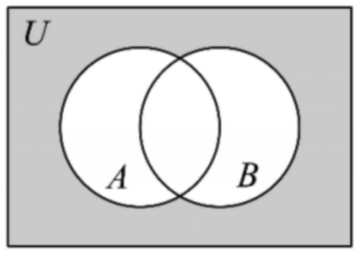
\includegraphics[width=0.20\textwidth]{figures/gao84_q9_venn.png}
\end{center}

\ifanswer
\solbegin
\step{$U=\{1,2,3,4,5,6,7,8,9,10\}$，$A=\{1,2\}$，$B=\{2,4\}$.}
\step{图中阴影部分表示的集合为 $\overline{A\cup B}=\{3,5,6,7,8,9,10\}$，共 $7$ 个元素，}
\step{其非空真子集的个数为 $2^7-2=126$.}
\solend
\fi

\item 若不等式 $ax^2-5x+c<0$ 的解集是 $(2,3)$，则不等式 $cx^2+5x+a\geqslant0$ 的解集是\blankline[4.4em].

\ifanswer
\solbegin
\step{若不等式 $ax^2-5x+c<0$ 的解集是 $(2,3)$，则 $a>0$ 且 $\begin{cases}\dfrac5a=5\\[2pt] \dfrac ca=6\end{cases}$，}
\step{则 $a=1$，$c=6$，}
\step{则不等式 $cx^2+5x+a\geqslant0$ 可化为 $6x^2+5x+1\geqslant0$，则 $x\leqslant-\dfrac12$ 或 $x\geqslant-\dfrac13$，}
\step{则不等式的解集为 $\left(-\infty,-\dfrac12\right]\cup\left[-\dfrac13,+\infty\right)$.}
\solend
\fi

\item 若关于 $x$ 的方程 $mx^2+2x+2=0$ 至少有一个负实根，则实数 $m$ 的取值范围是\blankline[4.4em].

\ifanswer
\solbegin
\step{①当 $m=0$ 时，方程为 $2x+2=0$，有一个负根，满足题意，}
\step{②当 $m\neq0$ 时，关于 $x$ 的方程 $mx^2+2x+2=0$ 至少有一个负根，}
\step{设根为 $x_1$、$x_2$，}
\step{当 $\Delta=4-8m=0$ 时，即 $m=\dfrac12$ 时，方程为 $\dfrac12x^2+2x+1=0$，}
\step{解得 $x=-2$，满足题意，}
\step{当 $\Delta=4-8m>0$，即 $m<\dfrac12$ 时，且 $m\neq0$ 时，}
\step{若有一个负根，则 $x_1x_2=\dfrac2m<0$，解得 $m<0$，}
\step{若有两个负根，则 $\begin{cases}x_1+x_2=-\dfrac2m<0\\[2pt] x_1x_2=\dfrac2m>0\end{cases}$，解得 $0<m<\dfrac12$，}
\step{综上所述，则实数 $m$ 的取值范围是 $\left(-\infty,\dfrac12\right]$.}
\solend
\fi

\item 设集合 $S$、$T$ 都至少含有两个元素，且 $S$、$T$ 同时满足：条件 1：对任意 $x$、$y\in S$，若
$x\neq y$，则 $x+y\in T$；条件 2：对任意 $x$、$y\in T$，若 $x\neq y$，则 $x-y\in S$. 给出下列说法：

①若 $S$ 只有 $2$ 个元素，则这 $2$ 个元素互为相反数；

②若 $S$ 只有 $2$ 个元素，则 $S\cup T$ 必有 $3$ 个元素；

③若 $S$ 只有 $2$ 个元素，则 $S\cup T$ 可能有 $4$ 个元素；

④存在含有 $3$ 个元素的集合 $S$，满足 $S\cup T$ 有 $4$ 个元素.

其中所有正确说法的序号是\blankline[4.4em].

\ifanswer
\solbegin
\step{对于①：由条件 2 得 $x-y\in S$，$y-x\in S$，且 $x-y\neq y-x$，}
\step{所以若 $S$ 只有 $2$ 个元素，则这 $2$ 个元素互为相反数，故①正确；}
\step{对于④：若 $S$ 有 $3$ 个元素，不妨设 $S=\{a,b,c\}$，其中 $a<b<c$，}
\step{则 $\{a+b,b+c,c+a\}\subseteq T$，所以 $c-a$、$c-b$、$b-a$、$a-c$、$b-c$、$a-b\in S$，}
\step{而 $c-a$ 与 $c-b$ 为两个互不相等的正数，$a-c$ 与 $a-b$ 为两个互不相等的负数，}
\step{故集合 $S$ 中至少有 $4$ 个元素，与 $S=\{a,b,c\}$ 有 $3$ 个元素矛盾，故④错误.}
\step{对于②③：若 $S$ 有 $2$ 个元素，由①得集合 $S$ 中的 $2$ 个元素必为相反数，}
\step{故可设 $S=\{a,-a\}(a\neq0)$. 由条件 1 得 $0\in T$，}
\step{由于集合 $T$ 中至少有 $2$ 个元素，故至少还有另外一个元素 $m\in T$.}
\step{当集合 $T$ 只有 $2$ 个元素时即 $T=\{0,m\}$，由条件 1 得 $-m\in S$，则 $m=\pm a$，}
\step{$T=\{0,a\}$ 或 $T=\{0,-a\}$，故 $S\cup T=\{0,a,-a\}$.}
\step{当集合 $T$ 有多于 $2$ 个元素时，不妨设 $T=\{0,m,n\}$，}
\step{则 $m$、$n$、$-m$、$-n$、$m-n$、$n-m\in S$，由于 $m$、$n\neq0$，}
\step{所以 $m\neq m-n$，$n\neq n-m$，又 $m\neq n$，}
\step{故集合 $S$ 至少有 $3$ 个元素，与 $S$ 中只有两个元素矛盾.}
\step{综上，$S\cup T=\{0,a,-a\}$，故②正确，③错误.}
\step{故正确的是①②.}
\solend
\fi

\end{enumerate}

\bigsec{二、选择题}

\begin{enumerate}
\setcounter{enumi}{12}

\item 用反证法证明命题：“若 $x+y>2$，则 $x>1$ 或 $y>1$”时，应假设\mbox{（\quad）}

\keepwithprev
A. $x\leqslant1$ 或 $y\leqslant1$\qquad B. 若 $x>1$ 或 $y>1$

C. $x\leqslant1$ 且 $y\leqslant1$\qquad D. 若 $x>1$ 且 $y>1$

\ifanswer
\ans{$C$}
\fi

\item 下列命题中，为真命题的是\mbox{（\quad）}

\keepwithprev
A. 若 $a>b$，则 $a^2>b^2$\qquad B. 若 $a>b$，$c>d$，则 $ac>bd$

C. 若 $a>b$，则 $\dfrac1a<\dfrac1b$\qquad D. 若 $ac^2>bc^2$，则 $a>b$

\ifanswer
\solbegin
\step{对于 $A$，当 $a=-1$，$b=-2$ 时，$a^2<b^2$，故 $A$ 错误；}
\step{对于 $B$，当 $a=-1$，$b=-2$，$c=-1$，$d=-2$ 时，$ac<bd$，故 $B$ 错误；}
\step{对于 $C$，当 $a=1$，$b=-2$ 时，$\dfrac1a>\dfrac1b$，故 $C$ 错误；}
\step{对于 $D$，因为 $ac^2-bc^2=(a-b)c^2>0$，所以 $a-b>0$，$c^2>0$，则 $a>b$，}
\step{故 $D$ 正确.}
\step{故选 $D$.}
\solend
\fi

\item 现有一级小麦 $m\,\mathrm{kg}$，二级小麦 $n\,\mathrm{kg}$，某粮食收购站有两种收购方案. 方案一：分两个
等级收购小麦，一级小麦 $a$ 元$/\mathrm{kg}$，二级小麦 $b$ 元$/\mathrm{kg}\,(b<a)$；方案二：以方案一两种价
格的平均数收购. 收购方式更加优惠的是\mbox{（\quad）}

\keepwithprev
A. 方案一\qquad B. 方案二\qquad C. 同样优惠\qquad D. 以上均有可能

\ifanswer
\solbegin
\step{方案一收购的平均价格为 $\dfrac{ma+nb}{m+n}$，方案二收购的平均价格为 $\dfrac{a+b}2$；}
\step{所以 $\dfrac{ma+nb}{m+n}-\dfrac{a+b}2=\dfrac{(a-b)(m-n)}{2(m+n)}$ ①，}
\step{$a-b>0$，$m-n$ 的正负性不确定，故①式的正负性不确定，故选 $D$.}
\solend
\fi

\item 用 $C(A)$ 表示非空集合 $A$ 中的元素个数. 对于集合 $A$、$B$，定义

$A*B=\begin{cases}C(A)-C(B),&C(A)\geqslant C(B)\\ C(B)-C(A),&C(A)<C(B)\end{cases}$，若 $A=\{0,1\}$，

$B=\{x\mid(x^2-ax)(x^2+ax+2)=0\}$，设实数 $a$ 的所有可能取值组成的集合是 $S$，则下列选
项不正确的是\mbox{（\quad）}

\keepwithprev
A. $C(B)$ 的可能值为 $1$，$2$，$3$，$4$

B. 若 $A*B=2$，则 $a$ 的取值范围为 $(-\infty,-2\sqrt2)\cup(2\sqrt2,+\infty)$

C. 若 $A*B=1$，则 $C(S)=3$

D. 若 $A*B=0$，则 $a$ 的取值范围为 $(-2\sqrt2,2\sqrt2)$

\ifanswer
\solbegin
\step{对于集合 $B$，当 $a=0$ 时，方程 $x^2(x^2+2)=0$ 的解为 $x=0$，$C(B)=1$，}
\step{当 $a\neq0$ 时，$x^2-ax=0$ 或 $x^2+ax+2=0$，}
\step{其中 $x^2-ax=0$ 的解为 $x_1=0$，$x_2=a$，}
\step{若 $\Delta=a^2-8>0$，即 $a>2\sqrt2$ 或 $a<-2\sqrt2$，}
\step{方程 $x^2+ax+2=0$ 有两个不相等的实数根，此时 $C(B)=4$；}
\step{若 $\Delta=a^2-8=0$，即 $a=2\sqrt2$ 或 $-2\sqrt2$，}
\step{方程 $x^2+ax+2=0$ 有两个相等的实数根，此时 $C(B)=3$；}
\step{若 $\Delta=a^2-8<0$，即 $-2\sqrt2<a<0$ 或 $0<a<2\sqrt2$，}
\step{方程 $x^2+ax+2=0$ 无实数根，此时 $C(B)=2$；}
\step{所以 $C(B)$ 的可能值为 $1$，$2$，$3$，$4$，故 $A$ 正确；}
\step{若 $A*B=2$，且 $C(A)=2$，则 $C(B)=4$，}
\step{则 $a$ 的取值范围 $(-\infty,-2\sqrt2)\cup(2\sqrt2,+\infty)$，故 $B$ 正确；}
\step{若 $A*B=1$，且 $C(A)=2$，则 $C(B)=1$ 或 $3$，}
\step{当 $C(B)=1$ 时，$a=0$，}
\step{当 $C(B)=3$ 时，$a=2\sqrt2$ 或 $-2\sqrt2$，此时集合 $S=\{0,-2\sqrt2,2\sqrt2\}$，}
\step{则 $C(S)=3$，故 $C$ 正确；}
\step{若 $A*B=0$，且 $C(A)=2$，则 $C(B)=2$，}
\step{由此可得 $a$ 的取值范围为 $(-2\sqrt2,0)\cup(0,2\sqrt2)$，故 $D$ 不正确；}
\step{故选 $D$.}
\solend
\fi

\end{enumerate}

\bigsec{三、解答题}

\begin{enumerate}
\setcounter{enumi}{16}

\item 已知集合 $A=\{x\mid-3<x\leqslant4\}$，集合 $B=\{x\mid k+1\leqslant x\leqslant2k-1\}$.

（1）当 $k=3$ 时，求 $A\cup B$、$\overline A\cap B$；

（2）若 $B\subseteq A$，求 $k$ 的取值范围.

\ansspace*[10]

\ifanswer
\solbegin
\stepm{（1）}{当 $k=3$ 时，$B=\{x\mid4\leqslant x\leqslant5\}$，又 $A=\{x\mid-3<x\leqslant4\}$，}
\step{所以 $\overline A=\{x\mid x\leqslant-3$ 或 $x>4\}$，}
\step{所以 $A\cup B=\{x\mid-3<x\leqslant5\}$，$\overline A\cap B=\{x\mid4<x\leqslant5\}$.}
\stepm{（2）}{①当 $B=\varnothing$，即 $k+1>2k-1$ 时，$k<2$，满足 $B\subseteq A$.}
\step{②当 $B\neq\varnothing$ 时，由 $B\subseteq A$ 得 $\begin{cases}k+1\leqslant2k-1\\ k+1>-3\\ 2k-1\leqslant4\end{cases}$，解得 $2\leqslant k\leqslant\dfrac52$，}
\step{综合①②得 $k$ 的取值范围 $\left\{k\mid k\leqslant\dfrac52\right\}$.}
\solend
\fi

\item 设集合 $A=\{x\mid x^2-3x+2=0\}$，$B=\{x\mid x^2+2(a+1)x+a^2-5=0\}$.

（1）若 $A\cap B=\{2\}$，求实数 $a$ 的值；

（2）若集合 $B$ 中有两个元素 $x_1,x_2$，求 $\lvert x_1-x_2\rvert$（用 $a$ 表示）.

\ansspace*[10]

\ifanswer
\solbegin
\stepm{（1）}{由题意得 $A=\{x\mid x^2-3x+2=0\}=\{1,2\}$，因为 $A\cap B=\{2\}$，所以 $2\in B$，}
\step{所以 $2^2+4(a+1)+a^2-5=0$ 即 $4+4a+4+a^2-5=0$，}
\step{化简得 $a^2+4a+3=0$，即 $(a+3)(a+1)=0$，解得 $a=-3$ 或 $a=-1$，}
\step{检验：当 $a=-3$ 时，$B=\{x\mid x^2-4x+4=0\}=\{2\}$，满足 $A\cap B=\{2\}$，}
\step{当 $a=-1$ 时，$B=\{x\mid x^2-4=0\}=\{-2,2\}$，满足 $A\cap B=\{2\}$，}
\step{所以 $a=-3$ 或 $a=-1$.}
\stepm{（2）}{因为 $B$ 中有两个元素 $x_1,x_2$，所以 $x^2+2(a+1)x+(a^2-5)=0$ 有两个根，}
\step{所以 $\Delta=4(a+1)^2-4(a^2-5)=8a+24>0$，}
\step{且 $x_1+x_2=-2(a+1)$，$x_1x_2=a^2-5$，}
\step{所以 $\lvert x_1-x_2\rvert=\sqrt{(x_1+x_2)^2-4x_1x_2}=\sqrt{4(a+1)^2-4(a^2-5)}=\sqrt{8a+24}$.}
\solend
\fi

\item 已知关于 $x$ 的不等式 $\dfrac{ax-2}{1+x}>0$.

（1）若 $x=-a$ 时，不等式成立，求实数 $a$ 的取值范围；

（2）若 $a$ 为实数，解关于 $x$ 的不等式：$\dfrac{ax-2}{1+x}>0$.

\ansspace*[12]

\ifanswer
\solbegin
\stepm{（1）}{因为 $x=-a$ 时，不等式成立，}
\step{所以 $\dfrac{-a^2-2}{1-a}>0\Rightarrow\dfrac{a^2+2}{a-1}>0\Rightarrow a-1>0\Rightarrow a>1$，}
\step{所以实数 $a$ 的取值范围为 $(1,+\infty)$.}
\stepm{（2）}{$\dfrac{ax-2}{1+x}>0\Rightarrow(ax-2)(x+1)>0$，}
\step{当 $a=0$ 时，$-2(x+1)>0$，解得 $x<-1$.}
\step{当 $a>0$ 时，$(ax-2)(x+1)>0$，解得 $x>\dfrac2a$ 或 $x<-1$.}
\step{当 $a<0$ 时，不等式 $(ax-2)(x+1)>0$ 可化为 $\left(x-\dfrac2a\right)(x+1)<0$，}
\step{当 $\dfrac2a>-1$，即 $a<-2$ 时，解得 $-1<x<\dfrac2a$；}
\step{当 $\dfrac2a<-1$，即 $-2<a<0$ 时，解得 $\dfrac2a<x<-1$；}
\step{当 $\dfrac2a=-1$，即 $a=-2$ 时，解集为 $\varnothing$.}
\step{综上，当 $a<-2$ 时，不等式的解集为 $\left(-1,\dfrac2a\right)$；}
\step{当 $a=-2$ 时，不等式的解集为 $\varnothing$；}
\step{当 $-2<a<0$ 时，不等式的解集为 $\left(\dfrac2a,-1\right)$；}
\step{当 $a=0$ 时，不等式的解集为 $(-\infty,-1)$；}
\step{当 $a>0$ 时，不等式的解集为 $(-\infty,-1)\cup\left(\dfrac2a,+\infty\right)$.}
\solend
\fi

\item 已知关于 $x$ 的不等式 $(k^2-2k-3)x^2+(k+1)x+1>0\,(k\in\R)$ 的解集为 $M$；

（1）若存在实数 $a$，使得 $M=(-\infty,a)\cup(a,+\infty)$，求 $k$ 的值；

（2）若 $M=\R$，求 $k$ 的取值范围；

（3）是否存在实数 $k$，满足：“对于任意 $n\in\N$，$n>0$，都有 $n\in M$；对于任意
$m\in\Z$，$m<0$，都有 $m\notin M$”，若存在，求出 $k$ 的值，若不存在，说明理由.

\ansspace*[13]

\ifanswer
\solbegin
\stepm{（1）}{记 $f(x)=(k^2-2k-3)x^2+(k+1)x+1$.}
\step{$M=(-\infty,a)\cup(a,+\infty)$ 表示 $f(x)>0$ 对一切 $x\neq a$ 成立，且 $f(a)=0$，}
\step{故需二次项系数大于 $0$ 且 $\Delta=0$.}
\step{由 $\Delta=(k+1)^2-4(k^2-2k-3)=-3k^2+10k+13=0$ 得 $k=\dfrac{13}3$ 或 $k=-1$.}
\step{当 $k=\dfrac{13}3$ 时，二次项系数 $\dfrac{64}9>0$，$f(x)=\dfrac{64}9\left(x+\dfrac38\right)^2$，符合；}
\step{当 $k=-1$ 时二次项系数为 $0$，$f(x)=1>0$，$M=\R$，不符合. 故 $k=\dfrac{13}3$.}
\stepm{（2）}{$M=\R$ 即 $f(x)>0$ 对一切 $x\in\R$ 恒成立.}
\step{①当 $k^2-2k-3>0$（即 $k<-1$ 或 $k>3$）时，需 $\Delta<0$，}
\step{即 $-3k^2+10k+13<0$，得 $k<-1$ 或 $k>\dfrac{13}3$，故 $k<-1$ 或 $k>\dfrac{13}3$；}
\step{②当 $k^2-2k-3=0$ 时，$k=3$ 得 $f(x)=4x+1$ 不恒正，不符合题意，}
\step{舍去，}
\step{当 $k=-1$ 得 $f(x)=1>0$ 恒成立，符合题意；}
\step{③当 $k^2-2k-3<0$ 时，抛物线开口向下，不能恒正.}
\step{综上，$k\leqslant-1$ 或 $k>\dfrac{13}3$.}
\stepm{（3）}{存在，$k=3$，理由如下，}
\step{由题意得解集 $M=(t,+\infty)$，$t\in[-1,1)$；}
\step{当 $k^2-2k-3=0$ 时，解得 $k=3$ 或 $k=-1$，}
\step{$k=3$ 时，不等式的解集为 $\left(-\dfrac14,+\infty\right)$，满足条件；}
\step{$k=-1$ 时，$1>0$ 恒成立，不满足条件；}
\step{当 $k^2-2k-3>0$ 时，}
\step{此时对应的一元二次不等式的解集形式不是 $(t,+\infty)$ 的形式，不满足条件；}
\step{当 $k^2-2k-3<0$ 时，}
\step{此时对应的一元二次不等式的解集形式不是 $(t,+\infty)$ 的形式，不满足条件；}
\step{综上，满足条件 $k$ 的值为 $3$.}
\solend
\fi

\item 已知有限集 $A=\{a_1,a_2,\cdots,a_n\}\,(n\geqslant2,n\in\N)$，如果 $A$ 中元素 $a_i\,(i=1,2,3,\cdots,n)$ 满足
$a_1+a_2+a_3+\cdots+a_n=a_1\times a_2\times\cdots\times a_n$，就称 $A$ 为“和积平衡集”.

（1）判断集合 $\{-1+\sqrt3,-1-\sqrt3\}$ 是否为“和积平衡集”；

（2）若 $a_1$、$a_2$ 是两个不同的正数，且 $\{a_1,a_2\}$ 是“和积平衡集”，写出以 $a_1$、$a_2$ 为根的一
个一元二次方程（系数可用 $a_1$、$a_2$ 表示），并证明 $a_1$、$a_2$ 至少有一个大于 $2$；

（3）若 $a_i\in\Z$ 且 $a_i>0$，求所有符合条件的“和积平衡集”.

\ansspace*[14]

\ifanswer
\solbegin
\stepm{（1）}{对于集合 $\{-1+\sqrt3,-1-\sqrt3\}$，}
\step{因为 $(-1+\sqrt3)+(-1-\sqrt3)=-2$，$(-1+\sqrt3)\times(-1-\sqrt3)=-2$，}
\step{所以满足 $a_1+a_2=a_1\times a_2$，满足题意，}
\step{所以集合 $\{-1+\sqrt3,-1-\sqrt3\}$ 是和积平衡集.}
\stepm{（2）}{以 $a_1$、$a_2$ 为根的一个一元二次方程可为 $x^2-(a_1+a_2)x+a_1\cdot a_2=0$，}
\step{因为 $a_1$、$a_2$ 是两个不同的正数，且 $\{a_1,a_2\}$ 是和积平衡集，}
\step{所以 $a_1+a_2=a_1\cdot a_2$，}
\step{又 $a_1$ 和 $a_2$ 为 $x^2-(a_1+a_2)x+a_1\cdot a_2=0$ 的两个不同的正根，}
\step{所以 $\Delta=(a_1+a_2)^2-4a_1a_2=(a_1+a_2)^2-4(a_1+a_2)>0$，}
\step{又 $a_1+a_2>0$，则 $a_1+a_2>4$，}
\step{若 $a_1$、$a_2$ 都小于等于 $2$，则 $a_1+a_2\leqslant4$，矛盾，}
\step{所以 $a_1$、$a_2$ 至少有一个大于 $2$；}
\stepm{（3）}{设 $A$ 中的 $a_1<a_2<a_3<\cdots<a_n$，且 $a_i\in\N^*$，}
\step{由 $a_1+a_2+a_3+\cdots+a_n=a_1\times a_2\times\cdots\times a_n$，得 $n=2$ 时明显不满足，}
\step{所以 $n\geqslant3$，故 $a_1\times a_2\times\cdots\times a_n=a_1+a_2+a_3+\cdots+a_n\leqslant na_n$，}
\step{所以 $a_1\times a_2\times\cdots\times a_{n-1}\leqslant n$，}
\step{当 $n=3$ 时，$a_1\times a_2\leqslant3$，$a_i\in\N^*$，只能有 $a_1=1$，$a_2=2$，}
\step{由 $a_1+a_2+a_3=a_1\times a_2\times a_3$，得 $a_3=3$，此时的和积平衡集为 $\{1,2,3\}$，}
\step{当 $n\geqslant4$ 时，$a_1\times a_2\times\cdots\times a_{n-1}\geqslant(n-1)(n-2)\times\cdots\times2\times1\geqslant(n-1)(n-2)$，}
\step{又 $(n-1)(n-2)-n=n^2-4n+2=n(n-4)+2>0$，即 $(n-1)(n-2)>n$，}
\step{即 $a_1\times a_2\times\cdots\times a_{n-1}>n$，与 $a_1\times a_2\times\cdots\times a_{n-1}\leqslant n$ 矛盾，}
\step{所以 $n\geqslant4$ 不满足条件，}
\step{所以符合条件的和积平衡集有且只有 $n=3$，此时的和积平衡集为 $\{1,2,3\}$.}
\solend
\fi

\end{enumerate}

\end{document}
"
% 紧凑版：xelatex "\def\iscompact{1}% 高一84_东昌中学_10月月考.tex
%   —— 高一上数学“2026-2027 年东昌中学高一上 10 月月考”（讲评版）
% 试卷版：xelatex 高一84_东昌中学_10月月考.tex
% 答案版：xelatex "\def\isanswer{1}% 高一84_东昌中学_10月月考.tex
%   —— 高一上数学“2026-2027 年东昌中学高一上 10 月月考”（讲评版）
% 试卷版：xelatex 高一84_东昌中学_10月月考.tex
% 答案版：xelatex "\def\isanswer{1}% 高一84_东昌中学_10月月考.tex
%   —— 高一上数学“2026-2027 年东昌中学高一上 10 月月考”（讲评版）
% 试卷版：xelatex 高一84_东昌中学_10月月考.tex
% 答案版：xelatex "\def\isanswer{1}\input{高一84_东昌中学_10月月考.tex}"
% 紧凑版：xelatex "\def\iscompact{1}\input{高一84_东昌中学_10月月考.tex}"
%
% 原始材料：微信公众号“魔都数学加油站”文章，连载“27学年高一84”；
% 原文标题“27学年高一84——2026-2027年上海市东昌中学高一上10月月考”；
% 原文链接：https://mp.weixin.qq.com/s/PErsjO3N5RsMuJC69IGbrw。
% 页面标注发布时间 2026-10-26 20:15（上海）。
% 正文为 12 张 PNG 页（`原图/高一84_东昌中学_10月月考/01..12.png`），
% 尺寸混排（第 1—8 页为 4762×6735，第 9—12 页为 2560×3620），均按页序读取。
%
% 篇幅与题号：原卷自第 3 题起编号（第 1、2 题不在原文内）。填空题 3—12（10 题）、
% 选择题 13—16（4 题）、解答题 17—21（5 题），共 19 题。
%
% 讲评版：19 题全部印【解析】，本稿不另提 \ans{}；选择题答案在解析末句“故选 D／C／D”。
% 第 13 题的答案“C”原卷直接印在题干括号内（“（\ C\ ）”），本稿按 高一37 第 13 题／
% 高一63 第 14 题成例括号留空、另提 \ans{$C$}（该题无【解析】段）。
%
% 副标题：原卷未印副标题。本稿按内容标作“集合与常用逻辑用语、不等式”。
%
% 与原卷的排版差异：
%   ① 原卷每题下直接印【解析】，本稿按全稿惯例将解析置于答案版；
%   ② 原卷未印副标题，本稿补出；填空横线统一排 \blankline[4.4em]；
%   ③ 原卷数集记号排斜体 $R$、$Z$、$N$，本稿按全稿惯例改用 $\R$、$\Z$、$\N$；
%   ④ 第 17—21 题的子问用行内“（1）（2）（3）”段，解析中的子问标号用 \stepm；
%   ⑤ 解答题按惯例加 \ansspace；选择题括号排 \mbox{（\quad）}；
%   ⑥ 第 9 题题干右侧有一幅韦恩图，裁自原图（第 2 页）后去粉色水印、转灰度，
%      三版都出（属题干）。
%
% 行数核对：逐题数 \step/\stepm 条数，合计 157 条（Q3：2；Q4：2；Q5：3；Q6：2；
% Q7：3；Q8：6；Q9：3；Q10：4；Q11：9；Q12：17；Q14：6；Q15：3；Q16：19；
% Q17：6；Q18：10；Q19：15；Q20：24；Q21：23）；第 13 题无解析，只提 \ans{}，
% 不计入 \step 账。原卷解析的换行按语意合并，未逐行强拆。
%
\documentclass[a4paper,11pt]{article}
\usepackage{common}

\begin{document}

\examtitlest[4]{2026--2027 年东昌中学高一上 10 月月考}{集合与常用逻辑用语、不等式}

\bigsec{一、填空题}

\begin{enumerate}
\setcounter{enumi}{2}

\item 若 $a\in\R$，则“$a=2$”是“$(a-1)(a-2)=0$”的\blankline[3.6em]条件（填“充分不必要”、“必要
不充分”、“充要”、“既不充分又不必要”的一个）.

\ifanswer
\solbegin
\step{$a=2\Rightarrow(a-1)(a-2)=0$，而 $(a-1)(a-2)=0$ 不能推出 $a=2$，}
\step{故“$a=2$”是“$(a-1)(a-2)=0$”的充分不必要条件.}
\solend
\fi

\item 已知集合 $M=\{(x,y)\mid y=x^2\}$，$N=\{(x,y)\mid y=1\}$，则 $M\cap N=\blankline[4.4em]$.

\ifanswer
\solbegin
\step{集合 $M=\{(x,y)\mid y=x^2\}$，$N=\{(x,y)\mid y=1\}$，}
\step{当 $y=1$ 时，$x=\pm1$，则 $M\cap N=\{(-1,1),(1,1)\}$.}
\solend
\fi

\item 已知集合 $A=\{x\mid x^2+ax+4=0\}$，若 $A$ 有且只有一个非空子集，则实数 $a=\blankline[4.4em]$.

\ifanswer
\solbegin
\step{因为集合 $A$ 有且只有一个非空子集，所以集合 $A$ 中只有一个元素，}
\step{所以一元二次方程 $x^2+ax+4=0$ 有两个相等的解，}
\step{所以 $\Delta=a^2-4\times4=0$，解得 $a=\pm4$.}
\solend
\fi

\item 已知 $A=(-\infty,a]$，$B=(-\infty,3)$，且 $x\in A$ 是 $x\in B$ 的充分不必要条件，则 $a$ 的取值范围
是\blankline[4.4em].

\ifanswer
\solbegin
\step{$A=(-\infty,a]$，$B=(-\infty,3)$，且 $x\in A$ 是 $x\in B$ 的充分不必要条件，}
\step{则 $A\subset B$，则 $a<3$，即 $a$ 的取值范围为 $(-\infty,3)$.}
\solend
\fi

\item 不等式 $\dfrac{3x-1}{x-2}\leqslant1$ 的解集为\blankline[4.4em].

\ifanswer
\solbegin
\step{由 $\dfrac{3x-1}{x-2}\leqslant1$，得 $\dfrac{3x-1}{x-2}-1=\dfrac{3x-1-(x-2)}{x-2}=\dfrac{2x+1}{x-2}\leqslant0$，}
\step{则 $\begin{cases}(2x+1)(x-2)\leqslant0\\ x-2\neq0\end{cases}$，解得 $-\dfrac12\leqslant x<2$，}
\step{则不等式 $\dfrac{3x-1}{x-2}\leqslant1$ 的解集为 $\left[-\dfrac12,2\right)$.}
\solend
\fi

\item 已知关于 $x$ 的一元二次方程 $x^2-2mx+(3m+1)=0$ 的两个实数根为 $x_1$、$x_2$，且
$x_1^2+x_2^2=16$，则实数 $m$ 的值为\blankline[4.4em].

\ifanswer
\solbegin
\step{由韦达定理，得 $x_1+x_2=2m$，$x_1x_2=3m+1$，}
\step{$x_1^2+x_2^2=(x_1+x_2)^2-2x_1x_2=4m^2-6m-2$，}
\step{由 $x_1^2+x_2^2=16$，得 $4m^2-6m-2=16$，即 $2m^2-3m-9=0$，}
\step{解得 $m=3$ 或 $m=-\dfrac32$，}
\step{检验判别式 $\Delta=4m^2-12m-4$，当 $m=3$ 时，$\Delta=-4<0$，舍去；}
\step{当 $m=-\dfrac32$ 时，$\Delta=23>0$，符合条件，故 $m=-\dfrac32$.}
\solend
\fi

\item 已知全集 $U=\{x\mid1\leqslant x\leqslant10,\,x\in\N\}$，集合 $A=\{x\mid x^2-3<4,\,x\in\N,\,x>0\}$，
$B=\{2,4\}$，则图中阴影部分表示的集合的非空真子集个数为\blankline[4.4em].

\needvspace{9\baselineskip}
\begin{center}
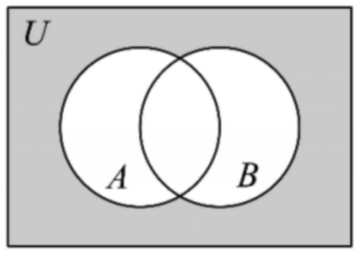
\includegraphics[width=0.20\textwidth]{figures/gao84_q9_venn.png}
\end{center}

\ifanswer
\solbegin
\step{$U=\{1,2,3,4,5,6,7,8,9,10\}$，$A=\{1,2\}$，$B=\{2,4\}$.}
\step{图中阴影部分表示的集合为 $\overline{A\cup B}=\{3,5,6,7,8,9,10\}$，共 $7$ 个元素，}
\step{其非空真子集的个数为 $2^7-2=126$.}
\solend
\fi

\item 若不等式 $ax^2-5x+c<0$ 的解集是 $(2,3)$，则不等式 $cx^2+5x+a\geqslant0$ 的解集是\blankline[4.4em].

\ifanswer
\solbegin
\step{若不等式 $ax^2-5x+c<0$ 的解集是 $(2,3)$，则 $a>0$ 且 $\begin{cases}\dfrac5a=5\\[2pt] \dfrac ca=6\end{cases}$，}
\step{则 $a=1$，$c=6$，}
\step{则不等式 $cx^2+5x+a\geqslant0$ 可化为 $6x^2+5x+1\geqslant0$，则 $x\leqslant-\dfrac12$ 或 $x\geqslant-\dfrac13$，}
\step{则不等式的解集为 $\left(-\infty,-\dfrac12\right]\cup\left[-\dfrac13,+\infty\right)$.}
\solend
\fi

\item 若关于 $x$ 的方程 $mx^2+2x+2=0$ 至少有一个负实根，则实数 $m$ 的取值范围是\blankline[4.4em].

\ifanswer
\solbegin
\step{①当 $m=0$ 时，方程为 $2x+2=0$，有一个负根，满足题意，}
\step{②当 $m\neq0$ 时，关于 $x$ 的方程 $mx^2+2x+2=0$ 至少有一个负根，}
\step{设根为 $x_1$、$x_2$，}
\step{当 $\Delta=4-8m=0$ 时，即 $m=\dfrac12$ 时，方程为 $\dfrac12x^2+2x+1=0$，}
\step{解得 $x=-2$，满足题意，}
\step{当 $\Delta=4-8m>0$，即 $m<\dfrac12$ 时，且 $m\neq0$ 时，}
\step{若有一个负根，则 $x_1x_2=\dfrac2m<0$，解得 $m<0$，}
\step{若有两个负根，则 $\begin{cases}x_1+x_2=-\dfrac2m<0\\[2pt] x_1x_2=\dfrac2m>0\end{cases}$，解得 $0<m<\dfrac12$，}
\step{综上所述，则实数 $m$ 的取值范围是 $\left(-\infty,\dfrac12\right]$.}
\solend
\fi

\item 设集合 $S$、$T$ 都至少含有两个元素，且 $S$、$T$ 同时满足：条件 1：对任意 $x$、$y\in S$，若
$x\neq y$，则 $x+y\in T$；条件 2：对任意 $x$、$y\in T$，若 $x\neq y$，则 $x-y\in S$. 给出下列说法：

①若 $S$ 只有 $2$ 个元素，则这 $2$ 个元素互为相反数；

②若 $S$ 只有 $2$ 个元素，则 $S\cup T$ 必有 $3$ 个元素；

③若 $S$ 只有 $2$ 个元素，则 $S\cup T$ 可能有 $4$ 个元素；

④存在含有 $3$ 个元素的集合 $S$，满足 $S\cup T$ 有 $4$ 个元素.

其中所有正确说法的序号是\blankline[4.4em].

\ifanswer
\solbegin
\step{对于①：由条件 2 得 $x-y\in S$，$y-x\in S$，且 $x-y\neq y-x$，}
\step{所以若 $S$ 只有 $2$ 个元素，则这 $2$ 个元素互为相反数，故①正确；}
\step{对于④：若 $S$ 有 $3$ 个元素，不妨设 $S=\{a,b,c\}$，其中 $a<b<c$，}
\step{则 $\{a+b,b+c,c+a\}\subseteq T$，所以 $c-a$、$c-b$、$b-a$、$a-c$、$b-c$、$a-b\in S$，}
\step{而 $c-a$ 与 $c-b$ 为两个互不相等的正数，$a-c$ 与 $a-b$ 为两个互不相等的负数，}
\step{故集合 $S$ 中至少有 $4$ 个元素，与 $S=\{a,b,c\}$ 有 $3$ 个元素矛盾，故④错误.}
\step{对于②③：若 $S$ 有 $2$ 个元素，由①得集合 $S$ 中的 $2$ 个元素必为相反数，}
\step{故可设 $S=\{a,-a\}(a\neq0)$. 由条件 1 得 $0\in T$，}
\step{由于集合 $T$ 中至少有 $2$ 个元素，故至少还有另外一个元素 $m\in T$.}
\step{当集合 $T$ 只有 $2$ 个元素时即 $T=\{0,m\}$，由条件 1 得 $-m\in S$，则 $m=\pm a$，}
\step{$T=\{0,a\}$ 或 $T=\{0,-a\}$，故 $S\cup T=\{0,a,-a\}$.}
\step{当集合 $T$ 有多于 $2$ 个元素时，不妨设 $T=\{0,m,n\}$，}
\step{则 $m$、$n$、$-m$、$-n$、$m-n$、$n-m\in S$，由于 $m$、$n\neq0$，}
\step{所以 $m\neq m-n$，$n\neq n-m$，又 $m\neq n$，}
\step{故集合 $S$ 至少有 $3$ 个元素，与 $S$ 中只有两个元素矛盾.}
\step{综上，$S\cup T=\{0,a,-a\}$，故②正确，③错误.}
\step{故正确的是①②.}
\solend
\fi

\end{enumerate}

\bigsec{二、选择题}

\begin{enumerate}
\setcounter{enumi}{12}

\item 用反证法证明命题：“若 $x+y>2$，则 $x>1$ 或 $y>1$”时，应假设\mbox{（\quad）}

\keepwithprev
A. $x\leqslant1$ 或 $y\leqslant1$\qquad B. 若 $x>1$ 或 $y>1$

C. $x\leqslant1$ 且 $y\leqslant1$\qquad D. 若 $x>1$ 且 $y>1$

\ifanswer
\ans{$C$}
\fi

\item 下列命题中，为真命题的是\mbox{（\quad）}

\keepwithprev
A. 若 $a>b$，则 $a^2>b^2$\qquad B. 若 $a>b$，$c>d$，则 $ac>bd$

C. 若 $a>b$，则 $\dfrac1a<\dfrac1b$\qquad D. 若 $ac^2>bc^2$，则 $a>b$

\ifanswer
\solbegin
\step{对于 $A$，当 $a=-1$，$b=-2$ 时，$a^2<b^2$，故 $A$ 错误；}
\step{对于 $B$，当 $a=-1$，$b=-2$，$c=-1$，$d=-2$ 时，$ac<bd$，故 $B$ 错误；}
\step{对于 $C$，当 $a=1$，$b=-2$ 时，$\dfrac1a>\dfrac1b$，故 $C$ 错误；}
\step{对于 $D$，因为 $ac^2-bc^2=(a-b)c^2>0$，所以 $a-b>0$，$c^2>0$，则 $a>b$，}
\step{故 $D$ 正确.}
\step{故选 $D$.}
\solend
\fi

\item 现有一级小麦 $m\,\mathrm{kg}$，二级小麦 $n\,\mathrm{kg}$，某粮食收购站有两种收购方案. 方案一：分两个
等级收购小麦，一级小麦 $a$ 元$/\mathrm{kg}$，二级小麦 $b$ 元$/\mathrm{kg}\,(b<a)$；方案二：以方案一两种价
格的平均数收购. 收购方式更加优惠的是\mbox{（\quad）}

\keepwithprev
A. 方案一\qquad B. 方案二\qquad C. 同样优惠\qquad D. 以上均有可能

\ifanswer
\solbegin
\step{方案一收购的平均价格为 $\dfrac{ma+nb}{m+n}$，方案二收购的平均价格为 $\dfrac{a+b}2$；}
\step{所以 $\dfrac{ma+nb}{m+n}-\dfrac{a+b}2=\dfrac{(a-b)(m-n)}{2(m+n)}$ ①，}
\step{$a-b>0$，$m-n$ 的正负性不确定，故①式的正负性不确定，故选 $D$.}
\solend
\fi

\item 用 $C(A)$ 表示非空集合 $A$ 中的元素个数. 对于集合 $A$、$B$，定义

$A*B=\begin{cases}C(A)-C(B),&C(A)\geqslant C(B)\\ C(B)-C(A),&C(A)<C(B)\end{cases}$，若 $A=\{0,1\}$，

$B=\{x\mid(x^2-ax)(x^2+ax+2)=0\}$，设实数 $a$ 的所有可能取值组成的集合是 $S$，则下列选
项不正确的是\mbox{（\quad）}

\keepwithprev
A. $C(B)$ 的可能值为 $1$，$2$，$3$，$4$

B. 若 $A*B=2$，则 $a$ 的取值范围为 $(-\infty,-2\sqrt2)\cup(2\sqrt2,+\infty)$

C. 若 $A*B=1$，则 $C(S)=3$

D. 若 $A*B=0$，则 $a$ 的取值范围为 $(-2\sqrt2,2\sqrt2)$

\ifanswer
\solbegin
\step{对于集合 $B$，当 $a=0$ 时，方程 $x^2(x^2+2)=0$ 的解为 $x=0$，$C(B)=1$，}
\step{当 $a\neq0$ 时，$x^2-ax=0$ 或 $x^2+ax+2=0$，}
\step{其中 $x^2-ax=0$ 的解为 $x_1=0$，$x_2=a$，}
\step{若 $\Delta=a^2-8>0$，即 $a>2\sqrt2$ 或 $a<-2\sqrt2$，}
\step{方程 $x^2+ax+2=0$ 有两个不相等的实数根，此时 $C(B)=4$；}
\step{若 $\Delta=a^2-8=0$，即 $a=2\sqrt2$ 或 $-2\sqrt2$，}
\step{方程 $x^2+ax+2=0$ 有两个相等的实数根，此时 $C(B)=3$；}
\step{若 $\Delta=a^2-8<0$，即 $-2\sqrt2<a<0$ 或 $0<a<2\sqrt2$，}
\step{方程 $x^2+ax+2=0$ 无实数根，此时 $C(B)=2$；}
\step{所以 $C(B)$ 的可能值为 $1$，$2$，$3$，$4$，故 $A$ 正确；}
\step{若 $A*B=2$，且 $C(A)=2$，则 $C(B)=4$，}
\step{则 $a$ 的取值范围 $(-\infty,-2\sqrt2)\cup(2\sqrt2,+\infty)$，故 $B$ 正确；}
\step{若 $A*B=1$，且 $C(A)=2$，则 $C(B)=1$ 或 $3$，}
\step{当 $C(B)=1$ 时，$a=0$，}
\step{当 $C(B)=3$ 时，$a=2\sqrt2$ 或 $-2\sqrt2$，此时集合 $S=\{0,-2\sqrt2,2\sqrt2\}$，}
\step{则 $C(S)=3$，故 $C$ 正确；}
\step{若 $A*B=0$，且 $C(A)=2$，则 $C(B)=2$，}
\step{由此可得 $a$ 的取值范围为 $(-2\sqrt2,0)\cup(0,2\sqrt2)$，故 $D$ 不正确；}
\step{故选 $D$.}
\solend
\fi

\end{enumerate}

\bigsec{三、解答题}

\begin{enumerate}
\setcounter{enumi}{16}

\item 已知集合 $A=\{x\mid-3<x\leqslant4\}$，集合 $B=\{x\mid k+1\leqslant x\leqslant2k-1\}$.

（1）当 $k=3$ 时，求 $A\cup B$、$\overline A\cap B$；

（2）若 $B\subseteq A$，求 $k$ 的取值范围.

\ansspace*[10]

\ifanswer
\solbegin
\stepm{（1）}{当 $k=3$ 时，$B=\{x\mid4\leqslant x\leqslant5\}$，又 $A=\{x\mid-3<x\leqslant4\}$，}
\step{所以 $\overline A=\{x\mid x\leqslant-3$ 或 $x>4\}$，}
\step{所以 $A\cup B=\{x\mid-3<x\leqslant5\}$，$\overline A\cap B=\{x\mid4<x\leqslant5\}$.}
\stepm{（2）}{①当 $B=\varnothing$，即 $k+1>2k-1$ 时，$k<2$，满足 $B\subseteq A$.}
\step{②当 $B\neq\varnothing$ 时，由 $B\subseteq A$ 得 $\begin{cases}k+1\leqslant2k-1\\ k+1>-3\\ 2k-1\leqslant4\end{cases}$，解得 $2\leqslant k\leqslant\dfrac52$，}
\step{综合①②得 $k$ 的取值范围 $\left\{k\mid k\leqslant\dfrac52\right\}$.}
\solend
\fi

\item 设集合 $A=\{x\mid x^2-3x+2=0\}$，$B=\{x\mid x^2+2(a+1)x+a^2-5=0\}$.

（1）若 $A\cap B=\{2\}$，求实数 $a$ 的值；

（2）若集合 $B$ 中有两个元素 $x_1,x_2$，求 $\lvert x_1-x_2\rvert$（用 $a$ 表示）.

\ansspace*[10]

\ifanswer
\solbegin
\stepm{（1）}{由题意得 $A=\{x\mid x^2-3x+2=0\}=\{1,2\}$，因为 $A\cap B=\{2\}$，所以 $2\in B$，}
\step{所以 $2^2+4(a+1)+a^2-5=0$ 即 $4+4a+4+a^2-5=0$，}
\step{化简得 $a^2+4a+3=0$，即 $(a+3)(a+1)=0$，解得 $a=-3$ 或 $a=-1$，}
\step{检验：当 $a=-3$ 时，$B=\{x\mid x^2-4x+4=0\}=\{2\}$，满足 $A\cap B=\{2\}$，}
\step{当 $a=-1$ 时，$B=\{x\mid x^2-4=0\}=\{-2,2\}$，满足 $A\cap B=\{2\}$，}
\step{所以 $a=-3$ 或 $a=-1$.}
\stepm{（2）}{因为 $B$ 中有两个元素 $x_1,x_2$，所以 $x^2+2(a+1)x+(a^2-5)=0$ 有两个根，}
\step{所以 $\Delta=4(a+1)^2-4(a^2-5)=8a+24>0$，}
\step{且 $x_1+x_2=-2(a+1)$，$x_1x_2=a^2-5$，}
\step{所以 $\lvert x_1-x_2\rvert=\sqrt{(x_1+x_2)^2-4x_1x_2}=\sqrt{4(a+1)^2-4(a^2-5)}=\sqrt{8a+24}$.}
\solend
\fi

\item 已知关于 $x$ 的不等式 $\dfrac{ax-2}{1+x}>0$.

（1）若 $x=-a$ 时，不等式成立，求实数 $a$ 的取值范围；

（2）若 $a$ 为实数，解关于 $x$ 的不等式：$\dfrac{ax-2}{1+x}>0$.

\ansspace*[12]

\ifanswer
\solbegin
\stepm{（1）}{因为 $x=-a$ 时，不等式成立，}
\step{所以 $\dfrac{-a^2-2}{1-a}>0\Rightarrow\dfrac{a^2+2}{a-1}>0\Rightarrow a-1>0\Rightarrow a>1$，}
\step{所以实数 $a$ 的取值范围为 $(1,+\infty)$.}
\stepm{（2）}{$\dfrac{ax-2}{1+x}>0\Rightarrow(ax-2)(x+1)>0$，}
\step{当 $a=0$ 时，$-2(x+1)>0$，解得 $x<-1$.}
\step{当 $a>0$ 时，$(ax-2)(x+1)>0$，解得 $x>\dfrac2a$ 或 $x<-1$.}
\step{当 $a<0$ 时，不等式 $(ax-2)(x+1)>0$ 可化为 $\left(x-\dfrac2a\right)(x+1)<0$，}
\step{当 $\dfrac2a>-1$，即 $a<-2$ 时，解得 $-1<x<\dfrac2a$；}
\step{当 $\dfrac2a<-1$，即 $-2<a<0$ 时，解得 $\dfrac2a<x<-1$；}
\step{当 $\dfrac2a=-1$，即 $a=-2$ 时，解集为 $\varnothing$.}
\step{综上，当 $a<-2$ 时，不等式的解集为 $\left(-1,\dfrac2a\right)$；}
\step{当 $a=-2$ 时，不等式的解集为 $\varnothing$；}
\step{当 $-2<a<0$ 时，不等式的解集为 $\left(\dfrac2a,-1\right)$；}
\step{当 $a=0$ 时，不等式的解集为 $(-\infty,-1)$；}
\step{当 $a>0$ 时，不等式的解集为 $(-\infty,-1)\cup\left(\dfrac2a,+\infty\right)$.}
\solend
\fi

\item 已知关于 $x$ 的不等式 $(k^2-2k-3)x^2+(k+1)x+1>0\,(k\in\R)$ 的解集为 $M$；

（1）若存在实数 $a$，使得 $M=(-\infty,a)\cup(a,+\infty)$，求 $k$ 的值；

（2）若 $M=\R$，求 $k$ 的取值范围；

（3）是否存在实数 $k$，满足：“对于任意 $n\in\N$，$n>0$，都有 $n\in M$；对于任意
$m\in\Z$，$m<0$，都有 $m\notin M$”，若存在，求出 $k$ 的值，若不存在，说明理由.

\ansspace*[13]

\ifanswer
\solbegin
\stepm{（1）}{记 $f(x)=(k^2-2k-3)x^2+(k+1)x+1$.}
\step{$M=(-\infty,a)\cup(a,+\infty)$ 表示 $f(x)>0$ 对一切 $x\neq a$ 成立，且 $f(a)=0$，}
\step{故需二次项系数大于 $0$ 且 $\Delta=0$.}
\step{由 $\Delta=(k+1)^2-4(k^2-2k-3)=-3k^2+10k+13=0$ 得 $k=\dfrac{13}3$ 或 $k=-1$.}
\step{当 $k=\dfrac{13}3$ 时，二次项系数 $\dfrac{64}9>0$，$f(x)=\dfrac{64}9\left(x+\dfrac38\right)^2$，符合；}
\step{当 $k=-1$ 时二次项系数为 $0$，$f(x)=1>0$，$M=\R$，不符合. 故 $k=\dfrac{13}3$.}
\stepm{（2）}{$M=\R$ 即 $f(x)>0$ 对一切 $x\in\R$ 恒成立.}
\step{①当 $k^2-2k-3>0$（即 $k<-1$ 或 $k>3$）时，需 $\Delta<0$，}
\step{即 $-3k^2+10k+13<0$，得 $k<-1$ 或 $k>\dfrac{13}3$，故 $k<-1$ 或 $k>\dfrac{13}3$；}
\step{②当 $k^2-2k-3=0$ 时，$k=3$ 得 $f(x)=4x+1$ 不恒正，不符合题意，}
\step{舍去，}
\step{当 $k=-1$ 得 $f(x)=1>0$ 恒成立，符合题意；}
\step{③当 $k^2-2k-3<0$ 时，抛物线开口向下，不能恒正.}
\step{综上，$k\leqslant-1$ 或 $k>\dfrac{13}3$.}
\stepm{（3）}{存在，$k=3$，理由如下，}
\step{由题意得解集 $M=(t,+\infty)$，$t\in[-1,1)$；}
\step{当 $k^2-2k-3=0$ 时，解得 $k=3$ 或 $k=-1$，}
\step{$k=3$ 时，不等式的解集为 $\left(-\dfrac14,+\infty\right)$，满足条件；}
\step{$k=-1$ 时，$1>0$ 恒成立，不满足条件；}
\step{当 $k^2-2k-3>0$ 时，}
\step{此时对应的一元二次不等式的解集形式不是 $(t,+\infty)$ 的形式，不满足条件；}
\step{当 $k^2-2k-3<0$ 时，}
\step{此时对应的一元二次不等式的解集形式不是 $(t,+\infty)$ 的形式，不满足条件；}
\step{综上，满足条件 $k$ 的值为 $3$.}
\solend
\fi

\item 已知有限集 $A=\{a_1,a_2,\cdots,a_n\}\,(n\geqslant2,n\in\N)$，如果 $A$ 中元素 $a_i\,(i=1,2,3,\cdots,n)$ 满足
$a_1+a_2+a_3+\cdots+a_n=a_1\times a_2\times\cdots\times a_n$，就称 $A$ 为“和积平衡集”.

（1）判断集合 $\{-1+\sqrt3,-1-\sqrt3\}$ 是否为“和积平衡集”；

（2）若 $a_1$、$a_2$ 是两个不同的正数，且 $\{a_1,a_2\}$ 是“和积平衡集”，写出以 $a_1$、$a_2$ 为根的一
个一元二次方程（系数可用 $a_1$、$a_2$ 表示），并证明 $a_1$、$a_2$ 至少有一个大于 $2$；

（3）若 $a_i\in\Z$ 且 $a_i>0$，求所有符合条件的“和积平衡集”.

\ansspace*[14]

\ifanswer
\solbegin
\stepm{（1）}{对于集合 $\{-1+\sqrt3,-1-\sqrt3\}$，}
\step{因为 $(-1+\sqrt3)+(-1-\sqrt3)=-2$，$(-1+\sqrt3)\times(-1-\sqrt3)=-2$，}
\step{所以满足 $a_1+a_2=a_1\times a_2$，满足题意，}
\step{所以集合 $\{-1+\sqrt3,-1-\sqrt3\}$ 是和积平衡集.}
\stepm{（2）}{以 $a_1$、$a_2$ 为根的一个一元二次方程可为 $x^2-(a_1+a_2)x+a_1\cdot a_2=0$，}
\step{因为 $a_1$、$a_2$ 是两个不同的正数，且 $\{a_1,a_2\}$ 是和积平衡集，}
\step{所以 $a_1+a_2=a_1\cdot a_2$，}
\step{又 $a_1$ 和 $a_2$ 为 $x^2-(a_1+a_2)x+a_1\cdot a_2=0$ 的两个不同的正根，}
\step{所以 $\Delta=(a_1+a_2)^2-4a_1a_2=(a_1+a_2)^2-4(a_1+a_2)>0$，}
\step{又 $a_1+a_2>0$，则 $a_1+a_2>4$，}
\step{若 $a_1$、$a_2$ 都小于等于 $2$，则 $a_1+a_2\leqslant4$，矛盾，}
\step{所以 $a_1$、$a_2$ 至少有一个大于 $2$；}
\stepm{（3）}{设 $A$ 中的 $a_1<a_2<a_3<\cdots<a_n$，且 $a_i\in\N^*$，}
\step{由 $a_1+a_2+a_3+\cdots+a_n=a_1\times a_2\times\cdots\times a_n$，得 $n=2$ 时明显不满足，}
\step{所以 $n\geqslant3$，故 $a_1\times a_2\times\cdots\times a_n=a_1+a_2+a_3+\cdots+a_n\leqslant na_n$，}
\step{所以 $a_1\times a_2\times\cdots\times a_{n-1}\leqslant n$，}
\step{当 $n=3$ 时，$a_1\times a_2\leqslant3$，$a_i\in\N^*$，只能有 $a_1=1$，$a_2=2$，}
\step{由 $a_1+a_2+a_3=a_1\times a_2\times a_3$，得 $a_3=3$，此时的和积平衡集为 $\{1,2,3\}$，}
\step{当 $n\geqslant4$ 时，$a_1\times a_2\times\cdots\times a_{n-1}\geqslant(n-1)(n-2)\times\cdots\times2\times1\geqslant(n-1)(n-2)$，}
\step{又 $(n-1)(n-2)-n=n^2-4n+2=n(n-4)+2>0$，即 $(n-1)(n-2)>n$，}
\step{即 $a_1\times a_2\times\cdots\times a_{n-1}>n$，与 $a_1\times a_2\times\cdots\times a_{n-1}\leqslant n$ 矛盾，}
\step{所以 $n\geqslant4$ 不满足条件，}
\step{所以符合条件的和积平衡集有且只有 $n=3$，此时的和积平衡集为 $\{1,2,3\}$.}
\solend
\fi

\end{enumerate}

\end{document}
"
% 紧凑版：xelatex "\def\iscompact{1}% 高一84_东昌中学_10月月考.tex
%   —— 高一上数学“2026-2027 年东昌中学高一上 10 月月考”（讲评版）
% 试卷版：xelatex 高一84_东昌中学_10月月考.tex
% 答案版：xelatex "\def\isanswer{1}\input{高一84_东昌中学_10月月考.tex}"
% 紧凑版：xelatex "\def\iscompact{1}\input{高一84_东昌中学_10月月考.tex}"
%
% 原始材料：微信公众号“魔都数学加油站”文章，连载“27学年高一84”；
% 原文标题“27学年高一84——2026-2027年上海市东昌中学高一上10月月考”；
% 原文链接：https://mp.weixin.qq.com/s/PErsjO3N5RsMuJC69IGbrw。
% 页面标注发布时间 2026-10-26 20:15（上海）。
% 正文为 12 张 PNG 页（`原图/高一84_东昌中学_10月月考/01..12.png`），
% 尺寸混排（第 1—8 页为 4762×6735，第 9—12 页为 2560×3620），均按页序读取。
%
% 篇幅与题号：原卷自第 3 题起编号（第 1、2 题不在原文内）。填空题 3—12（10 题）、
% 选择题 13—16（4 题）、解答题 17—21（5 题），共 19 题。
%
% 讲评版：19 题全部印【解析】，本稿不另提 \ans{}；选择题答案在解析末句“故选 D／C／D”。
% 第 13 题的答案“C”原卷直接印在题干括号内（“（\ C\ ）”），本稿按 高一37 第 13 题／
% 高一63 第 14 题成例括号留空、另提 \ans{$C$}（该题无【解析】段）。
%
% 副标题：原卷未印副标题。本稿按内容标作“集合与常用逻辑用语、不等式”。
%
% 与原卷的排版差异：
%   ① 原卷每题下直接印【解析】，本稿按全稿惯例将解析置于答案版；
%   ② 原卷未印副标题，本稿补出；填空横线统一排 \blankline[4.4em]；
%   ③ 原卷数集记号排斜体 $R$、$Z$、$N$，本稿按全稿惯例改用 $\R$、$\Z$、$\N$；
%   ④ 第 17—21 题的子问用行内“（1）（2）（3）”段，解析中的子问标号用 \stepm；
%   ⑤ 解答题按惯例加 \ansspace；选择题括号排 \mbox{（\quad）}；
%   ⑥ 第 9 题题干右侧有一幅韦恩图，裁自原图（第 2 页）后去粉色水印、转灰度，
%      三版都出（属题干）。
%
% 行数核对：逐题数 \step/\stepm 条数，合计 157 条（Q3：2；Q4：2；Q5：3；Q6：2；
% Q7：3；Q8：6；Q9：3；Q10：4；Q11：9；Q12：17；Q14：6；Q15：3；Q16：19；
% Q17：6；Q18：10；Q19：15；Q20：24；Q21：23）；第 13 题无解析，只提 \ans{}，
% 不计入 \step 账。原卷解析的换行按语意合并，未逐行强拆。
%
\documentclass[a4paper,11pt]{article}
\usepackage{common}

\begin{document}

\examtitlest[4]{2026--2027 年东昌中学高一上 10 月月考}{集合与常用逻辑用语、不等式}

\bigsec{一、填空题}

\begin{enumerate}
\setcounter{enumi}{2}

\item 若 $a\in\R$，则“$a=2$”是“$(a-1)(a-2)=0$”的\blankline[3.6em]条件（填“充分不必要”、“必要
不充分”、“充要”、“既不充分又不必要”的一个）.

\ifanswer
\solbegin
\step{$a=2\Rightarrow(a-1)(a-2)=0$，而 $(a-1)(a-2)=0$ 不能推出 $a=2$，}
\step{故“$a=2$”是“$(a-1)(a-2)=0$”的充分不必要条件.}
\solend
\fi

\item 已知集合 $M=\{(x,y)\mid y=x^2\}$，$N=\{(x,y)\mid y=1\}$，则 $M\cap N=\blankline[4.4em]$.

\ifanswer
\solbegin
\step{集合 $M=\{(x,y)\mid y=x^2\}$，$N=\{(x,y)\mid y=1\}$，}
\step{当 $y=1$ 时，$x=\pm1$，则 $M\cap N=\{(-1,1),(1,1)\}$.}
\solend
\fi

\item 已知集合 $A=\{x\mid x^2+ax+4=0\}$，若 $A$ 有且只有一个非空子集，则实数 $a=\blankline[4.4em]$.

\ifanswer
\solbegin
\step{因为集合 $A$ 有且只有一个非空子集，所以集合 $A$ 中只有一个元素，}
\step{所以一元二次方程 $x^2+ax+4=0$ 有两个相等的解，}
\step{所以 $\Delta=a^2-4\times4=0$，解得 $a=\pm4$.}
\solend
\fi

\item 已知 $A=(-\infty,a]$，$B=(-\infty,3)$，且 $x\in A$ 是 $x\in B$ 的充分不必要条件，则 $a$ 的取值范围
是\blankline[4.4em].

\ifanswer
\solbegin
\step{$A=(-\infty,a]$，$B=(-\infty,3)$，且 $x\in A$ 是 $x\in B$ 的充分不必要条件，}
\step{则 $A\subset B$，则 $a<3$，即 $a$ 的取值范围为 $(-\infty,3)$.}
\solend
\fi

\item 不等式 $\dfrac{3x-1}{x-2}\leqslant1$ 的解集为\blankline[4.4em].

\ifanswer
\solbegin
\step{由 $\dfrac{3x-1}{x-2}\leqslant1$，得 $\dfrac{3x-1}{x-2}-1=\dfrac{3x-1-(x-2)}{x-2}=\dfrac{2x+1}{x-2}\leqslant0$，}
\step{则 $\begin{cases}(2x+1)(x-2)\leqslant0\\ x-2\neq0\end{cases}$，解得 $-\dfrac12\leqslant x<2$，}
\step{则不等式 $\dfrac{3x-1}{x-2}\leqslant1$ 的解集为 $\left[-\dfrac12,2\right)$.}
\solend
\fi

\item 已知关于 $x$ 的一元二次方程 $x^2-2mx+(3m+1)=0$ 的两个实数根为 $x_1$、$x_2$，且
$x_1^2+x_2^2=16$，则实数 $m$ 的值为\blankline[4.4em].

\ifanswer
\solbegin
\step{由韦达定理，得 $x_1+x_2=2m$，$x_1x_2=3m+1$，}
\step{$x_1^2+x_2^2=(x_1+x_2)^2-2x_1x_2=4m^2-6m-2$，}
\step{由 $x_1^2+x_2^2=16$，得 $4m^2-6m-2=16$，即 $2m^2-3m-9=0$，}
\step{解得 $m=3$ 或 $m=-\dfrac32$，}
\step{检验判别式 $\Delta=4m^2-12m-4$，当 $m=3$ 时，$\Delta=-4<0$，舍去；}
\step{当 $m=-\dfrac32$ 时，$\Delta=23>0$，符合条件，故 $m=-\dfrac32$.}
\solend
\fi

\item 已知全集 $U=\{x\mid1\leqslant x\leqslant10,\,x\in\N\}$，集合 $A=\{x\mid x^2-3<4,\,x\in\N,\,x>0\}$，
$B=\{2,4\}$，则图中阴影部分表示的集合的非空真子集个数为\blankline[4.4em].

\needvspace{9\baselineskip}
\begin{center}
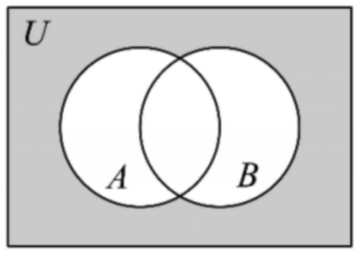
\includegraphics[width=0.20\textwidth]{figures/gao84_q9_venn.png}
\end{center}

\ifanswer
\solbegin
\step{$U=\{1,2,3,4,5,6,7,8,9,10\}$，$A=\{1,2\}$，$B=\{2,4\}$.}
\step{图中阴影部分表示的集合为 $\overline{A\cup B}=\{3,5,6,7,8,9,10\}$，共 $7$ 个元素，}
\step{其非空真子集的个数为 $2^7-2=126$.}
\solend
\fi

\item 若不等式 $ax^2-5x+c<0$ 的解集是 $(2,3)$，则不等式 $cx^2+5x+a\geqslant0$ 的解集是\blankline[4.4em].

\ifanswer
\solbegin
\step{若不等式 $ax^2-5x+c<0$ 的解集是 $(2,3)$，则 $a>0$ 且 $\begin{cases}\dfrac5a=5\\[2pt] \dfrac ca=6\end{cases}$，}
\step{则 $a=1$，$c=6$，}
\step{则不等式 $cx^2+5x+a\geqslant0$ 可化为 $6x^2+5x+1\geqslant0$，则 $x\leqslant-\dfrac12$ 或 $x\geqslant-\dfrac13$，}
\step{则不等式的解集为 $\left(-\infty,-\dfrac12\right]\cup\left[-\dfrac13,+\infty\right)$.}
\solend
\fi

\item 若关于 $x$ 的方程 $mx^2+2x+2=0$ 至少有一个负实根，则实数 $m$ 的取值范围是\blankline[4.4em].

\ifanswer
\solbegin
\step{①当 $m=0$ 时，方程为 $2x+2=0$，有一个负根，满足题意，}
\step{②当 $m\neq0$ 时，关于 $x$ 的方程 $mx^2+2x+2=0$ 至少有一个负根，}
\step{设根为 $x_1$、$x_2$，}
\step{当 $\Delta=4-8m=0$ 时，即 $m=\dfrac12$ 时，方程为 $\dfrac12x^2+2x+1=0$，}
\step{解得 $x=-2$，满足题意，}
\step{当 $\Delta=4-8m>0$，即 $m<\dfrac12$ 时，且 $m\neq0$ 时，}
\step{若有一个负根，则 $x_1x_2=\dfrac2m<0$，解得 $m<0$，}
\step{若有两个负根，则 $\begin{cases}x_1+x_2=-\dfrac2m<0\\[2pt] x_1x_2=\dfrac2m>0\end{cases}$，解得 $0<m<\dfrac12$，}
\step{综上所述，则实数 $m$ 的取值范围是 $\left(-\infty,\dfrac12\right]$.}
\solend
\fi

\item 设集合 $S$、$T$ 都至少含有两个元素，且 $S$、$T$ 同时满足：条件 1：对任意 $x$、$y\in S$，若
$x\neq y$，则 $x+y\in T$；条件 2：对任意 $x$、$y\in T$，若 $x\neq y$，则 $x-y\in S$. 给出下列说法：

①若 $S$ 只有 $2$ 个元素，则这 $2$ 个元素互为相反数；

②若 $S$ 只有 $2$ 个元素，则 $S\cup T$ 必有 $3$ 个元素；

③若 $S$ 只有 $2$ 个元素，则 $S\cup T$ 可能有 $4$ 个元素；

④存在含有 $3$ 个元素的集合 $S$，满足 $S\cup T$ 有 $4$ 个元素.

其中所有正确说法的序号是\blankline[4.4em].

\ifanswer
\solbegin
\step{对于①：由条件 2 得 $x-y\in S$，$y-x\in S$，且 $x-y\neq y-x$，}
\step{所以若 $S$ 只有 $2$ 个元素，则这 $2$ 个元素互为相反数，故①正确；}
\step{对于④：若 $S$ 有 $3$ 个元素，不妨设 $S=\{a,b,c\}$，其中 $a<b<c$，}
\step{则 $\{a+b,b+c,c+a\}\subseteq T$，所以 $c-a$、$c-b$、$b-a$、$a-c$、$b-c$、$a-b\in S$，}
\step{而 $c-a$ 与 $c-b$ 为两个互不相等的正数，$a-c$ 与 $a-b$ 为两个互不相等的负数，}
\step{故集合 $S$ 中至少有 $4$ 个元素，与 $S=\{a,b,c\}$ 有 $3$ 个元素矛盾，故④错误.}
\step{对于②③：若 $S$ 有 $2$ 个元素，由①得集合 $S$ 中的 $2$ 个元素必为相反数，}
\step{故可设 $S=\{a,-a\}(a\neq0)$. 由条件 1 得 $0\in T$，}
\step{由于集合 $T$ 中至少有 $2$ 个元素，故至少还有另外一个元素 $m\in T$.}
\step{当集合 $T$ 只有 $2$ 个元素时即 $T=\{0,m\}$，由条件 1 得 $-m\in S$，则 $m=\pm a$，}
\step{$T=\{0,a\}$ 或 $T=\{0,-a\}$，故 $S\cup T=\{0,a,-a\}$.}
\step{当集合 $T$ 有多于 $2$ 个元素时，不妨设 $T=\{0,m,n\}$，}
\step{则 $m$、$n$、$-m$、$-n$、$m-n$、$n-m\in S$，由于 $m$、$n\neq0$，}
\step{所以 $m\neq m-n$，$n\neq n-m$，又 $m\neq n$，}
\step{故集合 $S$ 至少有 $3$ 个元素，与 $S$ 中只有两个元素矛盾.}
\step{综上，$S\cup T=\{0,a,-a\}$，故②正确，③错误.}
\step{故正确的是①②.}
\solend
\fi

\end{enumerate}

\bigsec{二、选择题}

\begin{enumerate}
\setcounter{enumi}{12}

\item 用反证法证明命题：“若 $x+y>2$，则 $x>1$ 或 $y>1$”时，应假设\mbox{（\quad）}

\keepwithprev
A. $x\leqslant1$ 或 $y\leqslant1$\qquad B. 若 $x>1$ 或 $y>1$

C. $x\leqslant1$ 且 $y\leqslant1$\qquad D. 若 $x>1$ 且 $y>1$

\ifanswer
\ans{$C$}
\fi

\item 下列命题中，为真命题的是\mbox{（\quad）}

\keepwithprev
A. 若 $a>b$，则 $a^2>b^2$\qquad B. 若 $a>b$，$c>d$，则 $ac>bd$

C. 若 $a>b$，则 $\dfrac1a<\dfrac1b$\qquad D. 若 $ac^2>bc^2$，则 $a>b$

\ifanswer
\solbegin
\step{对于 $A$，当 $a=-1$，$b=-2$ 时，$a^2<b^2$，故 $A$ 错误；}
\step{对于 $B$，当 $a=-1$，$b=-2$，$c=-1$，$d=-2$ 时，$ac<bd$，故 $B$ 错误；}
\step{对于 $C$，当 $a=1$，$b=-2$ 时，$\dfrac1a>\dfrac1b$，故 $C$ 错误；}
\step{对于 $D$，因为 $ac^2-bc^2=(a-b)c^2>0$，所以 $a-b>0$，$c^2>0$，则 $a>b$，}
\step{故 $D$ 正确.}
\step{故选 $D$.}
\solend
\fi

\item 现有一级小麦 $m\,\mathrm{kg}$，二级小麦 $n\,\mathrm{kg}$，某粮食收购站有两种收购方案. 方案一：分两个
等级收购小麦，一级小麦 $a$ 元$/\mathrm{kg}$，二级小麦 $b$ 元$/\mathrm{kg}\,(b<a)$；方案二：以方案一两种价
格的平均数收购. 收购方式更加优惠的是\mbox{（\quad）}

\keepwithprev
A. 方案一\qquad B. 方案二\qquad C. 同样优惠\qquad D. 以上均有可能

\ifanswer
\solbegin
\step{方案一收购的平均价格为 $\dfrac{ma+nb}{m+n}$，方案二收购的平均价格为 $\dfrac{a+b}2$；}
\step{所以 $\dfrac{ma+nb}{m+n}-\dfrac{a+b}2=\dfrac{(a-b)(m-n)}{2(m+n)}$ ①，}
\step{$a-b>0$，$m-n$ 的正负性不确定，故①式的正负性不确定，故选 $D$.}
\solend
\fi

\item 用 $C(A)$ 表示非空集合 $A$ 中的元素个数. 对于集合 $A$、$B$，定义

$A*B=\begin{cases}C(A)-C(B),&C(A)\geqslant C(B)\\ C(B)-C(A),&C(A)<C(B)\end{cases}$，若 $A=\{0,1\}$，

$B=\{x\mid(x^2-ax)(x^2+ax+2)=0\}$，设实数 $a$ 的所有可能取值组成的集合是 $S$，则下列选
项不正确的是\mbox{（\quad）}

\keepwithprev
A. $C(B)$ 的可能值为 $1$，$2$，$3$，$4$

B. 若 $A*B=2$，则 $a$ 的取值范围为 $(-\infty,-2\sqrt2)\cup(2\sqrt2,+\infty)$

C. 若 $A*B=1$，则 $C(S)=3$

D. 若 $A*B=0$，则 $a$ 的取值范围为 $(-2\sqrt2,2\sqrt2)$

\ifanswer
\solbegin
\step{对于集合 $B$，当 $a=0$ 时，方程 $x^2(x^2+2)=0$ 的解为 $x=0$，$C(B)=1$，}
\step{当 $a\neq0$ 时，$x^2-ax=0$ 或 $x^2+ax+2=0$，}
\step{其中 $x^2-ax=0$ 的解为 $x_1=0$，$x_2=a$，}
\step{若 $\Delta=a^2-8>0$，即 $a>2\sqrt2$ 或 $a<-2\sqrt2$，}
\step{方程 $x^2+ax+2=0$ 有两个不相等的实数根，此时 $C(B)=4$；}
\step{若 $\Delta=a^2-8=0$，即 $a=2\sqrt2$ 或 $-2\sqrt2$，}
\step{方程 $x^2+ax+2=0$ 有两个相等的实数根，此时 $C(B)=3$；}
\step{若 $\Delta=a^2-8<0$，即 $-2\sqrt2<a<0$ 或 $0<a<2\sqrt2$，}
\step{方程 $x^2+ax+2=0$ 无实数根，此时 $C(B)=2$；}
\step{所以 $C(B)$ 的可能值为 $1$，$2$，$3$，$4$，故 $A$ 正确；}
\step{若 $A*B=2$，且 $C(A)=2$，则 $C(B)=4$，}
\step{则 $a$ 的取值范围 $(-\infty,-2\sqrt2)\cup(2\sqrt2,+\infty)$，故 $B$ 正确；}
\step{若 $A*B=1$，且 $C(A)=2$，则 $C(B)=1$ 或 $3$，}
\step{当 $C(B)=1$ 时，$a=0$，}
\step{当 $C(B)=3$ 时，$a=2\sqrt2$ 或 $-2\sqrt2$，此时集合 $S=\{0,-2\sqrt2,2\sqrt2\}$，}
\step{则 $C(S)=3$，故 $C$ 正确；}
\step{若 $A*B=0$，且 $C(A)=2$，则 $C(B)=2$，}
\step{由此可得 $a$ 的取值范围为 $(-2\sqrt2,0)\cup(0,2\sqrt2)$，故 $D$ 不正确；}
\step{故选 $D$.}
\solend
\fi

\end{enumerate}

\bigsec{三、解答题}

\begin{enumerate}
\setcounter{enumi}{16}

\item 已知集合 $A=\{x\mid-3<x\leqslant4\}$，集合 $B=\{x\mid k+1\leqslant x\leqslant2k-1\}$.

（1）当 $k=3$ 时，求 $A\cup B$、$\overline A\cap B$；

（2）若 $B\subseteq A$，求 $k$ 的取值范围.

\ansspace*[10]

\ifanswer
\solbegin
\stepm{（1）}{当 $k=3$ 时，$B=\{x\mid4\leqslant x\leqslant5\}$，又 $A=\{x\mid-3<x\leqslant4\}$，}
\step{所以 $\overline A=\{x\mid x\leqslant-3$ 或 $x>4\}$，}
\step{所以 $A\cup B=\{x\mid-3<x\leqslant5\}$，$\overline A\cap B=\{x\mid4<x\leqslant5\}$.}
\stepm{（2）}{①当 $B=\varnothing$，即 $k+1>2k-1$ 时，$k<2$，满足 $B\subseteq A$.}
\step{②当 $B\neq\varnothing$ 时，由 $B\subseteq A$ 得 $\begin{cases}k+1\leqslant2k-1\\ k+1>-3\\ 2k-1\leqslant4\end{cases}$，解得 $2\leqslant k\leqslant\dfrac52$，}
\step{综合①②得 $k$ 的取值范围 $\left\{k\mid k\leqslant\dfrac52\right\}$.}
\solend
\fi

\item 设集合 $A=\{x\mid x^2-3x+2=0\}$，$B=\{x\mid x^2+2(a+1)x+a^2-5=0\}$.

（1）若 $A\cap B=\{2\}$，求实数 $a$ 的值；

（2）若集合 $B$ 中有两个元素 $x_1,x_2$，求 $\lvert x_1-x_2\rvert$（用 $a$ 表示）.

\ansspace*[10]

\ifanswer
\solbegin
\stepm{（1）}{由题意得 $A=\{x\mid x^2-3x+2=0\}=\{1,2\}$，因为 $A\cap B=\{2\}$，所以 $2\in B$，}
\step{所以 $2^2+4(a+1)+a^2-5=0$ 即 $4+4a+4+a^2-5=0$，}
\step{化简得 $a^2+4a+3=0$，即 $(a+3)(a+1)=0$，解得 $a=-3$ 或 $a=-1$，}
\step{检验：当 $a=-3$ 时，$B=\{x\mid x^2-4x+4=0\}=\{2\}$，满足 $A\cap B=\{2\}$，}
\step{当 $a=-1$ 时，$B=\{x\mid x^2-4=0\}=\{-2,2\}$，满足 $A\cap B=\{2\}$，}
\step{所以 $a=-3$ 或 $a=-1$.}
\stepm{（2）}{因为 $B$ 中有两个元素 $x_1,x_2$，所以 $x^2+2(a+1)x+(a^2-5)=0$ 有两个根，}
\step{所以 $\Delta=4(a+1)^2-4(a^2-5)=8a+24>0$，}
\step{且 $x_1+x_2=-2(a+1)$，$x_1x_2=a^2-5$，}
\step{所以 $\lvert x_1-x_2\rvert=\sqrt{(x_1+x_2)^2-4x_1x_2}=\sqrt{4(a+1)^2-4(a^2-5)}=\sqrt{8a+24}$.}
\solend
\fi

\item 已知关于 $x$ 的不等式 $\dfrac{ax-2}{1+x}>0$.

（1）若 $x=-a$ 时，不等式成立，求实数 $a$ 的取值范围；

（2）若 $a$ 为实数，解关于 $x$ 的不等式：$\dfrac{ax-2}{1+x}>0$.

\ansspace*[12]

\ifanswer
\solbegin
\stepm{（1）}{因为 $x=-a$ 时，不等式成立，}
\step{所以 $\dfrac{-a^2-2}{1-a}>0\Rightarrow\dfrac{a^2+2}{a-1}>0\Rightarrow a-1>0\Rightarrow a>1$，}
\step{所以实数 $a$ 的取值范围为 $(1,+\infty)$.}
\stepm{（2）}{$\dfrac{ax-2}{1+x}>0\Rightarrow(ax-2)(x+1)>0$，}
\step{当 $a=0$ 时，$-2(x+1)>0$，解得 $x<-1$.}
\step{当 $a>0$ 时，$(ax-2)(x+1)>0$，解得 $x>\dfrac2a$ 或 $x<-1$.}
\step{当 $a<0$ 时，不等式 $(ax-2)(x+1)>0$ 可化为 $\left(x-\dfrac2a\right)(x+1)<0$，}
\step{当 $\dfrac2a>-1$，即 $a<-2$ 时，解得 $-1<x<\dfrac2a$；}
\step{当 $\dfrac2a<-1$，即 $-2<a<0$ 时，解得 $\dfrac2a<x<-1$；}
\step{当 $\dfrac2a=-1$，即 $a=-2$ 时，解集为 $\varnothing$.}
\step{综上，当 $a<-2$ 时，不等式的解集为 $\left(-1,\dfrac2a\right)$；}
\step{当 $a=-2$ 时，不等式的解集为 $\varnothing$；}
\step{当 $-2<a<0$ 时，不等式的解集为 $\left(\dfrac2a,-1\right)$；}
\step{当 $a=0$ 时，不等式的解集为 $(-\infty,-1)$；}
\step{当 $a>0$ 时，不等式的解集为 $(-\infty,-1)\cup\left(\dfrac2a,+\infty\right)$.}
\solend
\fi

\item 已知关于 $x$ 的不等式 $(k^2-2k-3)x^2+(k+1)x+1>0\,(k\in\R)$ 的解集为 $M$；

（1）若存在实数 $a$，使得 $M=(-\infty,a)\cup(a,+\infty)$，求 $k$ 的值；

（2）若 $M=\R$，求 $k$ 的取值范围；

（3）是否存在实数 $k$，满足：“对于任意 $n\in\N$，$n>0$，都有 $n\in M$；对于任意
$m\in\Z$，$m<0$，都有 $m\notin M$”，若存在，求出 $k$ 的值，若不存在，说明理由.

\ansspace*[13]

\ifanswer
\solbegin
\stepm{（1）}{记 $f(x)=(k^2-2k-3)x^2+(k+1)x+1$.}
\step{$M=(-\infty,a)\cup(a,+\infty)$ 表示 $f(x)>0$ 对一切 $x\neq a$ 成立，且 $f(a)=0$，}
\step{故需二次项系数大于 $0$ 且 $\Delta=0$.}
\step{由 $\Delta=(k+1)^2-4(k^2-2k-3)=-3k^2+10k+13=0$ 得 $k=\dfrac{13}3$ 或 $k=-1$.}
\step{当 $k=\dfrac{13}3$ 时，二次项系数 $\dfrac{64}9>0$，$f(x)=\dfrac{64}9\left(x+\dfrac38\right)^2$，符合；}
\step{当 $k=-1$ 时二次项系数为 $0$，$f(x)=1>0$，$M=\R$，不符合. 故 $k=\dfrac{13}3$.}
\stepm{（2）}{$M=\R$ 即 $f(x)>0$ 对一切 $x\in\R$ 恒成立.}
\step{①当 $k^2-2k-3>0$（即 $k<-1$ 或 $k>3$）时，需 $\Delta<0$，}
\step{即 $-3k^2+10k+13<0$，得 $k<-1$ 或 $k>\dfrac{13}3$，故 $k<-1$ 或 $k>\dfrac{13}3$；}
\step{②当 $k^2-2k-3=0$ 时，$k=3$ 得 $f(x)=4x+1$ 不恒正，不符合题意，}
\step{舍去，}
\step{当 $k=-1$ 得 $f(x)=1>0$ 恒成立，符合题意；}
\step{③当 $k^2-2k-3<0$ 时，抛物线开口向下，不能恒正.}
\step{综上，$k\leqslant-1$ 或 $k>\dfrac{13}3$.}
\stepm{（3）}{存在，$k=3$，理由如下，}
\step{由题意得解集 $M=(t,+\infty)$，$t\in[-1,1)$；}
\step{当 $k^2-2k-3=0$ 时，解得 $k=3$ 或 $k=-1$，}
\step{$k=3$ 时，不等式的解集为 $\left(-\dfrac14,+\infty\right)$，满足条件；}
\step{$k=-1$ 时，$1>0$ 恒成立，不满足条件；}
\step{当 $k^2-2k-3>0$ 时，}
\step{此时对应的一元二次不等式的解集形式不是 $(t,+\infty)$ 的形式，不满足条件；}
\step{当 $k^2-2k-3<0$ 时，}
\step{此时对应的一元二次不等式的解集形式不是 $(t,+\infty)$ 的形式，不满足条件；}
\step{综上，满足条件 $k$ 的值为 $3$.}
\solend
\fi

\item 已知有限集 $A=\{a_1,a_2,\cdots,a_n\}\,(n\geqslant2,n\in\N)$，如果 $A$ 中元素 $a_i\,(i=1,2,3,\cdots,n)$ 满足
$a_1+a_2+a_3+\cdots+a_n=a_1\times a_2\times\cdots\times a_n$，就称 $A$ 为“和积平衡集”.

（1）判断集合 $\{-1+\sqrt3,-1-\sqrt3\}$ 是否为“和积平衡集”；

（2）若 $a_1$、$a_2$ 是两个不同的正数，且 $\{a_1,a_2\}$ 是“和积平衡集”，写出以 $a_1$、$a_2$ 为根的一
个一元二次方程（系数可用 $a_1$、$a_2$ 表示），并证明 $a_1$、$a_2$ 至少有一个大于 $2$；

（3）若 $a_i\in\Z$ 且 $a_i>0$，求所有符合条件的“和积平衡集”.

\ansspace*[14]

\ifanswer
\solbegin
\stepm{（1）}{对于集合 $\{-1+\sqrt3,-1-\sqrt3\}$，}
\step{因为 $(-1+\sqrt3)+(-1-\sqrt3)=-2$，$(-1+\sqrt3)\times(-1-\sqrt3)=-2$，}
\step{所以满足 $a_1+a_2=a_1\times a_2$，满足题意，}
\step{所以集合 $\{-1+\sqrt3,-1-\sqrt3\}$ 是和积平衡集.}
\stepm{（2）}{以 $a_1$、$a_2$ 为根的一个一元二次方程可为 $x^2-(a_1+a_2)x+a_1\cdot a_2=0$，}
\step{因为 $a_1$、$a_2$ 是两个不同的正数，且 $\{a_1,a_2\}$ 是和积平衡集，}
\step{所以 $a_1+a_2=a_1\cdot a_2$，}
\step{又 $a_1$ 和 $a_2$ 为 $x^2-(a_1+a_2)x+a_1\cdot a_2=0$ 的两个不同的正根，}
\step{所以 $\Delta=(a_1+a_2)^2-4a_1a_2=(a_1+a_2)^2-4(a_1+a_2)>0$，}
\step{又 $a_1+a_2>0$，则 $a_1+a_2>4$，}
\step{若 $a_1$、$a_2$ 都小于等于 $2$，则 $a_1+a_2\leqslant4$，矛盾，}
\step{所以 $a_1$、$a_2$ 至少有一个大于 $2$；}
\stepm{（3）}{设 $A$ 中的 $a_1<a_2<a_3<\cdots<a_n$，且 $a_i\in\N^*$，}
\step{由 $a_1+a_2+a_3+\cdots+a_n=a_1\times a_2\times\cdots\times a_n$，得 $n=2$ 时明显不满足，}
\step{所以 $n\geqslant3$，故 $a_1\times a_2\times\cdots\times a_n=a_1+a_2+a_3+\cdots+a_n\leqslant na_n$，}
\step{所以 $a_1\times a_2\times\cdots\times a_{n-1}\leqslant n$，}
\step{当 $n=3$ 时，$a_1\times a_2\leqslant3$，$a_i\in\N^*$，只能有 $a_1=1$，$a_2=2$，}
\step{由 $a_1+a_2+a_3=a_1\times a_2\times a_3$，得 $a_3=3$，此时的和积平衡集为 $\{1,2,3\}$，}
\step{当 $n\geqslant4$ 时，$a_1\times a_2\times\cdots\times a_{n-1}\geqslant(n-1)(n-2)\times\cdots\times2\times1\geqslant(n-1)(n-2)$，}
\step{又 $(n-1)(n-2)-n=n^2-4n+2=n(n-4)+2>0$，即 $(n-1)(n-2)>n$，}
\step{即 $a_1\times a_2\times\cdots\times a_{n-1}>n$，与 $a_1\times a_2\times\cdots\times a_{n-1}\leqslant n$ 矛盾，}
\step{所以 $n\geqslant4$ 不满足条件，}
\step{所以符合条件的和积平衡集有且只有 $n=3$，此时的和积平衡集为 $\{1,2,3\}$.}
\solend
\fi

\end{enumerate}

\end{document}
"
%
% 原始材料：微信公众号“魔都数学加油站”文章，连载“27学年高一84”；
% 原文标题“27学年高一84——2026-2027年上海市东昌中学高一上10月月考”；
% 原文链接：https://mp.weixin.qq.com/s/PErsjO3N5RsMuJC69IGbrw。
% 页面标注发布时间 2026-10-26 20:15（上海）。
% 正文为 12 张 PNG 页（`原图/高一84_东昌中学_10月月考/01..12.png`），
% 尺寸混排（第 1—8 页为 4762×6735，第 9—12 页为 2560×3620），均按页序读取。
%
% 篇幅与题号：原卷自第 3 题起编号（第 1、2 题不在原文内）。填空题 3—12（10 题）、
% 选择题 13—16（4 题）、解答题 17—21（5 题），共 19 题。
%
% 讲评版：19 题全部印【解析】，本稿不另提 \ans{}；选择题答案在解析末句“故选 D／C／D”。
% 第 13 题的答案“C”原卷直接印在题干括号内（“（\ C\ ）”），本稿按 高一37 第 13 题／
% 高一63 第 14 题成例括号留空、另提 \ans{$C$}（该题无【解析】段）。
%
% 副标题：原卷未印副标题。本稿按内容标作“集合与常用逻辑用语、不等式”。
%
% 与原卷的排版差异：
%   ① 原卷每题下直接印【解析】，本稿按全稿惯例将解析置于答案版；
%   ② 原卷未印副标题，本稿补出；填空横线统一排 \blankline[4.4em]；
%   ③ 原卷数集记号排斜体 $R$、$Z$、$N$，本稿按全稿惯例改用 $\R$、$\Z$、$\N$；
%   ④ 第 17—21 题的子问用行内“（1）（2）（3）”段，解析中的子问标号用 \stepm；
%   ⑤ 解答题按惯例加 \ansspace；选择题括号排 \mbox{（\quad）}；
%   ⑥ 第 9 题题干右侧有一幅韦恩图，裁自原图（第 2 页）后去粉色水印、转灰度，
%      三版都出（属题干）。
%
% 行数核对：逐题数 \step/\stepm 条数，合计 157 条（Q3：2；Q4：2；Q5：3；Q6：2；
% Q7：3；Q8：6；Q9：3；Q10：4；Q11：9；Q12：17；Q14：6；Q15：3；Q16：19；
% Q17：6；Q18：10；Q19：15；Q20：24；Q21：23）；第 13 题无解析，只提 \ans{}，
% 不计入 \step 账。原卷解析的换行按语意合并，未逐行强拆。
%
\documentclass[a4paper,11pt]{article}
\usepackage{common}

\begin{document}

\examtitlest[4]{2026--2027 年东昌中学高一上 10 月月考}{集合与常用逻辑用语、不等式}

\bigsec{一、填空题}

\begin{enumerate}
\setcounter{enumi}{2}

\item 若 $a\in\R$，则“$a=2$”是“$(a-1)(a-2)=0$”的\blankline[3.6em]条件（填“充分不必要”、“必要
不充分”、“充要”、“既不充分又不必要”的一个）.

\ifanswer
\solbegin
\step{$a=2\Rightarrow(a-1)(a-2)=0$，而 $(a-1)(a-2)=0$ 不能推出 $a=2$，}
\step{故“$a=2$”是“$(a-1)(a-2)=0$”的充分不必要条件.}
\solend
\fi

\item 已知集合 $M=\{(x,y)\mid y=x^2\}$，$N=\{(x,y)\mid y=1\}$，则 $M\cap N=\blankline[4.4em]$.

\ifanswer
\solbegin
\step{集合 $M=\{(x,y)\mid y=x^2\}$，$N=\{(x,y)\mid y=1\}$，}
\step{当 $y=1$ 时，$x=\pm1$，则 $M\cap N=\{(-1,1),(1,1)\}$.}
\solend
\fi

\item 已知集合 $A=\{x\mid x^2+ax+4=0\}$，若 $A$ 有且只有一个非空子集，则实数 $a=\blankline[4.4em]$.

\ifanswer
\solbegin
\step{因为集合 $A$ 有且只有一个非空子集，所以集合 $A$ 中只有一个元素，}
\step{所以一元二次方程 $x^2+ax+4=0$ 有两个相等的解，}
\step{所以 $\Delta=a^2-4\times4=0$，解得 $a=\pm4$.}
\solend
\fi

\item 已知 $A=(-\infty,a]$，$B=(-\infty,3)$，且 $x\in A$ 是 $x\in B$ 的充分不必要条件，则 $a$ 的取值范围
是\blankline[4.4em].

\ifanswer
\solbegin
\step{$A=(-\infty,a]$，$B=(-\infty,3)$，且 $x\in A$ 是 $x\in B$ 的充分不必要条件，}
\step{则 $A\subset B$，则 $a<3$，即 $a$ 的取值范围为 $(-\infty,3)$.}
\solend
\fi

\item 不等式 $\dfrac{3x-1}{x-2}\leqslant1$ 的解集为\blankline[4.4em].

\ifanswer
\solbegin
\step{由 $\dfrac{3x-1}{x-2}\leqslant1$，得 $\dfrac{3x-1}{x-2}-1=\dfrac{3x-1-(x-2)}{x-2}=\dfrac{2x+1}{x-2}\leqslant0$，}
\step{则 $\begin{cases}(2x+1)(x-2)\leqslant0\\ x-2\neq0\end{cases}$，解得 $-\dfrac12\leqslant x<2$，}
\step{则不等式 $\dfrac{3x-1}{x-2}\leqslant1$ 的解集为 $\left[-\dfrac12,2\right)$.}
\solend
\fi

\item 已知关于 $x$ 的一元二次方程 $x^2-2mx+(3m+1)=0$ 的两个实数根为 $x_1$、$x_2$，且
$x_1^2+x_2^2=16$，则实数 $m$ 的值为\blankline[4.4em].

\ifanswer
\solbegin
\step{由韦达定理，得 $x_1+x_2=2m$，$x_1x_2=3m+1$，}
\step{$x_1^2+x_2^2=(x_1+x_2)^2-2x_1x_2=4m^2-6m-2$，}
\step{由 $x_1^2+x_2^2=16$，得 $4m^2-6m-2=16$，即 $2m^2-3m-9=0$，}
\step{解得 $m=3$ 或 $m=-\dfrac32$，}
\step{检验判别式 $\Delta=4m^2-12m-4$，当 $m=3$ 时，$\Delta=-4<0$，舍去；}
\step{当 $m=-\dfrac32$ 时，$\Delta=23>0$，符合条件，故 $m=-\dfrac32$.}
\solend
\fi

\item 已知全集 $U=\{x\mid1\leqslant x\leqslant10,\,x\in\N\}$，集合 $A=\{x\mid x^2-3<4,\,x\in\N,\,x>0\}$，
$B=\{2,4\}$，则图中阴影部分表示的集合的非空真子集个数为\blankline[4.4em].

\needvspace{9\baselineskip}
\begin{center}
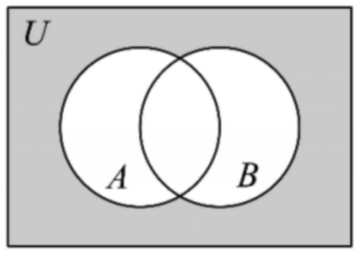
\includegraphics[width=0.20\textwidth]{figures/gao84_q9_venn.png}
\end{center}

\ifanswer
\solbegin
\step{$U=\{1,2,3,4,5,6,7,8,9,10\}$，$A=\{1,2\}$，$B=\{2,4\}$.}
\step{图中阴影部分表示的集合为 $\overline{A\cup B}=\{3,5,6,7,8,9,10\}$，共 $7$ 个元素，}
\step{其非空真子集的个数为 $2^7-2=126$.}
\solend
\fi

\item 若不等式 $ax^2-5x+c<0$ 的解集是 $(2,3)$，则不等式 $cx^2+5x+a\geqslant0$ 的解集是\blankline[4.4em].

\ifanswer
\solbegin
\step{若不等式 $ax^2-5x+c<0$ 的解集是 $(2,3)$，则 $a>0$ 且 $\begin{cases}\dfrac5a=5\\[2pt] \dfrac ca=6\end{cases}$，}
\step{则 $a=1$，$c=6$，}
\step{则不等式 $cx^2+5x+a\geqslant0$ 可化为 $6x^2+5x+1\geqslant0$，则 $x\leqslant-\dfrac12$ 或 $x\geqslant-\dfrac13$，}
\step{则不等式的解集为 $\left(-\infty,-\dfrac12\right]\cup\left[-\dfrac13,+\infty\right)$.}
\solend
\fi

\item 若关于 $x$ 的方程 $mx^2+2x+2=0$ 至少有一个负实根，则实数 $m$ 的取值范围是\blankline[4.4em].

\ifanswer
\solbegin
\step{①当 $m=0$ 时，方程为 $2x+2=0$，有一个负根，满足题意，}
\step{②当 $m\neq0$ 时，关于 $x$ 的方程 $mx^2+2x+2=0$ 至少有一个负根，}
\step{设根为 $x_1$、$x_2$，}
\step{当 $\Delta=4-8m=0$ 时，即 $m=\dfrac12$ 时，方程为 $\dfrac12x^2+2x+1=0$，}
\step{解得 $x=-2$，满足题意，}
\step{当 $\Delta=4-8m>0$，即 $m<\dfrac12$ 时，且 $m\neq0$ 时，}
\step{若有一个负根，则 $x_1x_2=\dfrac2m<0$，解得 $m<0$，}
\step{若有两个负根，则 $\begin{cases}x_1+x_2=-\dfrac2m<0\\[2pt] x_1x_2=\dfrac2m>0\end{cases}$，解得 $0<m<\dfrac12$，}
\step{综上所述，则实数 $m$ 的取值范围是 $\left(-\infty,\dfrac12\right]$.}
\solend
\fi

\item 设集合 $S$、$T$ 都至少含有两个元素，且 $S$、$T$ 同时满足：条件 1：对任意 $x$、$y\in S$，若
$x\neq y$，则 $x+y\in T$；条件 2：对任意 $x$、$y\in T$，若 $x\neq y$，则 $x-y\in S$. 给出下列说法：

①若 $S$ 只有 $2$ 个元素，则这 $2$ 个元素互为相反数；

②若 $S$ 只有 $2$ 个元素，则 $S\cup T$ 必有 $3$ 个元素；

③若 $S$ 只有 $2$ 个元素，则 $S\cup T$ 可能有 $4$ 个元素；

④存在含有 $3$ 个元素的集合 $S$，满足 $S\cup T$ 有 $4$ 个元素.

其中所有正确说法的序号是\blankline[4.4em].

\ifanswer
\solbegin
\step{对于①：由条件 2 得 $x-y\in S$，$y-x\in S$，且 $x-y\neq y-x$，}
\step{所以若 $S$ 只有 $2$ 个元素，则这 $2$ 个元素互为相反数，故①正确；}
\step{对于④：若 $S$ 有 $3$ 个元素，不妨设 $S=\{a,b,c\}$，其中 $a<b<c$，}
\step{则 $\{a+b,b+c,c+a\}\subseteq T$，所以 $c-a$、$c-b$、$b-a$、$a-c$、$b-c$、$a-b\in S$，}
\step{而 $c-a$ 与 $c-b$ 为两个互不相等的正数，$a-c$ 与 $a-b$ 为两个互不相等的负数，}
\step{故集合 $S$ 中至少有 $4$ 个元素，与 $S=\{a,b,c\}$ 有 $3$ 个元素矛盾，故④错误.}
\step{对于②③：若 $S$ 有 $2$ 个元素，由①得集合 $S$ 中的 $2$ 个元素必为相反数，}
\step{故可设 $S=\{a,-a\}(a\neq0)$. 由条件 1 得 $0\in T$，}
\step{由于集合 $T$ 中至少有 $2$ 个元素，故至少还有另外一个元素 $m\in T$.}
\step{当集合 $T$ 只有 $2$ 个元素时即 $T=\{0,m\}$，由条件 1 得 $-m\in S$，则 $m=\pm a$，}
\step{$T=\{0,a\}$ 或 $T=\{0,-a\}$，故 $S\cup T=\{0,a,-a\}$.}
\step{当集合 $T$ 有多于 $2$ 个元素时，不妨设 $T=\{0,m,n\}$，}
\step{则 $m$、$n$、$-m$、$-n$、$m-n$、$n-m\in S$，由于 $m$、$n\neq0$，}
\step{所以 $m\neq m-n$，$n\neq n-m$，又 $m\neq n$，}
\step{故集合 $S$ 至少有 $3$ 个元素，与 $S$ 中只有两个元素矛盾.}
\step{综上，$S\cup T=\{0,a,-a\}$，故②正确，③错误.}
\step{故正确的是①②.}
\solend
\fi

\end{enumerate}

\bigsec{二、选择题}

\begin{enumerate}
\setcounter{enumi}{12}

\item 用反证法证明命题：“若 $x+y>2$，则 $x>1$ 或 $y>1$”时，应假设\mbox{（\quad）}

\keepwithprev
A. $x\leqslant1$ 或 $y\leqslant1$\qquad B. 若 $x>1$ 或 $y>1$

C. $x\leqslant1$ 且 $y\leqslant1$\qquad D. 若 $x>1$ 且 $y>1$

\ifanswer
\ans{$C$}
\fi

\item 下列命题中，为真命题的是\mbox{（\quad）}

\keepwithprev
A. 若 $a>b$，则 $a^2>b^2$\qquad B. 若 $a>b$，$c>d$，则 $ac>bd$

C. 若 $a>b$，则 $\dfrac1a<\dfrac1b$\qquad D. 若 $ac^2>bc^2$，则 $a>b$

\ifanswer
\solbegin
\step{对于 $A$，当 $a=-1$，$b=-2$ 时，$a^2<b^2$，故 $A$ 错误；}
\step{对于 $B$，当 $a=-1$，$b=-2$，$c=-1$，$d=-2$ 时，$ac<bd$，故 $B$ 错误；}
\step{对于 $C$，当 $a=1$，$b=-2$ 时，$\dfrac1a>\dfrac1b$，故 $C$ 错误；}
\step{对于 $D$，因为 $ac^2-bc^2=(a-b)c^2>0$，所以 $a-b>0$，$c^2>0$，则 $a>b$，}
\step{故 $D$ 正确.}
\step{故选 $D$.}
\solend
\fi

\item 现有一级小麦 $m\,\mathrm{kg}$，二级小麦 $n\,\mathrm{kg}$，某粮食收购站有两种收购方案. 方案一：分两个
等级收购小麦，一级小麦 $a$ 元$/\mathrm{kg}$，二级小麦 $b$ 元$/\mathrm{kg}\,(b<a)$；方案二：以方案一两种价
格的平均数收购. 收购方式更加优惠的是\mbox{（\quad）}

\keepwithprev
A. 方案一\qquad B. 方案二\qquad C. 同样优惠\qquad D. 以上均有可能

\ifanswer
\solbegin
\step{方案一收购的平均价格为 $\dfrac{ma+nb}{m+n}$，方案二收购的平均价格为 $\dfrac{a+b}2$；}
\step{所以 $\dfrac{ma+nb}{m+n}-\dfrac{a+b}2=\dfrac{(a-b)(m-n)}{2(m+n)}$ ①，}
\step{$a-b>0$，$m-n$ 的正负性不确定，故①式的正负性不确定，故选 $D$.}
\solend
\fi

\item 用 $C(A)$ 表示非空集合 $A$ 中的元素个数. 对于集合 $A$、$B$，定义

$A*B=\begin{cases}C(A)-C(B),&C(A)\geqslant C(B)\\ C(B)-C(A),&C(A)<C(B)\end{cases}$，若 $A=\{0,1\}$，

$B=\{x\mid(x^2-ax)(x^2+ax+2)=0\}$，设实数 $a$ 的所有可能取值组成的集合是 $S$，则下列选
项不正确的是\mbox{（\quad）}

\keepwithprev
A. $C(B)$ 的可能值为 $1$，$2$，$3$，$4$

B. 若 $A*B=2$，则 $a$ 的取值范围为 $(-\infty,-2\sqrt2)\cup(2\sqrt2,+\infty)$

C. 若 $A*B=1$，则 $C(S)=3$

D. 若 $A*B=0$，则 $a$ 的取值范围为 $(-2\sqrt2,2\sqrt2)$

\ifanswer
\solbegin
\step{对于集合 $B$，当 $a=0$ 时，方程 $x^2(x^2+2)=0$ 的解为 $x=0$，$C(B)=1$，}
\step{当 $a\neq0$ 时，$x^2-ax=0$ 或 $x^2+ax+2=0$，}
\step{其中 $x^2-ax=0$ 的解为 $x_1=0$，$x_2=a$，}
\step{若 $\Delta=a^2-8>0$，即 $a>2\sqrt2$ 或 $a<-2\sqrt2$，}
\step{方程 $x^2+ax+2=0$ 有两个不相等的实数根，此时 $C(B)=4$；}
\step{若 $\Delta=a^2-8=0$，即 $a=2\sqrt2$ 或 $-2\sqrt2$，}
\step{方程 $x^2+ax+2=0$ 有两个相等的实数根，此时 $C(B)=3$；}
\step{若 $\Delta=a^2-8<0$，即 $-2\sqrt2<a<0$ 或 $0<a<2\sqrt2$，}
\step{方程 $x^2+ax+2=0$ 无实数根，此时 $C(B)=2$；}
\step{所以 $C(B)$ 的可能值为 $1$，$2$，$3$，$4$，故 $A$ 正确；}
\step{若 $A*B=2$，且 $C(A)=2$，则 $C(B)=4$，}
\step{则 $a$ 的取值范围 $(-\infty,-2\sqrt2)\cup(2\sqrt2,+\infty)$，故 $B$ 正确；}
\step{若 $A*B=1$，且 $C(A)=2$，则 $C(B)=1$ 或 $3$，}
\step{当 $C(B)=1$ 时，$a=0$，}
\step{当 $C(B)=3$ 时，$a=2\sqrt2$ 或 $-2\sqrt2$，此时集合 $S=\{0,-2\sqrt2,2\sqrt2\}$，}
\step{则 $C(S)=3$，故 $C$ 正确；}
\step{若 $A*B=0$，且 $C(A)=2$，则 $C(B)=2$，}
\step{由此可得 $a$ 的取值范围为 $(-2\sqrt2,0)\cup(0,2\sqrt2)$，故 $D$ 不正确；}
\step{故选 $D$.}
\solend
\fi

\end{enumerate}

\bigsec{三、解答题}

\begin{enumerate}
\setcounter{enumi}{16}

\item 已知集合 $A=\{x\mid-3<x\leqslant4\}$，集合 $B=\{x\mid k+1\leqslant x\leqslant2k-1\}$.

（1）当 $k=3$ 时，求 $A\cup B$、$\overline A\cap B$；

（2）若 $B\subseteq A$，求 $k$ 的取值范围.

\ansspace*[10]

\ifanswer
\solbegin
\stepm{（1）}{当 $k=3$ 时，$B=\{x\mid4\leqslant x\leqslant5\}$，又 $A=\{x\mid-3<x\leqslant4\}$，}
\step{所以 $\overline A=\{x\mid x\leqslant-3$ 或 $x>4\}$，}
\step{所以 $A\cup B=\{x\mid-3<x\leqslant5\}$，$\overline A\cap B=\{x\mid4<x\leqslant5\}$.}
\stepm{（2）}{①当 $B=\varnothing$，即 $k+1>2k-1$ 时，$k<2$，满足 $B\subseteq A$.}
\step{②当 $B\neq\varnothing$ 时，由 $B\subseteq A$ 得 $\begin{cases}k+1\leqslant2k-1\\ k+1>-3\\ 2k-1\leqslant4\end{cases}$，解得 $2\leqslant k\leqslant\dfrac52$，}
\step{综合①②得 $k$ 的取值范围 $\left\{k\mid k\leqslant\dfrac52\right\}$.}
\solend
\fi

\item 设集合 $A=\{x\mid x^2-3x+2=0\}$，$B=\{x\mid x^2+2(a+1)x+a^2-5=0\}$.

（1）若 $A\cap B=\{2\}$，求实数 $a$ 的值；

（2）若集合 $B$ 中有两个元素 $x_1,x_2$，求 $\lvert x_1-x_2\rvert$（用 $a$ 表示）.

\ansspace*[10]

\ifanswer
\solbegin
\stepm{（1）}{由题意得 $A=\{x\mid x^2-3x+2=0\}=\{1,2\}$，因为 $A\cap B=\{2\}$，所以 $2\in B$，}
\step{所以 $2^2+4(a+1)+a^2-5=0$ 即 $4+4a+4+a^2-5=0$，}
\step{化简得 $a^2+4a+3=0$，即 $(a+3)(a+1)=0$，解得 $a=-3$ 或 $a=-1$，}
\step{检验：当 $a=-3$ 时，$B=\{x\mid x^2-4x+4=0\}=\{2\}$，满足 $A\cap B=\{2\}$，}
\step{当 $a=-1$ 时，$B=\{x\mid x^2-4=0\}=\{-2,2\}$，满足 $A\cap B=\{2\}$，}
\step{所以 $a=-3$ 或 $a=-1$.}
\stepm{（2）}{因为 $B$ 中有两个元素 $x_1,x_2$，所以 $x^2+2(a+1)x+(a^2-5)=0$ 有两个根，}
\step{所以 $\Delta=4(a+1)^2-4(a^2-5)=8a+24>0$，}
\step{且 $x_1+x_2=-2(a+1)$，$x_1x_2=a^2-5$，}
\step{所以 $\lvert x_1-x_2\rvert=\sqrt{(x_1+x_2)^2-4x_1x_2}=\sqrt{4(a+1)^2-4(a^2-5)}=\sqrt{8a+24}$.}
\solend
\fi

\item 已知关于 $x$ 的不等式 $\dfrac{ax-2}{1+x}>0$.

（1）若 $x=-a$ 时，不等式成立，求实数 $a$ 的取值范围；

（2）若 $a$ 为实数，解关于 $x$ 的不等式：$\dfrac{ax-2}{1+x}>0$.

\ansspace*[12]

\ifanswer
\solbegin
\stepm{（1）}{因为 $x=-a$ 时，不等式成立，}
\step{所以 $\dfrac{-a^2-2}{1-a}>0\Rightarrow\dfrac{a^2+2}{a-1}>0\Rightarrow a-1>0\Rightarrow a>1$，}
\step{所以实数 $a$ 的取值范围为 $(1,+\infty)$.}
\stepm{（2）}{$\dfrac{ax-2}{1+x}>0\Rightarrow(ax-2)(x+1)>0$，}
\step{当 $a=0$ 时，$-2(x+1)>0$，解得 $x<-1$.}
\step{当 $a>0$ 时，$(ax-2)(x+1)>0$，解得 $x>\dfrac2a$ 或 $x<-1$.}
\step{当 $a<0$ 时，不等式 $(ax-2)(x+1)>0$ 可化为 $\left(x-\dfrac2a\right)(x+1)<0$，}
\step{当 $\dfrac2a>-1$，即 $a<-2$ 时，解得 $-1<x<\dfrac2a$；}
\step{当 $\dfrac2a<-1$，即 $-2<a<0$ 时，解得 $\dfrac2a<x<-1$；}
\step{当 $\dfrac2a=-1$，即 $a=-2$ 时，解集为 $\varnothing$.}
\step{综上，当 $a<-2$ 时，不等式的解集为 $\left(-1,\dfrac2a\right)$；}
\step{当 $a=-2$ 时，不等式的解集为 $\varnothing$；}
\step{当 $-2<a<0$ 时，不等式的解集为 $\left(\dfrac2a,-1\right)$；}
\step{当 $a=0$ 时，不等式的解集为 $(-\infty,-1)$；}
\step{当 $a>0$ 时，不等式的解集为 $(-\infty,-1)\cup\left(\dfrac2a,+\infty\right)$.}
\solend
\fi

\item 已知关于 $x$ 的不等式 $(k^2-2k-3)x^2+(k+1)x+1>0\,(k\in\R)$ 的解集为 $M$；

（1）若存在实数 $a$，使得 $M=(-\infty,a)\cup(a,+\infty)$，求 $k$ 的值；

（2）若 $M=\R$，求 $k$ 的取值范围；

（3）是否存在实数 $k$，满足：“对于任意 $n\in\N$，$n>0$，都有 $n\in M$；对于任意
$m\in\Z$，$m<0$，都有 $m\notin M$”，若存在，求出 $k$ 的值，若不存在，说明理由.

\ansspace*[13]

\ifanswer
\solbegin
\stepm{（1）}{记 $f(x)=(k^2-2k-3)x^2+(k+1)x+1$.}
\step{$M=(-\infty,a)\cup(a,+\infty)$ 表示 $f(x)>0$ 对一切 $x\neq a$ 成立，且 $f(a)=0$，}
\step{故需二次项系数大于 $0$ 且 $\Delta=0$.}
\step{由 $\Delta=(k+1)^2-4(k^2-2k-3)=-3k^2+10k+13=0$ 得 $k=\dfrac{13}3$ 或 $k=-1$.}
\step{当 $k=\dfrac{13}3$ 时，二次项系数 $\dfrac{64}9>0$，$f(x)=\dfrac{64}9\left(x+\dfrac38\right)^2$，符合；}
\step{当 $k=-1$ 时二次项系数为 $0$，$f(x)=1>0$，$M=\R$，不符合. 故 $k=\dfrac{13}3$.}
\stepm{（2）}{$M=\R$ 即 $f(x)>0$ 对一切 $x\in\R$ 恒成立.}
\step{①当 $k^2-2k-3>0$（即 $k<-1$ 或 $k>3$）时，需 $\Delta<0$，}
\step{即 $-3k^2+10k+13<0$，得 $k<-1$ 或 $k>\dfrac{13}3$，故 $k<-1$ 或 $k>\dfrac{13}3$；}
\step{②当 $k^2-2k-3=0$ 时，$k=3$ 得 $f(x)=4x+1$ 不恒正，不符合题意，}
\step{舍去，}
\step{当 $k=-1$ 得 $f(x)=1>0$ 恒成立，符合题意；}
\step{③当 $k^2-2k-3<0$ 时，抛物线开口向下，不能恒正.}
\step{综上，$k\leqslant-1$ 或 $k>\dfrac{13}3$.}
\stepm{（3）}{存在，$k=3$，理由如下，}
\step{由题意得解集 $M=(t,+\infty)$，$t\in[-1,1)$；}
\step{当 $k^2-2k-3=0$ 时，解得 $k=3$ 或 $k=-1$，}
\step{$k=3$ 时，不等式的解集为 $\left(-\dfrac14,+\infty\right)$，满足条件；}
\step{$k=-1$ 时，$1>0$ 恒成立，不满足条件；}
\step{当 $k^2-2k-3>0$ 时，}
\step{此时对应的一元二次不等式的解集形式不是 $(t,+\infty)$ 的形式，不满足条件；}
\step{当 $k^2-2k-3<0$ 时，}
\step{此时对应的一元二次不等式的解集形式不是 $(t,+\infty)$ 的形式，不满足条件；}
\step{综上，满足条件 $k$ 的值为 $3$.}
\solend
\fi

\item 已知有限集 $A=\{a_1,a_2,\cdots,a_n\}\,(n\geqslant2,n\in\N)$，如果 $A$ 中元素 $a_i\,(i=1,2,3,\cdots,n)$ 满足
$a_1+a_2+a_3+\cdots+a_n=a_1\times a_2\times\cdots\times a_n$，就称 $A$ 为“和积平衡集”.

（1）判断集合 $\{-1+\sqrt3,-1-\sqrt3\}$ 是否为“和积平衡集”；

（2）若 $a_1$、$a_2$ 是两个不同的正数，且 $\{a_1,a_2\}$ 是“和积平衡集”，写出以 $a_1$、$a_2$ 为根的一
个一元二次方程（系数可用 $a_1$、$a_2$ 表示），并证明 $a_1$、$a_2$ 至少有一个大于 $2$；

（3）若 $a_i\in\Z$ 且 $a_i>0$，求所有符合条件的“和积平衡集”.

\ansspace*[14]

\ifanswer
\solbegin
\stepm{（1）}{对于集合 $\{-1+\sqrt3,-1-\sqrt3\}$，}
\step{因为 $(-1+\sqrt3)+(-1-\sqrt3)=-2$，$(-1+\sqrt3)\times(-1-\sqrt3)=-2$，}
\step{所以满足 $a_1+a_2=a_1\times a_2$，满足题意，}
\step{所以集合 $\{-1+\sqrt3,-1-\sqrt3\}$ 是和积平衡集.}
\stepm{（2）}{以 $a_1$、$a_2$ 为根的一个一元二次方程可为 $x^2-(a_1+a_2)x+a_1\cdot a_2=0$，}
\step{因为 $a_1$、$a_2$ 是两个不同的正数，且 $\{a_1,a_2\}$ 是和积平衡集，}
\step{所以 $a_1+a_2=a_1\cdot a_2$，}
\step{又 $a_1$ 和 $a_2$ 为 $x^2-(a_1+a_2)x+a_1\cdot a_2=0$ 的两个不同的正根，}
\step{所以 $\Delta=(a_1+a_2)^2-4a_1a_2=(a_1+a_2)^2-4(a_1+a_2)>0$，}
\step{又 $a_1+a_2>0$，则 $a_1+a_2>4$，}
\step{若 $a_1$、$a_2$ 都小于等于 $2$，则 $a_1+a_2\leqslant4$，矛盾，}
\step{所以 $a_1$、$a_2$ 至少有一个大于 $2$；}
\stepm{（3）}{设 $A$ 中的 $a_1<a_2<a_3<\cdots<a_n$，且 $a_i\in\N^*$，}
\step{由 $a_1+a_2+a_3+\cdots+a_n=a_1\times a_2\times\cdots\times a_n$，得 $n=2$ 时明显不满足，}
\step{所以 $n\geqslant3$，故 $a_1\times a_2\times\cdots\times a_n=a_1+a_2+a_3+\cdots+a_n\leqslant na_n$，}
\step{所以 $a_1\times a_2\times\cdots\times a_{n-1}\leqslant n$，}
\step{当 $n=3$ 时，$a_1\times a_2\leqslant3$，$a_i\in\N^*$，只能有 $a_1=1$，$a_2=2$，}
\step{由 $a_1+a_2+a_3=a_1\times a_2\times a_3$，得 $a_3=3$，此时的和积平衡集为 $\{1,2,3\}$，}
\step{当 $n\geqslant4$ 时，$a_1\times a_2\times\cdots\times a_{n-1}\geqslant(n-1)(n-2)\times\cdots\times2\times1\geqslant(n-1)(n-2)$，}
\step{又 $(n-1)(n-2)-n=n^2-4n+2=n(n-4)+2>0$，即 $(n-1)(n-2)>n$，}
\step{即 $a_1\times a_2\times\cdots\times a_{n-1}>n$，与 $a_1\times a_2\times\cdots\times a_{n-1}\leqslant n$ 矛盾，}
\step{所以 $n\geqslant4$ 不满足条件，}
\step{所以符合条件的和积平衡集有且只有 $n=3$，此时的和积平衡集为 $\{1,2,3\}$.}
\solend
\fi

\end{enumerate}

\end{document}
"
% 紧凑版：xelatex "\def\iscompact{1}% 高一84_东昌中学_10月月考.tex
%   —— 高一上数学“2026-2027 年东昌中学高一上 10 月月考”（讲评版）
% 试卷版：xelatex 高一84_东昌中学_10月月考.tex
% 答案版：xelatex "\def\isanswer{1}% 高一84_东昌中学_10月月考.tex
%   —— 高一上数学“2026-2027 年东昌中学高一上 10 月月考”（讲评版）
% 试卷版：xelatex 高一84_东昌中学_10月月考.tex
% 答案版：xelatex "\def\isanswer{1}\input{高一84_东昌中学_10月月考.tex}"
% 紧凑版：xelatex "\def\iscompact{1}\input{高一84_东昌中学_10月月考.tex}"
%
% 原始材料：微信公众号“魔都数学加油站”文章，连载“27学年高一84”；
% 原文标题“27学年高一84——2026-2027年上海市东昌中学高一上10月月考”；
% 原文链接：https://mp.weixin.qq.com/s/PErsjO3N5RsMuJC69IGbrw。
% 页面标注发布时间 2026-10-26 20:15（上海）。
% 正文为 12 张 PNG 页（`原图/高一84_东昌中学_10月月考/01..12.png`），
% 尺寸混排（第 1—8 页为 4762×6735，第 9—12 页为 2560×3620），均按页序读取。
%
% 篇幅与题号：原卷自第 3 题起编号（第 1、2 题不在原文内）。填空题 3—12（10 题）、
% 选择题 13—16（4 题）、解答题 17—21（5 题），共 19 题。
%
% 讲评版：19 题全部印【解析】，本稿不另提 \ans{}；选择题答案在解析末句“故选 D／C／D”。
% 第 13 题的答案“C”原卷直接印在题干括号内（“（\ C\ ）”），本稿按 高一37 第 13 题／
% 高一63 第 14 题成例括号留空、另提 \ans{$C$}（该题无【解析】段）。
%
% 副标题：原卷未印副标题。本稿按内容标作“集合与常用逻辑用语、不等式”。
%
% 与原卷的排版差异：
%   ① 原卷每题下直接印【解析】，本稿按全稿惯例将解析置于答案版；
%   ② 原卷未印副标题，本稿补出；填空横线统一排 \blankline[4.4em]；
%   ③ 原卷数集记号排斜体 $R$、$Z$、$N$，本稿按全稿惯例改用 $\R$、$\Z$、$\N$；
%   ④ 第 17—21 题的子问用行内“（1）（2）（3）”段，解析中的子问标号用 \stepm；
%   ⑤ 解答题按惯例加 \ansspace；选择题括号排 \mbox{（\quad）}；
%   ⑥ 第 9 题题干右侧有一幅韦恩图，裁自原图（第 2 页）后去粉色水印、转灰度，
%      三版都出（属题干）。
%
% 行数核对：逐题数 \step/\stepm 条数，合计 157 条（Q3：2；Q4：2；Q5：3；Q6：2；
% Q7：3；Q8：6；Q9：3；Q10：4；Q11：9；Q12：17；Q14：6；Q15：3；Q16：19；
% Q17：6；Q18：10；Q19：15；Q20：24；Q21：23）；第 13 题无解析，只提 \ans{}，
% 不计入 \step 账。原卷解析的换行按语意合并，未逐行强拆。
%
\documentclass[a4paper,11pt]{article}
\usepackage{common}

\begin{document}

\examtitlest[4]{2026--2027 年东昌中学高一上 10 月月考}{集合与常用逻辑用语、不等式}

\bigsec{一、填空题}

\begin{enumerate}
\setcounter{enumi}{2}

\item 若 $a\in\R$，则“$a=2$”是“$(a-1)(a-2)=0$”的\blankline[3.6em]条件（填“充分不必要”、“必要
不充分”、“充要”、“既不充分又不必要”的一个）.

\ifanswer
\solbegin
\step{$a=2\Rightarrow(a-1)(a-2)=0$，而 $(a-1)(a-2)=0$ 不能推出 $a=2$，}
\step{故“$a=2$”是“$(a-1)(a-2)=0$”的充分不必要条件.}
\solend
\fi

\item 已知集合 $M=\{(x,y)\mid y=x^2\}$，$N=\{(x,y)\mid y=1\}$，则 $M\cap N=\blankline[4.4em]$.

\ifanswer
\solbegin
\step{集合 $M=\{(x,y)\mid y=x^2\}$，$N=\{(x,y)\mid y=1\}$，}
\step{当 $y=1$ 时，$x=\pm1$，则 $M\cap N=\{(-1,1),(1,1)\}$.}
\solend
\fi

\item 已知集合 $A=\{x\mid x^2+ax+4=0\}$，若 $A$ 有且只有一个非空子集，则实数 $a=\blankline[4.4em]$.

\ifanswer
\solbegin
\step{因为集合 $A$ 有且只有一个非空子集，所以集合 $A$ 中只有一个元素，}
\step{所以一元二次方程 $x^2+ax+4=0$ 有两个相等的解，}
\step{所以 $\Delta=a^2-4\times4=0$，解得 $a=\pm4$.}
\solend
\fi

\item 已知 $A=(-\infty,a]$，$B=(-\infty,3)$，且 $x\in A$ 是 $x\in B$ 的充分不必要条件，则 $a$ 的取值范围
是\blankline[4.4em].

\ifanswer
\solbegin
\step{$A=(-\infty,a]$，$B=(-\infty,3)$，且 $x\in A$ 是 $x\in B$ 的充分不必要条件，}
\step{则 $A\subset B$，则 $a<3$，即 $a$ 的取值范围为 $(-\infty,3)$.}
\solend
\fi

\item 不等式 $\dfrac{3x-1}{x-2}\leqslant1$ 的解集为\blankline[4.4em].

\ifanswer
\solbegin
\step{由 $\dfrac{3x-1}{x-2}\leqslant1$，得 $\dfrac{3x-1}{x-2}-1=\dfrac{3x-1-(x-2)}{x-2}=\dfrac{2x+1}{x-2}\leqslant0$，}
\step{则 $\begin{cases}(2x+1)(x-2)\leqslant0\\ x-2\neq0\end{cases}$，解得 $-\dfrac12\leqslant x<2$，}
\step{则不等式 $\dfrac{3x-1}{x-2}\leqslant1$ 的解集为 $\left[-\dfrac12,2\right)$.}
\solend
\fi

\item 已知关于 $x$ 的一元二次方程 $x^2-2mx+(3m+1)=0$ 的两个实数根为 $x_1$、$x_2$，且
$x_1^2+x_2^2=16$，则实数 $m$ 的值为\blankline[4.4em].

\ifanswer
\solbegin
\step{由韦达定理，得 $x_1+x_2=2m$，$x_1x_2=3m+1$，}
\step{$x_1^2+x_2^2=(x_1+x_2)^2-2x_1x_2=4m^2-6m-2$，}
\step{由 $x_1^2+x_2^2=16$，得 $4m^2-6m-2=16$，即 $2m^2-3m-9=0$，}
\step{解得 $m=3$ 或 $m=-\dfrac32$，}
\step{检验判别式 $\Delta=4m^2-12m-4$，当 $m=3$ 时，$\Delta=-4<0$，舍去；}
\step{当 $m=-\dfrac32$ 时，$\Delta=23>0$，符合条件，故 $m=-\dfrac32$.}
\solend
\fi

\item 已知全集 $U=\{x\mid1\leqslant x\leqslant10,\,x\in\N\}$，集合 $A=\{x\mid x^2-3<4,\,x\in\N,\,x>0\}$，
$B=\{2,4\}$，则图中阴影部分表示的集合的非空真子集个数为\blankline[4.4em].

\needvspace{9\baselineskip}
\begin{center}
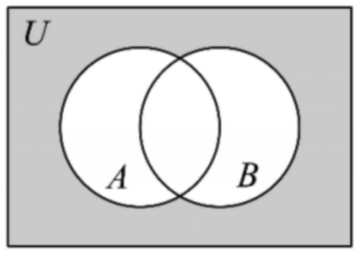
\includegraphics[width=0.20\textwidth]{figures/gao84_q9_venn.png}
\end{center}

\ifanswer
\solbegin
\step{$U=\{1,2,3,4,5,6,7,8,9,10\}$，$A=\{1,2\}$，$B=\{2,4\}$.}
\step{图中阴影部分表示的集合为 $\overline{A\cup B}=\{3,5,6,7,8,9,10\}$，共 $7$ 个元素，}
\step{其非空真子集的个数为 $2^7-2=126$.}
\solend
\fi

\item 若不等式 $ax^2-5x+c<0$ 的解集是 $(2,3)$，则不等式 $cx^2+5x+a\geqslant0$ 的解集是\blankline[4.4em].

\ifanswer
\solbegin
\step{若不等式 $ax^2-5x+c<0$ 的解集是 $(2,3)$，则 $a>0$ 且 $\begin{cases}\dfrac5a=5\\[2pt] \dfrac ca=6\end{cases}$，}
\step{则 $a=1$，$c=6$，}
\step{则不等式 $cx^2+5x+a\geqslant0$ 可化为 $6x^2+5x+1\geqslant0$，则 $x\leqslant-\dfrac12$ 或 $x\geqslant-\dfrac13$，}
\step{则不等式的解集为 $\left(-\infty,-\dfrac12\right]\cup\left[-\dfrac13,+\infty\right)$.}
\solend
\fi

\item 若关于 $x$ 的方程 $mx^2+2x+2=0$ 至少有一个负实根，则实数 $m$ 的取值范围是\blankline[4.4em].

\ifanswer
\solbegin
\step{①当 $m=0$ 时，方程为 $2x+2=0$，有一个负根，满足题意，}
\step{②当 $m\neq0$ 时，关于 $x$ 的方程 $mx^2+2x+2=0$ 至少有一个负根，}
\step{设根为 $x_1$、$x_2$，}
\step{当 $\Delta=4-8m=0$ 时，即 $m=\dfrac12$ 时，方程为 $\dfrac12x^2+2x+1=0$，}
\step{解得 $x=-2$，满足题意，}
\step{当 $\Delta=4-8m>0$，即 $m<\dfrac12$ 时，且 $m\neq0$ 时，}
\step{若有一个负根，则 $x_1x_2=\dfrac2m<0$，解得 $m<0$，}
\step{若有两个负根，则 $\begin{cases}x_1+x_2=-\dfrac2m<0\\[2pt] x_1x_2=\dfrac2m>0\end{cases}$，解得 $0<m<\dfrac12$，}
\step{综上所述，则实数 $m$ 的取值范围是 $\left(-\infty,\dfrac12\right]$.}
\solend
\fi

\item 设集合 $S$、$T$ 都至少含有两个元素，且 $S$、$T$ 同时满足：条件 1：对任意 $x$、$y\in S$，若
$x\neq y$，则 $x+y\in T$；条件 2：对任意 $x$、$y\in T$，若 $x\neq y$，则 $x-y\in S$. 给出下列说法：

①若 $S$ 只有 $2$ 个元素，则这 $2$ 个元素互为相反数；

②若 $S$ 只有 $2$ 个元素，则 $S\cup T$ 必有 $3$ 个元素；

③若 $S$ 只有 $2$ 个元素，则 $S\cup T$ 可能有 $4$ 个元素；

④存在含有 $3$ 个元素的集合 $S$，满足 $S\cup T$ 有 $4$ 个元素.

其中所有正确说法的序号是\blankline[4.4em].

\ifanswer
\solbegin
\step{对于①：由条件 2 得 $x-y\in S$，$y-x\in S$，且 $x-y\neq y-x$，}
\step{所以若 $S$ 只有 $2$ 个元素，则这 $2$ 个元素互为相反数，故①正确；}
\step{对于④：若 $S$ 有 $3$ 个元素，不妨设 $S=\{a,b,c\}$，其中 $a<b<c$，}
\step{则 $\{a+b,b+c,c+a\}\subseteq T$，所以 $c-a$、$c-b$、$b-a$、$a-c$、$b-c$、$a-b\in S$，}
\step{而 $c-a$ 与 $c-b$ 为两个互不相等的正数，$a-c$ 与 $a-b$ 为两个互不相等的负数，}
\step{故集合 $S$ 中至少有 $4$ 个元素，与 $S=\{a,b,c\}$ 有 $3$ 个元素矛盾，故④错误.}
\step{对于②③：若 $S$ 有 $2$ 个元素，由①得集合 $S$ 中的 $2$ 个元素必为相反数，}
\step{故可设 $S=\{a,-a\}(a\neq0)$. 由条件 1 得 $0\in T$，}
\step{由于集合 $T$ 中至少有 $2$ 个元素，故至少还有另外一个元素 $m\in T$.}
\step{当集合 $T$ 只有 $2$ 个元素时即 $T=\{0,m\}$，由条件 1 得 $-m\in S$，则 $m=\pm a$，}
\step{$T=\{0,a\}$ 或 $T=\{0,-a\}$，故 $S\cup T=\{0,a,-a\}$.}
\step{当集合 $T$ 有多于 $2$ 个元素时，不妨设 $T=\{0,m,n\}$，}
\step{则 $m$、$n$、$-m$、$-n$、$m-n$、$n-m\in S$，由于 $m$、$n\neq0$，}
\step{所以 $m\neq m-n$，$n\neq n-m$，又 $m\neq n$，}
\step{故集合 $S$ 至少有 $3$ 个元素，与 $S$ 中只有两个元素矛盾.}
\step{综上，$S\cup T=\{0,a,-a\}$，故②正确，③错误.}
\step{故正确的是①②.}
\solend
\fi

\end{enumerate}

\bigsec{二、选择题}

\begin{enumerate}
\setcounter{enumi}{12}

\item 用反证法证明命题：“若 $x+y>2$，则 $x>1$ 或 $y>1$”时，应假设\mbox{（\quad）}

\keepwithprev
A. $x\leqslant1$ 或 $y\leqslant1$\qquad B. 若 $x>1$ 或 $y>1$

C. $x\leqslant1$ 且 $y\leqslant1$\qquad D. 若 $x>1$ 且 $y>1$

\ifanswer
\ans{$C$}
\fi

\item 下列命题中，为真命题的是\mbox{（\quad）}

\keepwithprev
A. 若 $a>b$，则 $a^2>b^2$\qquad B. 若 $a>b$，$c>d$，则 $ac>bd$

C. 若 $a>b$，则 $\dfrac1a<\dfrac1b$\qquad D. 若 $ac^2>bc^2$，则 $a>b$

\ifanswer
\solbegin
\step{对于 $A$，当 $a=-1$，$b=-2$ 时，$a^2<b^2$，故 $A$ 错误；}
\step{对于 $B$，当 $a=-1$，$b=-2$，$c=-1$，$d=-2$ 时，$ac<bd$，故 $B$ 错误；}
\step{对于 $C$，当 $a=1$，$b=-2$ 时，$\dfrac1a>\dfrac1b$，故 $C$ 错误；}
\step{对于 $D$，因为 $ac^2-bc^2=(a-b)c^2>0$，所以 $a-b>0$，$c^2>0$，则 $a>b$，}
\step{故 $D$ 正确.}
\step{故选 $D$.}
\solend
\fi

\item 现有一级小麦 $m\,\mathrm{kg}$，二级小麦 $n\,\mathrm{kg}$，某粮食收购站有两种收购方案. 方案一：分两个
等级收购小麦，一级小麦 $a$ 元$/\mathrm{kg}$，二级小麦 $b$ 元$/\mathrm{kg}\,(b<a)$；方案二：以方案一两种价
格的平均数收购. 收购方式更加优惠的是\mbox{（\quad）}

\keepwithprev
A. 方案一\qquad B. 方案二\qquad C. 同样优惠\qquad D. 以上均有可能

\ifanswer
\solbegin
\step{方案一收购的平均价格为 $\dfrac{ma+nb}{m+n}$，方案二收购的平均价格为 $\dfrac{a+b}2$；}
\step{所以 $\dfrac{ma+nb}{m+n}-\dfrac{a+b}2=\dfrac{(a-b)(m-n)}{2(m+n)}$ ①，}
\step{$a-b>0$，$m-n$ 的正负性不确定，故①式的正负性不确定，故选 $D$.}
\solend
\fi

\item 用 $C(A)$ 表示非空集合 $A$ 中的元素个数. 对于集合 $A$、$B$，定义

$A*B=\begin{cases}C(A)-C(B),&C(A)\geqslant C(B)\\ C(B)-C(A),&C(A)<C(B)\end{cases}$，若 $A=\{0,1\}$，

$B=\{x\mid(x^2-ax)(x^2+ax+2)=0\}$，设实数 $a$ 的所有可能取值组成的集合是 $S$，则下列选
项不正确的是\mbox{（\quad）}

\keepwithprev
A. $C(B)$ 的可能值为 $1$，$2$，$3$，$4$

B. 若 $A*B=2$，则 $a$ 的取值范围为 $(-\infty,-2\sqrt2)\cup(2\sqrt2,+\infty)$

C. 若 $A*B=1$，则 $C(S)=3$

D. 若 $A*B=0$，则 $a$ 的取值范围为 $(-2\sqrt2,2\sqrt2)$

\ifanswer
\solbegin
\step{对于集合 $B$，当 $a=0$ 时，方程 $x^2(x^2+2)=0$ 的解为 $x=0$，$C(B)=1$，}
\step{当 $a\neq0$ 时，$x^2-ax=0$ 或 $x^2+ax+2=0$，}
\step{其中 $x^2-ax=0$ 的解为 $x_1=0$，$x_2=a$，}
\step{若 $\Delta=a^2-8>0$，即 $a>2\sqrt2$ 或 $a<-2\sqrt2$，}
\step{方程 $x^2+ax+2=0$ 有两个不相等的实数根，此时 $C(B)=4$；}
\step{若 $\Delta=a^2-8=0$，即 $a=2\sqrt2$ 或 $-2\sqrt2$，}
\step{方程 $x^2+ax+2=0$ 有两个相等的实数根，此时 $C(B)=3$；}
\step{若 $\Delta=a^2-8<0$，即 $-2\sqrt2<a<0$ 或 $0<a<2\sqrt2$，}
\step{方程 $x^2+ax+2=0$ 无实数根，此时 $C(B)=2$；}
\step{所以 $C(B)$ 的可能值为 $1$，$2$，$3$，$4$，故 $A$ 正确；}
\step{若 $A*B=2$，且 $C(A)=2$，则 $C(B)=4$，}
\step{则 $a$ 的取值范围 $(-\infty,-2\sqrt2)\cup(2\sqrt2,+\infty)$，故 $B$ 正确；}
\step{若 $A*B=1$，且 $C(A)=2$，则 $C(B)=1$ 或 $3$，}
\step{当 $C(B)=1$ 时，$a=0$，}
\step{当 $C(B)=3$ 时，$a=2\sqrt2$ 或 $-2\sqrt2$，此时集合 $S=\{0,-2\sqrt2,2\sqrt2\}$，}
\step{则 $C(S)=3$，故 $C$ 正确；}
\step{若 $A*B=0$，且 $C(A)=2$，则 $C(B)=2$，}
\step{由此可得 $a$ 的取值范围为 $(-2\sqrt2,0)\cup(0,2\sqrt2)$，故 $D$ 不正确；}
\step{故选 $D$.}
\solend
\fi

\end{enumerate}

\bigsec{三、解答题}

\begin{enumerate}
\setcounter{enumi}{16}

\item 已知集合 $A=\{x\mid-3<x\leqslant4\}$，集合 $B=\{x\mid k+1\leqslant x\leqslant2k-1\}$.

（1）当 $k=3$ 时，求 $A\cup B$、$\overline A\cap B$；

（2）若 $B\subseteq A$，求 $k$ 的取值范围.

\ansspace*[10]

\ifanswer
\solbegin
\stepm{（1）}{当 $k=3$ 时，$B=\{x\mid4\leqslant x\leqslant5\}$，又 $A=\{x\mid-3<x\leqslant4\}$，}
\step{所以 $\overline A=\{x\mid x\leqslant-3$ 或 $x>4\}$，}
\step{所以 $A\cup B=\{x\mid-3<x\leqslant5\}$，$\overline A\cap B=\{x\mid4<x\leqslant5\}$.}
\stepm{（2）}{①当 $B=\varnothing$，即 $k+1>2k-1$ 时，$k<2$，满足 $B\subseteq A$.}
\step{②当 $B\neq\varnothing$ 时，由 $B\subseteq A$ 得 $\begin{cases}k+1\leqslant2k-1\\ k+1>-3\\ 2k-1\leqslant4\end{cases}$，解得 $2\leqslant k\leqslant\dfrac52$，}
\step{综合①②得 $k$ 的取值范围 $\left\{k\mid k\leqslant\dfrac52\right\}$.}
\solend
\fi

\item 设集合 $A=\{x\mid x^2-3x+2=0\}$，$B=\{x\mid x^2+2(a+1)x+a^2-5=0\}$.

（1）若 $A\cap B=\{2\}$，求实数 $a$ 的值；

（2）若集合 $B$ 中有两个元素 $x_1,x_2$，求 $\lvert x_1-x_2\rvert$（用 $a$ 表示）.

\ansspace*[10]

\ifanswer
\solbegin
\stepm{（1）}{由题意得 $A=\{x\mid x^2-3x+2=0\}=\{1,2\}$，因为 $A\cap B=\{2\}$，所以 $2\in B$，}
\step{所以 $2^2+4(a+1)+a^2-5=0$ 即 $4+4a+4+a^2-5=0$，}
\step{化简得 $a^2+4a+3=0$，即 $(a+3)(a+1)=0$，解得 $a=-3$ 或 $a=-1$，}
\step{检验：当 $a=-3$ 时，$B=\{x\mid x^2-4x+4=0\}=\{2\}$，满足 $A\cap B=\{2\}$，}
\step{当 $a=-1$ 时，$B=\{x\mid x^2-4=0\}=\{-2,2\}$，满足 $A\cap B=\{2\}$，}
\step{所以 $a=-3$ 或 $a=-1$.}
\stepm{（2）}{因为 $B$ 中有两个元素 $x_1,x_2$，所以 $x^2+2(a+1)x+(a^2-5)=0$ 有两个根，}
\step{所以 $\Delta=4(a+1)^2-4(a^2-5)=8a+24>0$，}
\step{且 $x_1+x_2=-2(a+1)$，$x_1x_2=a^2-5$，}
\step{所以 $\lvert x_1-x_2\rvert=\sqrt{(x_1+x_2)^2-4x_1x_2}=\sqrt{4(a+1)^2-4(a^2-5)}=\sqrt{8a+24}$.}
\solend
\fi

\item 已知关于 $x$ 的不等式 $\dfrac{ax-2}{1+x}>0$.

（1）若 $x=-a$ 时，不等式成立，求实数 $a$ 的取值范围；

（2）若 $a$ 为实数，解关于 $x$ 的不等式：$\dfrac{ax-2}{1+x}>0$.

\ansspace*[12]

\ifanswer
\solbegin
\stepm{（1）}{因为 $x=-a$ 时，不等式成立，}
\step{所以 $\dfrac{-a^2-2}{1-a}>0\Rightarrow\dfrac{a^2+2}{a-1}>0\Rightarrow a-1>0\Rightarrow a>1$，}
\step{所以实数 $a$ 的取值范围为 $(1,+\infty)$.}
\stepm{（2）}{$\dfrac{ax-2}{1+x}>0\Rightarrow(ax-2)(x+1)>0$，}
\step{当 $a=0$ 时，$-2(x+1)>0$，解得 $x<-1$.}
\step{当 $a>0$ 时，$(ax-2)(x+1)>0$，解得 $x>\dfrac2a$ 或 $x<-1$.}
\step{当 $a<0$ 时，不等式 $(ax-2)(x+1)>0$ 可化为 $\left(x-\dfrac2a\right)(x+1)<0$，}
\step{当 $\dfrac2a>-1$，即 $a<-2$ 时，解得 $-1<x<\dfrac2a$；}
\step{当 $\dfrac2a<-1$，即 $-2<a<0$ 时，解得 $\dfrac2a<x<-1$；}
\step{当 $\dfrac2a=-1$，即 $a=-2$ 时，解集为 $\varnothing$.}
\step{综上，当 $a<-2$ 时，不等式的解集为 $\left(-1,\dfrac2a\right)$；}
\step{当 $a=-2$ 时，不等式的解集为 $\varnothing$；}
\step{当 $-2<a<0$ 时，不等式的解集为 $\left(\dfrac2a,-1\right)$；}
\step{当 $a=0$ 时，不等式的解集为 $(-\infty,-1)$；}
\step{当 $a>0$ 时，不等式的解集为 $(-\infty,-1)\cup\left(\dfrac2a,+\infty\right)$.}
\solend
\fi

\item 已知关于 $x$ 的不等式 $(k^2-2k-3)x^2+(k+1)x+1>0\,(k\in\R)$ 的解集为 $M$；

（1）若存在实数 $a$，使得 $M=(-\infty,a)\cup(a,+\infty)$，求 $k$ 的值；

（2）若 $M=\R$，求 $k$ 的取值范围；

（3）是否存在实数 $k$，满足：“对于任意 $n\in\N$，$n>0$，都有 $n\in M$；对于任意
$m\in\Z$，$m<0$，都有 $m\notin M$”，若存在，求出 $k$ 的值，若不存在，说明理由.

\ansspace*[13]

\ifanswer
\solbegin
\stepm{（1）}{记 $f(x)=(k^2-2k-3)x^2+(k+1)x+1$.}
\step{$M=(-\infty,a)\cup(a,+\infty)$ 表示 $f(x)>0$ 对一切 $x\neq a$ 成立，且 $f(a)=0$，}
\step{故需二次项系数大于 $0$ 且 $\Delta=0$.}
\step{由 $\Delta=(k+1)^2-4(k^2-2k-3)=-3k^2+10k+13=0$ 得 $k=\dfrac{13}3$ 或 $k=-1$.}
\step{当 $k=\dfrac{13}3$ 时，二次项系数 $\dfrac{64}9>0$，$f(x)=\dfrac{64}9\left(x+\dfrac38\right)^2$，符合；}
\step{当 $k=-1$ 时二次项系数为 $0$，$f(x)=1>0$，$M=\R$，不符合. 故 $k=\dfrac{13}3$.}
\stepm{（2）}{$M=\R$ 即 $f(x)>0$ 对一切 $x\in\R$ 恒成立.}
\step{①当 $k^2-2k-3>0$（即 $k<-1$ 或 $k>3$）时，需 $\Delta<0$，}
\step{即 $-3k^2+10k+13<0$，得 $k<-1$ 或 $k>\dfrac{13}3$，故 $k<-1$ 或 $k>\dfrac{13}3$；}
\step{②当 $k^2-2k-3=0$ 时，$k=3$ 得 $f(x)=4x+1$ 不恒正，不符合题意，}
\step{舍去，}
\step{当 $k=-1$ 得 $f(x)=1>0$ 恒成立，符合题意；}
\step{③当 $k^2-2k-3<0$ 时，抛物线开口向下，不能恒正.}
\step{综上，$k\leqslant-1$ 或 $k>\dfrac{13}3$.}
\stepm{（3）}{存在，$k=3$，理由如下，}
\step{由题意得解集 $M=(t,+\infty)$，$t\in[-1,1)$；}
\step{当 $k^2-2k-3=0$ 时，解得 $k=3$ 或 $k=-1$，}
\step{$k=3$ 时，不等式的解集为 $\left(-\dfrac14,+\infty\right)$，满足条件；}
\step{$k=-1$ 时，$1>0$ 恒成立，不满足条件；}
\step{当 $k^2-2k-3>0$ 时，}
\step{此时对应的一元二次不等式的解集形式不是 $(t,+\infty)$ 的形式，不满足条件；}
\step{当 $k^2-2k-3<0$ 时，}
\step{此时对应的一元二次不等式的解集形式不是 $(t,+\infty)$ 的形式，不满足条件；}
\step{综上，满足条件 $k$ 的值为 $3$.}
\solend
\fi

\item 已知有限集 $A=\{a_1,a_2,\cdots,a_n\}\,(n\geqslant2,n\in\N)$，如果 $A$ 中元素 $a_i\,(i=1,2,3,\cdots,n)$ 满足
$a_1+a_2+a_3+\cdots+a_n=a_1\times a_2\times\cdots\times a_n$，就称 $A$ 为“和积平衡集”.

（1）判断集合 $\{-1+\sqrt3,-1-\sqrt3\}$ 是否为“和积平衡集”；

（2）若 $a_1$、$a_2$ 是两个不同的正数，且 $\{a_1,a_2\}$ 是“和积平衡集”，写出以 $a_1$、$a_2$ 为根的一
个一元二次方程（系数可用 $a_1$、$a_2$ 表示），并证明 $a_1$、$a_2$ 至少有一个大于 $2$；

（3）若 $a_i\in\Z$ 且 $a_i>0$，求所有符合条件的“和积平衡集”.

\ansspace*[14]

\ifanswer
\solbegin
\stepm{（1）}{对于集合 $\{-1+\sqrt3,-1-\sqrt3\}$，}
\step{因为 $(-1+\sqrt3)+(-1-\sqrt3)=-2$，$(-1+\sqrt3)\times(-1-\sqrt3)=-2$，}
\step{所以满足 $a_1+a_2=a_1\times a_2$，满足题意，}
\step{所以集合 $\{-1+\sqrt3,-1-\sqrt3\}$ 是和积平衡集.}
\stepm{（2）}{以 $a_1$、$a_2$ 为根的一个一元二次方程可为 $x^2-(a_1+a_2)x+a_1\cdot a_2=0$，}
\step{因为 $a_1$、$a_2$ 是两个不同的正数，且 $\{a_1,a_2\}$ 是和积平衡集，}
\step{所以 $a_1+a_2=a_1\cdot a_2$，}
\step{又 $a_1$ 和 $a_2$ 为 $x^2-(a_1+a_2)x+a_1\cdot a_2=0$ 的两个不同的正根，}
\step{所以 $\Delta=(a_1+a_2)^2-4a_1a_2=(a_1+a_2)^2-4(a_1+a_2)>0$，}
\step{又 $a_1+a_2>0$，则 $a_1+a_2>4$，}
\step{若 $a_1$、$a_2$ 都小于等于 $2$，则 $a_1+a_2\leqslant4$，矛盾，}
\step{所以 $a_1$、$a_2$ 至少有一个大于 $2$；}
\stepm{（3）}{设 $A$ 中的 $a_1<a_2<a_3<\cdots<a_n$，且 $a_i\in\N^*$，}
\step{由 $a_1+a_2+a_3+\cdots+a_n=a_1\times a_2\times\cdots\times a_n$，得 $n=2$ 时明显不满足，}
\step{所以 $n\geqslant3$，故 $a_1\times a_2\times\cdots\times a_n=a_1+a_2+a_3+\cdots+a_n\leqslant na_n$，}
\step{所以 $a_1\times a_2\times\cdots\times a_{n-1}\leqslant n$，}
\step{当 $n=3$ 时，$a_1\times a_2\leqslant3$，$a_i\in\N^*$，只能有 $a_1=1$，$a_2=2$，}
\step{由 $a_1+a_2+a_3=a_1\times a_2\times a_3$，得 $a_3=3$，此时的和积平衡集为 $\{1,2,3\}$，}
\step{当 $n\geqslant4$ 时，$a_1\times a_2\times\cdots\times a_{n-1}\geqslant(n-1)(n-2)\times\cdots\times2\times1\geqslant(n-1)(n-2)$，}
\step{又 $(n-1)(n-2)-n=n^2-4n+2=n(n-4)+2>0$，即 $(n-1)(n-2)>n$，}
\step{即 $a_1\times a_2\times\cdots\times a_{n-1}>n$，与 $a_1\times a_2\times\cdots\times a_{n-1}\leqslant n$ 矛盾，}
\step{所以 $n\geqslant4$ 不满足条件，}
\step{所以符合条件的和积平衡集有且只有 $n=3$，此时的和积平衡集为 $\{1,2,3\}$.}
\solend
\fi

\end{enumerate}

\end{document}
"
% 紧凑版：xelatex "\def\iscompact{1}% 高一84_东昌中学_10月月考.tex
%   —— 高一上数学“2026-2027 年东昌中学高一上 10 月月考”（讲评版）
% 试卷版：xelatex 高一84_东昌中学_10月月考.tex
% 答案版：xelatex "\def\isanswer{1}\input{高一84_东昌中学_10月月考.tex}"
% 紧凑版：xelatex "\def\iscompact{1}\input{高一84_东昌中学_10月月考.tex}"
%
% 原始材料：微信公众号“魔都数学加油站”文章，连载“27学年高一84”；
% 原文标题“27学年高一84——2026-2027年上海市东昌中学高一上10月月考”；
% 原文链接：https://mp.weixin.qq.com/s/PErsjO3N5RsMuJC69IGbrw。
% 页面标注发布时间 2026-10-26 20:15（上海）。
% 正文为 12 张 PNG 页（`原图/高一84_东昌中学_10月月考/01..12.png`），
% 尺寸混排（第 1—8 页为 4762×6735，第 9—12 页为 2560×3620），均按页序读取。
%
% 篇幅与题号：原卷自第 3 题起编号（第 1、2 题不在原文内）。填空题 3—12（10 题）、
% 选择题 13—16（4 题）、解答题 17—21（5 题），共 19 题。
%
% 讲评版：19 题全部印【解析】，本稿不另提 \ans{}；选择题答案在解析末句“故选 D／C／D”。
% 第 13 题的答案“C”原卷直接印在题干括号内（“（\ C\ ）”），本稿按 高一37 第 13 题／
% 高一63 第 14 题成例括号留空、另提 \ans{$C$}（该题无【解析】段）。
%
% 副标题：原卷未印副标题。本稿按内容标作“集合与常用逻辑用语、不等式”。
%
% 与原卷的排版差异：
%   ① 原卷每题下直接印【解析】，本稿按全稿惯例将解析置于答案版；
%   ② 原卷未印副标题，本稿补出；填空横线统一排 \blankline[4.4em]；
%   ③ 原卷数集记号排斜体 $R$、$Z$、$N$，本稿按全稿惯例改用 $\R$、$\Z$、$\N$；
%   ④ 第 17—21 题的子问用行内“（1）（2）（3）”段，解析中的子问标号用 \stepm；
%   ⑤ 解答题按惯例加 \ansspace；选择题括号排 \mbox{（\quad）}；
%   ⑥ 第 9 题题干右侧有一幅韦恩图，裁自原图（第 2 页）后去粉色水印、转灰度，
%      三版都出（属题干）。
%
% 行数核对：逐题数 \step/\stepm 条数，合计 157 条（Q3：2；Q4：2；Q5：3；Q6：2；
% Q7：3；Q8：6；Q9：3；Q10：4；Q11：9；Q12：17；Q14：6；Q15：3；Q16：19；
% Q17：6；Q18：10；Q19：15；Q20：24；Q21：23）；第 13 题无解析，只提 \ans{}，
% 不计入 \step 账。原卷解析的换行按语意合并，未逐行强拆。
%
\documentclass[a4paper,11pt]{article}
\usepackage{common}

\begin{document}

\examtitlest[4]{2026--2027 年东昌中学高一上 10 月月考}{集合与常用逻辑用语、不等式}

\bigsec{一、填空题}

\begin{enumerate}
\setcounter{enumi}{2}

\item 若 $a\in\R$，则“$a=2$”是“$(a-1)(a-2)=0$”的\blankline[3.6em]条件（填“充分不必要”、“必要
不充分”、“充要”、“既不充分又不必要”的一个）.

\ifanswer
\solbegin
\step{$a=2\Rightarrow(a-1)(a-2)=0$，而 $(a-1)(a-2)=0$ 不能推出 $a=2$，}
\step{故“$a=2$”是“$(a-1)(a-2)=0$”的充分不必要条件.}
\solend
\fi

\item 已知集合 $M=\{(x,y)\mid y=x^2\}$，$N=\{(x,y)\mid y=1\}$，则 $M\cap N=\blankline[4.4em]$.

\ifanswer
\solbegin
\step{集合 $M=\{(x,y)\mid y=x^2\}$，$N=\{(x,y)\mid y=1\}$，}
\step{当 $y=1$ 时，$x=\pm1$，则 $M\cap N=\{(-1,1),(1,1)\}$.}
\solend
\fi

\item 已知集合 $A=\{x\mid x^2+ax+4=0\}$，若 $A$ 有且只有一个非空子集，则实数 $a=\blankline[4.4em]$.

\ifanswer
\solbegin
\step{因为集合 $A$ 有且只有一个非空子集，所以集合 $A$ 中只有一个元素，}
\step{所以一元二次方程 $x^2+ax+4=0$ 有两个相等的解，}
\step{所以 $\Delta=a^2-4\times4=0$，解得 $a=\pm4$.}
\solend
\fi

\item 已知 $A=(-\infty,a]$，$B=(-\infty,3)$，且 $x\in A$ 是 $x\in B$ 的充分不必要条件，则 $a$ 的取值范围
是\blankline[4.4em].

\ifanswer
\solbegin
\step{$A=(-\infty,a]$，$B=(-\infty,3)$，且 $x\in A$ 是 $x\in B$ 的充分不必要条件，}
\step{则 $A\subset B$，则 $a<3$，即 $a$ 的取值范围为 $(-\infty,3)$.}
\solend
\fi

\item 不等式 $\dfrac{3x-1}{x-2}\leqslant1$ 的解集为\blankline[4.4em].

\ifanswer
\solbegin
\step{由 $\dfrac{3x-1}{x-2}\leqslant1$，得 $\dfrac{3x-1}{x-2}-1=\dfrac{3x-1-(x-2)}{x-2}=\dfrac{2x+1}{x-2}\leqslant0$，}
\step{则 $\begin{cases}(2x+1)(x-2)\leqslant0\\ x-2\neq0\end{cases}$，解得 $-\dfrac12\leqslant x<2$，}
\step{则不等式 $\dfrac{3x-1}{x-2}\leqslant1$ 的解集为 $\left[-\dfrac12,2\right)$.}
\solend
\fi

\item 已知关于 $x$ 的一元二次方程 $x^2-2mx+(3m+1)=0$ 的两个实数根为 $x_1$、$x_2$，且
$x_1^2+x_2^2=16$，则实数 $m$ 的值为\blankline[4.4em].

\ifanswer
\solbegin
\step{由韦达定理，得 $x_1+x_2=2m$，$x_1x_2=3m+1$，}
\step{$x_1^2+x_2^2=(x_1+x_2)^2-2x_1x_2=4m^2-6m-2$，}
\step{由 $x_1^2+x_2^2=16$，得 $4m^2-6m-2=16$，即 $2m^2-3m-9=0$，}
\step{解得 $m=3$ 或 $m=-\dfrac32$，}
\step{检验判别式 $\Delta=4m^2-12m-4$，当 $m=3$ 时，$\Delta=-4<0$，舍去；}
\step{当 $m=-\dfrac32$ 时，$\Delta=23>0$，符合条件，故 $m=-\dfrac32$.}
\solend
\fi

\item 已知全集 $U=\{x\mid1\leqslant x\leqslant10,\,x\in\N\}$，集合 $A=\{x\mid x^2-3<4,\,x\in\N,\,x>0\}$，
$B=\{2,4\}$，则图中阴影部分表示的集合的非空真子集个数为\blankline[4.4em].

\needvspace{9\baselineskip}
\begin{center}
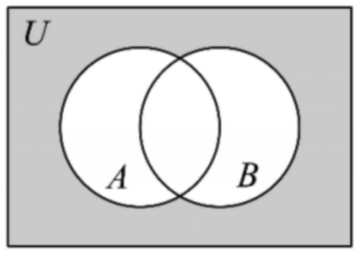
\includegraphics[width=0.20\textwidth]{figures/gao84_q9_venn.png}
\end{center}

\ifanswer
\solbegin
\step{$U=\{1,2,3,4,5,6,7,8,9,10\}$，$A=\{1,2\}$，$B=\{2,4\}$.}
\step{图中阴影部分表示的集合为 $\overline{A\cup B}=\{3,5,6,7,8,9,10\}$，共 $7$ 个元素，}
\step{其非空真子集的个数为 $2^7-2=126$.}
\solend
\fi

\item 若不等式 $ax^2-5x+c<0$ 的解集是 $(2,3)$，则不等式 $cx^2+5x+a\geqslant0$ 的解集是\blankline[4.4em].

\ifanswer
\solbegin
\step{若不等式 $ax^2-5x+c<0$ 的解集是 $(2,3)$，则 $a>0$ 且 $\begin{cases}\dfrac5a=5\\[2pt] \dfrac ca=6\end{cases}$，}
\step{则 $a=1$，$c=6$，}
\step{则不等式 $cx^2+5x+a\geqslant0$ 可化为 $6x^2+5x+1\geqslant0$，则 $x\leqslant-\dfrac12$ 或 $x\geqslant-\dfrac13$，}
\step{则不等式的解集为 $\left(-\infty,-\dfrac12\right]\cup\left[-\dfrac13,+\infty\right)$.}
\solend
\fi

\item 若关于 $x$ 的方程 $mx^2+2x+2=0$ 至少有一个负实根，则实数 $m$ 的取值范围是\blankline[4.4em].

\ifanswer
\solbegin
\step{①当 $m=0$ 时，方程为 $2x+2=0$，有一个负根，满足题意，}
\step{②当 $m\neq0$ 时，关于 $x$ 的方程 $mx^2+2x+2=0$ 至少有一个负根，}
\step{设根为 $x_1$、$x_2$，}
\step{当 $\Delta=4-8m=0$ 时，即 $m=\dfrac12$ 时，方程为 $\dfrac12x^2+2x+1=0$，}
\step{解得 $x=-2$，满足题意，}
\step{当 $\Delta=4-8m>0$，即 $m<\dfrac12$ 时，且 $m\neq0$ 时，}
\step{若有一个负根，则 $x_1x_2=\dfrac2m<0$，解得 $m<0$，}
\step{若有两个负根，则 $\begin{cases}x_1+x_2=-\dfrac2m<0\\[2pt] x_1x_2=\dfrac2m>0\end{cases}$，解得 $0<m<\dfrac12$，}
\step{综上所述，则实数 $m$ 的取值范围是 $\left(-\infty,\dfrac12\right]$.}
\solend
\fi

\item 设集合 $S$、$T$ 都至少含有两个元素，且 $S$、$T$ 同时满足：条件 1：对任意 $x$、$y\in S$，若
$x\neq y$，则 $x+y\in T$；条件 2：对任意 $x$、$y\in T$，若 $x\neq y$，则 $x-y\in S$. 给出下列说法：

①若 $S$ 只有 $2$ 个元素，则这 $2$ 个元素互为相反数；

②若 $S$ 只有 $2$ 个元素，则 $S\cup T$ 必有 $3$ 个元素；

③若 $S$ 只有 $2$ 个元素，则 $S\cup T$ 可能有 $4$ 个元素；

④存在含有 $3$ 个元素的集合 $S$，满足 $S\cup T$ 有 $4$ 个元素.

其中所有正确说法的序号是\blankline[4.4em].

\ifanswer
\solbegin
\step{对于①：由条件 2 得 $x-y\in S$，$y-x\in S$，且 $x-y\neq y-x$，}
\step{所以若 $S$ 只有 $2$ 个元素，则这 $2$ 个元素互为相反数，故①正确；}
\step{对于④：若 $S$ 有 $3$ 个元素，不妨设 $S=\{a,b,c\}$，其中 $a<b<c$，}
\step{则 $\{a+b,b+c,c+a\}\subseteq T$，所以 $c-a$、$c-b$、$b-a$、$a-c$、$b-c$、$a-b\in S$，}
\step{而 $c-a$ 与 $c-b$ 为两个互不相等的正数，$a-c$ 与 $a-b$ 为两个互不相等的负数，}
\step{故集合 $S$ 中至少有 $4$ 个元素，与 $S=\{a,b,c\}$ 有 $3$ 个元素矛盾，故④错误.}
\step{对于②③：若 $S$ 有 $2$ 个元素，由①得集合 $S$ 中的 $2$ 个元素必为相反数，}
\step{故可设 $S=\{a,-a\}(a\neq0)$. 由条件 1 得 $0\in T$，}
\step{由于集合 $T$ 中至少有 $2$ 个元素，故至少还有另外一个元素 $m\in T$.}
\step{当集合 $T$ 只有 $2$ 个元素时即 $T=\{0,m\}$，由条件 1 得 $-m\in S$，则 $m=\pm a$，}
\step{$T=\{0,a\}$ 或 $T=\{0,-a\}$，故 $S\cup T=\{0,a,-a\}$.}
\step{当集合 $T$ 有多于 $2$ 个元素时，不妨设 $T=\{0,m,n\}$，}
\step{则 $m$、$n$、$-m$、$-n$、$m-n$、$n-m\in S$，由于 $m$、$n\neq0$，}
\step{所以 $m\neq m-n$，$n\neq n-m$，又 $m\neq n$，}
\step{故集合 $S$ 至少有 $3$ 个元素，与 $S$ 中只有两个元素矛盾.}
\step{综上，$S\cup T=\{0,a,-a\}$，故②正确，③错误.}
\step{故正确的是①②.}
\solend
\fi

\end{enumerate}

\bigsec{二、选择题}

\begin{enumerate}
\setcounter{enumi}{12}

\item 用反证法证明命题：“若 $x+y>2$，则 $x>1$ 或 $y>1$”时，应假设\mbox{（\quad）}

\keepwithprev
A. $x\leqslant1$ 或 $y\leqslant1$\qquad B. 若 $x>1$ 或 $y>1$

C. $x\leqslant1$ 且 $y\leqslant1$\qquad D. 若 $x>1$ 且 $y>1$

\ifanswer
\ans{$C$}
\fi

\item 下列命题中，为真命题的是\mbox{（\quad）}

\keepwithprev
A. 若 $a>b$，则 $a^2>b^2$\qquad B. 若 $a>b$，$c>d$，则 $ac>bd$

C. 若 $a>b$，则 $\dfrac1a<\dfrac1b$\qquad D. 若 $ac^2>bc^2$，则 $a>b$

\ifanswer
\solbegin
\step{对于 $A$，当 $a=-1$，$b=-2$ 时，$a^2<b^2$，故 $A$ 错误；}
\step{对于 $B$，当 $a=-1$，$b=-2$，$c=-1$，$d=-2$ 时，$ac<bd$，故 $B$ 错误；}
\step{对于 $C$，当 $a=1$，$b=-2$ 时，$\dfrac1a>\dfrac1b$，故 $C$ 错误；}
\step{对于 $D$，因为 $ac^2-bc^2=(a-b)c^2>0$，所以 $a-b>0$，$c^2>0$，则 $a>b$，}
\step{故 $D$ 正确.}
\step{故选 $D$.}
\solend
\fi

\item 现有一级小麦 $m\,\mathrm{kg}$，二级小麦 $n\,\mathrm{kg}$，某粮食收购站有两种收购方案. 方案一：分两个
等级收购小麦，一级小麦 $a$ 元$/\mathrm{kg}$，二级小麦 $b$ 元$/\mathrm{kg}\,(b<a)$；方案二：以方案一两种价
格的平均数收购. 收购方式更加优惠的是\mbox{（\quad）}

\keepwithprev
A. 方案一\qquad B. 方案二\qquad C. 同样优惠\qquad D. 以上均有可能

\ifanswer
\solbegin
\step{方案一收购的平均价格为 $\dfrac{ma+nb}{m+n}$，方案二收购的平均价格为 $\dfrac{a+b}2$；}
\step{所以 $\dfrac{ma+nb}{m+n}-\dfrac{a+b}2=\dfrac{(a-b)(m-n)}{2(m+n)}$ ①，}
\step{$a-b>0$，$m-n$ 的正负性不确定，故①式的正负性不确定，故选 $D$.}
\solend
\fi

\item 用 $C(A)$ 表示非空集合 $A$ 中的元素个数. 对于集合 $A$、$B$，定义

$A*B=\begin{cases}C(A)-C(B),&C(A)\geqslant C(B)\\ C(B)-C(A),&C(A)<C(B)\end{cases}$，若 $A=\{0,1\}$，

$B=\{x\mid(x^2-ax)(x^2+ax+2)=0\}$，设实数 $a$ 的所有可能取值组成的集合是 $S$，则下列选
项不正确的是\mbox{（\quad）}

\keepwithprev
A. $C(B)$ 的可能值为 $1$，$2$，$3$，$4$

B. 若 $A*B=2$，则 $a$ 的取值范围为 $(-\infty,-2\sqrt2)\cup(2\sqrt2,+\infty)$

C. 若 $A*B=1$，则 $C(S)=3$

D. 若 $A*B=0$，则 $a$ 的取值范围为 $(-2\sqrt2,2\sqrt2)$

\ifanswer
\solbegin
\step{对于集合 $B$，当 $a=0$ 时，方程 $x^2(x^2+2)=0$ 的解为 $x=0$，$C(B)=1$，}
\step{当 $a\neq0$ 时，$x^2-ax=0$ 或 $x^2+ax+2=0$，}
\step{其中 $x^2-ax=0$ 的解为 $x_1=0$，$x_2=a$，}
\step{若 $\Delta=a^2-8>0$，即 $a>2\sqrt2$ 或 $a<-2\sqrt2$，}
\step{方程 $x^2+ax+2=0$ 有两个不相等的实数根，此时 $C(B)=4$；}
\step{若 $\Delta=a^2-8=0$，即 $a=2\sqrt2$ 或 $-2\sqrt2$，}
\step{方程 $x^2+ax+2=0$ 有两个相等的实数根，此时 $C(B)=3$；}
\step{若 $\Delta=a^2-8<0$，即 $-2\sqrt2<a<0$ 或 $0<a<2\sqrt2$，}
\step{方程 $x^2+ax+2=0$ 无实数根，此时 $C(B)=2$；}
\step{所以 $C(B)$ 的可能值为 $1$，$2$，$3$，$4$，故 $A$ 正确；}
\step{若 $A*B=2$，且 $C(A)=2$，则 $C(B)=4$，}
\step{则 $a$ 的取值范围 $(-\infty,-2\sqrt2)\cup(2\sqrt2,+\infty)$，故 $B$ 正确；}
\step{若 $A*B=1$，且 $C(A)=2$，则 $C(B)=1$ 或 $3$，}
\step{当 $C(B)=1$ 时，$a=0$，}
\step{当 $C(B)=3$ 时，$a=2\sqrt2$ 或 $-2\sqrt2$，此时集合 $S=\{0,-2\sqrt2,2\sqrt2\}$，}
\step{则 $C(S)=3$，故 $C$ 正确；}
\step{若 $A*B=0$，且 $C(A)=2$，则 $C(B)=2$，}
\step{由此可得 $a$ 的取值范围为 $(-2\sqrt2,0)\cup(0,2\sqrt2)$，故 $D$ 不正确；}
\step{故选 $D$.}
\solend
\fi

\end{enumerate}

\bigsec{三、解答题}

\begin{enumerate}
\setcounter{enumi}{16}

\item 已知集合 $A=\{x\mid-3<x\leqslant4\}$，集合 $B=\{x\mid k+1\leqslant x\leqslant2k-1\}$.

（1）当 $k=3$ 时，求 $A\cup B$、$\overline A\cap B$；

（2）若 $B\subseteq A$，求 $k$ 的取值范围.

\ansspace*[10]

\ifanswer
\solbegin
\stepm{（1）}{当 $k=3$ 时，$B=\{x\mid4\leqslant x\leqslant5\}$，又 $A=\{x\mid-3<x\leqslant4\}$，}
\step{所以 $\overline A=\{x\mid x\leqslant-3$ 或 $x>4\}$，}
\step{所以 $A\cup B=\{x\mid-3<x\leqslant5\}$，$\overline A\cap B=\{x\mid4<x\leqslant5\}$.}
\stepm{（2）}{①当 $B=\varnothing$，即 $k+1>2k-1$ 时，$k<2$，满足 $B\subseteq A$.}
\step{②当 $B\neq\varnothing$ 时，由 $B\subseteq A$ 得 $\begin{cases}k+1\leqslant2k-1\\ k+1>-3\\ 2k-1\leqslant4\end{cases}$，解得 $2\leqslant k\leqslant\dfrac52$，}
\step{综合①②得 $k$ 的取值范围 $\left\{k\mid k\leqslant\dfrac52\right\}$.}
\solend
\fi

\item 设集合 $A=\{x\mid x^2-3x+2=0\}$，$B=\{x\mid x^2+2(a+1)x+a^2-5=0\}$.

（1）若 $A\cap B=\{2\}$，求实数 $a$ 的值；

（2）若集合 $B$ 中有两个元素 $x_1,x_2$，求 $\lvert x_1-x_2\rvert$（用 $a$ 表示）.

\ansspace*[10]

\ifanswer
\solbegin
\stepm{（1）}{由题意得 $A=\{x\mid x^2-3x+2=0\}=\{1,2\}$，因为 $A\cap B=\{2\}$，所以 $2\in B$，}
\step{所以 $2^2+4(a+1)+a^2-5=0$ 即 $4+4a+4+a^2-5=0$，}
\step{化简得 $a^2+4a+3=0$，即 $(a+3)(a+1)=0$，解得 $a=-3$ 或 $a=-1$，}
\step{检验：当 $a=-3$ 时，$B=\{x\mid x^2-4x+4=0\}=\{2\}$，满足 $A\cap B=\{2\}$，}
\step{当 $a=-1$ 时，$B=\{x\mid x^2-4=0\}=\{-2,2\}$，满足 $A\cap B=\{2\}$，}
\step{所以 $a=-3$ 或 $a=-1$.}
\stepm{（2）}{因为 $B$ 中有两个元素 $x_1,x_2$，所以 $x^2+2(a+1)x+(a^2-5)=0$ 有两个根，}
\step{所以 $\Delta=4(a+1)^2-4(a^2-5)=8a+24>0$，}
\step{且 $x_1+x_2=-2(a+1)$，$x_1x_2=a^2-5$，}
\step{所以 $\lvert x_1-x_2\rvert=\sqrt{(x_1+x_2)^2-4x_1x_2}=\sqrt{4(a+1)^2-4(a^2-5)}=\sqrt{8a+24}$.}
\solend
\fi

\item 已知关于 $x$ 的不等式 $\dfrac{ax-2}{1+x}>0$.

（1）若 $x=-a$ 时，不等式成立，求实数 $a$ 的取值范围；

（2）若 $a$ 为实数，解关于 $x$ 的不等式：$\dfrac{ax-2}{1+x}>0$.

\ansspace*[12]

\ifanswer
\solbegin
\stepm{（1）}{因为 $x=-a$ 时，不等式成立，}
\step{所以 $\dfrac{-a^2-2}{1-a}>0\Rightarrow\dfrac{a^2+2}{a-1}>0\Rightarrow a-1>0\Rightarrow a>1$，}
\step{所以实数 $a$ 的取值范围为 $(1,+\infty)$.}
\stepm{（2）}{$\dfrac{ax-2}{1+x}>0\Rightarrow(ax-2)(x+1)>0$，}
\step{当 $a=0$ 时，$-2(x+1)>0$，解得 $x<-1$.}
\step{当 $a>0$ 时，$(ax-2)(x+1)>0$，解得 $x>\dfrac2a$ 或 $x<-1$.}
\step{当 $a<0$ 时，不等式 $(ax-2)(x+1)>0$ 可化为 $\left(x-\dfrac2a\right)(x+1)<0$，}
\step{当 $\dfrac2a>-1$，即 $a<-2$ 时，解得 $-1<x<\dfrac2a$；}
\step{当 $\dfrac2a<-1$，即 $-2<a<0$ 时，解得 $\dfrac2a<x<-1$；}
\step{当 $\dfrac2a=-1$，即 $a=-2$ 时，解集为 $\varnothing$.}
\step{综上，当 $a<-2$ 时，不等式的解集为 $\left(-1,\dfrac2a\right)$；}
\step{当 $a=-2$ 时，不等式的解集为 $\varnothing$；}
\step{当 $-2<a<0$ 时，不等式的解集为 $\left(\dfrac2a,-1\right)$；}
\step{当 $a=0$ 时，不等式的解集为 $(-\infty,-1)$；}
\step{当 $a>0$ 时，不等式的解集为 $(-\infty,-1)\cup\left(\dfrac2a,+\infty\right)$.}
\solend
\fi

\item 已知关于 $x$ 的不等式 $(k^2-2k-3)x^2+(k+1)x+1>0\,(k\in\R)$ 的解集为 $M$；

（1）若存在实数 $a$，使得 $M=(-\infty,a)\cup(a,+\infty)$，求 $k$ 的值；

（2）若 $M=\R$，求 $k$ 的取值范围；

（3）是否存在实数 $k$，满足：“对于任意 $n\in\N$，$n>0$，都有 $n\in M$；对于任意
$m\in\Z$，$m<0$，都有 $m\notin M$”，若存在，求出 $k$ 的值，若不存在，说明理由.

\ansspace*[13]

\ifanswer
\solbegin
\stepm{（1）}{记 $f(x)=(k^2-2k-3)x^2+(k+1)x+1$.}
\step{$M=(-\infty,a)\cup(a,+\infty)$ 表示 $f(x)>0$ 对一切 $x\neq a$ 成立，且 $f(a)=0$，}
\step{故需二次项系数大于 $0$ 且 $\Delta=0$.}
\step{由 $\Delta=(k+1)^2-4(k^2-2k-3)=-3k^2+10k+13=0$ 得 $k=\dfrac{13}3$ 或 $k=-1$.}
\step{当 $k=\dfrac{13}3$ 时，二次项系数 $\dfrac{64}9>0$，$f(x)=\dfrac{64}9\left(x+\dfrac38\right)^2$，符合；}
\step{当 $k=-1$ 时二次项系数为 $0$，$f(x)=1>0$，$M=\R$，不符合. 故 $k=\dfrac{13}3$.}
\stepm{（2）}{$M=\R$ 即 $f(x)>0$ 对一切 $x\in\R$ 恒成立.}
\step{①当 $k^2-2k-3>0$（即 $k<-1$ 或 $k>3$）时，需 $\Delta<0$，}
\step{即 $-3k^2+10k+13<0$，得 $k<-1$ 或 $k>\dfrac{13}3$，故 $k<-1$ 或 $k>\dfrac{13}3$；}
\step{②当 $k^2-2k-3=0$ 时，$k=3$ 得 $f(x)=4x+1$ 不恒正，不符合题意，}
\step{舍去，}
\step{当 $k=-1$ 得 $f(x)=1>0$ 恒成立，符合题意；}
\step{③当 $k^2-2k-3<0$ 时，抛物线开口向下，不能恒正.}
\step{综上，$k\leqslant-1$ 或 $k>\dfrac{13}3$.}
\stepm{（3）}{存在，$k=3$，理由如下，}
\step{由题意得解集 $M=(t,+\infty)$，$t\in[-1,1)$；}
\step{当 $k^2-2k-3=0$ 时，解得 $k=3$ 或 $k=-1$，}
\step{$k=3$ 时，不等式的解集为 $\left(-\dfrac14,+\infty\right)$，满足条件；}
\step{$k=-1$ 时，$1>0$ 恒成立，不满足条件；}
\step{当 $k^2-2k-3>0$ 时，}
\step{此时对应的一元二次不等式的解集形式不是 $(t,+\infty)$ 的形式，不满足条件；}
\step{当 $k^2-2k-3<0$ 时，}
\step{此时对应的一元二次不等式的解集形式不是 $(t,+\infty)$ 的形式，不满足条件；}
\step{综上，满足条件 $k$ 的值为 $3$.}
\solend
\fi

\item 已知有限集 $A=\{a_1,a_2,\cdots,a_n\}\,(n\geqslant2,n\in\N)$，如果 $A$ 中元素 $a_i\,(i=1,2,3,\cdots,n)$ 满足
$a_1+a_2+a_3+\cdots+a_n=a_1\times a_2\times\cdots\times a_n$，就称 $A$ 为“和积平衡集”.

（1）判断集合 $\{-1+\sqrt3,-1-\sqrt3\}$ 是否为“和积平衡集”；

（2）若 $a_1$、$a_2$ 是两个不同的正数，且 $\{a_1,a_2\}$ 是“和积平衡集”，写出以 $a_1$、$a_2$ 为根的一
个一元二次方程（系数可用 $a_1$、$a_2$ 表示），并证明 $a_1$、$a_2$ 至少有一个大于 $2$；

（3）若 $a_i\in\Z$ 且 $a_i>0$，求所有符合条件的“和积平衡集”.

\ansspace*[14]

\ifanswer
\solbegin
\stepm{（1）}{对于集合 $\{-1+\sqrt3,-1-\sqrt3\}$，}
\step{因为 $(-1+\sqrt3)+(-1-\sqrt3)=-2$，$(-1+\sqrt3)\times(-1-\sqrt3)=-2$，}
\step{所以满足 $a_1+a_2=a_1\times a_2$，满足题意，}
\step{所以集合 $\{-1+\sqrt3,-1-\sqrt3\}$ 是和积平衡集.}
\stepm{（2）}{以 $a_1$、$a_2$ 为根的一个一元二次方程可为 $x^2-(a_1+a_2)x+a_1\cdot a_2=0$，}
\step{因为 $a_1$、$a_2$ 是两个不同的正数，且 $\{a_1,a_2\}$ 是和积平衡集，}
\step{所以 $a_1+a_2=a_1\cdot a_2$，}
\step{又 $a_1$ 和 $a_2$ 为 $x^2-(a_1+a_2)x+a_1\cdot a_2=0$ 的两个不同的正根，}
\step{所以 $\Delta=(a_1+a_2)^2-4a_1a_2=(a_1+a_2)^2-4(a_1+a_2)>0$，}
\step{又 $a_1+a_2>0$，则 $a_1+a_2>4$，}
\step{若 $a_1$、$a_2$ 都小于等于 $2$，则 $a_1+a_2\leqslant4$，矛盾，}
\step{所以 $a_1$、$a_2$ 至少有一个大于 $2$；}
\stepm{（3）}{设 $A$ 中的 $a_1<a_2<a_3<\cdots<a_n$，且 $a_i\in\N^*$，}
\step{由 $a_1+a_2+a_3+\cdots+a_n=a_1\times a_2\times\cdots\times a_n$，得 $n=2$ 时明显不满足，}
\step{所以 $n\geqslant3$，故 $a_1\times a_2\times\cdots\times a_n=a_1+a_2+a_3+\cdots+a_n\leqslant na_n$，}
\step{所以 $a_1\times a_2\times\cdots\times a_{n-1}\leqslant n$，}
\step{当 $n=3$ 时，$a_1\times a_2\leqslant3$，$a_i\in\N^*$，只能有 $a_1=1$，$a_2=2$，}
\step{由 $a_1+a_2+a_3=a_1\times a_2\times a_3$，得 $a_3=3$，此时的和积平衡集为 $\{1,2,3\}$，}
\step{当 $n\geqslant4$ 时，$a_1\times a_2\times\cdots\times a_{n-1}\geqslant(n-1)(n-2)\times\cdots\times2\times1\geqslant(n-1)(n-2)$，}
\step{又 $(n-1)(n-2)-n=n^2-4n+2=n(n-4)+2>0$，即 $(n-1)(n-2)>n$，}
\step{即 $a_1\times a_2\times\cdots\times a_{n-1}>n$，与 $a_1\times a_2\times\cdots\times a_{n-1}\leqslant n$ 矛盾，}
\step{所以 $n\geqslant4$ 不满足条件，}
\step{所以符合条件的和积平衡集有且只有 $n=3$，此时的和积平衡集为 $\{1,2,3\}$.}
\solend
\fi

\end{enumerate}

\end{document}
"
%
% 原始材料：微信公众号“魔都数学加油站”文章，连载“27学年高一84”；
% 原文标题“27学年高一84——2026-2027年上海市东昌中学高一上10月月考”；
% 原文链接：https://mp.weixin.qq.com/s/PErsjO3N5RsMuJC69IGbrw。
% 页面标注发布时间 2026-10-26 20:15（上海）。
% 正文为 12 张 PNG 页（`原图/高一84_东昌中学_10月月考/01..12.png`），
% 尺寸混排（第 1—8 页为 4762×6735，第 9—12 页为 2560×3620），均按页序读取。
%
% 篇幅与题号：原卷自第 3 题起编号（第 1、2 题不在原文内）。填空题 3—12（10 题）、
% 选择题 13—16（4 题）、解答题 17—21（5 题），共 19 题。
%
% 讲评版：19 题全部印【解析】，本稿不另提 \ans{}；选择题答案在解析末句“故选 D／C／D”。
% 第 13 题的答案“C”原卷直接印在题干括号内（“（\ C\ ）”），本稿按 高一37 第 13 题／
% 高一63 第 14 题成例括号留空、另提 \ans{$C$}（该题无【解析】段）。
%
% 副标题：原卷未印副标题。本稿按内容标作“集合与常用逻辑用语、不等式”。
%
% 与原卷的排版差异：
%   ① 原卷每题下直接印【解析】，本稿按全稿惯例将解析置于答案版；
%   ② 原卷未印副标题，本稿补出；填空横线统一排 \blankline[4.4em]；
%   ③ 原卷数集记号排斜体 $R$、$Z$、$N$，本稿按全稿惯例改用 $\R$、$\Z$、$\N$；
%   ④ 第 17—21 题的子问用行内“（1）（2）（3）”段，解析中的子问标号用 \stepm；
%   ⑤ 解答题按惯例加 \ansspace；选择题括号排 \mbox{（\quad）}；
%   ⑥ 第 9 题题干右侧有一幅韦恩图，裁自原图（第 2 页）后去粉色水印、转灰度，
%      三版都出（属题干）。
%
% 行数核对：逐题数 \step/\stepm 条数，合计 157 条（Q3：2；Q4：2；Q5：3；Q6：2；
% Q7：3；Q8：6；Q9：3；Q10：4；Q11：9；Q12：17；Q14：6；Q15：3；Q16：19；
% Q17：6；Q18：10；Q19：15；Q20：24；Q21：23）；第 13 题无解析，只提 \ans{}，
% 不计入 \step 账。原卷解析的换行按语意合并，未逐行强拆。
%
\documentclass[a4paper,11pt]{article}
\usepackage{common}

\begin{document}

\examtitlest[4]{2026--2027 年东昌中学高一上 10 月月考}{集合与常用逻辑用语、不等式}

\bigsec{一、填空题}

\begin{enumerate}
\setcounter{enumi}{2}

\item 若 $a\in\R$，则“$a=2$”是“$(a-1)(a-2)=0$”的\blankline[3.6em]条件（填“充分不必要”、“必要
不充分”、“充要”、“既不充分又不必要”的一个）.

\ifanswer
\solbegin
\step{$a=2\Rightarrow(a-1)(a-2)=0$，而 $(a-1)(a-2)=0$ 不能推出 $a=2$，}
\step{故“$a=2$”是“$(a-1)(a-2)=0$”的充分不必要条件.}
\solend
\fi

\item 已知集合 $M=\{(x,y)\mid y=x^2\}$，$N=\{(x,y)\mid y=1\}$，则 $M\cap N=\blankline[4.4em]$.

\ifanswer
\solbegin
\step{集合 $M=\{(x,y)\mid y=x^2\}$，$N=\{(x,y)\mid y=1\}$，}
\step{当 $y=1$ 时，$x=\pm1$，则 $M\cap N=\{(-1,1),(1,1)\}$.}
\solend
\fi

\item 已知集合 $A=\{x\mid x^2+ax+4=0\}$，若 $A$ 有且只有一个非空子集，则实数 $a=\blankline[4.4em]$.

\ifanswer
\solbegin
\step{因为集合 $A$ 有且只有一个非空子集，所以集合 $A$ 中只有一个元素，}
\step{所以一元二次方程 $x^2+ax+4=0$ 有两个相等的解，}
\step{所以 $\Delta=a^2-4\times4=0$，解得 $a=\pm4$.}
\solend
\fi

\item 已知 $A=(-\infty,a]$，$B=(-\infty,3)$，且 $x\in A$ 是 $x\in B$ 的充分不必要条件，则 $a$ 的取值范围
是\blankline[4.4em].

\ifanswer
\solbegin
\step{$A=(-\infty,a]$，$B=(-\infty,3)$，且 $x\in A$ 是 $x\in B$ 的充分不必要条件，}
\step{则 $A\subset B$，则 $a<3$，即 $a$ 的取值范围为 $(-\infty,3)$.}
\solend
\fi

\item 不等式 $\dfrac{3x-1}{x-2}\leqslant1$ 的解集为\blankline[4.4em].

\ifanswer
\solbegin
\step{由 $\dfrac{3x-1}{x-2}\leqslant1$，得 $\dfrac{3x-1}{x-2}-1=\dfrac{3x-1-(x-2)}{x-2}=\dfrac{2x+1}{x-2}\leqslant0$，}
\step{则 $\begin{cases}(2x+1)(x-2)\leqslant0\\ x-2\neq0\end{cases}$，解得 $-\dfrac12\leqslant x<2$，}
\step{则不等式 $\dfrac{3x-1}{x-2}\leqslant1$ 的解集为 $\left[-\dfrac12,2\right)$.}
\solend
\fi

\item 已知关于 $x$ 的一元二次方程 $x^2-2mx+(3m+1)=0$ 的两个实数根为 $x_1$、$x_2$，且
$x_1^2+x_2^2=16$，则实数 $m$ 的值为\blankline[4.4em].

\ifanswer
\solbegin
\step{由韦达定理，得 $x_1+x_2=2m$，$x_1x_2=3m+1$，}
\step{$x_1^2+x_2^2=(x_1+x_2)^2-2x_1x_2=4m^2-6m-2$，}
\step{由 $x_1^2+x_2^2=16$，得 $4m^2-6m-2=16$，即 $2m^2-3m-9=0$，}
\step{解得 $m=3$ 或 $m=-\dfrac32$，}
\step{检验判别式 $\Delta=4m^2-12m-4$，当 $m=3$ 时，$\Delta=-4<0$，舍去；}
\step{当 $m=-\dfrac32$ 时，$\Delta=23>0$，符合条件，故 $m=-\dfrac32$.}
\solend
\fi

\item 已知全集 $U=\{x\mid1\leqslant x\leqslant10,\,x\in\N\}$，集合 $A=\{x\mid x^2-3<4,\,x\in\N,\,x>0\}$，
$B=\{2,4\}$，则图中阴影部分表示的集合的非空真子集个数为\blankline[4.4em].

\needvspace{9\baselineskip}
\begin{center}
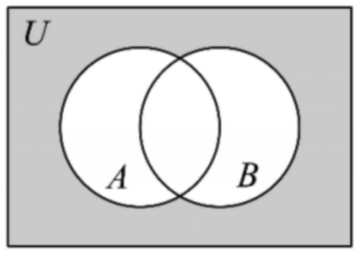
\includegraphics[width=0.20\textwidth]{figures/gao84_q9_venn.png}
\end{center}

\ifanswer
\solbegin
\step{$U=\{1,2,3,4,5,6,7,8,9,10\}$，$A=\{1,2\}$，$B=\{2,4\}$.}
\step{图中阴影部分表示的集合为 $\overline{A\cup B}=\{3,5,6,7,8,9,10\}$，共 $7$ 个元素，}
\step{其非空真子集的个数为 $2^7-2=126$.}
\solend
\fi

\item 若不等式 $ax^2-5x+c<0$ 的解集是 $(2,3)$，则不等式 $cx^2+5x+a\geqslant0$ 的解集是\blankline[4.4em].

\ifanswer
\solbegin
\step{若不等式 $ax^2-5x+c<0$ 的解集是 $(2,3)$，则 $a>0$ 且 $\begin{cases}\dfrac5a=5\\[2pt] \dfrac ca=6\end{cases}$，}
\step{则 $a=1$，$c=6$，}
\step{则不等式 $cx^2+5x+a\geqslant0$ 可化为 $6x^2+5x+1\geqslant0$，则 $x\leqslant-\dfrac12$ 或 $x\geqslant-\dfrac13$，}
\step{则不等式的解集为 $\left(-\infty,-\dfrac12\right]\cup\left[-\dfrac13,+\infty\right)$.}
\solend
\fi

\item 若关于 $x$ 的方程 $mx^2+2x+2=0$ 至少有一个负实根，则实数 $m$ 的取值范围是\blankline[4.4em].

\ifanswer
\solbegin
\step{①当 $m=0$ 时，方程为 $2x+2=0$，有一个负根，满足题意，}
\step{②当 $m\neq0$ 时，关于 $x$ 的方程 $mx^2+2x+2=0$ 至少有一个负根，}
\step{设根为 $x_1$、$x_2$，}
\step{当 $\Delta=4-8m=0$ 时，即 $m=\dfrac12$ 时，方程为 $\dfrac12x^2+2x+1=0$，}
\step{解得 $x=-2$，满足题意，}
\step{当 $\Delta=4-8m>0$，即 $m<\dfrac12$ 时，且 $m\neq0$ 时，}
\step{若有一个负根，则 $x_1x_2=\dfrac2m<0$，解得 $m<0$，}
\step{若有两个负根，则 $\begin{cases}x_1+x_2=-\dfrac2m<0\\[2pt] x_1x_2=\dfrac2m>0\end{cases}$，解得 $0<m<\dfrac12$，}
\step{综上所述，则实数 $m$ 的取值范围是 $\left(-\infty,\dfrac12\right]$.}
\solend
\fi

\item 设集合 $S$、$T$ 都至少含有两个元素，且 $S$、$T$ 同时满足：条件 1：对任意 $x$、$y\in S$，若
$x\neq y$，则 $x+y\in T$；条件 2：对任意 $x$、$y\in T$，若 $x\neq y$，则 $x-y\in S$. 给出下列说法：

①若 $S$ 只有 $2$ 个元素，则这 $2$ 个元素互为相反数；

②若 $S$ 只有 $2$ 个元素，则 $S\cup T$ 必有 $3$ 个元素；

③若 $S$ 只有 $2$ 个元素，则 $S\cup T$ 可能有 $4$ 个元素；

④存在含有 $3$ 个元素的集合 $S$，满足 $S\cup T$ 有 $4$ 个元素.

其中所有正确说法的序号是\blankline[4.4em].

\ifanswer
\solbegin
\step{对于①：由条件 2 得 $x-y\in S$，$y-x\in S$，且 $x-y\neq y-x$，}
\step{所以若 $S$ 只有 $2$ 个元素，则这 $2$ 个元素互为相反数，故①正确；}
\step{对于④：若 $S$ 有 $3$ 个元素，不妨设 $S=\{a,b,c\}$，其中 $a<b<c$，}
\step{则 $\{a+b,b+c,c+a\}\subseteq T$，所以 $c-a$、$c-b$、$b-a$、$a-c$、$b-c$、$a-b\in S$，}
\step{而 $c-a$ 与 $c-b$ 为两个互不相等的正数，$a-c$ 与 $a-b$ 为两个互不相等的负数，}
\step{故集合 $S$ 中至少有 $4$ 个元素，与 $S=\{a,b,c\}$ 有 $3$ 个元素矛盾，故④错误.}
\step{对于②③：若 $S$ 有 $2$ 个元素，由①得集合 $S$ 中的 $2$ 个元素必为相反数，}
\step{故可设 $S=\{a,-a\}(a\neq0)$. 由条件 1 得 $0\in T$，}
\step{由于集合 $T$ 中至少有 $2$ 个元素，故至少还有另外一个元素 $m\in T$.}
\step{当集合 $T$ 只有 $2$ 个元素时即 $T=\{0,m\}$，由条件 1 得 $-m\in S$，则 $m=\pm a$，}
\step{$T=\{0,a\}$ 或 $T=\{0,-a\}$，故 $S\cup T=\{0,a,-a\}$.}
\step{当集合 $T$ 有多于 $2$ 个元素时，不妨设 $T=\{0,m,n\}$，}
\step{则 $m$、$n$、$-m$、$-n$、$m-n$、$n-m\in S$，由于 $m$、$n\neq0$，}
\step{所以 $m\neq m-n$，$n\neq n-m$，又 $m\neq n$，}
\step{故集合 $S$ 至少有 $3$ 个元素，与 $S$ 中只有两个元素矛盾.}
\step{综上，$S\cup T=\{0,a,-a\}$，故②正确，③错误.}
\step{故正确的是①②.}
\solend
\fi

\end{enumerate}

\bigsec{二、选择题}

\begin{enumerate}
\setcounter{enumi}{12}

\item 用反证法证明命题：“若 $x+y>2$，则 $x>1$ 或 $y>1$”时，应假设\mbox{（\quad）}

\keepwithprev
A. $x\leqslant1$ 或 $y\leqslant1$\qquad B. 若 $x>1$ 或 $y>1$

C. $x\leqslant1$ 且 $y\leqslant1$\qquad D. 若 $x>1$ 且 $y>1$

\ifanswer
\ans{$C$}
\fi

\item 下列命题中，为真命题的是\mbox{（\quad）}

\keepwithprev
A. 若 $a>b$，则 $a^2>b^2$\qquad B. 若 $a>b$，$c>d$，则 $ac>bd$

C. 若 $a>b$，则 $\dfrac1a<\dfrac1b$\qquad D. 若 $ac^2>bc^2$，则 $a>b$

\ifanswer
\solbegin
\step{对于 $A$，当 $a=-1$，$b=-2$ 时，$a^2<b^2$，故 $A$ 错误；}
\step{对于 $B$，当 $a=-1$，$b=-2$，$c=-1$，$d=-2$ 时，$ac<bd$，故 $B$ 错误；}
\step{对于 $C$，当 $a=1$，$b=-2$ 时，$\dfrac1a>\dfrac1b$，故 $C$ 错误；}
\step{对于 $D$，因为 $ac^2-bc^2=(a-b)c^2>0$，所以 $a-b>0$，$c^2>0$，则 $a>b$，}
\step{故 $D$ 正确.}
\step{故选 $D$.}
\solend
\fi

\item 现有一级小麦 $m\,\mathrm{kg}$，二级小麦 $n\,\mathrm{kg}$，某粮食收购站有两种收购方案. 方案一：分两个
等级收购小麦，一级小麦 $a$ 元$/\mathrm{kg}$，二级小麦 $b$ 元$/\mathrm{kg}\,(b<a)$；方案二：以方案一两种价
格的平均数收购. 收购方式更加优惠的是\mbox{（\quad）}

\keepwithprev
A. 方案一\qquad B. 方案二\qquad C. 同样优惠\qquad D. 以上均有可能

\ifanswer
\solbegin
\step{方案一收购的平均价格为 $\dfrac{ma+nb}{m+n}$，方案二收购的平均价格为 $\dfrac{a+b}2$；}
\step{所以 $\dfrac{ma+nb}{m+n}-\dfrac{a+b}2=\dfrac{(a-b)(m-n)}{2(m+n)}$ ①，}
\step{$a-b>0$，$m-n$ 的正负性不确定，故①式的正负性不确定，故选 $D$.}
\solend
\fi

\item 用 $C(A)$ 表示非空集合 $A$ 中的元素个数. 对于集合 $A$、$B$，定义

$A*B=\begin{cases}C(A)-C(B),&C(A)\geqslant C(B)\\ C(B)-C(A),&C(A)<C(B)\end{cases}$，若 $A=\{0,1\}$，

$B=\{x\mid(x^2-ax)(x^2+ax+2)=0\}$，设实数 $a$ 的所有可能取值组成的集合是 $S$，则下列选
项不正确的是\mbox{（\quad）}

\keepwithprev
A. $C(B)$ 的可能值为 $1$，$2$，$3$，$4$

B. 若 $A*B=2$，则 $a$ 的取值范围为 $(-\infty,-2\sqrt2)\cup(2\sqrt2,+\infty)$

C. 若 $A*B=1$，则 $C(S)=3$

D. 若 $A*B=0$，则 $a$ 的取值范围为 $(-2\sqrt2,2\sqrt2)$

\ifanswer
\solbegin
\step{对于集合 $B$，当 $a=0$ 时，方程 $x^2(x^2+2)=0$ 的解为 $x=0$，$C(B)=1$，}
\step{当 $a\neq0$ 时，$x^2-ax=0$ 或 $x^2+ax+2=0$，}
\step{其中 $x^2-ax=0$ 的解为 $x_1=0$，$x_2=a$，}
\step{若 $\Delta=a^2-8>0$，即 $a>2\sqrt2$ 或 $a<-2\sqrt2$，}
\step{方程 $x^2+ax+2=0$ 有两个不相等的实数根，此时 $C(B)=4$；}
\step{若 $\Delta=a^2-8=0$，即 $a=2\sqrt2$ 或 $-2\sqrt2$，}
\step{方程 $x^2+ax+2=0$ 有两个相等的实数根，此时 $C(B)=3$；}
\step{若 $\Delta=a^2-8<0$，即 $-2\sqrt2<a<0$ 或 $0<a<2\sqrt2$，}
\step{方程 $x^2+ax+2=0$ 无实数根，此时 $C(B)=2$；}
\step{所以 $C(B)$ 的可能值为 $1$，$2$，$3$，$4$，故 $A$ 正确；}
\step{若 $A*B=2$，且 $C(A)=2$，则 $C(B)=4$，}
\step{则 $a$ 的取值范围 $(-\infty,-2\sqrt2)\cup(2\sqrt2,+\infty)$，故 $B$ 正确；}
\step{若 $A*B=1$，且 $C(A)=2$，则 $C(B)=1$ 或 $3$，}
\step{当 $C(B)=1$ 时，$a=0$，}
\step{当 $C(B)=3$ 时，$a=2\sqrt2$ 或 $-2\sqrt2$，此时集合 $S=\{0,-2\sqrt2,2\sqrt2\}$，}
\step{则 $C(S)=3$，故 $C$ 正确；}
\step{若 $A*B=0$，且 $C(A)=2$，则 $C(B)=2$，}
\step{由此可得 $a$ 的取值范围为 $(-2\sqrt2,0)\cup(0,2\sqrt2)$，故 $D$ 不正确；}
\step{故选 $D$.}
\solend
\fi

\end{enumerate}

\bigsec{三、解答题}

\begin{enumerate}
\setcounter{enumi}{16}

\item 已知集合 $A=\{x\mid-3<x\leqslant4\}$，集合 $B=\{x\mid k+1\leqslant x\leqslant2k-1\}$.

（1）当 $k=3$ 时，求 $A\cup B$、$\overline A\cap B$；

（2）若 $B\subseteq A$，求 $k$ 的取值范围.

\ansspace*[10]

\ifanswer
\solbegin
\stepm{（1）}{当 $k=3$ 时，$B=\{x\mid4\leqslant x\leqslant5\}$，又 $A=\{x\mid-3<x\leqslant4\}$，}
\step{所以 $\overline A=\{x\mid x\leqslant-3$ 或 $x>4\}$，}
\step{所以 $A\cup B=\{x\mid-3<x\leqslant5\}$，$\overline A\cap B=\{x\mid4<x\leqslant5\}$.}
\stepm{（2）}{①当 $B=\varnothing$，即 $k+1>2k-1$ 时，$k<2$，满足 $B\subseteq A$.}
\step{②当 $B\neq\varnothing$ 时，由 $B\subseteq A$ 得 $\begin{cases}k+1\leqslant2k-1\\ k+1>-3\\ 2k-1\leqslant4\end{cases}$，解得 $2\leqslant k\leqslant\dfrac52$，}
\step{综合①②得 $k$ 的取值范围 $\left\{k\mid k\leqslant\dfrac52\right\}$.}
\solend
\fi

\item 设集合 $A=\{x\mid x^2-3x+2=0\}$，$B=\{x\mid x^2+2(a+1)x+a^2-5=0\}$.

（1）若 $A\cap B=\{2\}$，求实数 $a$ 的值；

（2）若集合 $B$ 中有两个元素 $x_1,x_2$，求 $\lvert x_1-x_2\rvert$（用 $a$ 表示）.

\ansspace*[10]

\ifanswer
\solbegin
\stepm{（1）}{由题意得 $A=\{x\mid x^2-3x+2=0\}=\{1,2\}$，因为 $A\cap B=\{2\}$，所以 $2\in B$，}
\step{所以 $2^2+4(a+1)+a^2-5=0$ 即 $4+4a+4+a^2-5=0$，}
\step{化简得 $a^2+4a+3=0$，即 $(a+3)(a+1)=0$，解得 $a=-3$ 或 $a=-1$，}
\step{检验：当 $a=-3$ 时，$B=\{x\mid x^2-4x+4=0\}=\{2\}$，满足 $A\cap B=\{2\}$，}
\step{当 $a=-1$ 时，$B=\{x\mid x^2-4=0\}=\{-2,2\}$，满足 $A\cap B=\{2\}$，}
\step{所以 $a=-3$ 或 $a=-1$.}
\stepm{（2）}{因为 $B$ 中有两个元素 $x_1,x_2$，所以 $x^2+2(a+1)x+(a^2-5)=0$ 有两个根，}
\step{所以 $\Delta=4(a+1)^2-4(a^2-5)=8a+24>0$，}
\step{且 $x_1+x_2=-2(a+1)$，$x_1x_2=a^2-5$，}
\step{所以 $\lvert x_1-x_2\rvert=\sqrt{(x_1+x_2)^2-4x_1x_2}=\sqrt{4(a+1)^2-4(a^2-5)}=\sqrt{8a+24}$.}
\solend
\fi

\item 已知关于 $x$ 的不等式 $\dfrac{ax-2}{1+x}>0$.

（1）若 $x=-a$ 时，不等式成立，求实数 $a$ 的取值范围；

（2）若 $a$ 为实数，解关于 $x$ 的不等式：$\dfrac{ax-2}{1+x}>0$.

\ansspace*[12]

\ifanswer
\solbegin
\stepm{（1）}{因为 $x=-a$ 时，不等式成立，}
\step{所以 $\dfrac{-a^2-2}{1-a}>0\Rightarrow\dfrac{a^2+2}{a-1}>0\Rightarrow a-1>0\Rightarrow a>1$，}
\step{所以实数 $a$ 的取值范围为 $(1,+\infty)$.}
\stepm{（2）}{$\dfrac{ax-2}{1+x}>0\Rightarrow(ax-2)(x+1)>0$，}
\step{当 $a=0$ 时，$-2(x+1)>0$，解得 $x<-1$.}
\step{当 $a>0$ 时，$(ax-2)(x+1)>0$，解得 $x>\dfrac2a$ 或 $x<-1$.}
\step{当 $a<0$ 时，不等式 $(ax-2)(x+1)>0$ 可化为 $\left(x-\dfrac2a\right)(x+1)<0$，}
\step{当 $\dfrac2a>-1$，即 $a<-2$ 时，解得 $-1<x<\dfrac2a$；}
\step{当 $\dfrac2a<-1$，即 $-2<a<0$ 时，解得 $\dfrac2a<x<-1$；}
\step{当 $\dfrac2a=-1$，即 $a=-2$ 时，解集为 $\varnothing$.}
\step{综上，当 $a<-2$ 时，不等式的解集为 $\left(-1,\dfrac2a\right)$；}
\step{当 $a=-2$ 时，不等式的解集为 $\varnothing$；}
\step{当 $-2<a<0$ 时，不等式的解集为 $\left(\dfrac2a,-1\right)$；}
\step{当 $a=0$ 时，不等式的解集为 $(-\infty,-1)$；}
\step{当 $a>0$ 时，不等式的解集为 $(-\infty,-1)\cup\left(\dfrac2a,+\infty\right)$.}
\solend
\fi

\item 已知关于 $x$ 的不等式 $(k^2-2k-3)x^2+(k+1)x+1>0\,(k\in\R)$ 的解集为 $M$；

（1）若存在实数 $a$，使得 $M=(-\infty,a)\cup(a,+\infty)$，求 $k$ 的值；

（2）若 $M=\R$，求 $k$ 的取值范围；

（3）是否存在实数 $k$，满足：“对于任意 $n\in\N$，$n>0$，都有 $n\in M$；对于任意
$m\in\Z$，$m<0$，都有 $m\notin M$”，若存在，求出 $k$ 的值，若不存在，说明理由.

\ansspace*[13]

\ifanswer
\solbegin
\stepm{（1）}{记 $f(x)=(k^2-2k-3)x^2+(k+1)x+1$.}
\step{$M=(-\infty,a)\cup(a,+\infty)$ 表示 $f(x)>0$ 对一切 $x\neq a$ 成立，且 $f(a)=0$，}
\step{故需二次项系数大于 $0$ 且 $\Delta=0$.}
\step{由 $\Delta=(k+1)^2-4(k^2-2k-3)=-3k^2+10k+13=0$ 得 $k=\dfrac{13}3$ 或 $k=-1$.}
\step{当 $k=\dfrac{13}3$ 时，二次项系数 $\dfrac{64}9>0$，$f(x)=\dfrac{64}9\left(x+\dfrac38\right)^2$，符合；}
\step{当 $k=-1$ 时二次项系数为 $0$，$f(x)=1>0$，$M=\R$，不符合. 故 $k=\dfrac{13}3$.}
\stepm{（2）}{$M=\R$ 即 $f(x)>0$ 对一切 $x\in\R$ 恒成立.}
\step{①当 $k^2-2k-3>0$（即 $k<-1$ 或 $k>3$）时，需 $\Delta<0$，}
\step{即 $-3k^2+10k+13<0$，得 $k<-1$ 或 $k>\dfrac{13}3$，故 $k<-1$ 或 $k>\dfrac{13}3$；}
\step{②当 $k^2-2k-3=0$ 时，$k=3$ 得 $f(x)=4x+1$ 不恒正，不符合题意，}
\step{舍去，}
\step{当 $k=-1$ 得 $f(x)=1>0$ 恒成立，符合题意；}
\step{③当 $k^2-2k-3<0$ 时，抛物线开口向下，不能恒正.}
\step{综上，$k\leqslant-1$ 或 $k>\dfrac{13}3$.}
\stepm{（3）}{存在，$k=3$，理由如下，}
\step{由题意得解集 $M=(t,+\infty)$，$t\in[-1,1)$；}
\step{当 $k^2-2k-3=0$ 时，解得 $k=3$ 或 $k=-1$，}
\step{$k=3$ 时，不等式的解集为 $\left(-\dfrac14,+\infty\right)$，满足条件；}
\step{$k=-1$ 时，$1>0$ 恒成立，不满足条件；}
\step{当 $k^2-2k-3>0$ 时，}
\step{此时对应的一元二次不等式的解集形式不是 $(t,+\infty)$ 的形式，不满足条件；}
\step{当 $k^2-2k-3<0$ 时，}
\step{此时对应的一元二次不等式的解集形式不是 $(t,+\infty)$ 的形式，不满足条件；}
\step{综上，满足条件 $k$ 的值为 $3$.}
\solend
\fi

\item 已知有限集 $A=\{a_1,a_2,\cdots,a_n\}\,(n\geqslant2,n\in\N)$，如果 $A$ 中元素 $a_i\,(i=1,2,3,\cdots,n)$ 满足
$a_1+a_2+a_3+\cdots+a_n=a_1\times a_2\times\cdots\times a_n$，就称 $A$ 为“和积平衡集”.

（1）判断集合 $\{-1+\sqrt3,-1-\sqrt3\}$ 是否为“和积平衡集”；

（2）若 $a_1$、$a_2$ 是两个不同的正数，且 $\{a_1,a_2\}$ 是“和积平衡集”，写出以 $a_1$、$a_2$ 为根的一
个一元二次方程（系数可用 $a_1$、$a_2$ 表示），并证明 $a_1$、$a_2$ 至少有一个大于 $2$；

（3）若 $a_i\in\Z$ 且 $a_i>0$，求所有符合条件的“和积平衡集”.

\ansspace*[14]

\ifanswer
\solbegin
\stepm{（1）}{对于集合 $\{-1+\sqrt3,-1-\sqrt3\}$，}
\step{因为 $(-1+\sqrt3)+(-1-\sqrt3)=-2$，$(-1+\sqrt3)\times(-1-\sqrt3)=-2$，}
\step{所以满足 $a_1+a_2=a_1\times a_2$，满足题意，}
\step{所以集合 $\{-1+\sqrt3,-1-\sqrt3\}$ 是和积平衡集.}
\stepm{（2）}{以 $a_1$、$a_2$ 为根的一个一元二次方程可为 $x^2-(a_1+a_2)x+a_1\cdot a_2=0$，}
\step{因为 $a_1$、$a_2$ 是两个不同的正数，且 $\{a_1,a_2\}$ 是和积平衡集，}
\step{所以 $a_1+a_2=a_1\cdot a_2$，}
\step{又 $a_1$ 和 $a_2$ 为 $x^2-(a_1+a_2)x+a_1\cdot a_2=0$ 的两个不同的正根，}
\step{所以 $\Delta=(a_1+a_2)^2-4a_1a_2=(a_1+a_2)^2-4(a_1+a_2)>0$，}
\step{又 $a_1+a_2>0$，则 $a_1+a_2>4$，}
\step{若 $a_1$、$a_2$ 都小于等于 $2$，则 $a_1+a_2\leqslant4$，矛盾，}
\step{所以 $a_1$、$a_2$ 至少有一个大于 $2$；}
\stepm{（3）}{设 $A$ 中的 $a_1<a_2<a_3<\cdots<a_n$，且 $a_i\in\N^*$，}
\step{由 $a_1+a_2+a_3+\cdots+a_n=a_1\times a_2\times\cdots\times a_n$，得 $n=2$ 时明显不满足，}
\step{所以 $n\geqslant3$，故 $a_1\times a_2\times\cdots\times a_n=a_1+a_2+a_3+\cdots+a_n\leqslant na_n$，}
\step{所以 $a_1\times a_2\times\cdots\times a_{n-1}\leqslant n$，}
\step{当 $n=3$ 时，$a_1\times a_2\leqslant3$，$a_i\in\N^*$，只能有 $a_1=1$，$a_2=2$，}
\step{由 $a_1+a_2+a_3=a_1\times a_2\times a_3$，得 $a_3=3$，此时的和积平衡集为 $\{1,2,3\}$，}
\step{当 $n\geqslant4$ 时，$a_1\times a_2\times\cdots\times a_{n-1}\geqslant(n-1)(n-2)\times\cdots\times2\times1\geqslant(n-1)(n-2)$，}
\step{又 $(n-1)(n-2)-n=n^2-4n+2=n(n-4)+2>0$，即 $(n-1)(n-2)>n$，}
\step{即 $a_1\times a_2\times\cdots\times a_{n-1}>n$，与 $a_1\times a_2\times\cdots\times a_{n-1}\leqslant n$ 矛盾，}
\step{所以 $n\geqslant4$ 不满足条件，}
\step{所以符合条件的和积平衡集有且只有 $n=3$，此时的和积平衡集为 $\{1,2,3\}$.}
\solend
\fi

\end{enumerate}

\end{document}
"
%
% 原始材料：微信公众号“魔都数学加油站”文章，连载“27学年高一84”；
% 原文标题“27学年高一84——2026-2027年上海市东昌中学高一上10月月考”；
% 原文链接：https://mp.weixin.qq.com/s/PErsjO3N5RsMuJC69IGbrw。
% 页面标注发布时间 2026-10-26 20:15（上海）。
% 正文为 12 张 PNG 页（`原图/高一84_东昌中学_10月月考/01..12.png`），
% 尺寸混排（第 1—8 页为 4762×6735，第 9—12 页为 2560×3620），均按页序读取。
%
% 篇幅与题号：原卷自第 3 题起编号（第 1、2 题不在原文内）。填空题 3—12（10 题）、
% 选择题 13—16（4 题）、解答题 17—21（5 题），共 19 题。
%
% 讲评版：19 题全部印【解析】，本稿不另提 \ans{}；选择题答案在解析末句“故选 D／C／D”。
% 第 13 题的答案“C”原卷直接印在题干括号内（“（\ C\ ）”），本稿按 高一37 第 13 题／
% 高一63 第 14 题成例括号留空、另提 \ans{$C$}（该题无【解析】段）。
%
% 副标题：原卷未印副标题。本稿按内容标作“集合与常用逻辑用语、不等式”。
%
% 与原卷的排版差异：
%   ① 原卷每题下直接印【解析】，本稿按全稿惯例将解析置于答案版；
%   ② 原卷未印副标题，本稿补出；填空横线统一排 \blankline[4.4em]；
%   ③ 原卷数集记号排斜体 $R$、$Z$、$N$，本稿按全稿惯例改用 $\R$、$\Z$、$\N$；
%   ④ 第 17—21 题的子问用行内“（1）（2）（3）”段，解析中的子问标号用 \stepm；
%   ⑤ 解答题按惯例加 \ansspace；选择题括号排 \mbox{（\quad）}；
%   ⑥ 第 9 题题干右侧有一幅韦恩图，裁自原图（第 2 页）后去粉色水印、转灰度，
%      三版都出（属题干）。
%
% 行数核对：逐题数 \step/\stepm 条数，合计 157 条（Q3：2；Q4：2；Q5：3；Q6：2；
% Q7：3；Q8：6；Q9：3；Q10：4；Q11：9；Q12：17；Q14：6；Q15：3；Q16：19；
% Q17：6；Q18：10；Q19：15；Q20：24；Q21：23）；第 13 题无解析，只提 \ans{}，
% 不计入 \step 账。原卷解析的换行按语意合并，未逐行强拆。
%
\documentclass[a4paper,11pt]{article}
\usepackage{common}

\begin{document}

\examtitlest[4]{2026--2027 年东昌中学高一上 10 月月考}{集合与常用逻辑用语、不等式}

\bigsec{一、填空题}

\begin{enumerate}
\setcounter{enumi}{2}

\item 若 $a\in\R$，则“$a=2$”是“$(a-1)(a-2)=0$”的\blankline[3.6em]条件（填“充分不必要”、“必要
不充分”、“充要”、“既不充分又不必要”的一个）.

\ifanswer
\solbegin
\step{$a=2\Rightarrow(a-1)(a-2)=0$，而 $(a-1)(a-2)=0$ 不能推出 $a=2$，}
\step{故“$a=2$”是“$(a-1)(a-2)=0$”的充分不必要条件.}
\solend
\fi

\item 已知集合 $M=\{(x,y)\mid y=x^2\}$，$N=\{(x,y)\mid y=1\}$，则 $M\cap N=\blankline[4.4em]$.

\ifanswer
\solbegin
\step{集合 $M=\{(x,y)\mid y=x^2\}$，$N=\{(x,y)\mid y=1\}$，}
\step{当 $y=1$ 时，$x=\pm1$，则 $M\cap N=\{(-1,1),(1,1)\}$.}
\solend
\fi

\item 已知集合 $A=\{x\mid x^2+ax+4=0\}$，若 $A$ 有且只有一个非空子集，则实数 $a=\blankline[4.4em]$.

\ifanswer
\solbegin
\step{因为集合 $A$ 有且只有一个非空子集，所以集合 $A$ 中只有一个元素，}
\step{所以一元二次方程 $x^2+ax+4=0$ 有两个相等的解，}
\step{所以 $\Delta=a^2-4\times4=0$，解得 $a=\pm4$.}
\solend
\fi

\item 已知 $A=(-\infty,a]$，$B=(-\infty,3)$，且 $x\in A$ 是 $x\in B$ 的充分不必要条件，则 $a$ 的取值范围
是\blankline[4.4em].

\ifanswer
\solbegin
\step{$A=(-\infty,a]$，$B=(-\infty,3)$，且 $x\in A$ 是 $x\in B$ 的充分不必要条件，}
\step{则 $A\subset B$，则 $a<3$，即 $a$ 的取值范围为 $(-\infty,3)$.}
\solend
\fi

\item 不等式 $\dfrac{3x-1}{x-2}\leqslant1$ 的解集为\blankline[4.4em].

\ifanswer
\solbegin
\step{由 $\dfrac{3x-1}{x-2}\leqslant1$，得 $\dfrac{3x-1}{x-2}-1=\dfrac{3x-1-(x-2)}{x-2}=\dfrac{2x+1}{x-2}\leqslant0$，}
\step{则 $\begin{cases}(2x+1)(x-2)\leqslant0\\ x-2\neq0\end{cases}$，解得 $-\dfrac12\leqslant x<2$，}
\step{则不等式 $\dfrac{3x-1}{x-2}\leqslant1$ 的解集为 $\left[-\dfrac12,2\right)$.}
\solend
\fi

\item 已知关于 $x$ 的一元二次方程 $x^2-2mx+(3m+1)=0$ 的两个实数根为 $x_1$、$x_2$，且
$x_1^2+x_2^2=16$，则实数 $m$ 的值为\blankline[4.4em].

\ifanswer
\solbegin
\step{由韦达定理，得 $x_1+x_2=2m$，$x_1x_2=3m+1$，}
\step{$x_1^2+x_2^2=(x_1+x_2)^2-2x_1x_2=4m^2-6m-2$，}
\step{由 $x_1^2+x_2^2=16$，得 $4m^2-6m-2=16$，即 $2m^2-3m-9=0$，}
\step{解得 $m=3$ 或 $m=-\dfrac32$，}
\step{检验判别式 $\Delta=4m^2-12m-4$，当 $m=3$ 时，$\Delta=-4<0$，舍去；}
\step{当 $m=-\dfrac32$ 时，$\Delta=23>0$，符合条件，故 $m=-\dfrac32$.}
\solend
\fi

\item 已知全集 $U=\{x\mid1\leqslant x\leqslant10,\,x\in\N\}$，集合 $A=\{x\mid x^2-3<4,\,x\in\N,\,x>0\}$，
$B=\{2,4\}$，则图中阴影部分表示的集合的非空真子集个数为\blankline[4.4em].

\needvspace{9\baselineskip}
\begin{center}
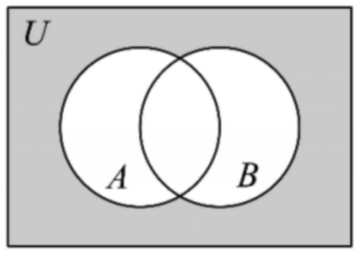
\includegraphics[width=0.20\textwidth]{figures/gao84_q9_venn.png}
\end{center}

\ifanswer
\solbegin
\step{$U=\{1,2,3,4,5,6,7,8,9,10\}$，$A=\{1,2\}$，$B=\{2,4\}$.}
\step{图中阴影部分表示的集合为 $\overline{A\cup B}=\{3,5,6,7,8,9,10\}$，共 $7$ 个元素，}
\step{其非空真子集的个数为 $2^7-2=126$.}
\solend
\fi

\item 若不等式 $ax^2-5x+c<0$ 的解集是 $(2,3)$，则不等式 $cx^2+5x+a\geqslant0$ 的解集是\blankline[4.4em].

\ifanswer
\solbegin
\step{若不等式 $ax^2-5x+c<0$ 的解集是 $(2,3)$，则 $a>0$ 且 $\begin{cases}\dfrac5a=5\\[2pt] \dfrac ca=6\end{cases}$，}
\step{则 $a=1$，$c=6$，}
\step{则不等式 $cx^2+5x+a\geqslant0$ 可化为 $6x^2+5x+1\geqslant0$，则 $x\leqslant-\dfrac12$ 或 $x\geqslant-\dfrac13$，}
\step{则不等式的解集为 $\left(-\infty,-\dfrac12\right]\cup\left[-\dfrac13,+\infty\right)$.}
\solend
\fi

\item 若关于 $x$ 的方程 $mx^2+2x+2=0$ 至少有一个负实根，则实数 $m$ 的取值范围是\blankline[4.4em].

\ifanswer
\solbegin
\step{①当 $m=0$ 时，方程为 $2x+2=0$，有一个负根，满足题意，}
\step{②当 $m\neq0$ 时，关于 $x$ 的方程 $mx^2+2x+2=0$ 至少有一个负根，}
\step{设根为 $x_1$、$x_2$，}
\step{当 $\Delta=4-8m=0$ 时，即 $m=\dfrac12$ 时，方程为 $\dfrac12x^2+2x+1=0$，}
\step{解得 $x=-2$，满足题意，}
\step{当 $\Delta=4-8m>0$，即 $m<\dfrac12$ 时，且 $m\neq0$ 时，}
\step{若有一个负根，则 $x_1x_2=\dfrac2m<0$，解得 $m<0$，}
\step{若有两个负根，则 $\begin{cases}x_1+x_2=-\dfrac2m<0\\[2pt] x_1x_2=\dfrac2m>0\end{cases}$，解得 $0<m<\dfrac12$，}
\step{综上所述，则实数 $m$ 的取值范围是 $\left(-\infty,\dfrac12\right]$.}
\solend
\fi

\item 设集合 $S$、$T$ 都至少含有两个元素，且 $S$、$T$ 同时满足：条件 1：对任意 $x$、$y\in S$，若
$x\neq y$，则 $x+y\in T$；条件 2：对任意 $x$、$y\in T$，若 $x\neq y$，则 $x-y\in S$. 给出下列说法：

①若 $S$ 只有 $2$ 个元素，则这 $2$ 个元素互为相反数；

②若 $S$ 只有 $2$ 个元素，则 $S\cup T$ 必有 $3$ 个元素；

③若 $S$ 只有 $2$ 个元素，则 $S\cup T$ 可能有 $4$ 个元素；

④存在含有 $3$ 个元素的集合 $S$，满足 $S\cup T$ 有 $4$ 个元素.

其中所有正确说法的序号是\blankline[4.4em].

\ifanswer
\solbegin
\step{对于①：由条件 2 得 $x-y\in S$，$y-x\in S$，且 $x-y\neq y-x$，}
\step{所以若 $S$ 只有 $2$ 个元素，则这 $2$ 个元素互为相反数，故①正确；}
\step{对于④：若 $S$ 有 $3$ 个元素，不妨设 $S=\{a,b,c\}$，其中 $a<b<c$，}
\step{则 $\{a+b,b+c,c+a\}\subseteq T$，所以 $c-a$、$c-b$、$b-a$、$a-c$、$b-c$、$a-b\in S$，}
\step{而 $c-a$ 与 $c-b$ 为两个互不相等的正数，$a-c$ 与 $a-b$ 为两个互不相等的负数，}
\step{故集合 $S$ 中至少有 $4$ 个元素，与 $S=\{a,b,c\}$ 有 $3$ 个元素矛盾，故④错误.}
\step{对于②③：若 $S$ 有 $2$ 个元素，由①得集合 $S$ 中的 $2$ 个元素必为相反数，}
\step{故可设 $S=\{a,-a\}(a\neq0)$. 由条件 1 得 $0\in T$，}
\step{由于集合 $T$ 中至少有 $2$ 个元素，故至少还有另外一个元素 $m\in T$.}
\step{当集合 $T$ 只有 $2$ 个元素时即 $T=\{0,m\}$，由条件 1 得 $-m\in S$，则 $m=\pm a$，}
\step{$T=\{0,a\}$ 或 $T=\{0,-a\}$，故 $S\cup T=\{0,a,-a\}$.}
\step{当集合 $T$ 有多于 $2$ 个元素时，不妨设 $T=\{0,m,n\}$，}
\step{则 $m$、$n$、$-m$、$-n$、$m-n$、$n-m\in S$，由于 $m$、$n\neq0$，}
\step{所以 $m\neq m-n$，$n\neq n-m$，又 $m\neq n$，}
\step{故集合 $S$ 至少有 $3$ 个元素，与 $S$ 中只有两个元素矛盾.}
\step{综上，$S\cup T=\{0,a,-a\}$，故②正确，③错误.}
\step{故正确的是①②.}
\solend
\fi

\end{enumerate}

\bigsec{二、选择题}

\begin{enumerate}
\setcounter{enumi}{12}

\item 用反证法证明命题：“若 $x+y>2$，则 $x>1$ 或 $y>1$”时，应假设\mbox{（\quad）}

\keepwithprev
A. $x\leqslant1$ 或 $y\leqslant1$\qquad B. 若 $x>1$ 或 $y>1$

C. $x\leqslant1$ 且 $y\leqslant1$\qquad D. 若 $x>1$ 且 $y>1$

\ifanswer
\ans{$C$}
\fi

\item 下列命题中，为真命题的是\mbox{（\quad）}

\keepwithprev
A. 若 $a>b$，则 $a^2>b^2$\qquad B. 若 $a>b$，$c>d$，则 $ac>bd$

C. 若 $a>b$，则 $\dfrac1a<\dfrac1b$\qquad D. 若 $ac^2>bc^2$，则 $a>b$

\ifanswer
\solbegin
\step{对于 $A$，当 $a=-1$，$b=-2$ 时，$a^2<b^2$，故 $A$ 错误；}
\step{对于 $B$，当 $a=-1$，$b=-2$，$c=-1$，$d=-2$ 时，$ac<bd$，故 $B$ 错误；}
\step{对于 $C$，当 $a=1$，$b=-2$ 时，$\dfrac1a>\dfrac1b$，故 $C$ 错误；}
\step{对于 $D$，因为 $ac^2-bc^2=(a-b)c^2>0$，所以 $a-b>0$，$c^2>0$，则 $a>b$，}
\step{故 $D$ 正确.}
\step{故选 $D$.}
\solend
\fi

\item 现有一级小麦 $m\,\mathrm{kg}$，二级小麦 $n\,\mathrm{kg}$，某粮食收购站有两种收购方案. 方案一：分两个
等级收购小麦，一级小麦 $a$ 元$/\mathrm{kg}$，二级小麦 $b$ 元$/\mathrm{kg}\,(b<a)$；方案二：以方案一两种价
格的平均数收购. 收购方式更加优惠的是\mbox{（\quad）}

\keepwithprev
A. 方案一\qquad B. 方案二\qquad C. 同样优惠\qquad D. 以上均有可能

\ifanswer
\solbegin
\step{方案一收购的平均价格为 $\dfrac{ma+nb}{m+n}$，方案二收购的平均价格为 $\dfrac{a+b}2$；}
\step{所以 $\dfrac{ma+nb}{m+n}-\dfrac{a+b}2=\dfrac{(a-b)(m-n)}{2(m+n)}$ ①，}
\step{$a-b>0$，$m-n$ 的正负性不确定，故①式的正负性不确定，故选 $D$.}
\solend
\fi

\item 用 $C(A)$ 表示非空集合 $A$ 中的元素个数. 对于集合 $A$、$B$，定义

$A*B=\begin{cases}C(A)-C(B),&C(A)\geqslant C(B)\\ C(B)-C(A),&C(A)<C(B)\end{cases}$，若 $A=\{0,1\}$，

$B=\{x\mid(x^2-ax)(x^2+ax+2)=0\}$，设实数 $a$ 的所有可能取值组成的集合是 $S$，则下列选
项不正确的是\mbox{（\quad）}

\keepwithprev
A. $C(B)$ 的可能值为 $1$，$2$，$3$，$4$

B. 若 $A*B=2$，则 $a$ 的取值范围为 $(-\infty,-2\sqrt2)\cup(2\sqrt2,+\infty)$

C. 若 $A*B=1$，则 $C(S)=3$

D. 若 $A*B=0$，则 $a$ 的取值范围为 $(-2\sqrt2,2\sqrt2)$

\ifanswer
\solbegin
\step{对于集合 $B$，当 $a=0$ 时，方程 $x^2(x^2+2)=0$ 的解为 $x=0$，$C(B)=1$，}
\step{当 $a\neq0$ 时，$x^2-ax=0$ 或 $x^2+ax+2=0$，}
\step{其中 $x^2-ax=0$ 的解为 $x_1=0$，$x_2=a$，}
\step{若 $\Delta=a^2-8>0$，即 $a>2\sqrt2$ 或 $a<-2\sqrt2$，}
\step{方程 $x^2+ax+2=0$ 有两个不相等的实数根，此时 $C(B)=4$；}
\step{若 $\Delta=a^2-8=0$，即 $a=2\sqrt2$ 或 $-2\sqrt2$，}
\step{方程 $x^2+ax+2=0$ 有两个相等的实数根，此时 $C(B)=3$；}
\step{若 $\Delta=a^2-8<0$，即 $-2\sqrt2<a<0$ 或 $0<a<2\sqrt2$，}
\step{方程 $x^2+ax+2=0$ 无实数根，此时 $C(B)=2$；}
\step{所以 $C(B)$ 的可能值为 $1$，$2$，$3$，$4$，故 $A$ 正确；}
\step{若 $A*B=2$，且 $C(A)=2$，则 $C(B)=4$，}
\step{则 $a$ 的取值范围 $(-\infty,-2\sqrt2)\cup(2\sqrt2,+\infty)$，故 $B$ 正确；}
\step{若 $A*B=1$，且 $C(A)=2$，则 $C(B)=1$ 或 $3$，}
\step{当 $C(B)=1$ 时，$a=0$，}
\step{当 $C(B)=3$ 时，$a=2\sqrt2$ 或 $-2\sqrt2$，此时集合 $S=\{0,-2\sqrt2,2\sqrt2\}$，}
\step{则 $C(S)=3$，故 $C$ 正确；}
\step{若 $A*B=0$，且 $C(A)=2$，则 $C(B)=2$，}
\step{由此可得 $a$ 的取值范围为 $(-2\sqrt2,0)\cup(0,2\sqrt2)$，故 $D$ 不正确；}
\step{故选 $D$.}
\solend
\fi

\end{enumerate}

\bigsec{三、解答题}

\begin{enumerate}
\setcounter{enumi}{16}

\item 已知集合 $A=\{x\mid-3<x\leqslant4\}$，集合 $B=\{x\mid k+1\leqslant x\leqslant2k-1\}$.

（1）当 $k=3$ 时，求 $A\cup B$、$\overline A\cap B$；

（2）若 $B\subseteq A$，求 $k$ 的取值范围.

\ansspace*[10]

\ifanswer
\solbegin
\stepm{（1）}{当 $k=3$ 时，$B=\{x\mid4\leqslant x\leqslant5\}$，又 $A=\{x\mid-3<x\leqslant4\}$，}
\step{所以 $\overline A=\{x\mid x\leqslant-3$ 或 $x>4\}$，}
\step{所以 $A\cup B=\{x\mid-3<x\leqslant5\}$，$\overline A\cap B=\{x\mid4<x\leqslant5\}$.}
\stepm{（2）}{①当 $B=\varnothing$，即 $k+1>2k-1$ 时，$k<2$，满足 $B\subseteq A$.}
\step{②当 $B\neq\varnothing$ 时，由 $B\subseteq A$ 得 $\begin{cases}k+1\leqslant2k-1\\ k+1>-3\\ 2k-1\leqslant4\end{cases}$，解得 $2\leqslant k\leqslant\dfrac52$，}
\step{综合①②得 $k$ 的取值范围 $\left\{k\mid k\leqslant\dfrac52\right\}$.}
\solend
\fi

\item 设集合 $A=\{x\mid x^2-3x+2=0\}$，$B=\{x\mid x^2+2(a+1)x+a^2-5=0\}$.

（1）若 $A\cap B=\{2\}$，求实数 $a$ 的值；

（2）若集合 $B$ 中有两个元素 $x_1,x_2$，求 $\lvert x_1-x_2\rvert$（用 $a$ 表示）.

\ansspace*[10]

\ifanswer
\solbegin
\stepm{（1）}{由题意得 $A=\{x\mid x^2-3x+2=0\}=\{1,2\}$，因为 $A\cap B=\{2\}$，所以 $2\in B$，}
\step{所以 $2^2+4(a+1)+a^2-5=0$ 即 $4+4a+4+a^2-5=0$，}
\step{化简得 $a^2+4a+3=0$，即 $(a+3)(a+1)=0$，解得 $a=-3$ 或 $a=-1$，}
\step{检验：当 $a=-3$ 时，$B=\{x\mid x^2-4x+4=0\}=\{2\}$，满足 $A\cap B=\{2\}$，}
\step{当 $a=-1$ 时，$B=\{x\mid x^2-4=0\}=\{-2,2\}$，满足 $A\cap B=\{2\}$，}
\step{所以 $a=-3$ 或 $a=-1$.}
\stepm{（2）}{因为 $B$ 中有两个元素 $x_1,x_2$，所以 $x^2+2(a+1)x+(a^2-5)=0$ 有两个根，}
\step{所以 $\Delta=4(a+1)^2-4(a^2-5)=8a+24>0$，}
\step{且 $x_1+x_2=-2(a+1)$，$x_1x_2=a^2-5$，}
\step{所以 $\lvert x_1-x_2\rvert=\sqrt{(x_1+x_2)^2-4x_1x_2}=\sqrt{4(a+1)^2-4(a^2-5)}=\sqrt{8a+24}$.}
\solend
\fi

\item 已知关于 $x$ 的不等式 $\dfrac{ax-2}{1+x}>0$.

（1）若 $x=-a$ 时，不等式成立，求实数 $a$ 的取值范围；

（2）若 $a$ 为实数，解关于 $x$ 的不等式：$\dfrac{ax-2}{1+x}>0$.

\ansspace*[12]

\ifanswer
\solbegin
\stepm{（1）}{因为 $x=-a$ 时，不等式成立，}
\step{所以 $\dfrac{-a^2-2}{1-a}>0\Rightarrow\dfrac{a^2+2}{a-1}>0\Rightarrow a-1>0\Rightarrow a>1$，}
\step{所以实数 $a$ 的取值范围为 $(1,+\infty)$.}
\stepm{（2）}{$\dfrac{ax-2}{1+x}>0\Rightarrow(ax-2)(x+1)>0$，}
\step{当 $a=0$ 时，$-2(x+1)>0$，解得 $x<-1$.}
\step{当 $a>0$ 时，$(ax-2)(x+1)>0$，解得 $x>\dfrac2a$ 或 $x<-1$.}
\step{当 $a<0$ 时，不等式 $(ax-2)(x+1)>0$ 可化为 $\left(x-\dfrac2a\right)(x+1)<0$，}
\step{当 $\dfrac2a>-1$，即 $a<-2$ 时，解得 $-1<x<\dfrac2a$；}
\step{当 $\dfrac2a<-1$，即 $-2<a<0$ 时，解得 $\dfrac2a<x<-1$；}
\step{当 $\dfrac2a=-1$，即 $a=-2$ 时，解集为 $\varnothing$.}
\step{综上，当 $a<-2$ 时，不等式的解集为 $\left(-1,\dfrac2a\right)$；}
\step{当 $a=-2$ 时，不等式的解集为 $\varnothing$；}
\step{当 $-2<a<0$ 时，不等式的解集为 $\left(\dfrac2a,-1\right)$；}
\step{当 $a=0$ 时，不等式的解集为 $(-\infty,-1)$；}
\step{当 $a>0$ 时，不等式的解集为 $(-\infty,-1)\cup\left(\dfrac2a,+\infty\right)$.}
\solend
\fi

\item 已知关于 $x$ 的不等式 $(k^2-2k-3)x^2+(k+1)x+1>0\,(k\in\R)$ 的解集为 $M$；

（1）若存在实数 $a$，使得 $M=(-\infty,a)\cup(a,+\infty)$，求 $k$ 的值；

（2）若 $M=\R$，求 $k$ 的取值范围；

（3）是否存在实数 $k$，满足：“对于任意 $n\in\N$，$n>0$，都有 $n\in M$；对于任意
$m\in\Z$，$m<0$，都有 $m\notin M$”，若存在，求出 $k$ 的值，若不存在，说明理由.

\ansspace*[13]

\ifanswer
\solbegin
\stepm{（1）}{记 $f(x)=(k^2-2k-3)x^2+(k+1)x+1$.}
\step{$M=(-\infty,a)\cup(a,+\infty)$ 表示 $f(x)>0$ 对一切 $x\neq a$ 成立，且 $f(a)=0$，}
\step{故需二次项系数大于 $0$ 且 $\Delta=0$.}
\step{由 $\Delta=(k+1)^2-4(k^2-2k-3)=-3k^2+10k+13=0$ 得 $k=\dfrac{13}3$ 或 $k=-1$.}
\step{当 $k=\dfrac{13}3$ 时，二次项系数 $\dfrac{64}9>0$，$f(x)=\dfrac{64}9\left(x+\dfrac38\right)^2$，符合；}
\step{当 $k=-1$ 时二次项系数为 $0$，$f(x)=1>0$，$M=\R$，不符合. 故 $k=\dfrac{13}3$.}
\stepm{（2）}{$M=\R$ 即 $f(x)>0$ 对一切 $x\in\R$ 恒成立.}
\step{①当 $k^2-2k-3>0$（即 $k<-1$ 或 $k>3$）时，需 $\Delta<0$，}
\step{即 $-3k^2+10k+13<0$，得 $k<-1$ 或 $k>\dfrac{13}3$，故 $k<-1$ 或 $k>\dfrac{13}3$；}
\step{②当 $k^2-2k-3=0$ 时，$k=3$ 得 $f(x)=4x+1$ 不恒正，不符合题意，}
\step{舍去，}
\step{当 $k=-1$ 得 $f(x)=1>0$ 恒成立，符合题意；}
\step{③当 $k^2-2k-3<0$ 时，抛物线开口向下，不能恒正.}
\step{综上，$k\leqslant-1$ 或 $k>\dfrac{13}3$.}
\stepm{（3）}{存在，$k=3$，理由如下，}
\step{由题意得解集 $M=(t,+\infty)$，$t\in[-1,1)$；}
\step{当 $k^2-2k-3=0$ 时，解得 $k=3$ 或 $k=-1$，}
\step{$k=3$ 时，不等式的解集为 $\left(-\dfrac14,+\infty\right)$，满足条件；}
\step{$k=-1$ 时，$1>0$ 恒成立，不满足条件；}
\step{当 $k^2-2k-3>0$ 时，}
\step{此时对应的一元二次不等式的解集形式不是 $(t,+\infty)$ 的形式，不满足条件；}
\step{当 $k^2-2k-3<0$ 时，}
\step{此时对应的一元二次不等式的解集形式不是 $(t,+\infty)$ 的形式，不满足条件；}
\step{综上，满足条件 $k$ 的值为 $3$.}
\solend
\fi

\item 已知有限集 $A=\{a_1,a_2,\cdots,a_n\}\,(n\geqslant2,n\in\N)$，如果 $A$ 中元素 $a_i\,(i=1,2,3,\cdots,n)$ 满足
$a_1+a_2+a_3+\cdots+a_n=a_1\times a_2\times\cdots\times a_n$，就称 $A$ 为“和积平衡集”.

（1）判断集合 $\{-1+\sqrt3,-1-\sqrt3\}$ 是否为“和积平衡集”；

（2）若 $a_1$、$a_2$ 是两个不同的正数，且 $\{a_1,a_2\}$ 是“和积平衡集”，写出以 $a_1$、$a_2$ 为根的一
个一元二次方程（系数可用 $a_1$、$a_2$ 表示），并证明 $a_1$、$a_2$ 至少有一个大于 $2$；

（3）若 $a_i\in\Z$ 且 $a_i>0$，求所有符合条件的“和积平衡集”.

\ansspace*[14]

\ifanswer
\solbegin
\stepm{（1）}{对于集合 $\{-1+\sqrt3,-1-\sqrt3\}$，}
\step{因为 $(-1+\sqrt3)+(-1-\sqrt3)=-2$，$(-1+\sqrt3)\times(-1-\sqrt3)=-2$，}
\step{所以满足 $a_1+a_2=a_1\times a_2$，满足题意，}
\step{所以集合 $\{-1+\sqrt3,-1-\sqrt3\}$ 是和积平衡集.}
\stepm{（2）}{以 $a_1$、$a_2$ 为根的一个一元二次方程可为 $x^2-(a_1+a_2)x+a_1\cdot a_2=0$，}
\step{因为 $a_1$、$a_2$ 是两个不同的正数，且 $\{a_1,a_2\}$ 是和积平衡集，}
\step{所以 $a_1+a_2=a_1\cdot a_2$，}
\step{又 $a_1$ 和 $a_2$ 为 $x^2-(a_1+a_2)x+a_1\cdot a_2=0$ 的两个不同的正根，}
\step{所以 $\Delta=(a_1+a_2)^2-4a_1a_2=(a_1+a_2)^2-4(a_1+a_2)>0$，}
\step{又 $a_1+a_2>0$，则 $a_1+a_2>4$，}
\step{若 $a_1$、$a_2$ 都小于等于 $2$，则 $a_1+a_2\leqslant4$，矛盾，}
\step{所以 $a_1$、$a_2$ 至少有一个大于 $2$；}
\stepm{（3）}{设 $A$ 中的 $a_1<a_2<a_3<\cdots<a_n$，且 $a_i\in\N^*$，}
\step{由 $a_1+a_2+a_3+\cdots+a_n=a_1\times a_2\times\cdots\times a_n$，得 $n=2$ 时明显不满足，}
\step{所以 $n\geqslant3$，故 $a_1\times a_2\times\cdots\times a_n=a_1+a_2+a_3+\cdots+a_n\leqslant na_n$，}
\step{所以 $a_1\times a_2\times\cdots\times a_{n-1}\leqslant n$，}
\step{当 $n=3$ 时，$a_1\times a_2\leqslant3$，$a_i\in\N^*$，只能有 $a_1=1$，$a_2=2$，}
\step{由 $a_1+a_2+a_3=a_1\times a_2\times a_3$，得 $a_3=3$，此时的和积平衡集为 $\{1,2,3\}$，}
\step{当 $n\geqslant4$ 时，$a_1\times a_2\times\cdots\times a_{n-1}\geqslant(n-1)(n-2)\times\cdots\times2\times1\geqslant(n-1)(n-2)$，}
\step{又 $(n-1)(n-2)-n=n^2-4n+2=n(n-4)+2>0$，即 $(n-1)(n-2)>n$，}
\step{即 $a_1\times a_2\times\cdots\times a_{n-1}>n$，与 $a_1\times a_2\times\cdots\times a_{n-1}\leqslant n$ 矛盾，}
\step{所以 $n\geqslant4$ 不满足条件，}
\step{所以符合条件的和积平衡集有且只有 $n=3$，此时的和积平衡集为 $\{1,2,3\}$.}
\solend
\fi

\end{enumerate}

\end{document}
"
%
% 原始材料：微信公众号“魔都数学加油站”文章，连载“27学年高一84”；
% 原文标题“27学年高一84——2026-2027年上海市东昌中学高一上10月月考”；
% 原文链接：https://mp.weixin.qq.com/s/PErsjO3N5RsMuJC69IGbrw。
% 页面标注发布时间 2026-10-26 20:15（上海）。
% 正文为 12 张 PNG 页（`原图/高一84_东昌中学_10月月考/01..12.png`），
% 尺寸混排（第 1—8 页为 4762×6735，第 9—12 页为 2560×3620），均按页序读取。
%
% 篇幅与题号：原卷自第 3 题起编号（第 1、2 题不在原文内）。填空题 3—12（10 题）、
% 选择题 13—16（4 题）、解答题 17—21（5 题），共 19 题。
%
% 讲评版：19 题全部印【解析】，本稿不另提 \ans{}；选择题答案在解析末句“故选 D／C／D”。
% 第 13 题的答案“C”原卷直接印在题干括号内（“（\ C\ ）”），本稿按 高一37 第 13 题／
% 高一63 第 14 题成例括号留空、另提 \ans{$C$}（该题无【解析】段）。
%
% 副标题：原卷未印副标题。本稿按内容标作“集合与常用逻辑用语、不等式”。
%
% 与原卷的排版差异：
%   ① 原卷每题下直接印【解析】，本稿按全稿惯例将解析置于答案版；
%   ② 原卷未印副标题，本稿补出；填空横线统一排 \blankline[4.4em]；
%   ③ 原卷数集记号排斜体 $R$、$Z$、$N$，本稿按全稿惯例改用 $\R$、$\Z$、$\N$；
%   ④ 第 17—21 题的子问用行内“（1）（2）（3）”段，解析中的子问标号用 \stepm；
%   ⑤ 解答题按惯例加 \ansspace；选择题括号排 \mbox{（\quad）}；
%   ⑥ 第 9 题题干右侧有一幅韦恩图，裁自原图（第 2 页）后去粉色水印、转灰度，
%      三版都出（属题干）。
%
% 行数核对：逐题数 \step/\stepm 条数，合计 157 条（Q3：2；Q4：2；Q5：3；Q6：2；
% Q7：3；Q8：6；Q9：3；Q10：4；Q11：9；Q12：17；Q14：6；Q15：3；Q16：19；
% Q17：6；Q18：10；Q19：15；Q20：24；Q21：23）；第 13 题无解析，只提 \ans{}，
% 不计入 \step 账。原卷解析的换行按语意合并，未逐行强拆。
%
\documentclass[a4paper,11pt]{article}
\usepackage{common}

\begin{document}

\examtitlest[4]{2026--2027 年东昌中学高一上 10 月月考}{集合与常用逻辑用语、不等式}

\bigsec{一、填空题}

\begin{enumerate}
\setcounter{enumi}{2}

\item 若 $a\in\R$，则“$a=2$”是“$(a-1)(a-2)=0$”的\blankline[3.6em]条件（填“充分不必要”、“必要
不充分”、“充要”、“既不充分又不必要”的一个）.

\ifanswer
\solbegin
\step{$a=2\Rightarrow(a-1)(a-2)=0$，而 $(a-1)(a-2)=0$ 不能推出 $a=2$，}
\step{故“$a=2$”是“$(a-1)(a-2)=0$”的充分不必要条件.}
\solend
\fi

\item 已知集合 $M=\{(x,y)\mid y=x^2\}$，$N=\{(x,y)\mid y=1\}$，则 $M\cap N=\blankline[4.4em]$.

\ifanswer
\solbegin
\step{集合 $M=\{(x,y)\mid y=x^2\}$，$N=\{(x,y)\mid y=1\}$，}
\step{当 $y=1$ 时，$x=\pm1$，则 $M\cap N=\{(-1,1),(1,1)\}$.}
\solend
\fi

\item 已知集合 $A=\{x\mid x^2+ax+4=0\}$，若 $A$ 有且只有一个非空子集，则实数 $a=\blankline[4.4em]$.

\ifanswer
\solbegin
\step{因为集合 $A$ 有且只有一个非空子集，所以集合 $A$ 中只有一个元素，}
\step{所以一元二次方程 $x^2+ax+4=0$ 有两个相等的解，}
\step{所以 $\Delta=a^2-4\times4=0$，解得 $a=\pm4$.}
\solend
\fi

\item 已知 $A=(-\infty,a]$，$B=(-\infty,3)$，且 $x\in A$ 是 $x\in B$ 的充分不必要条件，则 $a$ 的取值范围
是\blankline[4.4em].

\ifanswer
\solbegin
\step{$A=(-\infty,a]$，$B=(-\infty,3)$，且 $x\in A$ 是 $x\in B$ 的充分不必要条件，}
\step{则 $A\subset B$，则 $a<3$，即 $a$ 的取值范围为 $(-\infty,3)$.}
\solend
\fi

\item 不等式 $\dfrac{3x-1}{x-2}\leqslant1$ 的解集为\blankline[4.4em].

\ifanswer
\solbegin
\step{由 $\dfrac{3x-1}{x-2}\leqslant1$，得 $\dfrac{3x-1}{x-2}-1=\dfrac{3x-1-(x-2)}{x-2}=\dfrac{2x+1}{x-2}\leqslant0$，}
\step{则 $\begin{cases}(2x+1)(x-2)\leqslant0\\ x-2\neq0\end{cases}$，解得 $-\dfrac12\leqslant x<2$，}
\step{则不等式 $\dfrac{3x-1}{x-2}\leqslant1$ 的解集为 $\left[-\dfrac12,2\right)$.}
\solend
\fi

\item 已知关于 $x$ 的一元二次方程 $x^2-2mx+(3m+1)=0$ 的两个实数根为 $x_1$、$x_2$，且
$x_1^2+x_2^2=16$，则实数 $m$ 的值为\blankline[4.4em].

\ifanswer
\solbegin
\step{由韦达定理，得 $x_1+x_2=2m$，$x_1x_2=3m+1$，}
\step{$x_1^2+x_2^2=(x_1+x_2)^2-2x_1x_2=4m^2-6m-2$，}
\step{由 $x_1^2+x_2^2=16$，得 $4m^2-6m-2=16$，即 $2m^2-3m-9=0$，}
\step{解得 $m=3$ 或 $m=-\dfrac32$，}
\step{检验判别式 $\Delta=4m^2-12m-4$，当 $m=3$ 时，$\Delta=-4<0$，舍去；}
\step{当 $m=-\dfrac32$ 时，$\Delta=23>0$，符合条件，故 $m=-\dfrac32$.}
\solend
\fi

\item 已知全集 $U=\{x\mid1\leqslant x\leqslant10,\,x\in\N\}$，集合 $A=\{x\mid x^2-3<4,\,x\in\N,\,x>0\}$，
$B=\{2,4\}$，则图中阴影部分表示的集合的非空真子集个数为\blankline[4.4em].

\needvspace{9\baselineskip}
\begin{center}
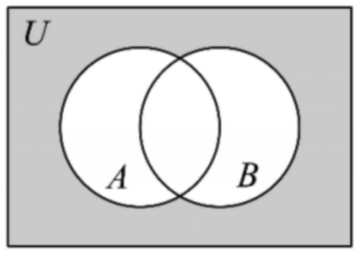
\includegraphics[width=0.20\textwidth]{figures/gao84_q9_venn.png}
\end{center}

\ifanswer
\solbegin
\step{$U=\{1,2,3,4,5,6,7,8,9,10\}$，$A=\{1,2\}$，$B=\{2,4\}$.}
\step{图中阴影部分表示的集合为 $\overline{A\cup B}=\{3,5,6,7,8,9,10\}$，共 $7$ 个元素，}
\step{其非空真子集的个数为 $2^7-2=126$.}
\solend
\fi

\item 若不等式 $ax^2-5x+c<0$ 的解集是 $(2,3)$，则不等式 $cx^2+5x+a\geqslant0$ 的解集是\blankline[4.4em].

\ifanswer
\solbegin
\step{若不等式 $ax^2-5x+c<0$ 的解集是 $(2,3)$，则 $a>0$ 且 $\begin{cases}\dfrac5a=5\\[2pt] \dfrac ca=6\end{cases}$，}
\step{则 $a=1$，$c=6$，}
\step{则不等式 $cx^2+5x+a\geqslant0$ 可化为 $6x^2+5x+1\geqslant0$，则 $x\leqslant-\dfrac12$ 或 $x\geqslant-\dfrac13$，}
\step{则不等式的解集为 $\left(-\infty,-\dfrac12\right]\cup\left[-\dfrac13,+\infty\right)$.}
\solend
\fi

\item 若关于 $x$ 的方程 $mx^2+2x+2=0$ 至少有一个负实根，则实数 $m$ 的取值范围是\blankline[4.4em].

\ifanswer
\solbegin
\step{①当 $m=0$ 时，方程为 $2x+2=0$，有一个负根，满足题意，}
\step{②当 $m\neq0$ 时，关于 $x$ 的方程 $mx^2+2x+2=0$ 至少有一个负根，}
\step{设根为 $x_1$、$x_2$，}
\step{当 $\Delta=4-8m=0$ 时，即 $m=\dfrac12$ 时，方程为 $\dfrac12x^2+2x+1=0$，}
\step{解得 $x=-2$，满足题意，}
\step{当 $\Delta=4-8m>0$，即 $m<\dfrac12$ 时，且 $m\neq0$ 时，}
\step{若有一个负根，则 $x_1x_2=\dfrac2m<0$，解得 $m<0$，}
\step{若有两个负根，则 $\begin{cases}x_1+x_2=-\dfrac2m<0\\[2pt] x_1x_2=\dfrac2m>0\end{cases}$，解得 $0<m<\dfrac12$，}
\step{综上所述，则实数 $m$ 的取值范围是 $\left(-\infty,\dfrac12\right]$.}
\solend
\fi

\item 设集合 $S$、$T$ 都至少含有两个元素，且 $S$、$T$ 同时满足：条件 1：对任意 $x$、$y\in S$，若
$x\neq y$，则 $x+y\in T$；条件 2：对任意 $x$、$y\in T$，若 $x\neq y$，则 $x-y\in S$. 给出下列说法：

①若 $S$ 只有 $2$ 个元素，则这 $2$ 个元素互为相反数；

②若 $S$ 只有 $2$ 个元素，则 $S\cup T$ 必有 $3$ 个元素；

③若 $S$ 只有 $2$ 个元素，则 $S\cup T$ 可能有 $4$ 个元素；

④存在含有 $3$ 个元素的集合 $S$，满足 $S\cup T$ 有 $4$ 个元素.

其中所有正确说法的序号是\blankline[4.4em].

\ifanswer
\solbegin
\step{对于①：由条件 2 得 $x-y\in S$，$y-x\in S$，且 $x-y\neq y-x$，}
\step{所以若 $S$ 只有 $2$ 个元素，则这 $2$ 个元素互为相反数，故①正确；}
\step{对于④：若 $S$ 有 $3$ 个元素，不妨设 $S=\{a,b,c\}$，其中 $a<b<c$，}
\step{则 $\{a+b,b+c,c+a\}\subseteq T$，所以 $c-a$、$c-b$、$b-a$、$a-c$、$b-c$、$a-b\in S$，}
\step{而 $c-a$ 与 $c-b$ 为两个互不相等的正数，$a-c$ 与 $a-b$ 为两个互不相等的负数，}
\step{故集合 $S$ 中至少有 $4$ 个元素，与 $S=\{a,b,c\}$ 有 $3$ 个元素矛盾，故④错误.}
\step{对于②③：若 $S$ 有 $2$ 个元素，由①得集合 $S$ 中的 $2$ 个元素必为相反数，}
\step{故可设 $S=\{a,-a\}(a\neq0)$. 由条件 1 得 $0\in T$，}
\step{由于集合 $T$ 中至少有 $2$ 个元素，故至少还有另外一个元素 $m\in T$.}
\step{当集合 $T$ 只有 $2$ 个元素时即 $T=\{0,m\}$，由条件 1 得 $-m\in S$，则 $m=\pm a$，}
\step{$T=\{0,a\}$ 或 $T=\{0,-a\}$，故 $S\cup T=\{0,a,-a\}$.}
\step{当集合 $T$ 有多于 $2$ 个元素时，不妨设 $T=\{0,m,n\}$，}
\step{则 $m$、$n$、$-m$、$-n$、$m-n$、$n-m\in S$，由于 $m$、$n\neq0$，}
\step{所以 $m\neq m-n$，$n\neq n-m$，又 $m\neq n$，}
\step{故集合 $S$ 至少有 $3$ 个元素，与 $S$ 中只有两个元素矛盾.}
\step{综上，$S\cup T=\{0,a,-a\}$，故②正确，③错误.}
\step{故正确的是①②.}
\solend
\fi

\end{enumerate}

\bigsec{二、选择题}

\begin{enumerate}
\setcounter{enumi}{12}

\item 用反证法证明命题：“若 $x+y>2$，则 $x>1$ 或 $y>1$”时，应假设\mbox{（\quad）}

\keepwithprev
A. $x\leqslant1$ 或 $y\leqslant1$\qquad B. 若 $x>1$ 或 $y>1$

C. $x\leqslant1$ 且 $y\leqslant1$\qquad D. 若 $x>1$ 且 $y>1$

\ifanswer
\ans{$C$}
\fi

\item 下列命题中，为真命题的是\mbox{（\quad）}

\keepwithprev
A. 若 $a>b$，则 $a^2>b^2$\qquad B. 若 $a>b$，$c>d$，则 $ac>bd$

C. 若 $a>b$，则 $\dfrac1a<\dfrac1b$\qquad D. 若 $ac^2>bc^2$，则 $a>b$

\ifanswer
\solbegin
\step{对于 $A$，当 $a=-1$，$b=-2$ 时，$a^2<b^2$，故 $A$ 错误；}
\step{对于 $B$，当 $a=-1$，$b=-2$，$c=-1$，$d=-2$ 时，$ac<bd$，故 $B$ 错误；}
\step{对于 $C$，当 $a=1$，$b=-2$ 时，$\dfrac1a>\dfrac1b$，故 $C$ 错误；}
\step{对于 $D$，因为 $ac^2-bc^2=(a-b)c^2>0$，所以 $a-b>0$，$c^2>0$，则 $a>b$，}
\step{故 $D$ 正确.}
\step{故选 $D$.}
\solend
\fi

\item 现有一级小麦 $m\,\mathrm{kg}$，二级小麦 $n\,\mathrm{kg}$，某粮食收购站有两种收购方案. 方案一：分两个
等级收购小麦，一级小麦 $a$ 元$/\mathrm{kg}$，二级小麦 $b$ 元$/\mathrm{kg}\,(b<a)$；方案二：以方案一两种价
格的平均数收购. 收购方式更加优惠的是\mbox{（\quad）}

\keepwithprev
A. 方案一\qquad B. 方案二\qquad C. 同样优惠\qquad D. 以上均有可能

\ifanswer
\solbegin
\step{方案一收购的平均价格为 $\dfrac{ma+nb}{m+n}$，方案二收购的平均价格为 $\dfrac{a+b}2$；}
\step{所以 $\dfrac{ma+nb}{m+n}-\dfrac{a+b}2=\dfrac{(a-b)(m-n)}{2(m+n)}$ ①，}
\step{$a-b>0$，$m-n$ 的正负性不确定，故①式的正负性不确定，故选 $D$.}
\solend
\fi

\item 用 $C(A)$ 表示非空集合 $A$ 中的元素个数. 对于集合 $A$、$B$，定义

$A*B=\begin{cases}C(A)-C(B),&C(A)\geqslant C(B)\\ C(B)-C(A),&C(A)<C(B)\end{cases}$，若 $A=\{0,1\}$，

$B=\{x\mid(x^2-ax)(x^2+ax+2)=0\}$，设实数 $a$ 的所有可能取值组成的集合是 $S$，则下列选
项不正确的是\mbox{（\quad）}

\keepwithprev
A. $C(B)$ 的可能值为 $1$，$2$，$3$，$4$

B. 若 $A*B=2$，则 $a$ 的取值范围为 $(-\infty,-2\sqrt2)\cup(2\sqrt2,+\infty)$

C. 若 $A*B=1$，则 $C(S)=3$

D. 若 $A*B=0$，则 $a$ 的取值范围为 $(-2\sqrt2,2\sqrt2)$

\ifanswer
\solbegin
\step{对于集合 $B$，当 $a=0$ 时，方程 $x^2(x^2+2)=0$ 的解为 $x=0$，$C(B)=1$，}
\step{当 $a\neq0$ 时，$x^2-ax=0$ 或 $x^2+ax+2=0$，}
\step{其中 $x^2-ax=0$ 的解为 $x_1=0$，$x_2=a$，}
\step{若 $\Delta=a^2-8>0$，即 $a>2\sqrt2$ 或 $a<-2\sqrt2$，}
\step{方程 $x^2+ax+2=0$ 有两个不相等的实数根，此时 $C(B)=4$；}
\step{若 $\Delta=a^2-8=0$，即 $a=2\sqrt2$ 或 $-2\sqrt2$，}
\step{方程 $x^2+ax+2=0$ 有两个相等的实数根，此时 $C(B)=3$；}
\step{若 $\Delta=a^2-8<0$，即 $-2\sqrt2<a<0$ 或 $0<a<2\sqrt2$，}
\step{方程 $x^2+ax+2=0$ 无实数根，此时 $C(B)=2$；}
\step{所以 $C(B)$ 的可能值为 $1$，$2$，$3$，$4$，故 $A$ 正确；}
\step{若 $A*B=2$，且 $C(A)=2$，则 $C(B)=4$，}
\step{则 $a$ 的取值范围 $(-\infty,-2\sqrt2)\cup(2\sqrt2,+\infty)$，故 $B$ 正确；}
\step{若 $A*B=1$，且 $C(A)=2$，则 $C(B)=1$ 或 $3$，}
\step{当 $C(B)=1$ 时，$a=0$，}
\step{当 $C(B)=3$ 时，$a=2\sqrt2$ 或 $-2\sqrt2$，此时集合 $S=\{0,-2\sqrt2,2\sqrt2\}$，}
\step{则 $C(S)=3$，故 $C$ 正确；}
\step{若 $A*B=0$，且 $C(A)=2$，则 $C(B)=2$，}
\step{由此可得 $a$ 的取值范围为 $(-2\sqrt2,0)\cup(0,2\sqrt2)$，故 $D$ 不正确；}
\step{故选 $D$.}
\solend
\fi

\end{enumerate}

\bigsec{三、解答题}

\begin{enumerate}
\setcounter{enumi}{16}

\item 已知集合 $A=\{x\mid-3<x\leqslant4\}$，集合 $B=\{x\mid k+1\leqslant x\leqslant2k-1\}$.

（1）当 $k=3$ 时，求 $A\cup B$、$\overline A\cap B$；

（2）若 $B\subseteq A$，求 $k$ 的取值范围.

\ansspace*[10]

\ifanswer
\solbegin
\stepm{（1）}{当 $k=3$ 时，$B=\{x\mid4\leqslant x\leqslant5\}$，又 $A=\{x\mid-3<x\leqslant4\}$，}
\step{所以 $\overline A=\{x\mid x\leqslant-3$ 或 $x>4\}$，}
\step{所以 $A\cup B=\{x\mid-3<x\leqslant5\}$，$\overline A\cap B=\{x\mid4<x\leqslant5\}$.}
\stepm{（2）}{①当 $B=\varnothing$，即 $k+1>2k-1$ 时，$k<2$，满足 $B\subseteq A$.}
\step{②当 $B\neq\varnothing$ 时，由 $B\subseteq A$ 得 $\begin{cases}k+1\leqslant2k-1\\ k+1>-3\\ 2k-1\leqslant4\end{cases}$，解得 $2\leqslant k\leqslant\dfrac52$，}
\step{综合①②得 $k$ 的取值范围 $\left\{k\mid k\leqslant\dfrac52\right\}$.}
\solend
\fi

\item 设集合 $A=\{x\mid x^2-3x+2=0\}$，$B=\{x\mid x^2+2(a+1)x+a^2-5=0\}$.

（1）若 $A\cap B=\{2\}$，求实数 $a$ 的值；

（2）若集合 $B$ 中有两个元素 $x_1,x_2$，求 $\lvert x_1-x_2\rvert$（用 $a$ 表示）.

\ansspace*[10]

\ifanswer
\solbegin
\stepm{（1）}{由题意得 $A=\{x\mid x^2-3x+2=0\}=\{1,2\}$，因为 $A\cap B=\{2\}$，所以 $2\in B$，}
\step{所以 $2^2+4(a+1)+a^2-5=0$ 即 $4+4a+4+a^2-5=0$，}
\step{化简得 $a^2+4a+3=0$，即 $(a+3)(a+1)=0$，解得 $a=-3$ 或 $a=-1$，}
\step{检验：当 $a=-3$ 时，$B=\{x\mid x^2-4x+4=0\}=\{2\}$，满足 $A\cap B=\{2\}$，}
\step{当 $a=-1$ 时，$B=\{x\mid x^2-4=0\}=\{-2,2\}$，满足 $A\cap B=\{2\}$，}
\step{所以 $a=-3$ 或 $a=-1$.}
\stepm{（2）}{因为 $B$ 中有两个元素 $x_1,x_2$，所以 $x^2+2(a+1)x+(a^2-5)=0$ 有两个根，}
\step{所以 $\Delta=4(a+1)^2-4(a^2-5)=8a+24>0$，}
\step{且 $x_1+x_2=-2(a+1)$，$x_1x_2=a^2-5$，}
\step{所以 $\lvert x_1-x_2\rvert=\sqrt{(x_1+x_2)^2-4x_1x_2}=\sqrt{4(a+1)^2-4(a^2-5)}=\sqrt{8a+24}$.}
\solend
\fi

\item 已知关于 $x$ 的不等式 $\dfrac{ax-2}{1+x}>0$.

（1）若 $x=-a$ 时，不等式成立，求实数 $a$ 的取值范围；

（2）若 $a$ 为实数，解关于 $x$ 的不等式：$\dfrac{ax-2}{1+x}>0$.

\ansspace*[12]

\ifanswer
\solbegin
\stepm{（1）}{因为 $x=-a$ 时，不等式成立，}
\step{所以 $\dfrac{-a^2-2}{1-a}>0\Rightarrow\dfrac{a^2+2}{a-1}>0\Rightarrow a-1>0\Rightarrow a>1$，}
\step{所以实数 $a$ 的取值范围为 $(1,+\infty)$.}
\stepm{（2）}{$\dfrac{ax-2}{1+x}>0\Rightarrow(ax-2)(x+1)>0$，}
\step{当 $a=0$ 时，$-2(x+1)>0$，解得 $x<-1$.}
\step{当 $a>0$ 时，$(ax-2)(x+1)>0$，解得 $x>\dfrac2a$ 或 $x<-1$.}
\step{当 $a<0$ 时，不等式 $(ax-2)(x+1)>0$ 可化为 $\left(x-\dfrac2a\right)(x+1)<0$，}
\step{当 $\dfrac2a>-1$，即 $a<-2$ 时，解得 $-1<x<\dfrac2a$；}
\step{当 $\dfrac2a<-1$，即 $-2<a<0$ 时，解得 $\dfrac2a<x<-1$；}
\step{当 $\dfrac2a=-1$，即 $a=-2$ 时，解集为 $\varnothing$.}
\step{综上，当 $a<-2$ 时，不等式的解集为 $\left(-1,\dfrac2a\right)$；}
\step{当 $a=-2$ 时，不等式的解集为 $\varnothing$；}
\step{当 $-2<a<0$ 时，不等式的解集为 $\left(\dfrac2a,-1\right)$；}
\step{当 $a=0$ 时，不等式的解集为 $(-\infty,-1)$；}
\step{当 $a>0$ 时，不等式的解集为 $(-\infty,-1)\cup\left(\dfrac2a,+\infty\right)$.}
\solend
\fi

\item 已知关于 $x$ 的不等式 $(k^2-2k-3)x^2+(k+1)x+1>0\,(k\in\R)$ 的解集为 $M$；

（1）若存在实数 $a$，使得 $M=(-\infty,a)\cup(a,+\infty)$，求 $k$ 的值；

（2）若 $M=\R$，求 $k$ 的取值范围；

（3）是否存在实数 $k$，满足：“对于任意 $n\in\N$，$n>0$，都有 $n\in M$；对于任意
$m\in\Z$，$m<0$，都有 $m\notin M$”，若存在，求出 $k$ 的值，若不存在，说明理由.

\ansspace*[13]

\ifanswer
\solbegin
\stepm{（1）}{记 $f(x)=(k^2-2k-3)x^2+(k+1)x+1$.}
\step{$M=(-\infty,a)\cup(a,+\infty)$ 表示 $f(x)>0$ 对一切 $x\neq a$ 成立，且 $f(a)=0$，}
\step{故需二次项系数大于 $0$ 且 $\Delta=0$.}
\step{由 $\Delta=(k+1)^2-4(k^2-2k-3)=-3k^2+10k+13=0$ 得 $k=\dfrac{13}3$ 或 $k=-1$.}
\step{当 $k=\dfrac{13}3$ 时，二次项系数 $\dfrac{64}9>0$，$f(x)=\dfrac{64}9\left(x+\dfrac38\right)^2$，符合；}
\step{当 $k=-1$ 时二次项系数为 $0$，$f(x)=1>0$，$M=\R$，不符合. 故 $k=\dfrac{13}3$.}
\stepm{（2）}{$M=\R$ 即 $f(x)>0$ 对一切 $x\in\R$ 恒成立.}
\step{①当 $k^2-2k-3>0$（即 $k<-1$ 或 $k>3$）时，需 $\Delta<0$，}
\step{即 $-3k^2+10k+13<0$，得 $k<-1$ 或 $k>\dfrac{13}3$，故 $k<-1$ 或 $k>\dfrac{13}3$；}
\step{②当 $k^2-2k-3=0$ 时，$k=3$ 得 $f(x)=4x+1$ 不恒正，不符合题意，}
\step{舍去，}
\step{当 $k=-1$ 得 $f(x)=1>0$ 恒成立，符合题意；}
\step{③当 $k^2-2k-3<0$ 时，抛物线开口向下，不能恒正.}
\step{综上，$k\leqslant-1$ 或 $k>\dfrac{13}3$.}
\stepm{（3）}{存在，$k=3$，理由如下，}
\step{由题意得解集 $M=(t,+\infty)$，$t\in[-1,1)$；}
\step{当 $k^2-2k-3=0$ 时，解得 $k=3$ 或 $k=-1$，}
\step{$k=3$ 时，不等式的解集为 $\left(-\dfrac14,+\infty\right)$，满足条件；}
\step{$k=-1$ 时，$1>0$ 恒成立，不满足条件；}
\step{当 $k^2-2k-3>0$ 时，}
\step{此时对应的一元二次不等式的解集形式不是 $(t,+\infty)$ 的形式，不满足条件；}
\step{当 $k^2-2k-3<0$ 时，}
\step{此时对应的一元二次不等式的解集形式不是 $(t,+\infty)$ 的形式，不满足条件；}
\step{综上，满足条件 $k$ 的值为 $3$.}
\solend
\fi

\item 已知有限集 $A=\{a_1,a_2,\cdots,a_n\}\,(n\geqslant2,n\in\N)$，如果 $A$ 中元素 $a_i\,(i=1,2,3,\cdots,n)$ 满足
$a_1+a_2+a_3+\cdots+a_n=a_1\times a_2\times\cdots\times a_n$，就称 $A$ 为“和积平衡集”.

（1）判断集合 $\{-1+\sqrt3,-1-\sqrt3\}$ 是否为“和积平衡集”；

（2）若 $a_1$、$a_2$ 是两个不同的正数，且 $\{a_1,a_2\}$ 是“和积平衡集”，写出以 $a_1$、$a_2$ 为根的一
个一元二次方程（系数可用 $a_1$、$a_2$ 表示），并证明 $a_1$、$a_2$ 至少有一个大于 $2$；

（3）若 $a_i\in\Z$ 且 $a_i>0$，求所有符合条件的“和积平衡集”.

\ansspace*[14]

\ifanswer
\solbegin
\stepm{（1）}{对于集合 $\{-1+\sqrt3,-1-\sqrt3\}$，}
\step{因为 $(-1+\sqrt3)+(-1-\sqrt3)=-2$，$(-1+\sqrt3)\times(-1-\sqrt3)=-2$，}
\step{所以满足 $a_1+a_2=a_1\times a_2$，满足题意，}
\step{所以集合 $\{-1+\sqrt3,-1-\sqrt3\}$ 是和积平衡集.}
\stepm{（2）}{以 $a_1$、$a_2$ 为根的一个一元二次方程可为 $x^2-(a_1+a_2)x+a_1\cdot a_2=0$，}
\step{因为 $a_1$、$a_2$ 是两个不同的正数，且 $\{a_1,a_2\}$ 是和积平衡集，}
\step{所以 $a_1+a_2=a_1\cdot a_2$，}
\step{又 $a_1$ 和 $a_2$ 为 $x^2-(a_1+a_2)x+a_1\cdot a_2=0$ 的两个不同的正根，}
\step{所以 $\Delta=(a_1+a_2)^2-4a_1a_2=(a_1+a_2)^2-4(a_1+a_2)>0$，}
\step{又 $a_1+a_2>0$，则 $a_1+a_2>4$，}
\step{若 $a_1$、$a_2$ 都小于等于 $2$，则 $a_1+a_2\leqslant4$，矛盾，}
\step{所以 $a_1$、$a_2$ 至少有一个大于 $2$；}
\stepm{（3）}{设 $A$ 中的 $a_1<a_2<a_3<\cdots<a_n$，且 $a_i\in\N^*$，}
\step{由 $a_1+a_2+a_3+\cdots+a_n=a_1\times a_2\times\cdots\times a_n$，得 $n=2$ 时明显不满足，}
\step{所以 $n\geqslant3$，故 $a_1\times a_2\times\cdots\times a_n=a_1+a_2+a_3+\cdots+a_n\leqslant na_n$，}
\step{所以 $a_1\times a_2\times\cdots\times a_{n-1}\leqslant n$，}
\step{当 $n=3$ 时，$a_1\times a_2\leqslant3$，$a_i\in\N^*$，只能有 $a_1=1$，$a_2=2$，}
\step{由 $a_1+a_2+a_3=a_1\times a_2\times a_3$，得 $a_3=3$，此时的和积平衡集为 $\{1,2,3\}$，}
\step{当 $n\geqslant4$ 时，$a_1\times a_2\times\cdots\times a_{n-1}\geqslant(n-1)(n-2)\times\cdots\times2\times1\geqslant(n-1)(n-2)$，}
\step{又 $(n-1)(n-2)-n=n^2-4n+2=n(n-4)+2>0$，即 $(n-1)(n-2)>n$，}
\step{即 $a_1\times a_2\times\cdots\times a_{n-1}>n$，与 $a_1\times a_2\times\cdots\times a_{n-1}\leqslant n$ 矛盾，}
\step{所以 $n\geqslant4$ 不满足条件，}
\step{所以符合条件的和积平衡集有且只有 $n=3$，此时的和积平衡集为 $\{1,2,3\}$.}
\solend
\fi

\end{enumerate}

\end{document}
